% Ce fichier main.tex est le fichier principal \`{a} partir duquel tout est g\'{e}n\'{e}r\'{e}
% This file is the main file where the final document is generated
\documentclass{these-dbl}

% Remplir les metadonnees du pdf
% Fill the pdf metadata
\hypersetup{
%    pdfauthor   = {XYZ},
%    pdftitle    = {Th\`{e}se de doctorat de XYZ},
%    pdfsubject  = {Th\`{e}se de doctorat de XYZ},
%    pdfkeywords = {mots-cl\'{e}s},
}

\geometry{vmargin=4.0cm}

% Spécifier vos fichiers de bibliographie
% Specify you bibliography files here
\addbibresource{references.bib}

% Libs LaTeX :
\usepackage{graphicx}
\usepackage{subcaption}
\usepackage{amsfonts}
\usepackage{bbm}
\usepackage{epigraph}
\usepackage{pdfpages}
\usepackage{multirow}
\usepackage{longtable}

\begin{document}

% Page de garde avec commande \maketitle
% La page de garde est en français
% The front cover is in French
\selectlanguage{french}

% Inclure les infos de chaque établissement
% Include each institution data

%%% Switch case in latex
%%% https://tex.stackexchange.com/a/343306
\makeatletter
\newcommand\addcase[3]{\expandafter\def\csname\string#1@case@#2\endcsname{#3}}
\newcommand\makeswitch[2][]{%
  \newcommand#2[1]{%
    \ifcsname\string#2@case@##1\endcsname\csname\string#2@case@##1\endcsname\else#1\fi%
  }%
}
\makeatother

%%%% Il faut adapter la taille des logos dans certains cas (e.g., EGAAL, 2 etablissements)
\newcommand\hauteurlogos[3]{
    \hauteurlogoecole{#1}
    \hauteurlogoetablissementA{#2}
    \hauteurlogoetablissementB{#3}
}

%%%%%%%%%%%%%%%%%%%%%%%%%%%%%%%%%%%%%%%%%%%%%%%%%%%
%%%%%%%%%%%%%%%% ECOLES DOCTORALES %%%%%%%%%%%%%%%%

%%%% #1: dossier des images, #2: numero ED, #3: couleur ED, #4-#5: nom complet sur plusieurs lignes
\newcommand\addecoledoctorale[5]{\direcole{#1}\numeroecole{#2}\definecolor{color-ecole}{RGB}{#3}\nomecoleA{#4}\nomecoleB{#5}}

\makeswitch[default]\ecoledoctorale{}

\addcase\ecoledoctorale{MaSTIC}{\addecoledoctorale
    {MaSTIC} %nom du dossier où sont les images
    {641} %numéro ed
    {109,65,207} %code couleur
    {Math\'{e}matiques et Sciences et Technologies du numérique,}
    {de l’Information et de la Communication} }


\addcase\ecoledoctorale{3M}{\addecoledoctorale
    {3M}
    {596}
    {193,192,183}
    {Mati\`{e}re, Mol\'{e}cules, Mat\'{e}riaux}
    {}
}
\addcase\ecoledoctorale{ALL}{\addecoledoctorale
    {ALL}
    {595}
    {240,209,134}
    {Arts, Lettres, Langues}
    {}
}
\addcase\ecoledoctorale{BS}{\addecoledoctorale
    {BS}
    {605}
    {163,219,208}
    {Biologie, Sant\'{e}}
    {}
}
\addcase\ecoledoctorale{DSP}{\addecoledoctorale
    {DSP}
    {599}
    {188,208,220}
    {Droit et Science politique}
    {}
}
\addcase\ecoledoctorale{EDGE}{\addecoledoctorale
    {EDGE}
    {597}
    {216,178,210}
    {Sciences \'{E}conomiques et sciences De Gestion}
    {}
}
\addcase\ecoledoctorale{EGAAL}{\addecoledoctorale
    {EGAAL}
    {600}
    {146,213,182}
    {\'{E}cologie, G\'{e}osciences, Agronomie et Alimentation}
    {}
    \hauteurlogos{2cm}{2cm}{2cm}
}
\addcase\ecoledoctorale{ELICC}{\addecoledoctorale
    {ELICC}
    {603}
    {249,201,188}
    {\'{E}ducation, Langages, Interactions, Cognition, Clinique}
    {}
    \hauteurlogos{2cm}{2cm}{2cm}
}
\addcase\ecoledoctorale{MathSTIC}{\addecoledoctorale
    {MathSTIC}
    {641}
    {109,65,207} %{236,115,127}
    {Math\'{e}matiques et Sciences et Technologies du num\'{e}rique}
    {de l'Information et de la Communication}
}
\addcase\ecoledoctorale{SML}{\addecoledoctorale
    {SML}
    {598}
    {162,225,230}
    {Sciences de la Mer et du Littoral}
    {}
}
\addcase\ecoledoctorale{SPI}{\addecoledoctorale
    {SPI}
    {602}
    {159,182,217}
    {Sciences pour l'Ing\'{e}nieur}
    {}
}
\addcase\ecoledoctorale{STT}{\addecoledoctorale
    {STT}
    {604}
    {172,184,192}
    {Soci\'{e}t\'{e}s, temps, territoires}
    {}
}



%%%%%%%%%%%%%%%%%%%%%%%%%%%%%%%%%%%%%%%%%%%%%%%%
%%%%%%%%%%%%%%%% ETABLISSEMENTS %%%%%%%%%%%%%%%%

%%%% #1 nom du logo, #2-#4: nom complet sur plusieurs lignes
\newcommand\addetablissement[4]{\logoetablissementB{#1}\nometablissementC{#2}\nometablissementD{#3}\nometablissementE{#4}}

\makeswitch[default]\etablissement{}

\addcase\etablissement{CS}{\addetablissement
    {CS}
    {}
    {}
    {CENTRALESUP\'{E}LEC}
}
\addcase\etablissement{ECN}{\addetablissement
    {ECN}
    {}
    {}
    {L'\'{E}COLE CENTRALE DE NANTES}
}
\addcase\etablissement{EHESP}{\addetablissement
    {EHESP}
    {}
    {L'\'{E}COLE DES HAUTES \'{E}TUDES}
    {EN SANT\'{E} PUBLIQUE DE RENNES}
}
\addcase\etablissement{ENIB}{\addetablissement
    {ENIB}
    {}
    {L'\'{E}COLE NATIONALE}
    {D'ING\'{E}NIEURS DE BREST}
}
\addcase\etablissement{ENS}{\addetablissement
    {ENS}
    {}
    {L'\'{E}COLE NORMALE}
    {SUP\'{E}RIEURE RENNES}
}
\addcase\etablissement{ENSA}{\addetablissement
    {ENSA}
    {}
    {L'\'{E}COLE NORMALE SUP\'{E}RIEURE}
    {D'ARCHITECTURE DE NANTES}
}
\addcase\etablissement{ENSAB}{\addetablissement
    {ENSAB}
    {}
    {L'\'{E}COLE NORMALE SUP\'{E}RIEURE}
    {D'ARCHITECTURE DE BRETAGNE}
}
\addcase\etablissement{ENSAI}{\addetablissement
    {ENSAI}
    {}
    {L'\'{E}COLE NATIONALE DE LA STATISTIQUE}
    {ET DE L'ANALYSE DE L'INFORMATION}
}
\addcase\etablissement{ENSCR}{\addetablissement
    {ENSCR}
    {}
    {L'\'{E}COLE NATIONALE SUP\'{E}RIEURE}
    {DE CHIMIE RENNES}
}
\addcase\etablissement{ENSTA}{\addetablissement
    {ENSTA}
    {}
    {L'\'{E}COLE NATIONALE SUP\'{E}RIEURE}
    {DE TECHNIQUES AVANC\'{E}ES BRETAGNE}
}
\addcase\etablissement{IMTA}{\addetablissement
    {IMTA}
    {L'\'{E}COLE NATIONALE SUP\'{E}RIEURE}
    {MINES-T\'{E}L\'{E}COM ATLANTIQUE BRETAGNE}
    {PAYS-DE-LA-LOIRE - IMT ATLANTIQUE}
}
\addcase\etablissement{INSA}{\addetablissement
    {INSA}
    {}
    {L'INSTITUT NATIONAL DES}
    {SCIENCES APPLIQU\'{E}ES RENNES}
}
\addcase\etablissement{InstitutAgro}{\addetablissement
    {InstitutAgro}
    {L'INSTITUT NATIONAL D'ENSEIGNEMENT SUP\'{E}RIEUR}
    {POUR L'AGRICULTURE, L'ALIMENTATION ET}
    {L'ENVIRONNEMENT - ECOLE INTERNE AGROCAMPUS OUEST}
}
\addcase\etablissement{LMU}{\addetablissement
    {LMU}
    {}
    {}
    {LE MANS UNIVERSIT\'{E}}
}
\addcase\etablissement{Oniris}{\addetablissement
    {Oniris}
    {}
    {}
    {ONIRIS}
}
\addcase\etablissement{UA}{\addetablissement
    {UA-couleur}
    {}
    {}
    {L'UNIVERSIT\'{E} D'ANGERS}
}
\addcase\etablissement{UB}{\addetablissement
    {UB}
    {}
    {}
    {L'UNIVERSIT\'{E} DE BREST}
}
\addcase\etablissement{UBO}{\addetablissement
    {UBO}
    {}
    {}
    {L'UNIVERSIT\'{E} DE BRETAGNE OCCIDENTALE}
}
\addcase\etablissement{UBS}{\addetablissement
    {UBS}
    {}
    {}
    {L'UNIVERSIT\'{E} DE BRETAGNE SUD}
}
\addcase\etablissement{UN}{\addetablissement
    {UN-noir}
    {}
    {}
    {NANTES UNIVERSIT\'{E}}
}
\addcase\etablissement{UR1}{\addetablissement
    {UR1-noir}
    {}
    {}
    {L'UNIVERSIT\'{E} DE RENNES 1}
}
\addcase\etablissement{UR2}{\addetablissement
    {UR2}
    {}
    {}
    {L'UNIVERSIT\'{E} DE RENNES 2}
}


%%%% #1-#2: nom des deux logos, #3-#7: nom complet de la double affiliation sur plusieurs lignes
\newcommand\addpairetablissements[7]{
    \logoetablissementA{#1}
    \logoetablissementB{#2}
    \nometablissementA{#3}
    \nometablissementB{#4}
    \nometablissementC{#5}
    \nometablissementD{#6}
    \nometablissementE{#7}
}

% ALL, STT: UR2-ENSAB
\addcase\etablissement{UR2-ENSAB}{\addpairetablissements
    {ENSAB}
    {UR2}
    {}
    {L'\'{E}COLE NORMALE SUP\'{E}RIEURE}
    {D'ARCHITECTURE DE BRETAGNE}
    {D\'{E}LIVR\'{E}E CONJOINTEMENT AVEC}
    {L'UNIVERSIT\'{E} DE RENNES 2}
    \hauteurlogos{2cm}{1.2cm}{2cm}
}
% BS, DSP, MathSTIC: UR1-UR2
\addcase\etablissement{UR1-UR2}{\addpairetablissements
    {UR2}
    {UR1-noir}
    {}
    {}
    {L'UNIVERSIT\'{E} DE RENNES 2}
    {D\'{E}LIVR\'{E}E CONJOINTEMENT AVEC}
    {L'UNIVERSIT\'{E} DE RENNES 1}
    \hauteurlogos{2cm}{2cm}{2cm}
}
% DSP, EDGE: UR1-EHESP
\addcase\etablissement{UR1-EHESP}{\addpairetablissements
    {EHESP}
    {UR1-noir}
    {}
    {L'UNIVERSIT\'{E} DE RENNES 1}
    {D\'{E}LIVR\'{E}E CONJOINTEMENT AVEC}
    {L'\'{E}COLE DES HAUTES \'{E}TUDES}
    {EN SANT\'{E} PUBLIQUE DE RENNES}
    \hauteurlogos{2cm}{2cm}{2cm}
}
% EGAAL: UA-LMU
\addcase\etablissement{UA-LMU}{\addpairetablissements
    {LMU}
    {UA-couleur}
    {}
    {}
    {LE MANS UNIVERSIT\'{E}}
    {D\'{E}LIVR\'{E}E CONJOINTEMENT AVEC}
    {L'UNIVERSIT\'{E} D'ANGERS}
    \hauteurlogos{2cm}{1cm}{2cm}
}
% MathSTIC: UR1-InstitutAgro
\addcase\etablissement{UR1-InstitutAgro}{\addpairetablissements
    {InstitutAgro}
    {UR1-noir}
    {L'INSTITUT NATIONAL D'ENSEIGNEMENT SUP\'{E}RIEUR}
    {POUR L'AGRICULTURE, L'ALIMENTATION ET}
    {L'ENVIRONNEMENT - ECOLE INTERNE AGROCAMPUS OUEST}
    {D\'{E}LIVR\'{E}E CONJOINTEMENT AVEC}
    {L'UNIVERSIT\'{E} DE RENNES 1}
    \hauteurlogos{1.8cm}{1.3cm}{1.5cm}
}
% SML: UBO-IMTA
\addcase\etablissement{UBO-IMTA}{\addpairetablissements
    {IMTA}
    {UBO}
    {L'\'{E}COLE NATIONALE SUP\'{E}RIEURE}
    {MINES-T\'{E}L\'{E}COM ATLANTIQUE BRETAGNE}
    {PAYS-DE-LA-LOIRE - IMT ATLANTIQUE}
    {D\'{E}LIVR\'{E}E CONJOINTEMENT AVEC}
    {L'UNIVERSIT\'{E} DE BRETAGNE OCCIDENTALE}
    \hauteurlogos{2cm}{1.8cm}{1.8cm}
}
% SPI: ECN-ENSA
\addcase\etablissement{ECN-ENSA}{\addpairetablissements
    {ENSA}
    {ECN}
    {}
    {L'\'{E}COLE NORMALE SUP\'{E}RIEURE}
    {D'ARCHITECTURE DE NANTES}
    {D\'{E}LIVR\'{E}E CONJOINTEMENT AVEC}
    {L'\'{E}COLE CENTRALE DE NANTES}
    \hauteurlogos{2cm}{1.8cm}{1.8cm}
}
% SPI: UBO-ENIB
\addcase\etablissement{UBO-ENIB}{\addpairetablissements
    {ENIB}
    {UBO}
    {}
    {L'\'{E}COLE NATIONALE}
    {D'ING\'{E}NIEURS DE BREST}
    {D\'{E}LIVR\'{E}E CONJOINTEMENT AVEC}
    {L'UNIVERSIT\'{E} DE BRETAGNE OCCIDENTALE}
    \hauteurlogos{2cm}{1.8cm}{1.6cm}
}
% SPI: UN-Oniris
\addcase\etablissement{UN-Oniris}{\addpairetablissements
    {Oniris}
    {UN-noir}
    {}
    {}
    {ONIRIS}
    {D\'{E}LIVR\'{E}E CONJOINTEMENT AVEC}
    {L'UNIVERSIT\'{E} DE NANTES}
    \hauteurlogos{2cm}{2cm}{2cm}
}
% STT: ENSA-UN
\addcase\etablissement{ENSA-UN}{\addpairetablissements
    {ENSA}
    {UN-noir}
    {}
    {L'\'{E}COLE NORMALE SUP\'{E}RIEURE}
    {D'ARCHITECTURE DE NANTES}
    {D\'{E}LIVR\'{E}E CONJOINTEMENT AVEC}
    {L'UNIVERSIT\'{E} DE NANTES}
    \hauteurlogos{2cm}{2cm}{2cm}
}


% Inclure infos de l'école doctorale
% Include doctoral school data
% (3M ALL BS DSP EDGE EGAAL ELICC MathSTIC SML SPI STT)
\ecoledoctorale{MathSTIC}

% Inclure infos de l'établissement
% Include institution data
\etablissement{UN}

%Inscrivez ici votre sp\'{e}cialit\'{e} (voir liste des sp\'{e}cialit\'{e}s sur le site de votre \'{e}cole doctorale)
%Indicate the domain (see list of domains in your ecole doctorale)
\spec{« voir liste sur le site de votre \'{e}cole doctorale -- Informatique »}

%Attention : le pr\'{e}nom doit être en minuscules (Jean) et le NOM en majuscules (BRITTEF) 
%Attention : the first name in small letters and the name in Capital letters 
\author{« Pr\'{e}nom NOM »}

% Donner le titre complet de la th\`{e}se, \'{e}ventuellement le sous titre, si n\'{e}cessaire sur plusieurs lignes 
%Give the complete title of the thesis, if necessary on several lines
\title{« Titre de la th\`{e}se »}
\lesoustitre{« Sous-titre de la th\`{e}se »}

%Indiquer la date et le lieu de soutenance de la th\`{e}se 
%indicates the date and the place of the defense 
\date{« date »}
\lieu{« Lieu »}

%Indiquer le nom du (ou des) laboratoire (s) dans le(s)quel(s) le travail de th\`{e}se a \'{e}t\'{e} effectu\'{e}, indiquer aussi si souhait\'{e} le nom de la (les) facult\'{e}(s) (UFR, \'{e}cole(s), Institut(s), Centre(s)...), son (leurs) adresse(s)... 
%Indicates the name (or names) of research laboratories where the work has been done as well as (if desired) the names of faculties (UFR, Schools, institution...
\uniterecherche{« voir liste sur le site de votre \'{e}cole doctorale - umr6004 – LS2N»}

%Indiquer le Numero de th\`{e}se, si cela est opportun, ou laisser vide pour faire disparaitre cet ligne de la couverture
%Indicate the number of the thesis if there is one. otherwise leave empty so the line disappeurs on the cover
\numthese{« si pertinent »} % \numthese{}

%Indiquer le Pr\'{e}nom en minuscules et le Nom en majuscules, le titre de la personne et l’\'{e}tablissement dans lequel il effectue sa recherche  
%Indicates the first name on small letters and the Names on capital letters, the person's title and the institution where he/she belongs to.
%Exemples :  Examples :
%%%- Professeur, Universit\'{e} d’Angers 
%%%- Chercheur, CNRS, \'{e}cole Centrale de Nantes 
%%%-  Professeur d’universit\'{e} – Praticien Hospitalier, Universit\'{e} Paris V  
%%%-  Maitre de conf\'{e}rences, Oniris 
%%%- Charg\'{e} de recherche, INSERM, HDR, Universit\'{e} de Tours  
 %S’il n’y a pas de co-direction, faire disparaitre cet item de la couverture  
 %In there is no co-director, remove the item from the cover
\jury{
{\normalTwelve \textbf{Rapporteurs avant soutenance :}}\\ \newline
\footnotesizeTwelve
\begin{tabular}{@{}ll}
Pr\'{e}nom NOM & Fonction et \'{e}tablissement d'exercice \\
Pr\'{e}nom NOM & Fonction et \'{e}tablissement d'exercice \\
Pr\'{e}nom NOM & Fonction et \'{e}tablissement d'exercice \\
\end{tabular}

\vspace{\baselineskip}
{\normalTwelve \textbf{Composition du Jury :}}\\
{\fontsize{9.5}{11}\selectfont {\textcolor{red}{\textit{Attention, en cas d’absence d’un des membres du Jury le jour de la soutenance, la composition du jury doit être revue pour s’assurer qu’elle est conforme et devra être répercutée sur la couverture de thèse}}}}\\ \newline
\footnotesizeTwelve
\begin{tabular}{@{}lll}

Pr\'{e}sident :        & Pr\'{e}nom NOM & Fonction et \'{e}tablissement d'exercice \textit{(à préciser après la soutenance)} \\
Examinateurs :         & Pr\'{e}nom NOM & Fonction et \'{e}tablissement d'exercice \\
                       & Pr\'{e}nom NOM & Fonction et \'{e}tablissement d'exercice \\
                       & Pr\'{e}nom NOM & Fonction et \'{e}tablissement d'exercice \\
                       & Pr\'{e}nom NOM & Fonction et \'{e}tablissement d'exercice \\
Dir. de th\`{e}se :    & Pr\'{e}nom NOM & Fonction et \'{e}tablissement d'exercice \\
Co-dir. de th\`{e}se : & Pr\'{e}nom NOM & Fonction et \'{e}tablissement d'exercice \textit{(si pertinent)} \\
\end{tabular}

\vspace{\baselineskip}
{\normalTwelve \textbf{Invit\'{e}(s) :}}\\ \newline
\footnotesizeTwelve
\begin{tabular}{@{}ll}
Pr\'{e}nom NOM & Fonction et \'{e}tablissement d'exercice \\
\end{tabular}
}


\maketitle


% Sélectionner la langue du contenu suivant cette ligne
\selectlanguage{french}

% Inclusion du chapitre remerciement
% \clearemptydoublepage
% \chapter*{Acknowledgement}

Je tiens à remercier  \\
I would like to thank. my parents..\\
J'adresse également toute ma reconnaissance à .... \\
....


% Première de couverture
\frontmatter
\clearemptydoublepage
\renewcommand{\contentsname}{Sommaire}
\tableofcontents %sommaire %table of content  \shorttableofcontents{Sommaire}{0}

\clearemptydoublepage
\chapter*{Introduction}
\addcontentsline{toc}{chapter}{Introduction}
\chaptermark{Introduction}


Lorem ipsum dolor sit amet, «~consectetuer~» adipiscing elit. Maecenas fermentum, elit non lobortis cursus, orci velit suscipit est, id mollis turpis mi eget orci. Ut aliquam sollicitudin metus. Mauris at sapien sed sapien congue iaculis. Nulla lorem urna, bibendum id, laoreet iaculis, nonummy eget, massa. Phasellus ullamcorper commodo velit. Class aptent taciti sociosqu ad litora torquent per «~conubia nostra~», per inceptos hymenaeos. Phasellus est. Maecenas felis augue, gravida quis, porta adipiscing, iaculis vitae, felis. Nullam ipsum. Nulla a sem ac leo fringilla mattis. Phasellus egestas augue in sem. Etiam ac enim non mauris ullamcorper scelerisque. In wisi leo, malesuada vulputate, tempor sit amet, facilisis vel, velit. Mauris massa est, sodales placerat, luctus id, hendrerit a, urna. Nullam eleifend pede eget odio. Duis non erat. Nullam pellentesque.

\begin{verse}
Maître Corbeau, sur un arbre perché, \\
Tenait en son bec un fromage. \\
Maître Renard, par l'odeur alléché, \\
Lui tint à peu près ce langage : \\
«~Hé ! bonjour, Monsieur du Corbeau. \\
Que vous êtes joli ! que vous me semblez beau ! \\
Sans mentir, si votre ramage \\
Se rapporte à votre plumage, \\
Vous êtes le Phénix des hôtes de ces bois.~» \\
\end{verse}

Lorem ipsum dolor sit amet, consectetuer adipiscing elit. Maecenas fermentum, elit non lobortis cursus, orci velit suscipit est, id mollis turpis mi eget orci. Ut aliquam sollicitudin metus. Mauris at sapien sed sapien congue iaculis. Nulla lorem urna, bibendum id, laoreet iaculis, nonummy eget, massa\footcite[32]{Pierre1901}. Phasellus ullamcorper commodo velit. Class aptent taciti sociosqu ad litora torquent per conubia nostra, per inceptos hymenaeos. Phasellus est. Maecenas felis augue, gravida quis, porta adipiscing, iaculis vitae, felis. Nullam ipsum. Nulla a sem ac leo fringilla mattis. Phasellus egestas augue in sem. Etiam ac enim non mauris ullamcorper scelerisque. In wisi leo, malesuada vulputate, tempor sit amet, facilisis vel, velit. Mauris massa est, sodales placerat, luctus id, hendrerit a, urna. Nullam eleifend pede eget odio. Duis non erat. Nullam pellentesque. 

\section*{Première section de l'intro}
\addcontentsline{toc}{section}{Première section de l'intro}

Lorem ipsum dolor sit amet, «~consectetuer~» adipiscing elit. Maecenas fermentum, elit non lobortis cursus, orci velit suscipit est, id mollis turpis mi eget orci. Ut aliquam sollicitudin metus. Mauris at sapien sed sapien congue iaculis. Nulla lorem urna, bibendum id, laoreet iaculis, nonummy eget, massa. Phasellus ullamcorper commodo velit. Class aptent taciti sociosqu ad litora torquent per «~conubia nostra~», per inceptos hymenaeos. Phasellus est. Maecenas felis augue, gravida quis, porta adipiscing, iaculis vitae, felis. Nullam ipsum. Nulla a sem ac leo fringilla mattis. Phasellus egestas augue in sem. Etiam ac enim non mauris ullamcorper scelerisque. In wisi leo, malesuada vulputate, tempor sit amet, facilisis vel, velit. Mauris massa est, sodales placerat, luctus id, hendrerit a, urna. Nullam eleifend pede eget odio. Duis non erat. Nullam pellentesque.

\textbf{Une boite magique : }

\boitemagique{Titre de la boite}{
Praesent placerat, ante at venenatis pretium, diam turpis faucibus arcu, nec vehicula quam lorem ut leo. Sed facilisis, augue in pharetra dapibus, ligula justo accumsan massa, eu suscipit felis ipsum eget enim.
}

Laoreet iaculis, nonummy eget, massa. Phasellus ullamcorper commodo velit. Class aptent taciti sociosqu ad litora torquent per «~conubia nostra~», per inceptos hymenaeos. Phasellus est. Maecenas felis augue, gravida quis, porta adipiscing, iaculis vitae, felis. Nullam ipsum. Nulla a sem ac leo fringilla mattis. Phasellus egestas augue in sem. Etiam ac enim non mauris ullamcorper scelerisque. In wisi leo, malesuada vulputate, tempor sit amet, facilisis vel, velit. Mauris massa est, sodales placerat, luctus id, hendrerit a, urna. Nullam eleifend pede eget odio. Duis non erat. Nullam pellentesque.

\textbf{Une boite simple : }
\boitesimple{Mauris lorem quam, tristique sollicitudin egestas sed, sodales vel leo. In hac habitasse platea dictumst. Lorem ipsum dolor sit amet, consectetur adipiscing elit. Sed sed lorem lacus, at venenatis elit. Pellentesque nisl arcu, blandit ac eleifend non, sodales a quam.}

Laoreet iaculis, nonummy eget, massa. Phasellus ullamcorper commodo velit. Class aptent taciti sociosqu ad litora torquent per «~conubia nostra~», per inceptos hymenaeos. Phasellus est. Maecenas felis augue, gravida quis, porta adipiscing, iaculis vitae, felis. Nullam ipsum. Nulla a sem ac leo fringilla mattis. Phasellus egestas augue in sem. Etiam ac enim non mauris ullamcorper scelerisque. In wisi leo, malesuada vulputate, tempor sit amet, facilisis vel, velit. Mauris massa est, sodales placerat, luctus id, hendrerit a, urna. Nullam eleifend pede eget odio. Duis non erat. Nullam pellentesque.




% “C'est dans la pratique qu'il faut que l'homme prouve la vérité.”
% De Karl Marx / Thèses sur Feuerbach
% Pluralitas non est ponenda sine necessitate
% (les multiples ne doivent pas être utilisés sans nécessité, ou encore ``l'explication la plus simple est généralement la bonne'') , Guillaume d'Ockham,

\clearemptydoublepage
\chapter[Génération et évaluation des explications dans la littérature]{Génération et évaluation des explications dans la littérature} \label{C1}

\boitemagique{Dans ce chapitre}{
Ce chapitre présente l'état de l'art en XAI, divisé en trois sections. La première partie reprend la typologie des explications d'IA de la littérature. La seconde porte sur la génération de ces explications, et la troisième porte sur leur évaluation.
Nous mettons en avant la multiplicité des méthodes de création des explications. En effet, il n'y a pas une méthode qui conviendrait à tous les usages, ce qui a conduit à de nombreuses propositions de la communauté XAI.
De même, il n'existe pas de consensus sur la manière d'évaluer les explications, que ce soit sur le protocole ou les métriques présentées. Nous présentons un large panel de propositions, ainsi que leurs avantages et inconvénients.
}
% Objectif de la section
Ce chapitre présente diverses méthodes de génération d'explication de la littérature, ainsi que des méthodes d'évaluation de ces explications. Cet état de l'art aborde deux problématiques de l'explicabilité de l'intelligence artificielle (XAI). La première est : comment obtenir un outil d'intelligence artificielle explicable? La seconde est: comment évaluer la méthode d'explicabilité d'un outil?

% Comment
Une explication peut être créée via des méthodes variées et peut prendre diverses formes. Pour un même outil, il est possible de chercher des explications différentes répondant à des objectifs variés. Ces besoins différents ont amené à la création d'un grand nombre de solutions dans la littérature.

\'Evaluer une explication nécessite donc de s'assurer que celle-ci est bien conçue par l'expliqueur, mais également bien perçue par le receveur.
Les méthodes d'évaluation sont tirées des explications elles-mêmes, basées sur le ressenti subjectif d'un utilisateur ou sur l'impact objectif d'une explication dans une tâche. Le choix d'une évaluation adaptée rend compte non seulement de la qualité d'une explication mais aussi de son adéquation avec les objectifs de l'outil global dans la réalisation d'une tâche.

% Plan
Nous définissons d'abord les différents types d'explications en section \ref{C1:typologie}.
Nous présentons ensuite en section \ref{C1:generation} les principales méthodes d'explication, et en section \ref{C1:evaluations} les évaluations de ces explications.


\section{Typologie des méthodes d'explication} \label{C1:typologie}

Le choix d'une méthode est notamment guidé par des contraintes techniques ou d'organisation du projet : nature du modèle à expliquer, détection de la problématique d'explicabilité avant ou après conception du modèle, etc. Cette section passe en revue quatre caractéristiques permettant de définir une méthode d'explication : la portée, la stratégie, le format, et les données d'application. La typologie est inspirée d'états de l'art fondateurs dans le domaine~\cite{Guidotti2018, Gilpin2018, Dam2018, Hohman2018, molnar2019, Beaudouin2020, Arrieta2020}.

\subsection{Portée : globale vs. locale}

La portée des explications données par une méthode peut être locale ou globale. Ces deux types d'explications n'ont pas le même objectif.
Les facteurs permettant de choisir entre une explication globale ou locale sont :
\begin{itemize}
    \item le but de l'explication,
    \item les questions auxquelles elle doit répondre,
    \item le public ciblé,
    \item le contexte de réception de l'explication.
\end{itemize}
Pour chacun de ces points, l'une ou l'autre portée sera à privilégier.

\paragraph{Globale}

Une explication globale s'applique au modèle dans son ensemble. Elle est vraie pour toute entrée, et permet de comprendre le comportement du modèle dans les cas nominaux et extraordinaires.
% \item le but de l'explication - QUOI
Son but est de donner une vision globale du modèle, pour tout résultat possible.
Elle permet de construire la confiance dans le modèle et valider la mise en place de ce dernier.

% \item les questions auxquelles elle doit répondre - POURQUOI
Les questions abordées sont :
\begin{itemize}
    \item Quels sont les points faibles de mon modèle ?
    \item Dans quels cas puis-je l'utiliser sans crainte ?
    \item Dans quels cas dois-je me méfier ?
    \item Comment a-t-il appris ?
    \item Quelles sont les données d'entraînement pertinentes ?
    \item Quel est l'intérêt/la contribution de cette sous partie de mon modèle pour la réalisation de la tâche ?
    \item comment modifier mes données d'entraînement afin de gagner en performances ?
\end{itemize}

% \item le public ciblé
Le public cible de ces explications est constitué de scientifiques des données, d'experts du domaine d'application, de décideurs et d'utilisateurs finaux.~\cite{Mitchell2019}
% \item le contexte de réception de l'explication
Les explications globales sont particulièrement adaptées pour mesurer les performances et améliorer le modèle, définir ses limites d'applications, valider la mise en production du modèle, et instaurer une phase d'appropriation pour les utilisateurs finaux.

\paragraph{Locale}
Une explication locale s'applique pour un modèle et une instance donnée. Elle permet de comprendre pourquoi pour une entrée définie, le modèle donne un résultat et non un autre.
% \item le but de l'explication - Quoi
Elle met en lumière le raisonnement du modèle dans un cas précis, voire dans un groupe d'instances plus étendu mais défini. Elle permet de construire la confiance dans le résultat, sans généraliser au reste du modèle.

Les questions auxquelles elle doit répondre sont:
\begin{itemize}
    \item Pourquoi j'obtiens ce résultat avec cette entrée ?
    \item Que changer en entrée pour changer le résultat en sortie ?
    \item Que se passe-t-il si ma donnée d'entrée change sur cette variable ?
\end{itemize}
% \item le public ciblé
Ces explications ciblent en priorité les utilisateurs finaux, ainsi que les experts du modèle.
% \item le contexte de réception de l'explication
Ce format est adapté pour une intégration aux conditions réelles d'utilisation d'un modèle. Il se concentre sur le résultat obtenu par l'utilisateur. Il est également indiqué si l'utilisateur a peu de temps pour lire l'explication.

% transition
En résumé, une explication globale demande plus de temps qu'une explication locale. Mais la première permet de faire la lumière sur tout le modèle, là où l'explication locale donne confiance dans un exemple en particulier. Ainsi, une explication globale sera plus pertinente pour un audit ou une évaluation globale du modèle. Une explication locale sera plus efficace à l'usage en conditions réelles, ou pour l'étude approfondie de cas spécifiques. Outre la portée, différentes stratégies d'explicabilité peuvent être mises en place.

\subsection{Stratégie}

On peut classer ces méthodes d'explication par la transparence du système étudié, ce qui donne les catégories suivantes.
\begin{itemize}
    \item Expliquer un modèle boîte noire au travers de ses entrées et sorties, soit en observant directement l'influence des premières sur les secondes, soit en créant un modèle interprétable mimant la boîte noire. Ces méthodes sont totalement indépendantes de la structure interne du modèle boire noire.
    \item Observer les mécanismes internes d'un système boîte grise après son entraînement; afin d'y détecter des schémas et les interpréter, ces méthodes sont donc dépendantes de l'architecture interne du modèle observé.
    \item Concevoir un modèle ou une solution transparente boîte blanche de par son architecture ; en lui associant des contraintes compréhensibles pour un humain, sous forme de règles ou en générant des explications en plus du résultat attendu.
\end{itemize}

Ces diverses stratégies sont possibles selon le moment de vie du projet.
\begin{enumerate}
    \item Le projet est en phase d'initialisation. Alors les modèles transparents seront à privilégier, puisque les explications générées seront les plus fidèles au raisonnement du modèle.
    \item Le modèle est déjà conçu, et accessible. Il est possible d'utiliser une méthode dépendante de l'architecture, si cette dernière le permet.
    \item Si un modèle est hors d'atteinte, car c'est un outil propriétaire appartenant à un développeur tiers, ou l'outil est accessible mais l'architecture ne permet pas d'utiliser une méthode type boite grise. Dans ce cas un fonctionnement boite noire est possible.
\end{enumerate}

Il est possible de remplacer l'utilisation d'un modèle d'apprentissage profond par un modèle transparent. Toutefois, cette solution sort des limites d'études des travaux présentés ici.
Ainsi, la stratégie est à adapter selon l'accessibilité et la phase de conception du modèle. Elle suit également les éventuelles contraintes du modèle, si par exemple le compromis ne peut être fait sur le taux d'erreur du modèle et que l'architecture ne peut être modifiée. Une fois la stratégie déterminée, il reste le format d'explication à sélectionner.

\subsection{Format d'explication}


L'explication peut prendre différentes formes, regroupées en quatre grandes familles :
\begin{enumerate}
    \item basées sur les variables d'entrée,
    \item sous formes de règles,
    \item les exemples,
    \item les explications générées qui ne sont ni des règles ni des exemples.
\end{enumerate}

La figure \ref{fig:format_exps} présente ces quatre type d'explications, en se basant sur un cas d'usage de Pôle emploi pour illustration.

\begin{figure}[htpb!]
    \centering
    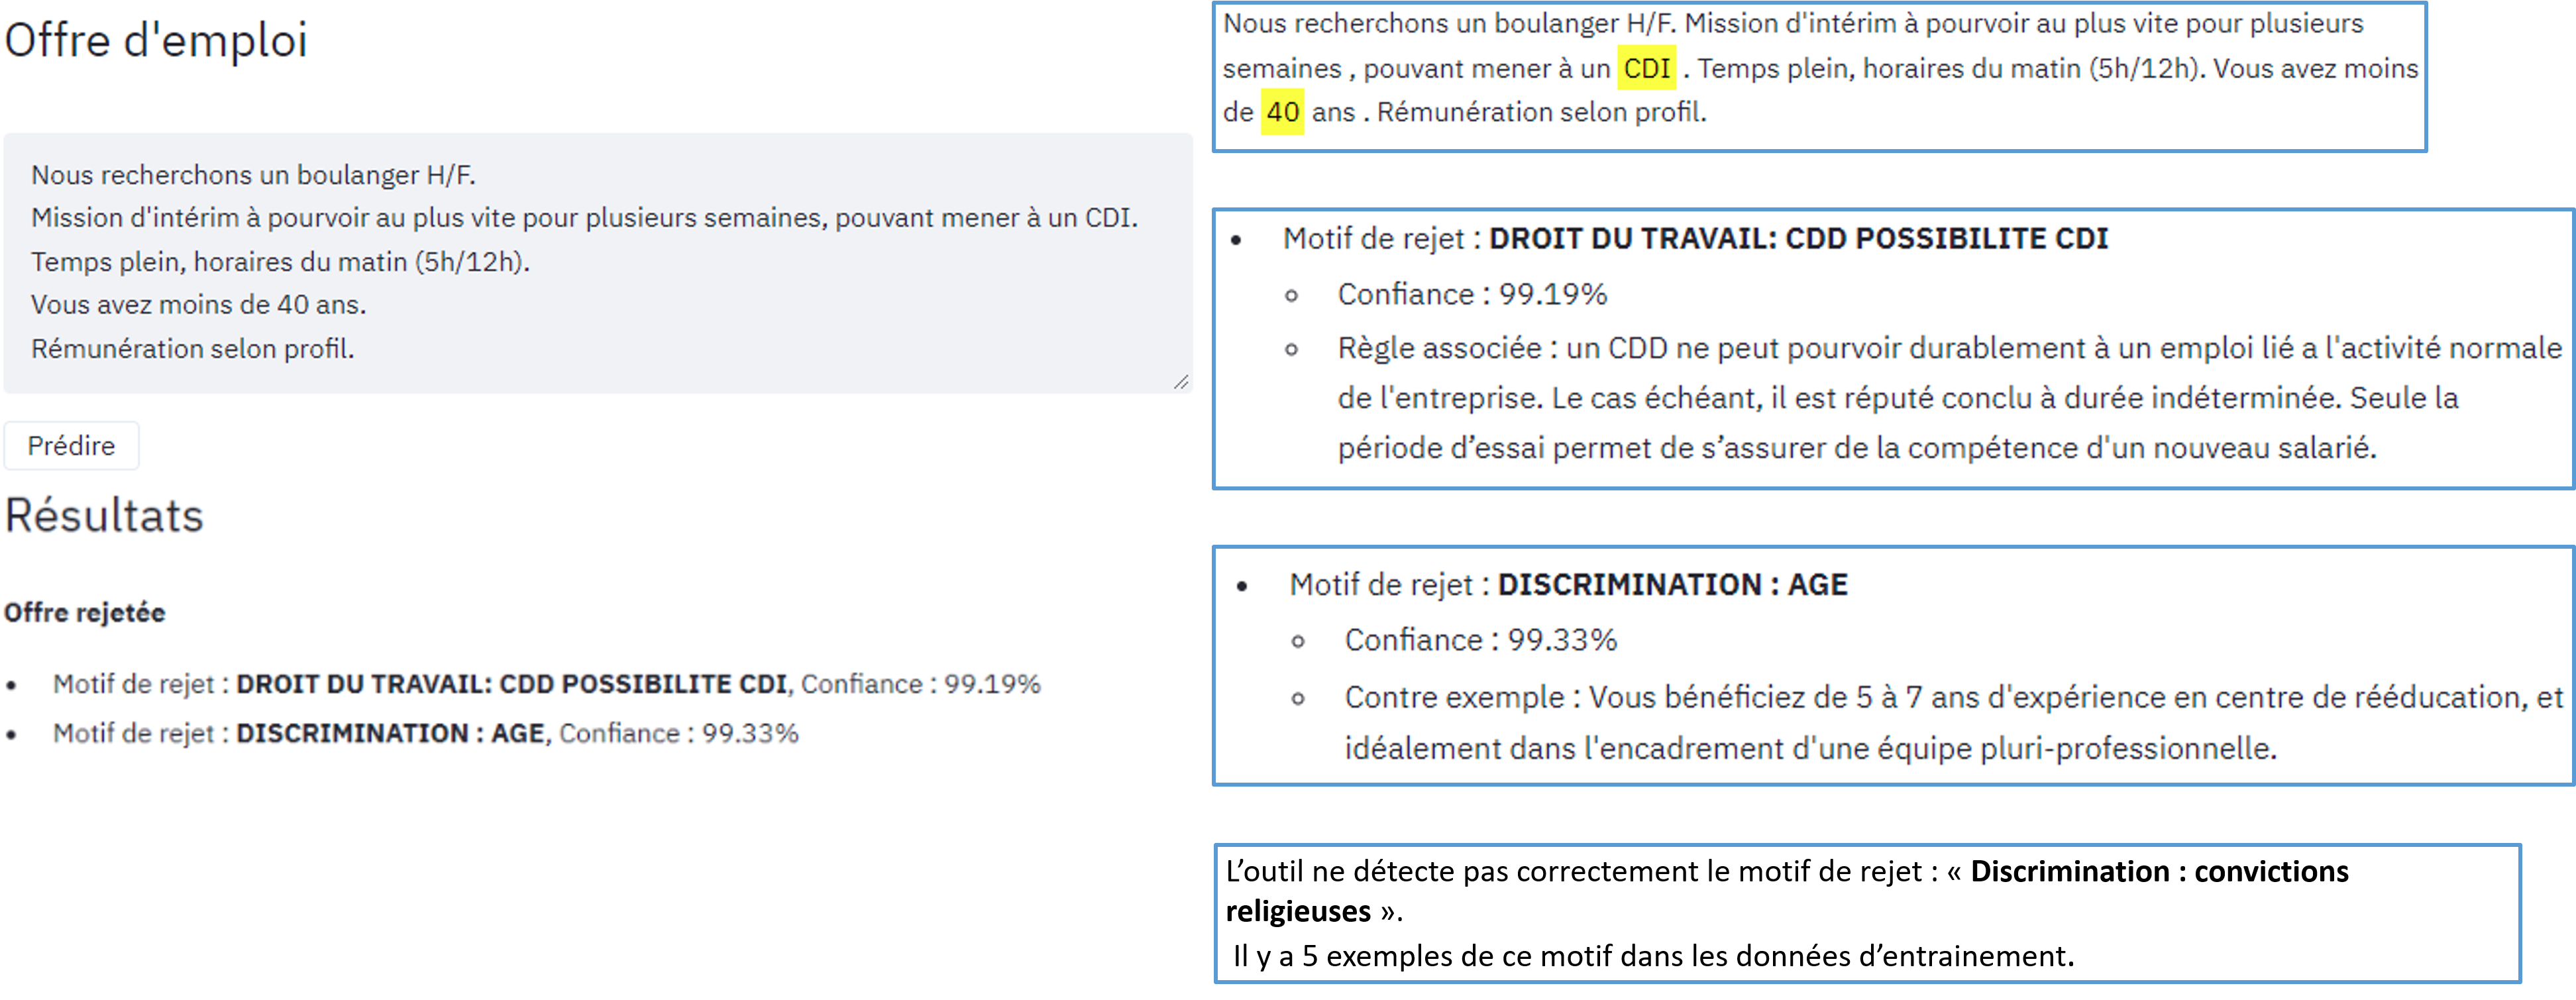
\includegraphics[scale=0.22]{Introduction/figures/format_explications.png}
    \caption{A gauche, exemple d'offre d'emploi rejetée et motifs associés. A droite, les différents formats d'explications possibles. De haut en bas : les variables, règles, exemples, et explications générées.}
    \label{fig:format_exps}
\end{figure}

% feature Based
Les explications basées sur les variables d'entrée mettent en avant une corrélation ou un lien de causalité entre une entrée et une sortie. Ces variables d'entrées peuvent être une colonne de données tabulaires, un n-gramme dans un texte, ou un pixel ou superpixel dans une image.
Ce type d'explication est très utilisé pour l'explicabilité locale, car il s'appuie directement sur une instance donnée en entrée.
Ces explications se font également par contraste : en se concentrant sur les variations menant à des décisions algorithmiques différentes.

% rule Based
Une explication peut se faire en explicitant une règle logique. Cette règle peut mettre en avant une relation de cause à effet du phénomène modélisé, ou sur une corrélation entre une variable et une sortie associée. Dans ce dernier cas, la règle est plus généralisable que l'explication basée sur les variables.
Les explications sous forme de règles peuvent notamment être extraites d'un arbre de décision, ou de contraintes appliquées au système de décision, auquel cas ce sont des explications globales. Elles peuvent aussi être des explications valides dans un périmètre local précis.

% examples Based
Les explications basées sur les exemples sont basées sur des instances réelles du phénomène modélisé. Elles évitent ainsi de s'appuyer sur des données hors distribution, adversaires ou jamais vues par le modèle lors de l'apprentissage. Lorsque c'est un contre-exemple qui est présenté, c'est à dire une instance menant à un résultat différent, alors l'explication est contrastive. Il est également possible de montrer une instance la plus différente possible mais menant au même résultat qu'une instance d'origine, on parle alors d'exemple semi-factuel.

% generated explanations
Enfin, les explications générées ne sont ni des variables, ni des règles, ni des exemples. Elles peuvent correspondre à de la documentation sur le modèle, telle que l'analyse des erreurs du modèle, ou des indications sur ses limites. Elles peuvent prendre la forme de motifs générant de fortes activations de couches d'un réseau de neurones, ou encore des textes et images générés, sans que ces derniers ne ressemblent à un exemple.
% viz montre le fonctionnement des layers~\cite{Zeiler2014}
% Artefact par classe~\cite{Simonyan2014an}
% textes et images générés~\cite{Costa2018}
% model cards :~\cite{Mitchell2019}

\subsection{Données d'applications spécifiques}
Les explications peuvent s'appliquer aux textes, images et données tabulaires. Les textes et images sont des données spécifiques, car analysés directement par les interlocuteurs humains.

Ainsi, le langage naturel est lu, entendu et parlé, et ce dès l'enfance, pour la plupart des humains. Un mot manquant ou une règle de grammaire non respectée sera alors jugée sévèrement. D'un point de vue technique, les textes sont divisibles en n-grammes. Un n-gramme est un ensemble de n entités syntaxiques consécutives, des mots ou des caractères. La figure \ref{fig:n-gramms} illustre ce concept sur un court exemple. Au-dessus de la phrase sont extraits deux bigrammes (ou 2-grammes) de lettres : ``un'' et ``hr'', parmi les 16 possibilités. En dessous sont extraits les bigrammes de mots.

\begin{figure}[htpb!]
    \centering
    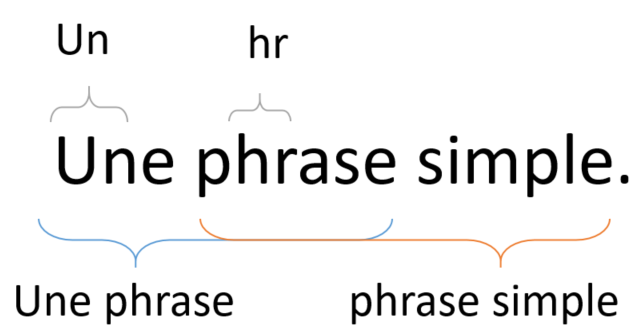
\includegraphics[scale=0.50]{Introduction/figures/n-gramm.png}
    \caption{Exemples de bigrammes de caractères en haut et de mots en bas.}
    \label{fig:n-gramms}
\end{figure}

Pour être traités par un algorithme, les textes doivent être transformés en vecteurs. Les n-grammes peuvent être utilisés directement pour vectoriser le texte, avec des méthodes d'encodage à chaud (``one-hot encoding''). Des techniques plus avancées de sac de mots telles que le TF-IDF (``Term Frequency - Inverse Document Frequency'') peuvent également être employées. Enfin, plus complexe encore, les textes peuvent être vectorisés via un plongement de mots, réseau de neurone spécialisé dans cette tâche.

Les images sont représentables par un ensemble de pixels de couleurs, sur les trois canaux rouge, vert, bleu. Techniquement une image est donc une matrice en trois dimensions : hauteur, largeur, couleur. Il est possible de représenter une image en considérant chaque pixel comme une unité. Les pixels peuvent également être rassemblés par blocs, selon leur similarité. Ces blocs sont des \textit{superpixels}. Ils permettent de découper l'image en blocs porteurs de sens. La figure \ref{fig:illustrations} montre deux images avec des explications au niveau des pixels et superpixels.

\begin{figure}[htpb!]
    \centering
    \begin{subfigure}[b]{0.44\textwidth}
       \centering 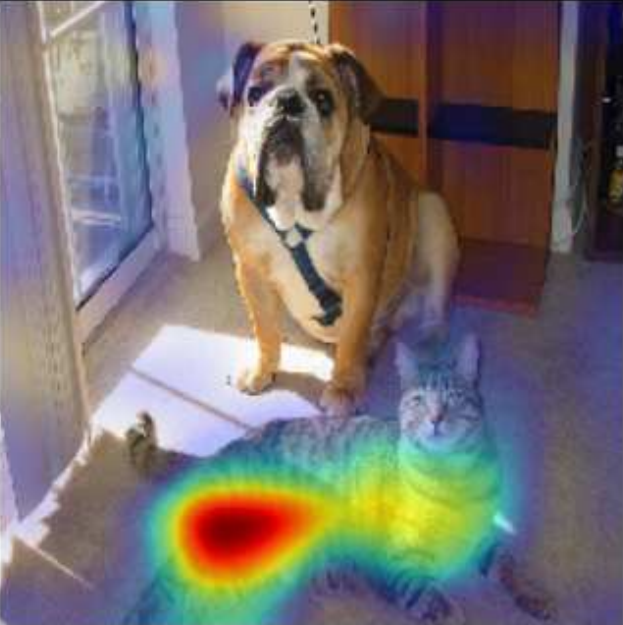
\includegraphics[width=\textwidth]{Introduction/figures/grad-cam.png}
       \caption{Explication au niveau des pixels avec la méthode Grad-CAM~\cite{Selvaraju2017}}\label{fig:gradcam}
    \end{subfigure}
    ~
    \begin{subfigure}[b]{0.44\textwidth}
       \centering 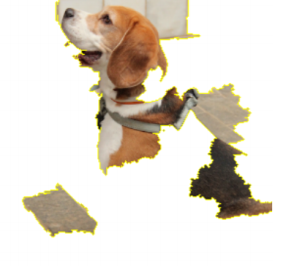
\includegraphics[width=\textwidth]{Introduction/figures/beagle_anchor.png}
       \caption{Explication au niveau des pixels avec la méthode des ancres~\cite{Ribeiro2018}}\label{fig:anchor}
    \end{subfigure}
    \caption{Différentes visualisations d'une explication sur une image.
    }\label{fig:illustrations}
\end{figure}

Enfin, les données tabulaires ont l'avantage de nécessiter moins de transformation entre leur format lisible par un humain et leur intégration dans les modèles. Toutefois, ces données sont moins naturelles à lire comparées aux textes et images.

Les données ne sont pas au choix, à moins de modifier la structure du problème initial. Toutefois elles imposent des contraintes de visualisation et possèdent leurs spécificités propres. Les portées, stratégies, formats, et les données à disposition pour générer des explications sont désormais définies.

Ces différentes caractéristiques des explications impliquent un nombre important de méthodes de génération d'explications. Ces méthodes sont adaptées à certaines caractéristiques.

\section{Comment générer une explication ?}\label{C1:generation}

Les méthodes connues sont présentées en se basant sur le découpage par stratégie, à savoir :
\begin{itemize}
    \item expliquer un modèle boîte noire via des méthodes indépendantes du modèle,
    \item observer un modèle boîte grise avec des méthodes dépendantes du modèle,
    \item concevoir un modèle transparent.
\end{itemize}

\subsection{Explications indépendantes du modèle}

Ce type de méthode a pour principal avantage de pouvoir être utilisé sur tous les modèles. Cela évite de se contraindre techniquement dans le choix d'un modèle. Les explications sont le plus souvent basées sur les variables d'entrées.
Les explications sont générées en considérant le modèle comme une boite noire. Elles relèvent donc de la corrélation plus que de la causalité.

\paragraph{Distillation de connaissance}
Une manière de rendre les modèles interprétables est de se concentrer sur des architectures simples. La distillation de connaissances dans les modèles permet d'entraîner un ensemble complexe de réseaux de neurones et transférer les structures apprises à un réseau de neurones plus simple~\cite{Hinton2015}. Instinctivement, il est tentant de se dire qu'un réseau plus simple pourrait être plus interprétable. Les auteurs de~\cite{Dhurandhar2017} proposent de mesurer l'interprétabilité comme étant le ratio entre la performance du modèle simple et du modèle complexe. En appliquant ces mesures sur un cas d'étude avec un réseau de neurones complexe et un réseau de neurones simplifié, ils en déduisent que la distillation améliore la robustesse, c'est à dire à la résistance aux attaques par modifications subtiles des entrées du modèle, au détriment de l'interprétabilité. En revanche, la distillation est également utilisée pour créer des arbres de décision~\cite{Liu2018,Wu2017} ou des arbres boostés par le gradient~\cite{Che2015} à partir de réseaux de neurones, ce qui revient à créer un module d'explication sous forme d'arbres de décisions. Si l'approche est décrite pour des réseaux de neurones, elle est applicable à d'autres modèles.

\paragraph{Importance des variables}
De nombreuses méthodes fonctionnent sur la quantification de l'importance des variables.
Les vecteurs d'explication locale quantifient l'importance de chaque variable d'entrée pour une instance donnée~\cite{Baehrens2010}. Un vecteur d'explication indique dans quelle direction changer une variable pour que le modèle change de résultat.
En observant un ensemble de vecteurs, on peut également avoir une visualisation plus globale du modèle.
Toutefois, ces vecteurs sont difficilement interprétables pour les utilisateurs, surtout dans le cas de l'analyse sémantique où la dimension est la taille du vocabulaire du corpus.

Les valeurs de Shapley donnent un aperçu de la contribution d'un élément dans un ensemble par rapport à un résultat final~\cite{Strumbelj2010}. La dimension des explications obtenues est égale à la dimension des données en entrée. Elles nécessitent donc un traitement a posteriori pour en retirer des explications claires.
Le calcul des valeurs de Shapley nécessite d'avoir accès au jeu de données d'entraînement du modèle, ce qui est une limitation forte et sous-entend un calcul éventuellement long. Pour limiter le temps de calcul, une estimation des valeurs de Shapley est donnée dans le module SHAP (``SHapley Additive exPlanation'')~\cite{Lundberg2017}.

La méthode Randomized Input Sampling for Explanation (``RISE'') masque aléatoirement des variables en entrée du modèle, pour déterminer les variables importantes~\cite{Petsiuk2018}.
Ces travaux sont approfondis pour créer des cartes de saillance (saliency maps) adaptées à chaque classe du modèle~\cite{Thakur2021}.
Les mesures d'influence quantitative des entrées donnent également le lien entre les données en entrée et les sorties d'un algorithme~\cite{Datta2016}. Cette méthode est intéressante pour sa rapidité de calcul.
La méthode COnstrained feature perturbation and COunterfactual instances (``COCO''), calcule ces poids de variables en contraignant les perturbations dans une direction choisie~\cite{Fang2021}. Malgré ces contraintes, cette méthode nécessite un long temps de calcul. Les contraintes sur les perturbations, basées sur les connaissances fonctionnelles des données, permettent également de créer des explications plus concises~\cite{Gorji2022}.


\paragraph{Approximation linéaire locale}
La méthode Local Interpretable Model-agnostic Explanations (``LIME'') mesure l'importance des variable en effectuant des perturbations aléatoires~\cite{Ribeiro2016}. LIME fonctionne par approximation linéaire du modèle autour d'une instance donnée. C'est ce modèle linéaire qui est ensuite utilisé pour générer des explications. Ces explications correspondent aux variables d'entrée qui impactent le plus la sortie du modèle. Pour l'analyse de texte, ce sont les mots du texte associés à une quantification de l'influence, positive ou négative, sur la réponse du modèle.

Dans le même article, les auteurs présentent SP-LIME, une méthode d'explication globale se basant sur les explications locales de LIME. Un ensemble d'exemples et explications locales associées est ``sélectionné judicieusement''\cite{Ribeiro2016}, étant donné un nombre $B$ prédéfini d'instances à présenter à un utilisateur.
Cette sélection s'appuie sur la recherche d'un ensemble optimal d'exemples couvrant les variables d'entrées les plus importantes. L'ensemble des exemples doit être expliqué par Lime avant d'être sélectionné par SP-Lime.
Cette méthode est intéressante car elle est généralisable au-delà de LIME~\cite{Ribeiro2018}. Par contre, elle nécessite de générer en amont toutes les explications des instances d'un ensemble de données pour pouvoir les sélectionner ensuite.

L'avantage de cette approximation linéaire est la simplicité de la création de l'explication. Toutefois il faut faire l'hypothèse forte que le modèle se comporte linéairement autour de l'instance expliquée. De même, les explications manquent de stabilité, et deux entrées très proches peuvent avoir des explications très différentes. Il est ainsi difficile pour un utilisateur humain de savoir à quel point ces explications sont généralisables.
Les perturbations de LIME sont adaptables à des domaines spécifiques, comme cela est montré dans le cadre de l'analyse d'images~\cite{Stieler2021}.


\paragraph{Ancres}\label{paragraph:anchors}
Les auteurs de LIME ont proposé une amélioration de leur méthode, les Ancres~\cite{Ribeiro2018}. En conservant l'idée d'approximation locale du modèle, les auteurs sont passés d'une approximation par un modèle linéaire à une explication sous forme de règle. L'idée est de mieux définir le contexte dans lequel l'explication générée est valable.
% Une ancre est définie comme un ensemble de variables partagé par des entrées menant à un même résultat en sortie du modèle expliqué.
Soient un modèle $f : X \rightarrow Y$, une instance $x \in X$, un résultat $y \in Y$ choisi, et une ancre $A$ associée. $A$ est une condition telle que si $x$ respecte cette condition, alors la probabilité que $f(x) = y$ est grande. L'ancre est construite de sorte à maximiser cette probabilité, il est toutefois possible que $f(x) \neq y$.
On note $D(.|A)$ l'ensemble des $x \in X$ qui respectent la condition $A$. Une ancre intéressante s'applique à un ensemble $D(.|A)$ le plus grand possible relativement à $X$.
Si les entrées sont des textes, une ancre est un ensemble de mots ou n-grammes.

Dans l'exemple illustré en Fig.~\ref{fig:anchors_domain}, le modèle étudié classe des phrases selon deux catégories : ``positive'' et ``négative''. L'instance d'origine est la phrase ``This movie is not bad'', et est classée ``positive''. L'ancre associée est la règle $A = \{not, bad\} \rightarrow Positive $.
L'ensemble $D(.|A)$  de la Fig.~\ref{fig:anchors_domain_1}, représenté par un rectangle dans la Fig.~\ref{fig:anchors_domain_2}, regroupe les entrées possédant les variables de l'ancre. Dans notre exemple, $D(.|A)$ correspond aux textes comprenant les mots ``not'' et ``bad'' de l'ensemble des variations de l'instance d'origine (ensemble $D$ de la Fig.~\ref{fig:anchors_domain}). L'ensemble $D$ est obtenu en appliquant des variations cohérentes à l'instance d'origine. Appliqué à l'exemple, cela correspond à remplacer un ou plusieurs mots de la phrase par des mots de nature similaire. Remplacer un adjectif par un autre adjectif est une variation cohérente de l'instance d'origine.

\begin{figure}[htpb!]
    \centering
    \begin{subfigure}[b]{0.22\textwidth}
       \centering 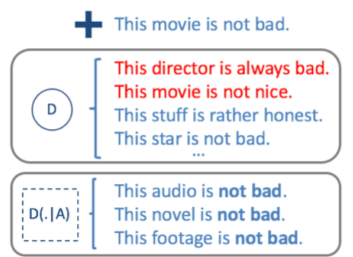
\includegraphics[width=\textwidth]{S1-Comment_evaluer_une_explication/figures/anchors_domain_1.png}
       \caption{Une entrée, ses variations $D$ et leur sous ensemble correspondant à l'ancre $D(.|A)$  }\label{fig:anchors_domain_1}
    \end{subfigure}
    ~
    \begin{subfigure}[b]{0.20\textwidth}
       \centering 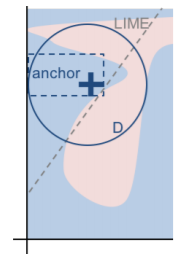
\includegraphics[width=\textwidth]{S1-Comment_evaluer_une_explication/figures/anchors_domain_2.png}
       \caption{Représentation de l'entrée (croix), et des ensembles $D$ (cercle) et $D(.|A)$ (rectangle)}\label{fig:anchors_domain_2}
    \end{subfigure}
    \caption{Textes similaires à une entrée $D$ et son sous ensemble $D(.|A)$ correspondant à l'ancre $\{not, bad\} \rightarrow Positive $. Source:~\cite{Ribeiro2018}}
    \label{fig:anchors_domain}
\end{figure}

Pour sélectionner une ancre, les auteurs choisissent de maximiser deux paramètres. Le premier est la précision, qui est maximale si les éléments de l'ensemble $D(.|A)$ ont la même sortie que l'instance d'origine. Le second est la couverture, soit la taille de l'ensemble $D(.|A)$ par rapport à l'ensemble $D$. Une ancre avec une forte précision est une explication fidèle au modèle boîte noire. Si elle a une bonne couverture, une ancre est assez généralisable.

Le travail autour des ancres met en avant la relation entre l'utilisateur et l'explication. La limite de LIME contournée par les Ancres est la difficulté pour l'utilisateur à déterminer la validité d'une l'explication donnée. Ce faisant, l'explication donnée, à savoir une règle, est également plus facile à aborder qu'un ensemble de poids comme le résultat de base de LIME.\\

Les explications indépendantes des modèles sont une première approche en considérant les modèles boîtes noires, mais il s'agit plus de mettre en avant des corrélations entre les entrées et les résultats du système.
Pour aller plus loin, il est possible de s'appuyer sur la structure du modèle pour générer des explications. La \textit{boîte noire} devient alors une \textit{boîte grise}.

\paragraph{Génération de contre-exemples}
% basé sur les perturbations
Les méthodes basées sur la perturbation telles que LIME~\cite{Ribeiro2016} et RISE~\cite{Petsiuk2018} créent des données hors distribution (\textit{out of distribution}, OOD). Ces échantillons OOD peuvent être mal classés par les modèles, mais peuvent aussi être assez inhabituels pour les utilisateurs finaux, perdant ainsi la clarté des explications. Ceci est particulièrement vrai dans le domaine du langage naturel, où le texte OOD devient très rapidement dénué de sens. Cette déviance par rapport à la distribution originale des données peut être mesurée~\cite{Qiu2021}.
% contraintes sur les perturbations
Des travaux tentent de contraindre les perturbations, en veillant à ce que les données générées soient cohérentes avec la distribution des données d'apprentissage. Cela peut être réalisé en trouvant le meilleur masque de perturbation~\cite{Chang2019} et en remplissant ce masque de la meilleure façon possible pour créer une entrée cohérente~\cite{Agarwal2020}.


% GANs
Pour aller plus loin, des entrées cohérentes peuvent être générées directement via des Réseaux antagonistes génératifs (Generative Adversarial Networks, GAN), en produisant des exemples factuels, des exemples semi-factuels et des exemples contrefactuels~\cite{Kenny2021,Charachon2021}. Ces points de données générés sont similaires à des données d'entraînement par conception, évitant la plupart des problèmes d'OOD, selon les performances du GAN. De plus, ces exemples aident les utilisateurs finaux à reconstruire un modèle mental, c'est à dire une représentation mentale du modèle. En effet, ils rendent tangibles les limites de décision, situées entre les exemples semi-factuels et contrefactuels. La mise en évidence du delta nécessaire pour franchir cette frontière peut être obtenue en calculant la différence entre les instances factuelles et contrefactuelles~\cite{Charachon2021}.

% Sobriété
Cependant, le gain en explicabilité apporté par certaines méthodes de pointe se fait au détriment du temps de calcul, et de la sobriété énergétique. A titre d'illustration, citée par~\cite{Chang2019}, une approche d'explication avec un masque de perturbation cohérent peut prendre ``environ une minute sur un seul GPU pour terminer une image''.

% SVM ?


\subsection{Explications dépendantes du modèle}

Les explications dépendantes du modèle sont basées sur l'observation des paramètres du modèle après son entraînement. Cette observation, pour conserver la métaphore de la boite noire, revient à ouvrir cette boite et regarder à l'intérieur. Les explications sont alors plus fidèles au fonctionnement du système étudié que les méthodes indépendantes du modèle. Toutefois, cette approche contraint fortement le choix du modèle.

\paragraph{Réseaux à convolutions}
Dès 2013, des travaux sur les réseaux de neurones proposent des visualisations de leur fonctionnement, dans le cadre de la classification d'images. Dans~\cite{Zeiler2014}, les auteurs proposent de mieux appréhender le fonctionnement des réseaux à convolution (Convolutionnal Neural Networks, CNN), par une visualisation directe des motifs d'activation des neurones par couche. Ils utilisent pour cela un réseau de neurones appelé \textit{Deconvolutionnal Network}. Ils obtiennent des motifs reconnus par chaque couche, motifs simples sur les couches basses et plus semblables aux classes détectées sur les couches hautes. Les auteurs vérifient également le comportement de leur modèle en masquant certaines parties des images et en observant les éventuelles variations de classification induites.

Toujours sur les CNN, la méthode de cartographie d'activation de classe, (Class Activation Mapping, CAM)~\cite{Zhou2016} est proposée. Elle permet de générer des cartes de chaleur des endroits de l'image aidant à la détection d'une classe en particulier.   .
La méthode Grad-CAM~\cite{Selvaraju2017} mélange les visualisations à celles de~\cite{Springenberg2015,Zeiler2014}, afin d'obtenir les parties de l'image ainsi que les motifs précis permettant la classification (Fig~\ref{fig:gradcam}).
Ces travaux sont repris par ~\cite{Chattopadhay2018} pour donner l'amélioration \textit{Grad-CAM++}.
Dans la continuité de cas travaux, des concepteurs ont été associés à ces trois méthodes~\cite{Qian2022}. Un concepteur est un motif de changements d'états de neurones. Les auteurs proposent grâce aux concepteurs de prendre en compte les éléments en faveur et en défaveur de la classification. Toutefois, les cartes de chaleur issues de cette méthode sont plus diffuses.
Des travaux sont également effectués sur les cartes de saillances (saliency maps) des images~\cite{Simonyan2014}. Ces travaux permettent d'avoir une indication fidèle du fonctionnement du modèle. Ces techniques sont plutôt orientées analyse d'image.

\paragraph{Long-Short Term Memory (LSTM)}
Dans la même philosophie, les auteurs de~\cite{Karpathy2016} essaient de comprendre les forces et les limites des réseaux de neurones de type LSTM, appliqués à l'analyse de textes.
Pour leur analyse, ils génèrent des visualisations sur des motifs spécifiques dans les données entraînant les activations de certaines cellules. Un exemple donné par les auteurs et présenté en figure~\ref{fig:lstm_quotes} concerne l'activation de certaines cellules en fonction des caractères rencontrés dans un texte. La visualisation met en évidence la détection du texte entre guillemets.

\begin{figure}[htpb!]
\centering
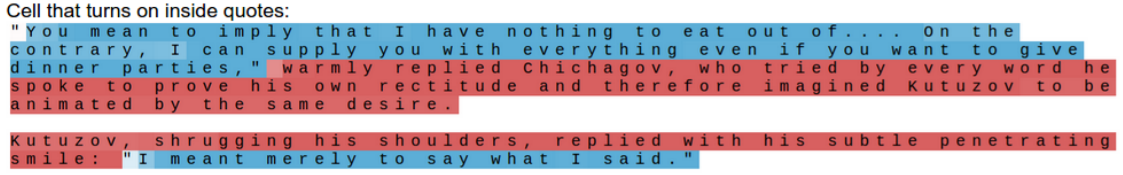
\includegraphics[width=\textwidth]{S1-Comment_evaluer_une_explication/figures/lstm_quotes_activation.png}
\caption{Activation d'une cellule en fonction des guillemets dans le texte. Source :~\cite{Karpathy2016}}
\label{fig:lstm_quotes}
\end{figure}

Ce type de réseau de neurones est largement utilisé dans l'analyse sémantique.
Les visualisations peuvent donner une idée précise du fonctionnement du modèle. Toutefois, elles sont complexes ou nécessitent un travail de recherche et d’analyse, d’autant plus si on considère chaque cellule.
Pour donner un ordre d'idée, des structures de LSTM de la littérature peuvent avoir 300~\cite{Lin2017} ou encore 512~\cite{Karpathy2016} cellules. Il convient alors de toutes les explorer pour trouver, pour une petite partie d'entre elles, des activations significatives.
Si ce type d’approche permet de mieux comprendre les indices utilisés par le réseau, il ne s’agit pas forcément d’une explication de la décision finale. L'inspection neuronale profonde (Deep Neural Inspection, DNI) repose sur les activations de la couche d'états cachés d'un LSTM de taille restreinte, afin de vérifier le respect de fonctions hypothèses définies par des experts des données, telles que la recherche d'éléments spécifiques dans les données : ponctuation pour du texte, couleurs pour les images, etc.~\cite{Sellam2019}.



\paragraph{Décomposition du modèle}
La décomposition pixel par pixel (\textit{Pixel-Wise Decomposition}, PWD) est une stratégie permettant d'expliquer les résultats d'un classifieur d'images en créant une carte de chaleur des pixels les plus pertinents pour une prédiction donnée~\cite{Bach2015}.
Pour calculer la pertinence $R$ (\textit{Relevance}) de leurs variables d'entrée, dans leur exemple des pixels. Ils décomposent la prédiction $f(x)$ comme étant la somme des contributions des neurones de la couche précédente et appliquent itérativement cette propriété jusqu'à arriver à la couche d'entrée de leur réseau. Les auteurs décrivent deux manières d'y parvenir.
La première méthode est la propagation de pertinence couche par couche (\textit{Layer-wise Relevance Propagation}, LRP), un concept regroupant diverses solutions de décomposition respectant certains critères. La seconde est une approche basée sur la décomposition de Taylor, qui permet une approximation de la propagation de pertinence couche par couche, en s'appuyant sur le principe de décomposition de fonctions pour décomposer directement le classifieur $f$.
Ces travaux sont approfondis dans~\cite{Montavon2017} où les auteurs proposent la \textit{Deep Taylor Decomposition}, qui est une adaptation de la décomposition de Taylor, appliquée non pas au modèle entier mais à chaque fonction de pertinence $R_j({x_i})$ entre un neurone $j$ d'une couche $n$ et les neurones ${x_i}$ de la couche $n-1$.
Dans ce dernier article les auteurs illustrent leurs travaux avec des réseaux de neurones classant des images, mais ce type de méthode peut être appliqué à d'autres modèles et peut également être élargi à d'autres types d'entrées, comme les textes dans~\cite{Montavon2017}.
L'analyse des éléments du modèle peut être encore plus visuelle comme avec les graphes de flux de données intégrés à la librairie de développement de modèles Tensorflow~\cite{Wongsuphasawat2017}.
L'apprentissage profond de variables importantes (Deep Learning Important FeaTures, DeepLIFT)~\cite{Shrikumar2017} utilise la rétropropagation des contributions des neurones, similairement à la LRP~\cite{Bach2015}. Les auteurs définissent ces contributions comme positives ou négatives, relativement à une contribution de référence~\cite{Shrikumar2017}.
Il est également possible de déterminer des vecteurs concepts, permettant de proposer des exemples correspondant à des concepts sémantiques pertinents sur le plan fonctionnel~\cite{Kim2018}.

Les méthodes décrites précédemment permettent de mieux appréhender le fonctionnement des modèles, en se basant sur leurs caractéristiques respectives. Toutefois ces méthodes, dépendantes ou indépendantes du modèle, nécessitent des calculs ou de l'analyse d'un grand nombre d'éléments.
 Pour éviter cela, la dernière approche est de créer un modèle dont la structure même le rend plus transparent.

\subsection{Modèle Interprétable}
L'idée de modèle transparent est de limiter le besoin en analyse post entraînement en s'appuyant sur des structures spécifiques du modèle. De cette manière une meilleure fidélité au modèle est assurée tout en limitant les calculs et approximations.


\paragraph{Architectures simplifiées}
Dans le courant de simplification des réseaux, des expérimentations mettent en évidence l'efficacité d'architectures de réseaux de neurones simplistes mais capables de résoudre des problèmes complexes, comme le stationnement d'une voiture miniature~\cite{Hasani2018}. Ce type de réseau possède une topologie inspirée du système nerveux du ver \textit{C. elegans}. Le papier définit un réseau ainsi constitué de 12 neurones, en l'entraînant sur la tâche de stationner un robot.
En observant les activations des neurones en fonction des phases, les auteurs mettent en lumière le rôle des neurones dans chaque phase de la tâche accomplie, en mettant en évidence par exemple les neurones s'activant lorsque le robot doit tourner à droite. Ces activations sont interprétables notamment parce que le réseau est composé de peu de neurones; cela facilitant grandement l'analyse des activations. Cette approche permet ainsi de réaliser un travail similaire à~\cite{Karpathy2016}, qui analyse les activations de cellules LSTM, mais sur un nombre réduit de neurones.

Considérant la représentation de modèles sous forme de fonctions, l'approche Model Learning with Personalized Interpretability Estimation (ML-PIE) permet à l'utilisateur de choisir successivement les fonctions qui lui semblent les plus explicables,  permettant la génération d'un modèle spécifiquement adapté à leur besoin~\cite{Virgolin2021}.

\paragraph{Mécanismes d'attention}\label{paragraph:attention}
Les mécanismes d'attention dans les réseaux de neurones sont une manière de rendre les modèles directement plus interprétables\cite{Bahdanau2015}. L'attention est appliquée dans diverses architectures de réseaux, dont les transformeurs qui reposent essentiellement sur ce mécanisme~\cite{Vaswani2017, Abnar2020}. Dans~\cite{Lin2017}, les auteurs créent un plongement de mots via un réseau avec une partie LSTM et une partie basée sur l'attention. Chaque phrase est représentée par une matrice $M = AH$, où $A$ est la matrice d'attention et $H$ les états cachés de la couche LSTM. Les vecteurs d'attention $a$ composant $A$ vont se concentrer sur des aspects différents de la phrase. En sommant et normalisant (par une fonction softmax) tous les vecteurs d'attention $a$, les mots fortement considérés par le plongement ressortent avec les poids les plus forts.
Cette solution permet donc d'avoir une visualisation claire des variables importantes en entrée du réseau, en observant les paramètres du modèle. Un exemple de visualisation est présenté dans le cadre de la traduction de textes dans~\cite{Olah2016} (Fig.~\ref{fig:lstm_attention}). Elle met en avant l'inversion des mots entre l'entrée en anglais (``\textit{european economic area}'') et la traduction française (``\textit{zone économique européenne}''). La visualisation des poids d'attention est également utilisée dans~\cite{Wang2016} afin de valider l'intérêt de leur topologie de réseau, également composé d'un LSTM et d'une couche d'attention. Le principal intérêt de l'analyse de l'attention est qu'il n'y a pas besoin de calculs supplémentaires d'une métrique spécifique une fois le modèle entraîné, contrairement à~\cite{Bach2015} par exemple.

\begin{figure}[htpb!]
\centering
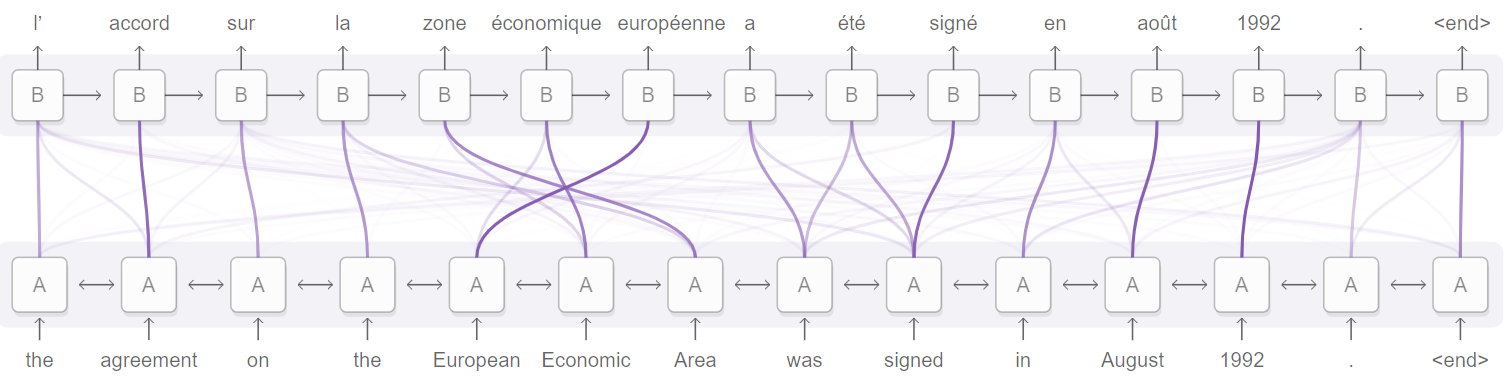
\includegraphics[width=\textwidth]{S1-Comment_evaluer_une_explication/figures/lstm_attention.png}
\caption{Visualisation de l'attention pour une tâche de traduction. Source:~\cite{Olah2016}}
\label{fig:lstm_attention}
\end{figure}

Un modèle peut également utiliser l'attention pour enrichir les données d'apprentissage. Une méthode possible est d'associer les éléments d'attention à des prototypes de données connus qui permettent la prise de décision~\cite{Barnett2021}. Le modèle est ainsi basé sur le raisonnement humain. Une autre façon de faire consiste à superposer des données et des cartes d'attentions issues de l'attention visuelle d'humains effectuant la même tâche que le modèle à entraîner~\cite{Obeso2022}.
Des mécanismes similaires ont été développés sur les modèles linéaires généralisés (Generalized Linear Models, GLM) afin d'en extraire des poids d'attention~\cite{Richman2021}.

\paragraph{Génération d'explications}
Certains systèmes peuvent également générer d'eux même des explications autour d'une décision. C'est le cas de~\cite{Costa2018} où les explications d'un système de recommandation sont générées sous forme de critiques d'utilisateurs (``\textit{I wouldn’t recommend it.}'') via un LSTM. Le principe de l'expérimentation est de reconstruire une critique que produirait un utilisateur avec un texte le plus naturel possible. Les auteurs évaluent leurs explications avec des métriques de lisibilité de textes tel que le score \textit{Flesch-Reading-Ease}. Si le système de recommandation n'est pas nécessairement un réseau de neurones, un système similaire peut être appliqué à tout système de prédiction basé sur des textes.
Ces explications générées peuvent être plus globales, comme les cartes de modèles, reprenant un ensemble structuré d'informations concernant un modèle~\cite{Fang2020}.

D'autres architectures de modèles apprennent des concepts non supervisés dans les données. Les réseaux de neurones auto-explicatifs (Self-Explaining Neural Network, SENN) utilisent l'architecture encodeur-décodeur pour apprendre ces concepts~\cite{AlvarezMelis2018}. Certains montrent l'activation neuronale associée à des éléments de concept, tels que les couleurs dans le cadre de l'analyse d'images~\cite{Barberan2022}.
Ces concepts peuvent être supervisés, c'est le cas des modèles de goulots d'étranglement conceptuels (Concept Bottleneck Models, CBM), qui apprennent à associer une entrée à un ensemble de concepts, présents dans les données d'entraînement, puis les ensembles de concepts à une classe~\cite{Koh2020}.
Une fusion des concepts supervisés et non supervisés de~\cite{AlvarezMelis2018,Koh2020} intègre à la fois l'expertise métier et la découverte de nouveaux concepts~\cite{Sawada2022}.
Similairement aux concepts, des prototypes de granularité modulable peuvent être présentés, issus des motifs présents dans les données d'entraînement du modèle~\cite{Uehara2020}. Le dictionnaire de prototypes associés peut être directement appris par le modèle, ~\cite{Uehara2021,Yun2021}. Dans le cadre de l'analyse des séries temporelles, la méthode eXplainable Representation of Complex System Behavior (XR-CSB) extrait ces concepts correspondant à des états~\cite{Kaadoud2022}. XR-CSB permet de générer des explications sous la forme d'automates à états.


Les principales méthodes d'explicabilité ont été abordées, proposant un aperçu de la multiplicité des propositions de la communauté. Chaque méthode possède ses avantages et inconvénients. La section suivante couvre l'état de l'art de l'évaluation de ces méthodes.


\section{Comment évaluer une explication ?} \label{C1:evaluations}

Évaluer les méthodes d'explicabilité n'est pas systématiquement réalisé dans la littérature. Toutefois de nombreuses méthodes sont présentées dans ce chapitre, associées aux points qu'elles permettent d'évaluer.

Les méthodes d'évaluation sont basées sur des mesures tirées des explications elles même, ou s'appuient sur le ressenti utilisateur ou l'impact d'une explication dans une tâche~\cite{Ayyar2021, Dodge2020}. Le choix d'une méthode adaptée rend compte non seulement de la qualité d'une explication mais aussi de son adéquation avec les objectifs de l'outil global dans la réalisation d'un acte métier.

Cette section présente les différentes méthodes d'évaluation des explications, à l'état de l'art.
% Plan
La section \ref{C1:proprietes} définit les propriétés souhaitables pour une explication, recoupant et regroupant les noms parfois différents dans la littérature. Il vise à aider la sélection d'une ou plusieurs propriétés à maximiser, ce qui guidera le choix d'une méthode d'évaluation par la suite.
La section \ref{C1:utilisateurs} définit les avantages et inconvénients de deux types de protocoles, ceux faisant appel à des utilisateurs et ceux qui s'en détachent. L'intégration d'humains dans un protocole expérimental apportant un travail conséquent, ce choix doit être réfléchi et motivé.
Les sections \ref{C1:ev_obj} et \ref{C1:ev_subj} présentent les méthodes d'évaluation de la littérature, les liant aux propriétés qu'elles permettent d'évaluer.
Enfin, la section \ref{C1:debat} met en avant les challenges du domaine dans le lien entre évaluation technique et évaluation humaine.


\subsection{Propriétés souhaitées} \label{C1:proprietes}

% objectif
Les propriétés souhaitées des explications sont nombreuses. Cette section les regroupe en harmonisant les notations de l'état de l'art quand cela est possible.
% Plan
Dans un premier temps, les propriétés qui conviennent à toutes les explications seront citées avant d'être détaillées.

Les propriétés des explications sont souvent appelées avec des noms variables dans la littérature. Toutefois, il est possible de les regrouper sous des adjectifs suffisamment génériques.

\paragraph{Fidèle}
La fidélité correspond à la capacité d'une explication à être en accord avec le phénomène ou modèle expliqué~\cite{Guidotti2018,Lundberg2017,Lakkaraju2019,Ribeiro2018,Hoffman2018,Liu2021,Ciravegna2020}.
Pour~\cite{Codella2019} cela signifie qu'elle est argumentée ; elle s'appuie sur des éléments vérifiables par le receveur. Pour une tâche de classification d'images de chien, cela signifierai souligner des éléments que le receveur sait être différenciant : forme des oreilles, du museau, etc. Pour~\cite{Petsiuk2018, DeYoung2019} elle comporte donc les éléments minimaux permettant la prise de décision.

\paragraph{Interprétable}
L'interprétabilité d'une explication est une notion plus complexe. Pour~\cite{Guidotti2018,Virgolin2021,Lakkaraju2019} cela correspond à la taille d'un modèle élève générant les explications, donnant ainsi une explication de taille raisonnable.~\cite{Ribeiro2016} abonde dans ce sens en indiquant qu'une explication interprétable possède un nombre limité d'éléments et s'appuie sur des notions adaptées à son receveur. Pour~\cite{Gilpin2018} cela signifie que l'explication est suffisamment simple pour être comprise. Il est ainsi possible de découper l'interprétabilité en trois propriétés plus spécifiques : la concision, la complétude et l'adaptation.

\subparagraph{Concise}
Une explication concise comporte un nombre limité d'éléments. Le receveur n'est pas noyé par la quantité d'informations. Si de nombreux travaux y font référence~\cite{Ribeiro2016,Petsiuk2018, Poppi2021,Lakkaraju2019,Zafar2021a},~\cite{Miller2017} va plus loin, mettant en avant le fait que les receveurs ont une forte tendance à favoriser les explications les plus courtes.
\cite{Gilpin2018} met en garde contre le biais humain qui, en favorisant les explications courtes, risque de préférer des systèmes d'explications persuasifs plutôt qu'interprétables. Ces systèmes s'appuient alors sur des connaissances et préférences des receveurs, quitte à être moins fidèles~\cite{Herman2017}.

\subparagraph{Auto-explicative}
Une explication est auto-explicative lorsqu'elle ne nécessite pas de connaissances supplémentaires pour être comprise~\cite{Codella2019,Gilpin2018}. Par exemple, une équation sera facilement interprétable pour un expert de la donnée, mais pas pour un receveur n'ayant pas l'habitude de manipuler ce format d'information~\cite{Ribeiro2016}. Elle comporte donc tous les éléments nécessaires à sa compréhension sans qu'il soit nécessaire de les détailler~\cite{Hoffman2018}.

\subparagraph{Adaptée aux receveurs}
Une explication adaptée aux receveurs est conçue dans un vocabulaire connu de ces derniers, par exemple en intégrant le vocabulaire spécifique à la tâche ou domaine métier associé~\cite{Codella2019}.
\cite{Dam2018, DeYoung2019} abondent en ce sens, estimant qu'elle pourrait ressembler aux explications que fourniraient des humains qui auraient la même tâche. Dans cette même dynamique mais spécifique au TALN, les travaux de~\cite{Zafar2021a} montrent que les utilisateurs ont une préférence pour les explications de textes basées sur des phrases plutôt que sur des mots.

\paragraph{Représentative}
Une propriété associée est la non-ambigüité, définie par~\cite{Lakkaraju2019} pour un ensemble de règles, comme le respect à la fois d'une bonne couverture des règles, et d'un faible empiètement des règles les unes entre les autres~\cite{Lakkaraju2019}.

\paragraph{Utile}
Enfin, l'utilité des explications met en avant son intérêt pour les receveurs selon leurs attentes~\cite{Miller2017,Hoffman2018}. Si le receveur est un scientifique des données, manager ou régulateur, cela correspond à détecter des biais~\cite{Gilpin2018}.
Pour un expert du domaine ou une personne concernée par l'usage du modèle, l'utilité peut être une meilleure représentation mentale du comportement du modèle, le modèle mental~\cite{Arrieta2020,Ribeiro2018,Dam2018,Mohseni2021a}, notamment en détectant mieux ses erreurs~\cite{DoshiVelez2017}.

Pour un utilisateur cela peut l'amener à améliorer sa performance dans l'acte métier associé, ou aller plus vite~\cite{Ribeiro2018, Dhurandhar2017,Gilpin2018,Janssen2020,Mohseni2021a}. Pour tout utilisateur, l'utilité crée ou améliore sa confiance dans le modèle~\cite{Hoffman2018,Mohseni2021a}. Dans cette même optique,~\cite{Rasouli2022} propose de favoriser la mise en avant de critères actionnables, c'est à dire ceux sur lesquels l'utilisateur peut agir ou conseiller une action.
\vspace{1cm}

Il est difficile de maximiser chaque propriété, notamment parce que certaines sont incompatibles. Ainsi l'auto-explicabilité empêche la concision. Pour chaque projet, un ensemble de propriétés sur lesquelles doit se porter l'effort peut être défini. Ces propriétés étant définies, les sections suivantes définissent les modalités d'évaluation du respect de celles-ci. Dans la section \ref{C1:utilisateurs} est discutée la présence ou non des utilisateurs humains lors de l'évaluation des explications.

\subsection{\'Evaluation avec ou sans utilisateur} \label{C1:utilisateurs}

Les modalités d'évaluation des explications sont dépendantes à la fois des contraintes du projet : temps, argent, disponibilité des différents acteurs, mais aussi des propriétés souhaitées, vues en section précédente. Nous présentons les trois niveaux d'évaluation de la littérature : avec des utilisateurs réels, avec des systèmes simulant le comportement des utilisateurs, ou sans utilisateurs, ni réels ni simulés.

\paragraph{Avec des utilisateurs réels} \label{C1:utilisateurs_reels} % utilisateur ou autre nom ?
% Pourquoi
L'évaluation avec utilisateur permet de valider la bonne adéquation entre l'explication et son receveur. Elle assure notamment que les propriétés d'interprétabilité et d'utilité sont valides.
% Comment
\cite{DoshiVelez2017} divise explicitement les évaluations avec utilisateurs en deux types, observés dans la littérature. Ces évaluations sont :
\begin{enumerate}
    \item l'\'evaluation applicative,
    \item l'\'evaluation humaine
\end{enumerate}

% \item \'Evaluation applicative
Pour l'évaluation applicative, les conditions d'utilisation du modèle doivent être les plus proches possible de la réalité. L'évaluation porte alors sur la compréhension et la préférence de l'utilisateur recevant l'explication. Le profil de cet utilisateur doit correspondre à celui ou ceux auxquels sont destinés les explications. Il est ainsi possible de demander à effectuer l'action métier, avec et sans explications, ou avec des explications différentes, et comparer les performances et la vélocité de l'utilisateur~\cite{Dam2018}. Une évaluation similaire consiste à demander aux utilisateurs de donner une explication au même format, et comparer les deux. Toutefois elle nécessite de travailler sur des modèles simples, elle est donc moins adaptée à l'apprentissage profond~\cite{Lundberg2017, Dam2018}.

% \item \'Evaluation humaine, sur des tâches simples
L'évaluation humaine se fait sur des tâches simplifiées, et non l'acte métier cible. De même elle ne nécessite pas de faire appel spécifiquement au public cible des explications, ce qui est intéressant lorsque ce public est composé d'experts peu disponibles. Une tâche simplifiée peut être :
\begin{itemize}
    \item la comparaison de paires d'explications~\cite{Lakkaraju2019,Dam2018},
    \item la comparaison de modèles simples tels que des petits arbres de décision\cite{Allahyari2011},
    \item l'évaluation qualitative d'une explication pour un cas fonctionnel connu~\cite{Kaadoud2022},
    \item retrouver le même résultat que le modèle, à l'aide de l'entrée et l'explication associée~\cite{Ribeiro2018, Dam2018, Zafar2021a,Lim2009},
    \item sélectionner le ``meilleur modèle'' selon les résultats et explications associées~\cite{Ribeiro2016}.
\end{itemize}
Ces évaluations se font avec un ordre de grandeur de une à plusieurs dizaines d'humains participant : 33 pour~\cite{Lakkaraju2019}, 15 pour~\cite{Zafar2021a}. Quelques expérimentations sont menées à plus grandes échelles comme celle de~\cite{Allahyari2011} dont qui fait appel à 100 personnes, ou celle de~\cite{Lim2009} qui rassemble 158 personnes.

% Avantages
Présenter les explications à un receveur permet de s'assurer de la bonne adéquation entre ce dernier et le format d'explication proposé. Ce type d'évaluation est le plus proche des conditions réelles d'usage des explications, et est donc le plus précis. C'est la seule modalité d'évaluation qui permet de vérifier que le vocabulaire est adapté.
% Inconvénients
Cette précision a un coût non négligeable~\cite{Dam2018, DoshiVelez2017}. Ce type d'évaluation nécessite également de prendre du temps, notamment pour récolter les évaluations des receveurs. Dans le cas où des professionnels sont requis, iels sont parfois très peu disponibles : experts, médecins etc. Ces évaluations sont également sensibles aux biais humains, avec une préférence pour les explications courtes, qui ressemblent à celles que fournirait un humain~\cite{Petsiuk2018,Miller2019,Gilpin2018}.


\paragraph{Avec des utilisateurs simulés}
% Pourquoi
Il est également possible d'évaluer une explication pour son niveau d'informations et son adéquation avec l'acte métier associé. C'est alors la performance au regard de la tâche à accomplir qui est mesurée.
% Comment
Pour mesurer cette performance, quand les utilisateurs sont peu disponibles, il est possible de les remplacer par des algorithmes simulant leur comportement.
% Les utilisateurs réels vus en section précédente sont des humains, avec des expertises pouvant être variées.
Les utilisateurs simulés sont des modèles plus ou moins complexes, tels que des forêts aléatoires ou des réseaux de neurones~\cite{Ribeiro2018}. Ces utilisateurs simulés peuvent effectuer, à l'instar des utilisateurs réels, des tâches complexes ou simplifiées. Il est ainsi possible d'entraîner un classifieur qui va prédire une classe en s'aidant de l'explication pour la retrouver~\cite{Ribeiro2016, Ribeiro2018, Dhurandhar2017}, ou encore choisir le meilleur modèle, grâce aux explications~\cite{Ribeiro2016}.

% Avantages
Ce type d'expérimentation est intéressant dans la mesure où son coût est moindre comparé aux expérimentations avec utilisateurs réels. En particulier, si les utilisateurs ciblés sont des experts, les utilisateurs simulés ont l'avantage de ne pas être limité en nombre ou en quantité de données d'expérimentation traitées. Ils permettent de rester proche de l'acte métier, en simulant cet acte par exemple. Enfin, ils permettent une bonne reproductibilité, facilitant les comparaisons entre méthodes, contrairement aux expériences avec des utilisateurs réels.
% Inconvénients
Toutefois, il n'est pas possible de valider le vocabulaire ou l'acceptation d'un système comme c'est le cas avec des utilisateurs réels.
% On s'appuie sur des modèles pour valider d'autres modèles, potentiellement mal perçu, peut aussi ajouter des biais

\paragraph{Sans utilisateurs} \label{C1:no_user}

% Pourquoi
Enfin, il est possible de valider les propriétés des explications sur de larges jeux de données, sans recourir aux utilisateurs. Dès lors que la propriété est mesurable (définie par une équation), elle peut alors être directement évaluée et comparée.

% Comment
Les évaluations sans utilisateurs se font par la mesure d'une propriété. La concision pourra être associée au nombre de variables remontées dans une explication basée sur ces dernières~\cite{Zafar2021a}. La fidélité pourra correspondre au taux d'erreur d'un système d'explication en regard du phénomène ou modèle qu'il doit expliquer~\cite{Lakkaraju2019}. Dans~\cite{Petsiuk2018}, les éléments constituant l'explication sont supprimés un à un de l'entrée du modèle et l'observation du changement de résultat indique la pertinence de l'explication : plus celle-ci se fait tôt, plus les éléments constituant l'explication étaient nécessaires pour mener au résultat.

% Avantages
Les expérimentations sans utilisateur ont un coût moindre, et une bonne reproductibilité. Ils sont encore plus adaptés à l'évaluation comparative que les utilisateurs simulés, car ils ne nécessitent pas l'entraînement de ces derniers.
% Inconvénients
Toutefois, ils sont dé-corrélés de l'acte métier, et doivent servir à la comparaison de propriétés formalisées mathématiquement.


Les différentes modalités d'expérimentations influent sur les types d'évaluation. La section \ref{C1:ev_obj} détaille les possibles évaluations objectives, tandis que la section~\ref{C1:ev_subj} détaille les possibles évaluations subjectives.

\subsection{\'Evaluation objective} \label{C1:ev_obj}
% Objectif
Les évaluations objectives permettent de mesurer impartialement les performances du système explicatif, ou des explications en elles-mêmes. Il se fait principalement sans utilisateurs, par la mesure de propriétés telle qu'abordée en section~\ref{C1:no_user}. Toutefois, les mesures objectives peuvent également être extraites des expériences utilisateurs.

Chaque mesure met en avant un aspect des explications, et peut permettre de valider le respect d'une propriété. Toutefois, il n'existe pas aujourd'hui une mesure universelle qui permettrait d'évaluer et comparer tous les systèmes explicatifs existants~\cite{DoshiVelez2017}.
% Objectif
Cette section présente les mesures objectives de la littérature, permettant d'évaluer les systèmes d'explications. Les mesures sont associées aux propriétés auxquelles elles sont associées.
% Plan section
Les évaluations présentées sont respectivement centrées sur l'explication et l'acte métier.

\paragraph{Centrée sur l'explication}

Lorsque le système d'explication est un modèle, les propriétés de ce modèle forment une première source de mesures objectives. C'est le cas avec LIME~\cite{Ribeiro2016}
Pour mesurer la concision du modèle, il est possible d'utiliser sa taille en tant que nombre de paramètres~\cite{Guidotti2018}.
Toutefois cette mesure ne rend pas compte de ce qu'a appris le modèle. On peut alors y associer des mesures portant sur la fidélité du modèle, caractérisée par les mesures communes en IA : exactitude ($exactitude = \frac{\#\textrm{bonnes réponses}}{\#\textrm{réponses}} $) précision etc.~\cite{Lundberg2017,Lakkaraju2019,Ribeiro2018,Hoffman2018,Liu2021}.

En se concentrant non pas sur le système d'explication mais sur les explications en elles-mêmes, il est possible de vérifier leur conformité avec des propriétés désirées. Pour une propriété, il existe parfois de nombreuses mesures dans la littérature. Chaque propriété évaluée par des mesures objectives est reprise, cette fois en détaillant les principales manières de les mesurer.

\subparagraph{Fidèle}
La mesure de fidélité des explications est rapidement mise en place en altérant les données d'entrée à partir des explications~\cite{Samek2016,Samek2017,Montavon2018,Schlegel2019}.
Pour~\cite{Petsiuk2018} la présence d'éléments minimaux permettant la prise de décision est caractérisée par une faible Deletion Area Under Curve (DAUC). La DAUC est l'aire sous la courbe de score de classification, pour la classe cible, lors de la suppression d'éléments de l'explication, du plus important au moins important, selon un score d'importance attribué par la méthode d'explication évaluée. Cette évaluation est particulièrement adaptée aux cartes de saillances sur les images. Une instance dénuée des éléments expliquant le plus une classe sera dans cette logique, très rapidement détectée comme n'appartenant pas à cette classe. Similairement,~\cite{Petsiuk2018} présente l'Insertion Area Under Curve, (IAUC). L'IAUC est caractérisée par l'aire sous la courbe de score de classification, pour la classe cible, lors de l'insertion d'éléments de l'explication.
\cite{Gomez2022} propose une amélioration de la DAUC et l'IAUC qui favorise cette propriété: la corrélation de suppression (Deletion Correlation, DC) et la corrélation d'insertion (Insertion Correlation, IC), qui prennent en compte les pondérations des éléments de l'explication. Cette modification permet de pénaliser les explications mal calibrées par rapport au modèle expliqué. Les explications courtes sont pénalisées si le modèle s'appuie sur un nombre élevé d'éléments, et favorisées si le modèle s'appuie sur un nombre limité d'éléments.
Pour~\cite{Adebayo2018}, la fidélité est caractérisée en mesurant l'impact des changements de paramètres du modèle sur l'explication reçue.

\subparagraph{Concise}
La concision est mesurée par la taille d'une explication ~\cite{Ribeiro2016, Poppi2021,Lakkaraju2019,Zafar2021a}, une explication concise comporte un nombre limité d'éléments.


\subparagraph{Adaptée aux receveurs}
Pour vérifier, comme le préconisent~\cite{Dam2018, DeYoung2019} qu'une explication ressemble aux explications que fourniraient des humains qui auraient la même tâche, il est possible d'utiliser des mesures telles que l' intersection sur l'union (Intersection over Union, IOU)~\cite{DeYoung2019}. Le calcul de l'IOU donne un score de similarité de 0 à 1, et se calcule, pour deux ensembles A et B : $IOU_{AB} = \frac{A\cap B}{A\cup B}$. Une IOU de 1 signifie que deux ensembles sont identiques. Cette métrique est utilisée dans~\cite{Bau2017} pour évaluer les explications sur les images. Si seules quelques explications sont possibles, le cas peut être considéré comme un problème de classification, et les mesures de précision habituelles peuvent être utilisées~\cite{Codella2019}.

Pour mesurer la clarté et lisibilité des explications sous forme de textes, le score \textit{Flesch-Reading-Ease} peut être appliqué~\cite{Costa2018}. Il est calculé via la formule suivante :
\begin{equation}
    FRE = 206,835 - 84,6 * M - 1,015 * P
\end{equation}
où le terme $M = \frac{\#\textrm{nombre de syllabes}}{\#\textrm{mot}}$ correspond à la longueur moyenne d'un mot, en nombre de syllabes, et $P = \frac{\#\textrm{mots}}{\#\textrm{phrases}}$ et la longueur moyenne d'une phrase en nombre de mots. Les coefficients sont déterminés de façon totalement empirique, de sorte qu'un texte facilement lisible obtienne un score proche de 100, et un texte expert soit associé à un score proche de 0.
Toutefois ce score est spécifique à l'anglais et il n'existe pas d'équivalent français faisant figure de référence.

\subparagraph{Représentative}
La représentativité ou couverture d'une explication $A$ est définie dans~\cite{Ribeiro2018} par l'équation
\begin{equation}
    \textrm{cov}(A) = \mathbb{E}_{D(z)}[A_{(z)}]
\end{equation}.
La représentativité de $A$ est donc la probabilité $\mathbb{E}$ qu'elle s'applique aux éléments $z$ d'un ensemble d'instances $D$. En d'autres termes, $A$ est représentative si elle est valide pour un grand nombre d'éléments de $D$ où elle est appliquée.

Dans le cadre de la représentativité d'une règle,~\cite{Lakkaraju2019} considère la couverture comme le nombre d'éléments concernés par une règle. %, et superposition des règles comme le nombre de règles additionnelles pour un élément, soit $superposition = max(0,\#règles-1)$


\paragraph{Centrée sur l'usage}
Au-delà de l'explication en elle-même, l'évaluation peut porter sur l'intégration de l'explication et son intérêt pour l'acte métier ou l'usage final du modèle expliqué. Puisque les mesures présentées sont objectives, il n'est pas question ici de préférence utilisateur, mais de critères de performance ou de réussite pour le cas d'usage. Ainsi, cette section se rapporte à la propriété d'utilité vue en section \ref{C1:proprietes}.

% modèle mental
% créer leur propre représentation mentale de ce modèle. Cela leur permet de se faire une idée de la capacité du modèle à classer une instance donnée dans une classe donnée.
Pour un expert du domaine ou une personne concernée par l'usage du modèle, l'utilité peut être une meilleure représentation mentale du comportement du modèle, aussi appelée modèle mental~\cite{Arrieta2020,Dam2018,Mohseni2021a}. Cette représentation peut être mesurée au travers de la précision humaine, soit la capacité d'un humain à anticiper le comportement d'un modèle sur des instances inconnues. La précision humaine est alors définie comme étant la proportion d'instances pour lesquelles les utilisateurs arrivent à anticiper le résultat du modèle~\cite{DoshiVelez2017}. Cette mesure de précision peut aussi être effectuée avec des utilisateurs simulés, rendant l'expérience reproductible~\cite{Ribeiro2018}.
Pour les utilisateurs réels, la bonne représentation du modèle mental passe aussi par sa couverture, correspondant à la part de prédictions pour lesquelles l'utilisateur choisit de proposer une réponse autre que ``je ne sais pas'' lorsqu'on lui demande d'anticiper le résultat du modèle~\cite{Ribeiro2018}.

Dans~\cite{Iyer2018}, les utilisateurs doivent prédire la suite d'une vidéo selon quatre possibilités. Un groupe reçoit l'entrée du modèle sous forme d'images, et un second groupe reçoit une explication sous forme de carte de saillance de ces mêmes images. Les participants doivent alors prédire la sortie du modèle. Considérant les réponses des utilisateurs comme des résultats de classificateurs binaires, les auteurs calculent une courbe ROC (\textit{Receiver Operating Characteristic}, ou caractéristique de fonctionnement du receveur), son aire sous la courbe donnant la mesure du succès de leurs cartes de saillance. % 40 participants

Les auteurs de~\cite{Dam2018} proposent une méthode d'évaluation dans laquelle les humains doivent copier la décision d'un modèle en ayant une instance et son explication. Il est aussi possible de présenter aux utilisateurs, une instance, la décision $y$ et l'explication associées, et leur demander comment iels changeraient le modèle pour avoir une décision donnée $\bar{y} \neq y$. Cette tâche nécessite à l'utilisateur de bien comprendre le modèle.

% performance
Pour un utilisateur, l'explication peut l'amener à améliorer sa performance dans l'acte métier associé. Dans les travaux de~\cite{Janssen2020}, la tâche des utilisateurs est d'accepter ou refuser des dossiers de demande d'asile et permis de séjour pour les Pays Bas. Elle est présentée sous forme de texte décrivant la situation, reprenant des données tabulaires.
Deux types d'explications sont proposés ici : un basé sur des règles (\textit{``Valid reason for fleeing the country''}, ``la raison pour fuir le pays est valide''~\cite{Janssen2020}), l'autre donnant un pourcentage de confiance du modèle pour un cas similaire.
Le nombre moyen de dossiers correctement traités augmente si les participants, novices ou experts, reçoivent une recommandation accompagnée d'une explication avec le dossier.

% vitesse, doute, confiance
L'utilité peut également rendre l'utilisateur plus rapide pour effectuer sa tâche. Il est alors possible de mesurer sa vélocité avec et sans explication, et mesurer le gain de temps~\cite{Ribeiro2018,Zafar2021a}. \cite{Ribeiro2018} propose cette évaluation sur la classification de données tabulaires, avec des explications basées sur les variables.  %  Il permet d'avoir une idée de l'assurance de l'utilisateur lorsqu'il répond.

% critères actionnables
Enfin,~\cite{Rasouli2022} propose la mise en avant de critères actionnables dans les explications. Pour des données tabulaires, il s'agit de variables dont les valeurs peuvent être changées, correspondant à des éléments logiquement actionnables dans la réalité. Cette contrainte est directement intégrée dans sous la forme de contraintes et de coûts. Dans leur exemple, l'âge d'une personne est contraint à ne pas pouvoir diminuer.

% conclusion
Les différentes évaluations objectives permettant d'évaluer les explications, selon les propriétés souhaitées, ont été passées en revue. Ces mesures permettent la comparaison de système d'explications sur des éléments techniques et sans tenir compte du ressenti humain. La section suivante présente les mesures subjectives, axées cette fois sur la préférence des utilisateurs.

% Liu2021 mesures d'évaluations :
% Linéaires, ne conviennent pas à du DL :
% faithfulness - évolution de perf du modèle quand on suppr des features - : en délétion, + en addition
% monotonicity : amélioration de chaque var ordonnée selon les poids d'importance
% non linéaire, convient à du DL :
% shapley MSE et corr , nécessite de calculer les GT valeurs de Shapley
% Leurs mesures ont un sens technique, mais aucun lien sémantique pour l'utilisateur, ne remplace pas les études utilisateurs, leurs travaux permettent d'affiner avant ces études.

%~\cite{Poppi2021}.
% Les auteurs constatent que les explications de la famille des CAM sont évaluées qualitativement. Ils souhaitent mettre en place une série de mesures d'évaluation. Cet ensemble doit faciliter la comparaison d'outils
% Reprennent des mesures déjà vues : Average drop, Average increase (portent tous les deux sur la confiance du modèle avec full input VS parties de l'input formant l'explication), et insertion/deletion; et expliquent que c'est peu pratique d'évaluer des méthodes avec +sieurs chiffres.
% ils proposent :
% Maximum coherency : should remove useless feature ``in a coherent way'' (cf eq2)
% Minimum complexity : as simple as possible
% minimum confidence drop : should produce the smallest drop of confidence compared to the original input (= avg drop metric)
% Et combinent le tout dans une seule mesure : average DDC

\subsection{\'Evaluations subjectives} \label{C1:ev_subj}
% subjectif = partial, personnel, jugement
Lorsque l'objectif de l'explicabilité est de favoriser l'acceptation d'un modèle par un humain, les évaluations subjectives permettent de prendre en compte la préférence des personnes recevant l'explication. Ces évaluations se font donc nécessairement avec des humains, afin de rendre compte de leur jugement. De par leur plus grande complexité de mise en place, les évaluations subjectives sont moins présentes dans la littérature, comparées à l’évaluation objective~\cite{Lakkaraju2019}.
% Avantages
Ce type d'évaluation prend en compte le lien entre l'explication et les personnes les recevant, et notamment le ressenti de ces dernières.
% inconvénients
Ces évaluations sont coûteuses et requièrent du temps~\cite{Dam2018, DoshiVelez2017}. Elles sont également sensibles aux biais humains~\cite{Petsiuk2018}.
De même, contrairement aux mesures objectives, les évaluations subjectives ne sont pas reproductibles et conviennent moins pour la réalisation d'études comparatives.
% Objectif section
Les différents types d'études comparatives sont détaillés dans cette section, et associés aux propriétés souhaitées des explications.
%Plan section
La section se divise en deux parties, une première portant sur les études des tâches réelles, et la seconde sur les tâches annexes.

\paragraph{Sur une tâche réelle}

Il est recommandé que la tâche effectuée lors de l'évaluation représente au mieux l'environnement fonctionnel dans lequel est utilisé le système créé, avec le public ciblé~\cite{Dam2018}. Ceci permet de prendre en compte le contexte inhérent aux explications et les spécificités du public ciblé. Ainsi, les auteurs de~\cite{Dam2018} proposent de mesurer la satisfaction ressentie lorsqu'une personne utilise un outil d'IA avec les explications associées pour effectuer un acte métier.

Les auteurs de~\cite{Ribeiro2018} réalisent une mesure subjective de préférence avec un questionnaire demandant à des utilisateurs quelle explication iels préfèrent entre deux systèmes explicatifs : LIME et les Ancres. De même, les auteurs de~\cite{Lakkaraju2019} effectuent la comparaison de leur solution avec LIME. % ``quelle explication préférez-vous'' (12 personnes dans l’expérimentation)

\paragraph{Sur une tâche annexe}

Lorsque le public cible n'est pas disponible, ou que l'acte métier du système d'IA n'est pas utilisable ou simulable pour les évaluations, il est possible de passer par l'évaluation sur une tâche annexe.

% copie
Une tâche annexe simple consiste à faire deviner à un humain le résultat d'un modèle d'IA. La nuance ici est qu'il n'est pas souhaité d'effectuer la tâche réelle du modèle, mais de reproduire ses bonnes comme ses mauvaises réponses.
Dans~\cite{Lakkaraju2019}, les humains reçoivent une explication d'un système d'explication parmi trois. Cinq questions sont posées pour évaluer leur compréhension du modèle dans différents sous espaces. La précision des participants est mesurée et permet la comparaison des différents outils de génération de règles.

% Préférence
Une autre évaluation consiste à demander à un humain de choisir entre deux classifieurs, l'un étant significativement meilleur que l'autre, compte tenu uniquement de leurs explications~\cite{Ribeiro2016}. L'expérimentation de~\cite{Allahyari2011} fonctionne sur le même principe en effectuant une comparaison par paires de modèles d'apprentissage automatique réputés compréhensibles : moteurs de règle, arbres de décision etc. Les participants ont les bases nécessaires pour comprendre les éléments présentés. La question posée est de dire si un des deux modèles présentés est plus compréhensible que l'autre. Le retour des participants se fait via une échelle de Likert, où l'échelon 1 correspond à une perception égale des modèles, et l'échelon 9 un des deux modèles est bien plus compréhensible que l'autre. La tâche de l'utilisateur n'est plus l'acte métier mais la sélection du meilleur outil pour accomplir cette dernière. Ces évaluations sont appropriées lorsque l'objectif est d'améliorer l'acceptation d'un modèle.

% Conclusion
Les évaluations subjectives, basées sur la préférence humaine, ont été décrites aussi bien sur des tâches réelles que sur des tâches annexes. Les systèmes explicatifs ainsi que la manière de les évaluer ont pu faire l'objet de débats et critiques dans le domaine de l'XAI. La section suivante en présente un ensemble non exhaustif.

\subsection{\'Evaluations techniques et humaines} \label{C1:debat}
Le domaine de l'XAI est récent, et la question de l'évaluation et de la qualité de ces explications l'est plus encore.
Certaines méthodes, définitions et modalités d'évaluations sont ainsi critiquées, au fil des avancées du domaine. Cette question présente les questionnements soulevés par le rapprochement entre considérations techniques et humaines.

%  taille modèle / nb paramètres
L'interprétabilité d'une explication ou d'un modèle est souvent définie comme sa taille~\cite{Ribeiro2016,Petsiuk2018, Poppi2021,Lakkaraju2019,Zafar2021a,Virgolin2021}.
Dans la section \ref{C1:proprietes}, il est précisé que les humains ont un biais et favorisent les explications les plus courtes~\cite{Miller2017}, ce qui peut mener à la sélection de systèmes d'explication persuasifs~\cite{Gilpin2018}.
Toutefois,~\cite{Allahyari2011} mène une expérimentation utilisateur sur la compréhension des modèles, sur deux jeux de données. Pour l'un, aucune corrélation entre taille du modèle et compréhension humaine n'est détectée. Pour l'autre jeu de donnée, c'est même l'inverse. Les humains ont trouvé plus compréhensible les modèles de plus importantes, à contre-courant des définitions de la littérature: \textit{``Participants seemed to think that the larger and more complex models were more understandable (at least for the Labor data set)''}~\cite{Allahyari2011}.

% Attention
Les modèles à attention sont des modèles transparents utilisés pour générer des explications~\cite{Lin2017,Wang2016,Yang2018,Bao2018,Gomez2022b,Ghaeini2018,SantanaCorreia2022}.
Toutefois, les auteurs de~\cite{Jain2019} alertent sur deux points qui font que, selon eux, le mécanisme d'attention ne peut être considéré comme fournissant des explications : ``Attention is not explanation''~\cite{Jain2019}.
Le premier point est l'accord avec des mesures alternatives d'importance de variables, telles que les explications basées sur le gradient. Leur expérimentation sur de multiples jeux de données montre que les variables mises en avant par le mécanisme d'attention ne sont pas corrélée avec celles mises en avant avec les méthodes basées sur le gradient.
Le second point est la multiplicité des explications : pour une même instance en entrée, différentes distributions d'attention sur les variables, ou vecteurs d'attention, peuvent mener à une même sortie du modèle. Les auteurs génèrent des explications adversaires, soit des vecteurs d'attention les plus éloignés possibles de celui associé à un couple entrée sortie, et qui ne change pas la sortie du modèle pour l'entrée donnée.

En réponse à ces travaux, les auteurs de~\cite{Wiegreffe2019} reprennent le second point de~\cite{Jain2019} à savoir la multiplicité des explications. Ils montrent l'interdépendance entre la couche d'attention et le modèle au sein duquel elle est entraînée. Ils estiment également que la multiplicité des explications n'est pas le signe que l'explication proposée est fausse. Leur réponse est intitulée ``Attention is not not explanation''~\cite{Wiegreffe2019}.
Toutefois malgré un tire évoquant un désaccord, les auteurs de~\cite{Wiegreffe2019} rejoignent les auteurs de~\cite{Jain2019} en ceci que le mécanisme d'attention échoue, dans certaines circonstances, à indiquer fidèlement le lien entre variables d'entrée et résultat en sortie d'un modèle, du fait de la multiplicité des explications et l'existence d'explications d'attention adversaires. Les explications basées sur l'attention sont donc interprétables pour l'humain, mais pas toujours fidèles au fonctionnement du modèle expliqué.

Les auteurs de~\cite{Zafar2021} pointent également du doigt le manque de robustesse des explications sur des méthodes boite grise basées sur le gradient ou boite noires. Ils montrent que deux modèles aux performances similaires peuvent se baser sur des explications très différentes. Ils avancent que l'information permettant de relier une entrée à une sortie peut être redondante dans plusieurs variables d'entrées. Ces travaux font écho au point de vue des sciences sociales. Selon~\cite{Miller2019}, il n'y a pas une unique explication pour un phénomène, qui peut avoir de multiples causes. Si ce fait est accepté d'un point de vue social, il questionne sur la fidélité des explications d'un point de vue technique. La variabilité des explications locales est considérée par les auteurs de~\cite{Ghassemi2021,Lipton2018} comme un frein majeur. Ils proposent de construire la confiance des algorithmes sur de bons résultats plutôt que présenter des explications locales aux utilisateurs.
% Bao 2018 ?

Les méthodes d'évaluation communes de fidélité de cartes de saillance, par insertion de variables ou suppression de variables, sont critiquées~\cite{Gomez2022}. Les auteurs montrent que ces mesures passent par la création d'instances hors domaine d'entraînement, ce qui pose question sur leur qualité et pertinence. Les travaux des mêmes auteurs~\cite{Gomez2022a} vont plus loin et montrent que les mesures basées sur l'insertion de variables favorisent les méthodes d'explicabilité indépendantes des modèles, tandis que les mesures basées sur le masquage progressif des variables favorisent les méthodes basées sur l'attention.

Ces débats au sein de la communauté scientifique montrent bien la complexité inhérente à travailler sur un domaine récent, à mi-chemin entre la performance technique et le lien avec l'humain.

\section{Conclusion}

% objectif
Ce chapitre présente l'état de l'art pour générer et évaluer des explications associées au fonctionnement des modèles d'apprentissage automatique et profond.
% Rappel plan

Dans un premier temps, nous avons traité la problématique de la génération d'explications. Les nombreuses méthodes ont été regroupées par stratégie, à savoir traiter les modèles comme des boites noires, s'appuyer sur leur fonctionnement, voire les concevoir en tant que systèmes transparents.

Nous avons ensuite abordé la complexité de l'évaluation des explications; mettant en avant les propriétés des explications avec les divers choix stratégiques de conception d'une méthode d'évaluation. La présence d'utilisateurs ou non, et le choix d'évaluations subjectives ou objectives ont notamment été mis en avant.
Enfin, les débats de la communauté ont été mis en avant, montrant la dynamique du domaine sur des questionnements à mi-chemin entre la technique et les sciences sociales.

% on en retire quoi
Dans un domaine en plein essor, les propositions sont nombreuses et variées, abordant les multiples problématiques rencontrées derrière la vaste notion d'explicabilité.
Cet état de l'art montre l'intérêt de prendre en compte les objectifs et les contraintes de la génération et l'évaluation d'explications des modèles profonds.

% Et la suite ?
Le prochain chapitre présente le cas d'usage basé sur des données réelles, avec sa problématique fonctionnelle, les données associées et le modèle profond employé. Il servira de base pour illustrer la suite des travaux.

\boitemagique{Résumé}{
\begin{itemize}
    \item[\checkmark] Les méthodes de génération d'explications sont nombreuses et se chargent de problématiques spécifiques
    \item[\checkmark] La génération d'explication est contrainte par les modèles et les besoins des utilisateurs
    \item[\checkmark] L'évaluation est conditionnée par les contraintes en budget et en disponibilité des personnes participantes
    \item[\checkmark] Les évaluations vérifient l'adéquation avec certaines propriétés
    \item[\checkmark] La rencontre entre technique et science sociale induit des débats dans la communauté
    \item[\checkmark] L'état de l'art des méthodes de génération d'explications a donné lieu à une première publication~\cite{Jouis2020}
\end{itemize}
}


\clearemptydoublepage
\chapter[Cas applicatif et prérequis]{Cas applicatif et prérequis} \label{C2}

\boitemagique{Dans ce chapitre}{
Nous présentons les travaux prérequis pour nos expérimentations présentées dans les chapitres 3 et 4. Nous développons le contexte applicatif servant d'illustration au travers d'un cas d'usage. Un point sera fait sur la création des jeux de données. Puis nous verrons la génération d'explications locales. Enfin les interfaces de visualisation seront énumérées.
}

% Intro
Dans ce chapitre, nous définissons le contexte applicatif sur lequel nous menons nos expérimentations. Les prérequis tels que la création et collecte des données sont passés en revue. Nous générons des explications locales pour les experts du domaine, et proposons différentes visualisations d'explications.

% Objectif du chapitre
Ce chapitre présente ainsi tous les prérequis nécessaires à la réalisation des expérimentations présentées dans les chapitres 3 et 4. Les matériaux présentés font appel à la labellisation manuelle de données, à la génération d'explications vues dans la littérature, mais aussi à la création d'un démonstrateur et la préparation des visualisations à y intégrer.
% on en retirera quoi ?
Nous discuterons des problématiques rencontrées, telles que la définition d'une vérité terrain, et les avantages et inconvénients des méthodes de génération d'explications utilisées.

% Plan
La première section est consacrée à la présentation du cas d'usage et des données associées, dont une partie est labellisée manuellement. La seconde section présente la génération des explications. Enfin, en section~\ref{C2:demonstrateur}, nous détaillons l'implémentation des différentes visualisations dans un démonstrateur.

\section{Présentation du contexte LEGO} \label{C2:usecase}

Nous abordons l'explicabilité des modèles profonds dans le cadre spécifique du traitement de la langue naturelle. Afin de définir et appréhender ce contexte, nous illustrons nos travaux avec un cas d'usage de traitement de textes.

Un cas d'usage de Pôle emploi est le tri automatique des offres non conformes. Ce cas d'usage est appelé \textit{LEGO}, pour LEGalité des Offres. Pôle emploi publie mensuellement 250 000 offres internes et maintient un stock d'environ 600 000 offres partenaires, agrégées de sites tels que Monster ou Jobijoba. Ces offres passent par un processus de vérification avant d'être publiées; afin de répondre aux critères de qualité. À ce jour, il existe plus de 70 motifs de non-conformité. Parmi eux, le dépassement d'un nombre maximal de caractères et les champs manquants sont vérifiés automatiquement avec succès. Reste la vérification des points plus difficiles à détecter tels que les discriminations sur les candidats (âge) ou encore des points contractuels (``CDD pouvant évoluer vers un CDI'').

Ce processus de vérification a longtemps été effectué par un système à base d'expressions régulières, formant un ensemble complexe de règles aux effets de bord inattendus. Ce système historique a été un premier pas vers l’automatisation. Toutefois, il a produit des erreurs que nous retrouvons dans les données les plus anciennes.

La DSI de Pôle emploi a automatisé le tri des offres non conformes, via un système composé de plusieurs modèles d'analyse sémantique. Ce système actuel lève des alertes non contraignantes pour les agents de Pôle emploi, et des refus contraignants pour les recruteurs et recruteuses. Donner au personnel les raisons des alertes de leurs offres permet l'harmonisation des bonnes pratiques. Pour les recruteurs, l'intérêt est double : leur permettre de corriger leur offre et donc de publier sur le site, et réduire leur frustration liée au rejet.

La figure~\ref{fig:ihm_DUNE} présente l'interface de travail des conseillers et conseillères à dominante entreprise (CDE) pour la création d'une offre d'emploi. L'alerte est présente sur un bandeau jaune en haut de page, en surlignant le champ incriminé ``Descriptif de poste'' et en affichant la phrase problématique et l'alerte associée : ``Droit du travail : Type de poste''.  L'alerte est remontée grâce à l'outil de tri automatique des offres non conformes.

\begin{figure}[htpb!]
    \centering
    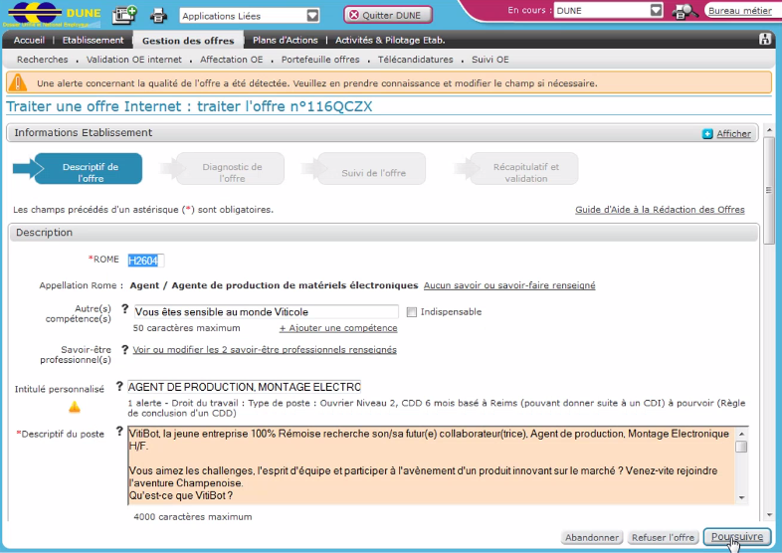
\includegraphics[width=0.9\textwidth]{S2-Explicabilite_locale/figures/Dune.png}
    \caption{Interface de l'outil de création d'offre avec une alerte liée au contrat de travail. L'alerte est accompagnée de la phrase incriminée. Le champ concerné, ``Descriptif de poste'', est surligné en jaune pour attirer l'attention de l'utilisateur. Iel peut ignorer l'alerte et cliquer sur le bouton ``poursuivre''.}
    \label{fig:ihm_DUNE}
\end{figure}

Le système actuel se concentre sur l’analyse sémantique des phrases des offres, afin de détecter un sous ensemble de motifs de non-conformité. La détection se fait au niveau des phrases d'offres d'emploi, sur le respect ou non des critères de conformité, avec 27 motifs possibles, dont le motif ``vide'' correspondant aux offres légales. Nous avons ainsi un problème de classification multi-classes. Le cas multi-label, soit le cas où une même phrase possède plusieurs motifs de rejets, correspond à moins de $1\%$ des cas. Pour simplifier, nous traiterons le cas d'usage comme un cas mono-label.

\subsection{Jeux de données} \label{C2:datasets}

Nos travaux concernent l'usage de modèles profonds tels que les réseaux de neurones. La phase d'apprentissage de ces modèles nécessite une quantité conséquente de données. Nous avons à notre disposition un large ensemble d'offres d'emploi, classées par le système historique.
Le jeu de données d'entraînement contient $480 000$ phrases extraites d'offres réelles. Une majeure partie de ces phrases sont légales : $317 843$.

La distribution des motifs de rejet présentée en figure~\ref{fig:distrib_nc} montre une répartition inégale des classes, correspondant à la répartition des données en production. Certains motifs sont extrêmement rares, tels que les rejets liés à l'ethnie : $5$ exemples sont disponibles.

\begin{figure}[htpb!]
    \centering
    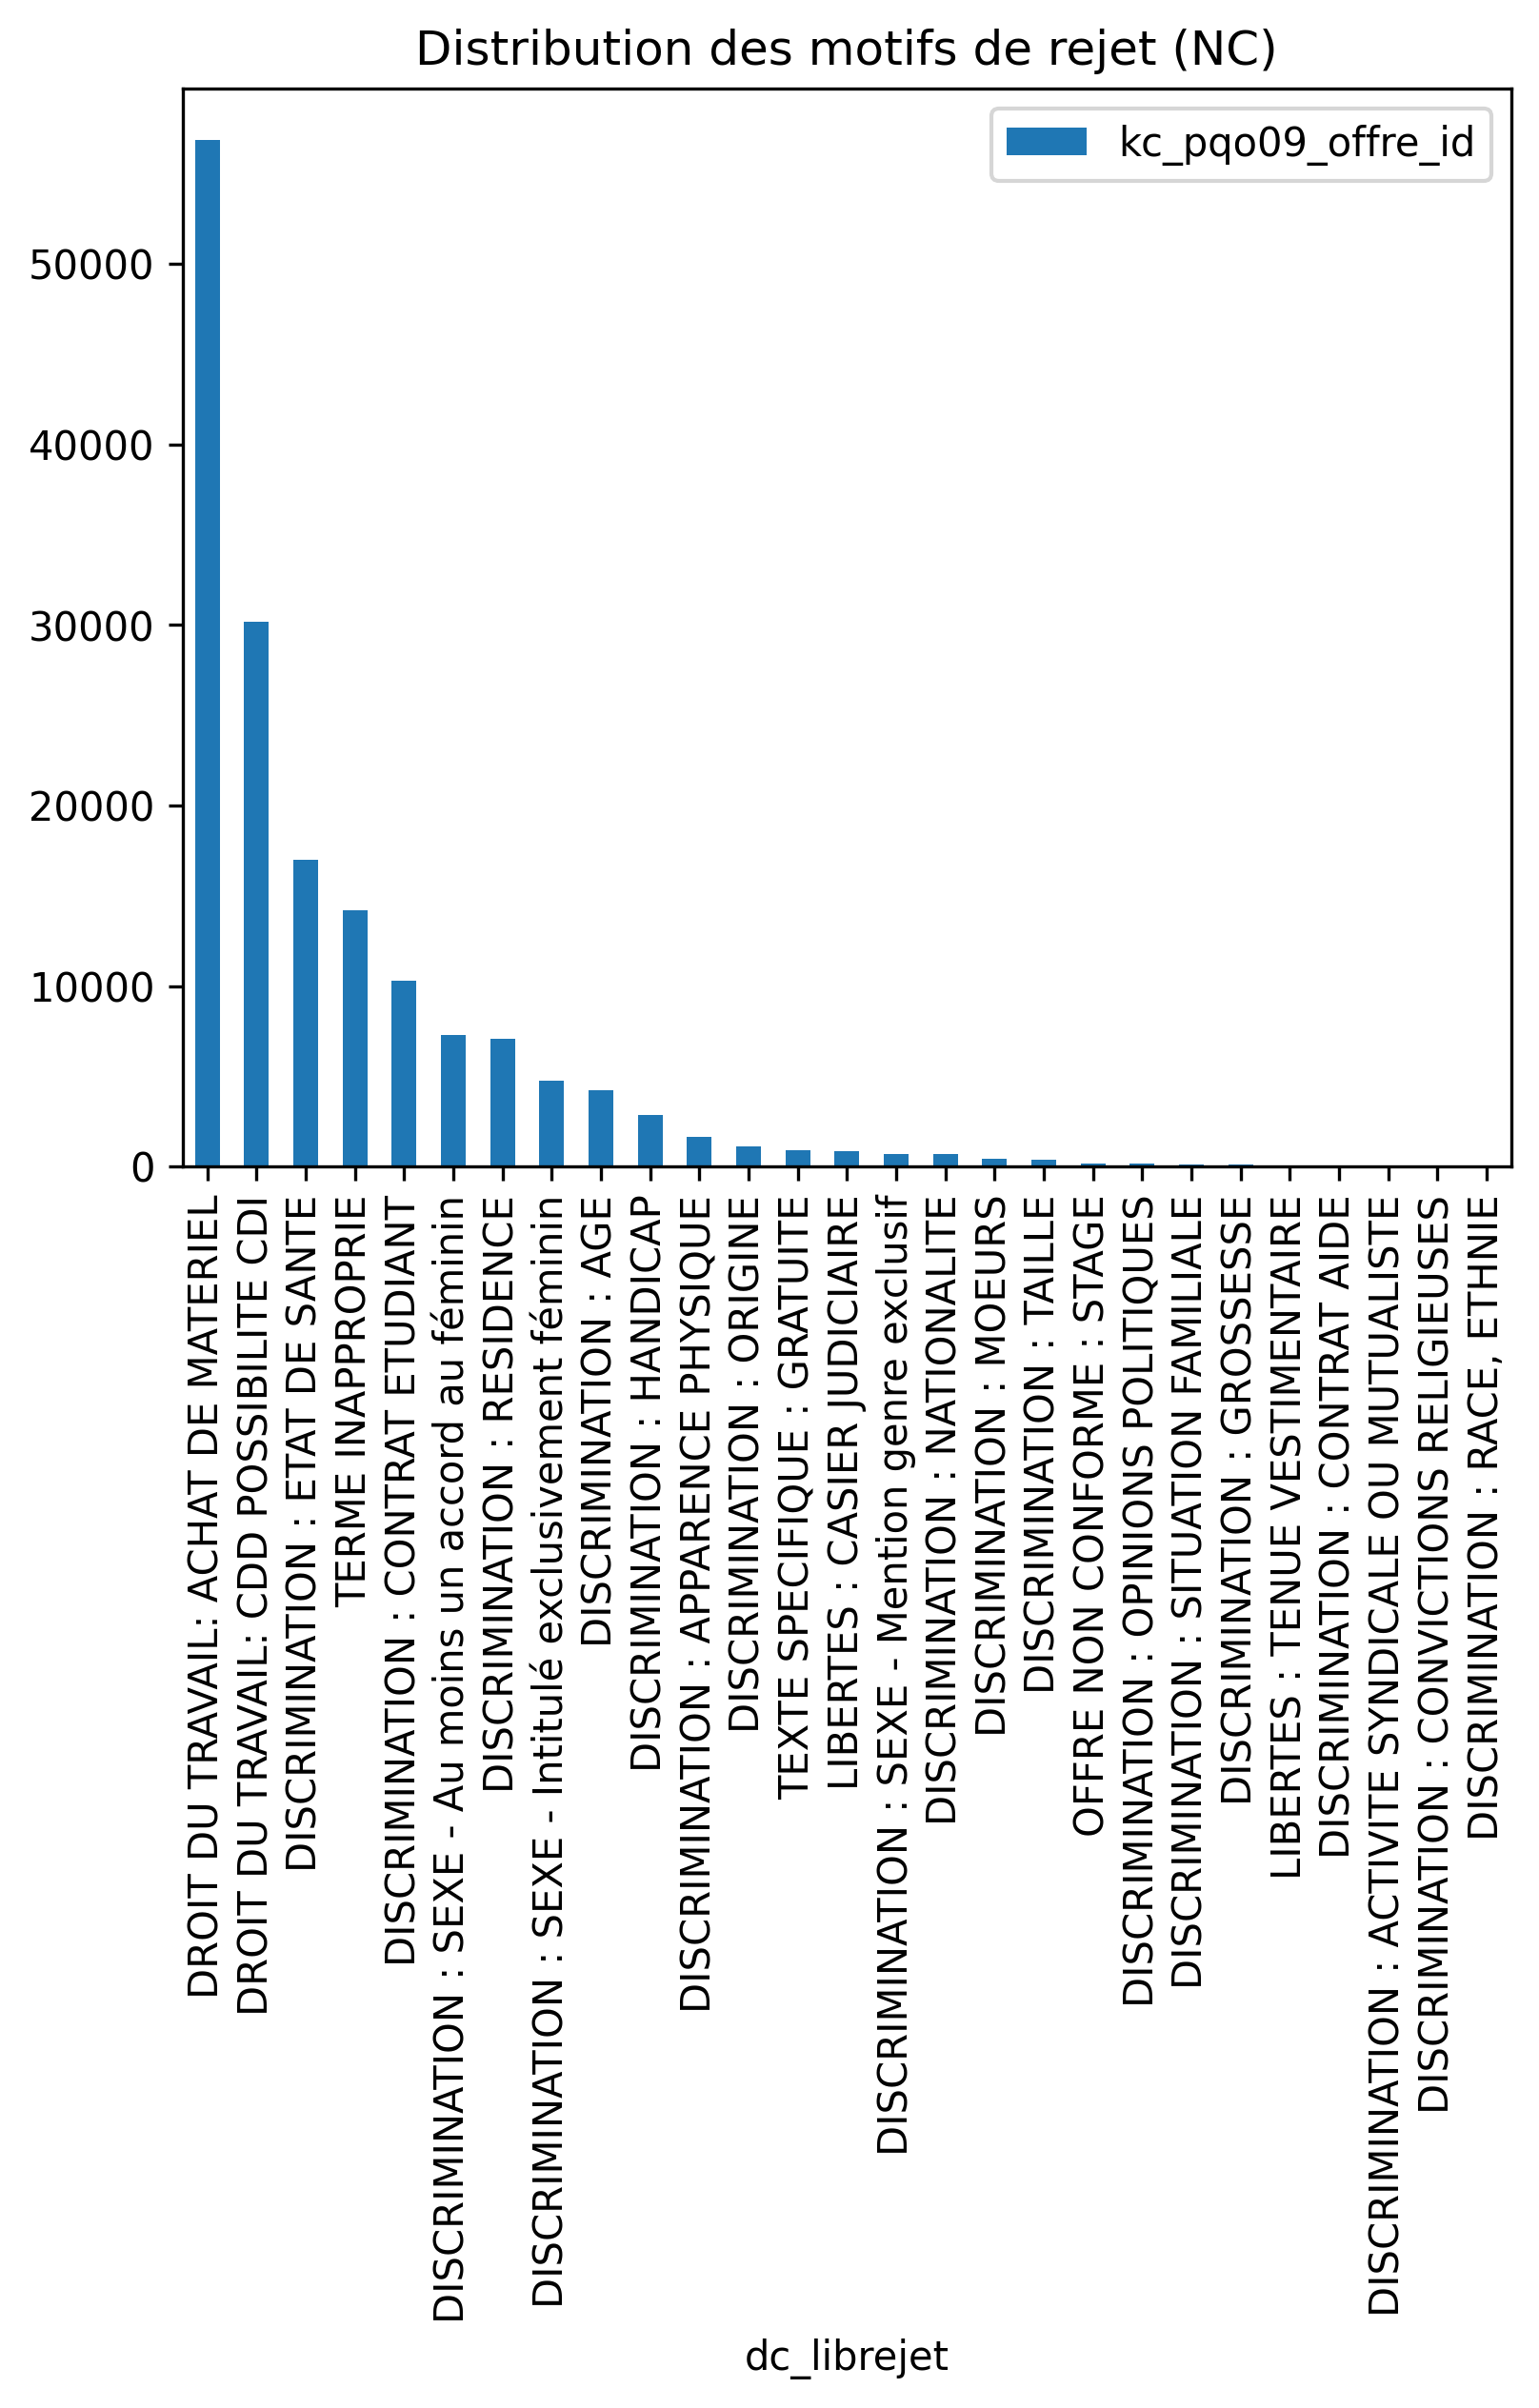
\includegraphics[width=0.8\textwidth]{./S2-Explicabilite_locale/figures/distrib_classes_NC_lego.png}
    \caption{Répartition des motifs de rejet dans les données d'apprentissage. Seules les phrases en alerte (non conformes, NC) sont prises en compte. }
    \label{fig:distrib_nc}
\end{figure}

Le jeu de données de test est constitué de données vérifiées manuellement, et les erreurs du système historiques y sont corrigées. De même, pour les phrases non conformes, les explications associées au motif de rejet sont indiquées sous forme d'ensemble de mots, à l'instar d'un surlignage. Ce travail manuel rend la création de ce jeu de données coûteux, il est donc restreint et composé de $208$ phrases uniquement.

Deux sous-échantillons de cet ensemble de test de 208 phrases sont utilisés. Le jeu de test des bonnes prédictions (BP) est composé de 147 phrases du jeu de test, correctement prédites. Ce jeu de données permet de mesurer la performance des explications lorsque le modèle ne fait aucune erreur. Cela évite que la performance des explications soit affectée dans le cas d'un modèle peu performant. L'ensemble de test de phrases avec différentes explications (DE) est composé de 106 phrases de l'ensemble de test, avec des explications non-identiques entre elles. Ce jeu de données se concentre sur la tâche des utilisateurs qui comparent les explications et évite la situation où les utilisateurs doivent choisir entre des explications uniquement identiques. Ces deux jeux de données se recoupent tel qu'illustré en figure~\ref{fig:lego_test_sets}.

\begin{figure}[htpb!]
    \centering
    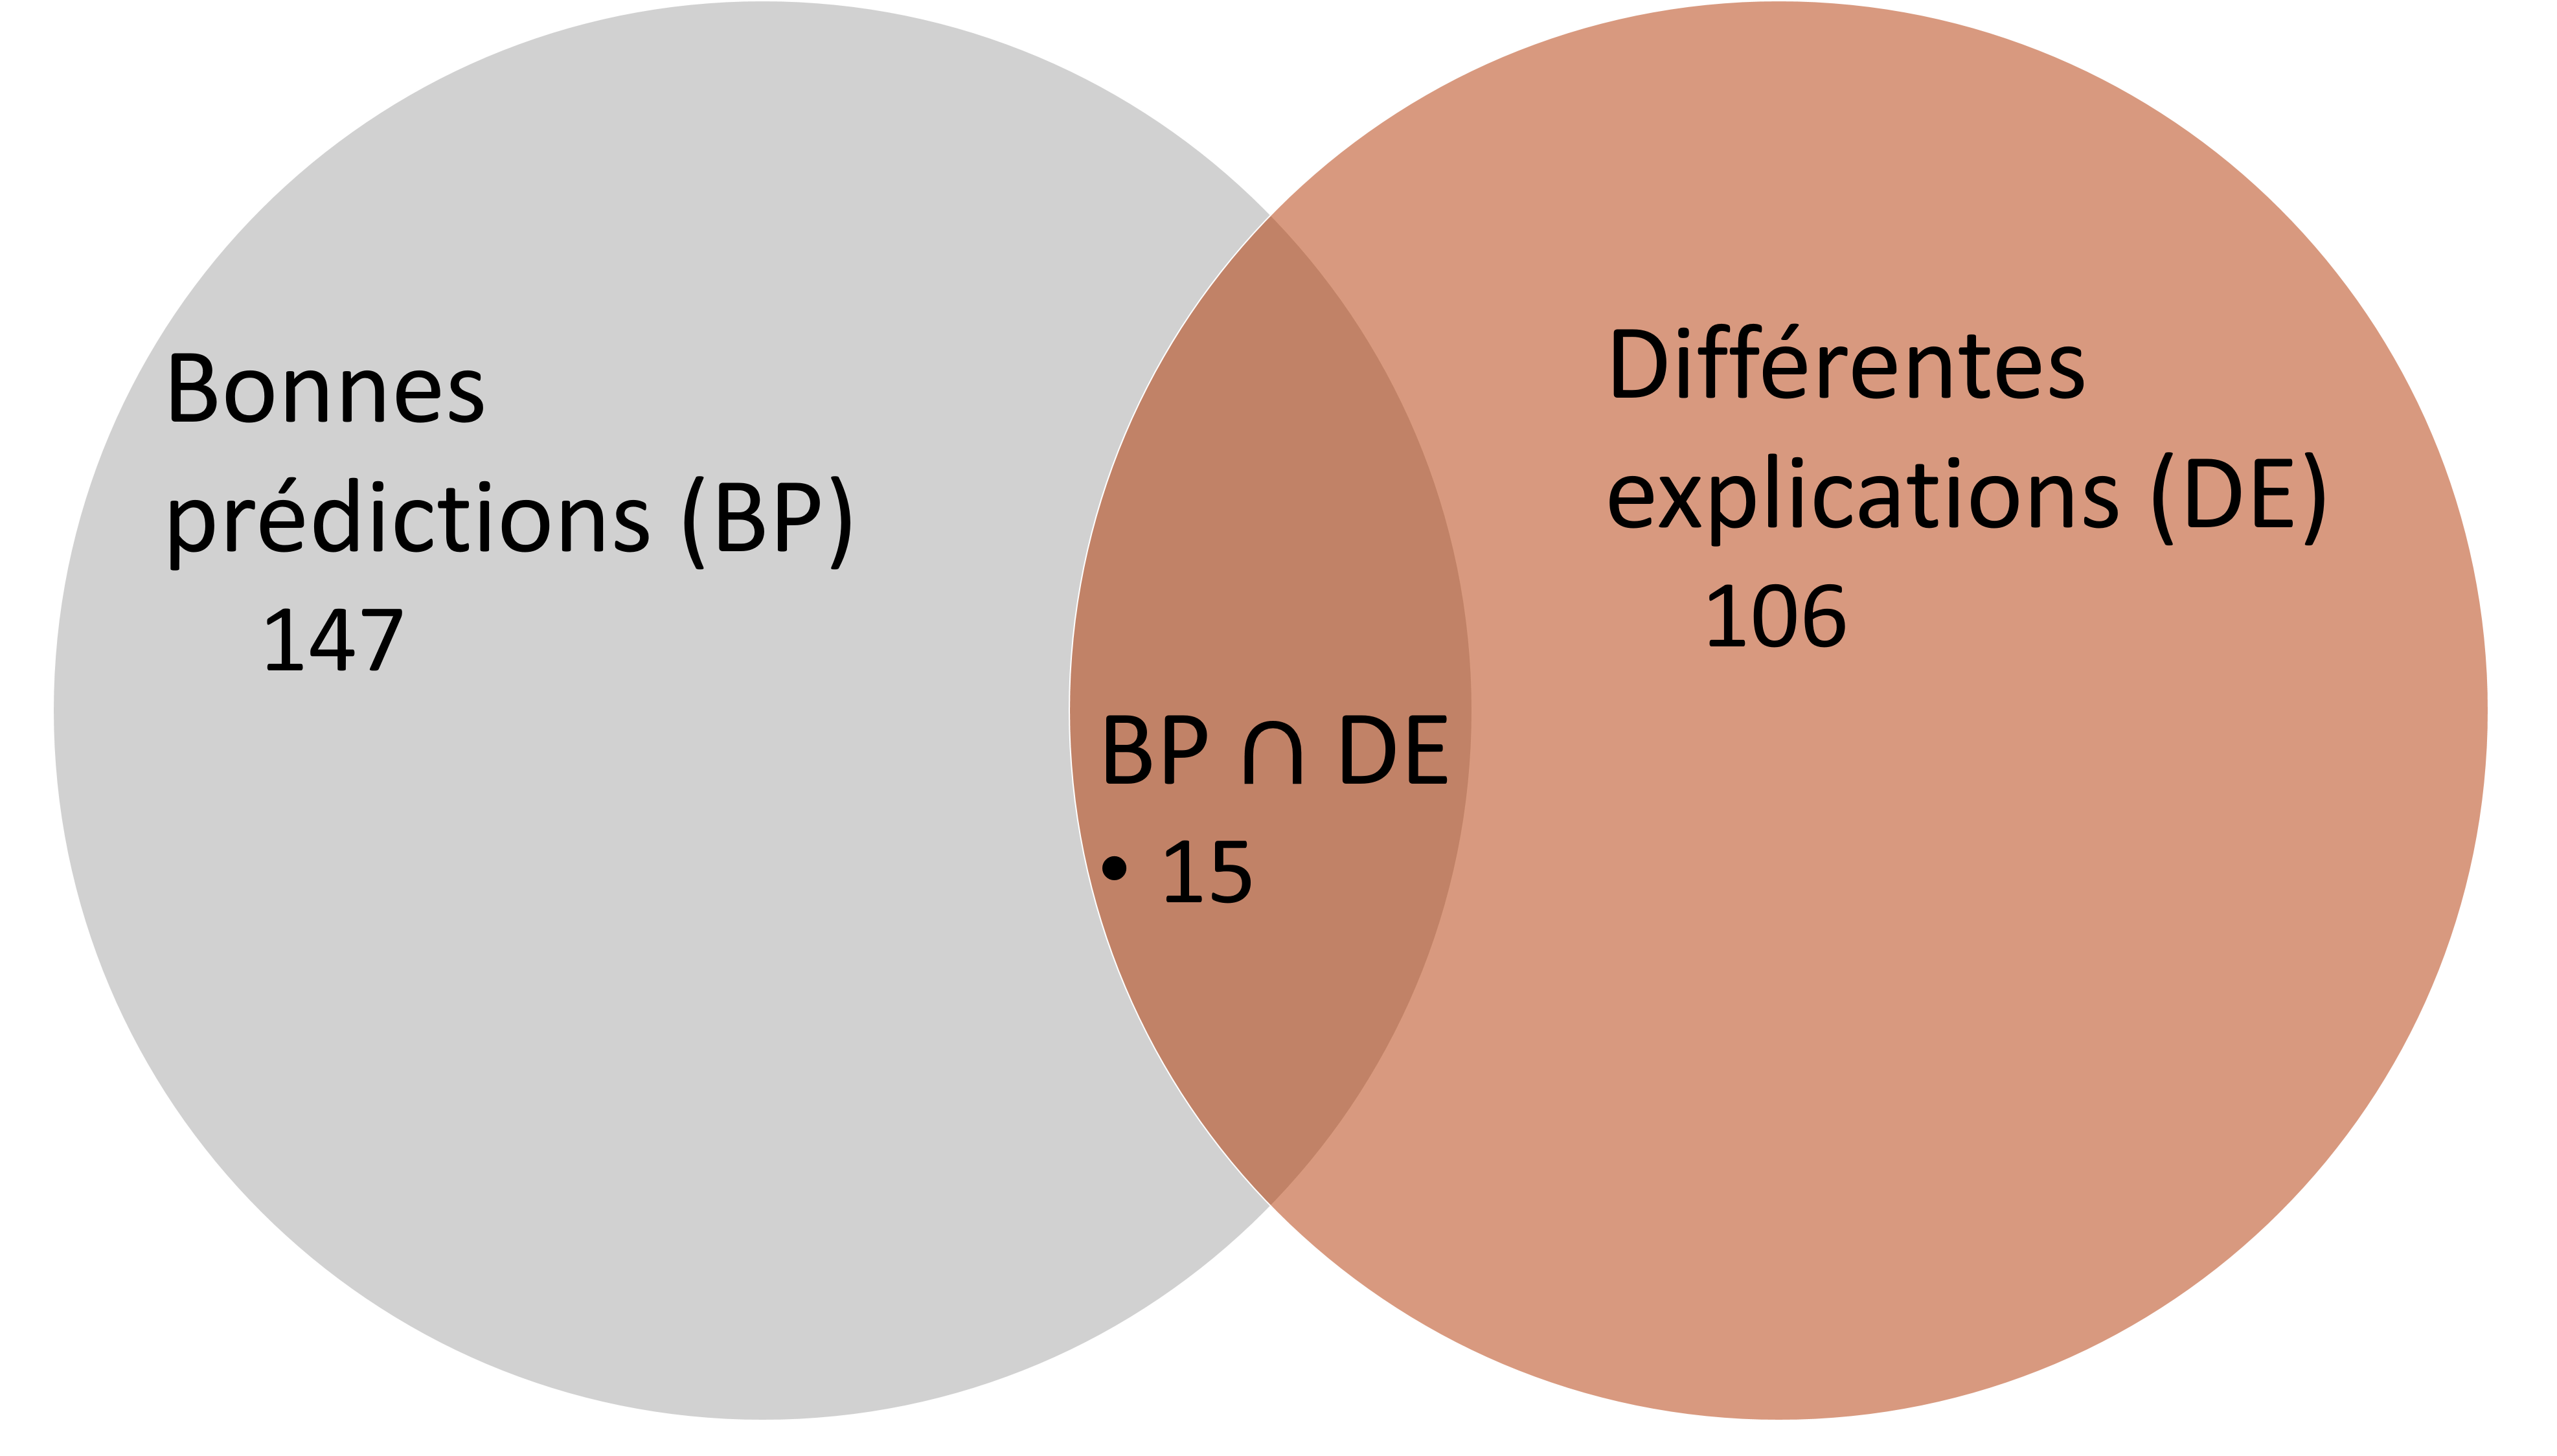
\includegraphics[width=0.6\textwidth]{./S2-Explicabilite_locale/figures/lego_test_sets.png}
    \caption{Ensemble de test de 208 phrases labellisées manuellement. Deux sous ensemble de données en sont extraits : le jeu de test de bonnes prédictions (BP) et composés de différentes explications (ED)}
    \label{fig:lego_test_sets}
\end{figure}

La création de ce jeu de test a soulevé des questionnements, tels que la difficulté de déterminer une explication idéale.

\subsection{Comment collecter les explications de référence} \label{C2:ground_truth}
Générer une explication de référence ou explication attendue peut être fait en s'appuyant sur l'attention humaine~\cite{Mohseni2021}. Il est alors nécessaire de faire appel à des experts du domaine ou, à défaut, à une documentation de référence.
On peut souhaiter obtenir une explication qui réponde à la question ``qu'est-ce qui a été utilisé par le modèle pour donner sa réponse ?''.
Pour obtenir cette explication attendue, une première technique consiste à la demander aux utilisateurs, experts du domaine ou experts du modèle.
Une seconde technique consiste à demander aux experts du domaine de vérifier les résultats des modèles et de voir où se concentre leur attention par oculométrie ou en rendant floues des parties d'une image~\cite{Das2017}. Ces méthodes sont bien adaptées aux explications basées sur les variables d'entrées. Pour des systèmes à base de règles et d'exemples, il est possible, dans un esprit similaire, de demander de rédiger l'explication, ou de la choisir parmi un ensemble pré déterminé.
% definitions
Notre objectif est de comparer les explications générées par un outil à des explications de référence. Pour une instance particulière, nous pouvons séparer les explications humaines en ``explication idéale'' et ``explication attendue''. La différence entre ces termes est définie dans les deux paragraphes suivants.

\paragraph{Une explication idéale} est une explication associée à une donnée d'entrée et sa classification correcte. Elle est idéale parce qu'elle s'applique lorsque la prédiction est juste. Cette explication est basée sur l'expertise du domaine. Si nous voulions entraîner un modèle à donner ces explications, nous les fournirions dans un jeu de données d'entraînement. Elles sont identiques, quel que soit le classifieur utilisé. Dans le cas d'une mauvaise classification, l'explication idéale ne reflète pas le comportement du modèle.

\paragraph{Une explication attendue} est une explication associée à une donnée d'entrée et une classification, que celle-ci soit correcte ou non. L'utilisateur recevant le résultat peut alors espérer obtenir une explication qui soit fidèle au raisonnement, même si erroné, du modèle.

\paragraph{Explications de référence} Nous collectons des explications de référence afin de mesurer des performances de méthode de génération d'explications, peu importe le résultat donné par le classifieur. Dans le chapitre suivant, les explications idéales sont utilisées comme référence dans les expériences réalisées.
Les experts du domaine ayant de fortes contraintes de disponibilité, nous n'avons pas de personnes expertes à disposition pour associer des phrases avec leurs explications.

\paragraph{Documentation métier} Afin de limiter les biais, nous déterminons les explications de référence grâce à la documentation métier. Cette documentation est constituée de documents techniques internes et du Guide d'Aide à la Rédaction des Offres (GARO). Le GARO est un document important pour les conseillers Pôle emploi, mais est peu pratique à utiliser lors des actes métier du fait de sa longueur : 128 pages. Ces documents nous permettent, à titre d'exemple, de déterminer que la discrimination sur le genre des candidats est détectée via l'intitulé de poste d'une offre. Cet intitulé sera alors considéré comme l'explication de référence en cas de rejet. Ces indications permettent de limiter les incertitudes dans la labellisation.

\paragraph{Spécificité du texte} Des questionnements ont émergé lors de cette phase de labellisation manuelle. Les mots porteurs de sens devaient-ils être labellisés ? Quelle est la différence entre ``Une assistante sociale'' et ``assistante sociale'' ? À des fins de simplification, nous avons fait le choix d'ignorer ces mots non porteurs de sens.

\vspace{1cm}
Nous avons défini un cas d'usage et ses données associées. Nous pouvons désormais entraîner un modèle à résoudre notre problème de classification, et générer des explications pour ce modèle.


\section{Génération d'explications par variables d'importance}\label{C2:explications}

Dans cette section, nous appliquons deux méthodes d'explication: la génération d'ancres sur n'importe quel modèle de~\cite{Ribeiro2018} et l'utilisation de l'attention avec un modèle transparent de~\cite{Lin2017}.
% pourquoi
Ce modèle fournit directement des explications locales basées sur les variables d'entrées.

Pour rappel, notre choix a été guidé par les caractéristiques suivantes:
\begin{itemize}
    \item nous ciblons les utilisateurs experts du domaine,
    \item l'explication est reçue lors de la rédaction d'une offre d'emploi,
    \item le modèle de classification est libre de toute contrainte de conception.
\end{itemize}

Nous optons pour des explications de portée locale, donnant des explications au cas par cas. La stratégie est libre, nous choisissons les deux extrêmes : modèle transparent et boîte noire. Nous appliquons deux méthodes d'explication basées sur les variables d'entrée.

Le modèle de référence sera un modèle transparent basé sur l'attention. Son avantage est de permettre la génération d'explications tout en conservant une architecture de réseau de neurone plutôt légère.
La seconde méthode choisie est une méthode boîte noire, la méthode des ancres~\cite{Ribeiro2018}. Ces travaux font suite à LIME~\cite{Ribeiro2016}, une méthode servant de référence en génération d'explications par approche boîte noire.

Les ancres seront générées sur les prédictions du modèle transparent. Ainsi, les deux explications seront basées sur le même modèle, limitant les différences entre explications aux seuls systèmes explicatifs.

En s'inspirant de~\cite{Ribeiro2018} pour l'exemple, prenons la phrase ``Ce film n'est pas mauvais'', qui est classée ``positive'' par un modèle de classification binaire de sentiments, basé sur l'attention. L'explication des ancres serait $ A = \{pas, mauvais \} \rightarrow Positive $. Chaque mot de la phrase posséderait un poids d'attention, et ``pas'' et ``mauvais'' auraient les poids les plus élevés. Les deux méthodes extraient des ensembles de mots d'intérêt. % TODO ajout formalisation sous forme d'équation

% plan
Dans un premier temps nous présenterons le modèle transparent à attention, puis nous présenterons les ancres qui permettront d'expliquer ce même modèle.

\subsection{Attention} \label{C2:attention}

% Quoi
Le mécanisme d'attention consiste à apprendre une couche spécifique d'attention à un modèle. Il est ainsi possible d'extraire des poids d'attentions associés aux variables d'entrée d'une instance, qui correspondent à une pondération de focalisation du modèle.

% comment
Suivant les recherches de~\cite{Lin2017}, nous concevons un réseau de neurones avec une architecture spécifique. Celle-ci combine un bi-LSTM, couche adaptée aux traitement de textes, et le mécanisme d'attention~\cite{Lin2017}. Les détails de l'architecture sont présentés dans le tableau ci-dessous (cf. Table~\ref{tab:model_architecture}).

\begin{table}[htb!p]
\caption{Architecture du réseau de classification à attention pour le cas d'usage LEGO.}\label{tab:model_architecture}
\begin{tabular}{|l|p{0.23\textwidth}|p{0.18\textwidth}|p{0.45\textwidth}|}
\hline
\textbf{ID} & \textbf{Type de couche} & \textbf{Paramètres} & \textbf{Commentaires} \\ \hline
1 & Couche d'entrée    & 80               & La taille est le nombre de mots dans les textes \\ \hline
2 & Plongement de mots & 300              & Plongement de mots GloVe\\ \hline
3 & Bi-LSTM            & $u=$50           & La sortie est la matrice d'états cachés H \\ \hline
4 & Couche dense 0     & $d_a=$300        & Activation $tanh$ \\ \hline
5 & Couche dense 1     & $r=$1            & La sortie est la matrice d'attention A\\ \hline
6 & Représentation     & sortie: $[2u,r]$ & Combinaison de l'attention et de la couche cachée, $M=A^T*H$ \\ \hline
7 & Sortie             &  28              & Couche de sortie \\ \hline
\end{tabular}
\end{table}

Le réseau a été adapté au cas d'usage, les dimensions des couches et autres commentaires sur l'architecture sont détaillés dans le tableau~\ref{model_architecture}. Dans ce tableau, $u$ est la taille du bi-LSTM, $d_a$ la taille de la couche dense 0, r le nombre de têtes d'attention et M la matrice de représentation. Le mécanisme d'attention aboutit à une matrice d'attention A, qui est la sortie de la couche 5 (cf. Table~\ref{model_architecture}).
L'optimisation des hyper paramètres $u$, $d_a$ a été effectuée en premier, puis le taux d'apprentissage a été ajusté sur l'intervalle $[5.10^{-5},10^{-1}]$.
Les mots d'intérêt sont filtrés en utilisant un seuil $t$ sur les valeurs d'attention. Lorsque le modèle ne prédit aucun rejet, l'explication est vide.

Pour ce classifieur, la matrice de plongement de mots utilisée est un plongement GloVe (``Global Vectors for Word Representation'') de 300 dimensions\footnote{\url{https://dl.fbaipublicfiles.com/fasttext/vectors-crawl/cc.fr.300.vec.gz}}. Le taux d'apprentissage de $0,0005$ est déterminé par essais successifs. Ce réseau atteint un taux de reconnaissance de $83,67\%$ sur son ensemble de test.

Un seuil $t$ est utilisé afin de filtrer les mots. $t$ est déterminé en optimisant l'IOU sur un ensemble de test de 208 phrases, en comparant les explications à attention et la référence. Les résultats sont présentés dans le graphique de la Figure~\ref{fig:threshold}. Ils indiquent que les mots dont l'attention est supérieure ou égale à $0,15$ constituent une bonne explication. Nous générons ainsi des explications avec les seuils de valeurs $t = 0,15$.

\begin{figure}[t]
     \setlength{\belowcaptionskip}{-20pt}
   \begin{center}
     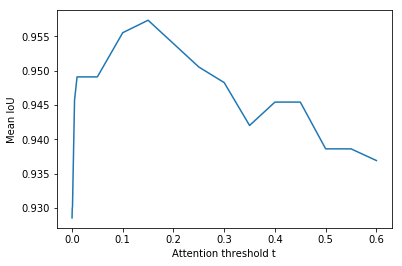
\includegraphics[height=4.5cm]{./S2-Explicabilite_locale/figures/plot_iou_threshold.png}
     \caption{Similarité (IOU) moyenne entre les explications générées et de référence dans l'ensemble de test, pour un seuil d'attention $t$ variable. Les mots dont l'attention est supérieure ou égale à $t$ forment l'explication. Le premier point est à $10^-4$. }\label{fig:threshold}
   \end{center}
\end{figure}

\paragraph{Avantages et inconvénients}
% avantages
Cette méthode de détection des mots importants a pour avantage de s'appuyer directement sur le fonctionnement interne du réseau. Le mécanisme d'attention permet de pondérer les entrées selon leur importance, avec pour objectif l'amélioration des performances du réseau. Ces pondérations sont ajustées lors de la phase d'entraînement du modèle, en optimisant les résultats de la tâche de classification. Ainsi, la génération d'explications ne nécessite pas de données supplémentaires. En faisant de l'anthropomorphisme, le réseau ``apprend de lui-même à focaliser son attention sur certains éléments''.
Le second avantage de cette méthode est qu'elle ne nécessite pas de calcul après entraînement, hormis celui de l'inférence. Plus exactement, dans l'implémentation effectuée, le modèle est appelé une fois pour obtenir le résultat, et si la phrase est rejetée, une seconde fois pour extraire les poids d'attention.

% inconvénients
Cette méthode souffre toutefois des critiques énoncées dans le Chapitre~\ref{C1}, en section~\ref{C1:debat}. Elle n'est pas toujours fiable, l'attention apprise différant parfois fortement des autres méthodes d'explicabilité, qui ont acquis leur réputation dans la communauté scientifique. Si cette méthode limite les calculs lors de l'inférence, elle nécessite tout de même d'alourdir le modèle avec les couches 4, 5 et 6 du tableau~\ref{tab:model_architecture} .


\subsection{Ancres}

% Quoi
Les ancres sont des règles extraites par analyse d'un ensemble de données générées et leurs sorties associées. Les données sont générées par perturbation de l'instance à expliquer. Les masquages permettent de déterminer quelles instances ont un impact sur le résultat final du modèle.
% comment
Nous générons les ancres avec la bibliothèque python\footnote{\url{https://github.com/marcotcr/anchor}} développée par les auteurs de~\cite{Ribeiro2018}. Afin de réduire les écarts d'explications aux seules performances des méthodes de génération des explications, les ancres sont générées en utilisant le modèle à attention développé en section~\ref{C2:attention}. Les paramètres de génération des ancres sont détaillés dans la tableau ci-dessous~\ref{tab:ancres_params}.

\begin{table}[htb!p]
\caption{Paramètre de génération des ancres pour le cas d'usage LEGO.}\label{tab:ancres_params}
\begin{tabular}{|p{0.15\textwidth}|p{0.10\textwidth}|p{0.55\textwidth}|}
\hline
\textbf{Paramètre} & \textbf{Valeur} & \textbf{Commentaires} \\ \hline
Seuil              & $0,95$ & Précision minimale requise pour ajouter un nouveau mot \\ \hline
Delta              & $0,1$  & Marge d'erreur  \\ \hline
Tau                & $0,15$ & Critère de précision de l'ancre\\ \hline
Taille de faisceau & $4$ & Taille du faisceau de recherche, sélectionne $N$ candidats à chaque tour\\ \hline
Taille de lot      & $100$  & Nombre de données générées  \\ \hline % (def. 10)
\end{tabular}
\end{table}

Dans un premier temps, rappelons quelques notations. Un domaine d'application est l'ensemble des instances pour lesquelles une règle A est vérifiée, $A(.)=1$. A est une ancre si l'ensemble $\mathbb{E}_{D(Z|A)}$ des instances du domaine d'application sont classés comme l'instance à expliquer $x$, avec un taux supérieur à la précision souhaitée $\tau$. On peut le formaliser par l'équation suivante :
\begin{equation}
     \mathbb{E}_{D(Z|A)} [ \mathbbm{1}  _{f(x)=f(z)}] \geq \tau
\end{equation}
Calculer la précision d'une ancre n'est pas possible pour un modèle $f$ et un ensemble $D$ donnés.
Nous calculons alors la probabilité que l'ancre corresponde au critère de précision $\tau$ en acceptant une marge d'erreur $\delta$.
\begin{equation}
    P(prec(A) > \tau) \geq 1 - \delta
\end{equation}

On cherche enfin à conserver les ancres qui couvrent un plus grand nombre possible d'instances. La recherche s'effectue en partant d'une ancre vide, et en créant $N$ ancres candidates par l'ajout de variables.
Les paramètres du tableau~\ref{tab:ancres_params} sont identiques aux paramètres de base des ancres. Toutefois nous avons dû augmenter la taille du faisceau de recherche, afin d'améliorer les performances.

\paragraph{Avantages et inconvénients}
% avantages
La méthode des ancres permet de générer des explications sans s'inquiéter du fonctionnement interne du modèle. Les performances de ce dernier ne sont donc pas altérées. Les explications générées ont un cadre d'application défini.

% inconvénients
Cependant cette méthode nécessite d'appeler le modèle un nombre important de fois. Elle est donc couteuse en calcul à chaque génération d'explication, et fonctionne mal sur un nombre trop important de variables d'entrées; dans notre cas, sur les phrases longues. Enfin, il y a un risque de s'appuyer sur des comportements erratiques du modèle voire de créer des instances adversariales, en définissant le comportement sur un domaine d'application constitué de données hors distribution.

\paragraph{Explications générées}
Ces deux méthodes permettent de générer différentes explications présentées dans le tableau~\ref{explications_lego}. Les explications par les ancres sont basées sur le modèle à attention, et deux explications reposent sur le mécanisme d'attention. Lorsque le modèle ne prédit aucun rejet, les explications générées sont forcées d'être vides.

\begin{table}[h!tpb]
\caption{LEGO : phrases avec leurs différentes explications. Le texte est au-dessus des autres informations. Les phrases portent respectivement les numéros 0 et 73 du jeu de données LEGO - DE.}\label{explications_lego}
\begin{tabular}{|p{0.15\textwidth}|p{0.18\textwidth}|p{0.2\textwidth}|p{0.17\textwidth}|p{0.15\textwidth}|}
  \cline{1-5}
  \textbf{Rejet} & \textbf{Référence} & \textbf{Ancres} & \textbf{Attention 0.15} & \textbf{Attention 0.5} \\ \hline
  \multicolumn{5}{|p{0.95\textwidth}|}{``[...] Notre agence de Saint-Medard-en-Jalles recherche une Assistante Administrative pour completer son equipe.''}\\ \hline
  Genre& ['assistante administrative'] & ['recherche', 'Assistante', 'Jalles'] & ['assistante', 'administrative'] & ['assistante'] \\ \cline{1-5}
  \multicolumn{5}{|p{0.95\textwidth}|}{``Poste en CDD renouvelable en cdi.''}\\ \hline
  CDD possibilit\'e CDI\footnotemark[3] & ['CDD renouvelable en cdi'] & ['CDD renouvelable', 'cdi'] & ['cdi'] & ['cdi'] \\ \cline{1-5}
\end{tabular}
\end{table}

\footnotetext[3]{Contrat à durée déterminée conduisant à un contrat à durée indéterminée}

Nous avons détaillé les méthodes de génération d'explication permettant de détecter les mots importants dans les phrases d'offres d'emploi. Dans la section suivante, nous présentons différentes interfaces d'explications pour le cas d'usage LEGO.


\section{Visualisations pour les explications locales} \label{C2:demonstrateur}

Les explications étant à destination d'humains, nous détaillons dans cette section la création d'un démonstrateur et des pistes de visualisations à présenter aux utilisateurs experts du domaine. L'objectif est de conduire un test d'utilisabilité à partir de ces visualisations pour déterminer quelles interfaces nous allons développer. Ces interfaces permettront la collecte des préférences utilisateurs.

% Quoi
Le démonstrateur est un prototype d'interface, reprenant des éléments de l'interface d'origine présentée en figure~\ref{fig:ihm_DUNE}. Dans un premier temps, nous reprenons l'interface la plus simple possible, cf. figure~\ref{fig:demo_no_exp}. Le premier élément repris est le champ de texte pour le descriptif du poste. Nous ajoutons un bouton pour lancer la prédiction, remplaçant le bouton ``poursuivre'' de l'interface d'origine.

 \begin{figure}[htpb!]
     \centering
     \begin{subfigure}[b]{0.48\textwidth}
        \centering 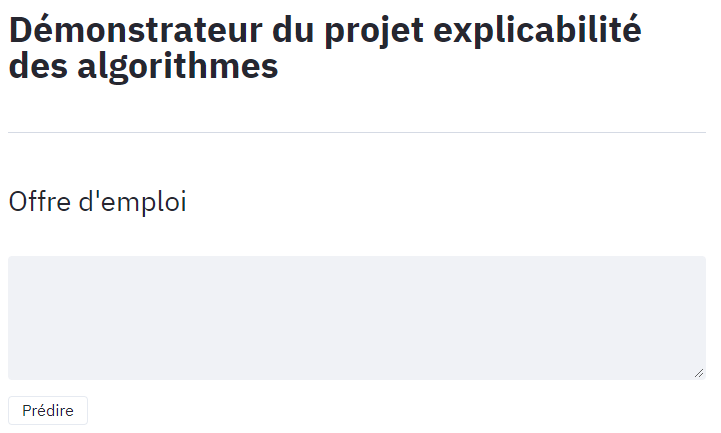
\includegraphics[width=\textwidth]{S2-Explicabilite_locale/figures/demo_empty.png}
        \caption{Démonstrateur avant prédiction}
        \label{fig:demo_empty}
     \end{subfigure}
     ~
     \begin{subfigure}[b]{0.48\textwidth}
        \centering 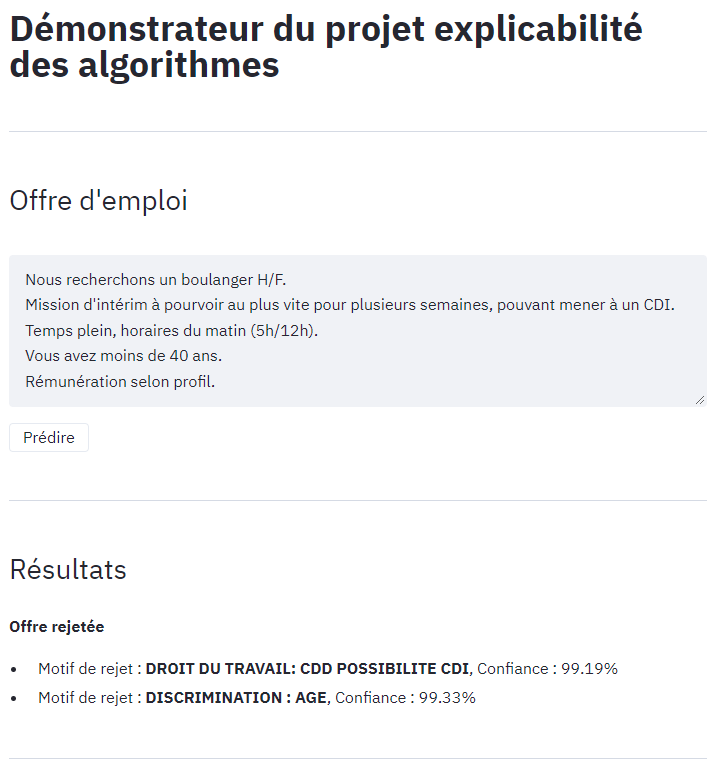
\includegraphics[width=\textwidth]{S2-Explicabilite_locale/figures/demo_base.png}
        \caption{Démonstrateur après prédiction, sans explications}
        \label{fig:demo_base}
     \end{subfigure}
     ~
     \caption{Démonstrateur présentant l'interface homme-machine du système d’explications locales, sans explications.
     }\label{fig:demo_no_exp}
 \end{figure}

% Comment
Lorsque l'utilisateur clique sur le bouton ``Prédire'', le résultat du modèle d'IA apparaît dans un encart sous le texte, présenté dans la figure~\ref{fig:demo_base}. Cette organisation diffère légèrement du bandeau explicatif situé au-dessus du texte dans l'interface d'origine en figure~\ref{fig:ihm_DUNE}, mais permet une lecture de haut en bas.
Le bandeau de résultat comprend un score de confiance du modèle. Plus le pourcentage est proche de 100\%, plus la décision est tranchée. Un score plutôt faible, vers 50\%, constitue une alerte.
Les développements se basent sur les retours du test d'utilisabilité présenté dans le chapitre suivant, en section~\ref{C3:test_u}.
Ils permettent la présentation aux utilisateurs des explications générées en section précédente, afin de collecter leurs préférences.
Nous ajoutons ensuite à ce démonstrateur différents types d'explications locales aux utilisateurs, afin de leur permettre d'interagir en se rapprochant légèrement des conditions d'usage réel, tout en restant simple à développer et maintenir. Les visualisations proposées sont une explication par surlignage de la phrase puis des mots déclenchant le rejet, d'une règle métier associée et enfin d'un contre-exemple.% Todo keep ? meh.

 % plan
Les différentes pistes envisagées sont abordées avec leurs avantages et inconvénients.
La première interface présentée est celle mettant en avant les phrases illégales. Puis vient l'explication basée sur les mots importants de cette phrase, suivie de celles basées sur les règles métiers, et les contre-exemples.

\subsection{Préparation des illustrations} \label{C2:preparation}

La préparation des illustrations est la première étape pour réaliser le test d'utilisabilité. Elles sont réalisées eu égard aux préoccupations du public cible; les experts du domaine. Ces objectifs sont les suivants :
\begin{itemize}
    \item corriger une offre rejetée,
    \item détecter si l’outil se trompe,
    \item créer de la confiance en l'outil.
\end{itemize}

Les illustrations prennent en compte différents éléments de l'interface d'origine, présentée dans le chapitre 2. À savoir le bandeau d'alerte, la raison de l'alerte et le champ de descriptif du poste.
Nous reprenons ces éléments et les repositionnons dans les illustrations, en partant sur quatre pistes, à savoir la mise en avant d'une phrase, d'un mot, d'un exemple et d'un contre-exemple. Chaque piste est illustrée et détaillée dans les paragraphes ci-après.

\paragraph{Illustration d'explication par phrase}
% Quoi
La première proposition d'illustration est la mise en avant de la ou les phrases entraînant le rejet d'une offre.
% Pourquoi
Elle permet de donner le contexte du rejet, le texte étant analysé phrase par phrase. L'explication est donc à son niveau de contexte le plus large, laissant au receveur de l'explication le soin de comprendre le détail.
% variantes
Pour mettre en avant une phrase, de nombreuses options sont possibles. Nous en avons prédéterminé trois, présentées dans la figure~\ref{fig:prototype_phrase}.
Il est ainsi possible de la surligner pour indiquer son rejet, comme dans la figure~\ref{fig:prototype_phrase1}.
De même, pour faire apparaître plusieurs éventuels motifs de rejet pour une même phrase, nous pouvons la souligner comme présenté dans la figure~\ref{fig:prototype_phrase2}.
Enfin, une autre proposition est d'afficher une bulle explicative lorsque le curseur de l'utilisateur survole la phrase, idée schématisée dans l'illustration en figure~\ref{fig:prototype_phrase3}.

% illustration
\begin{figure}[htpb!]
    \centering
    \begin{subfigure}[b]{\textwidth}
        \centering 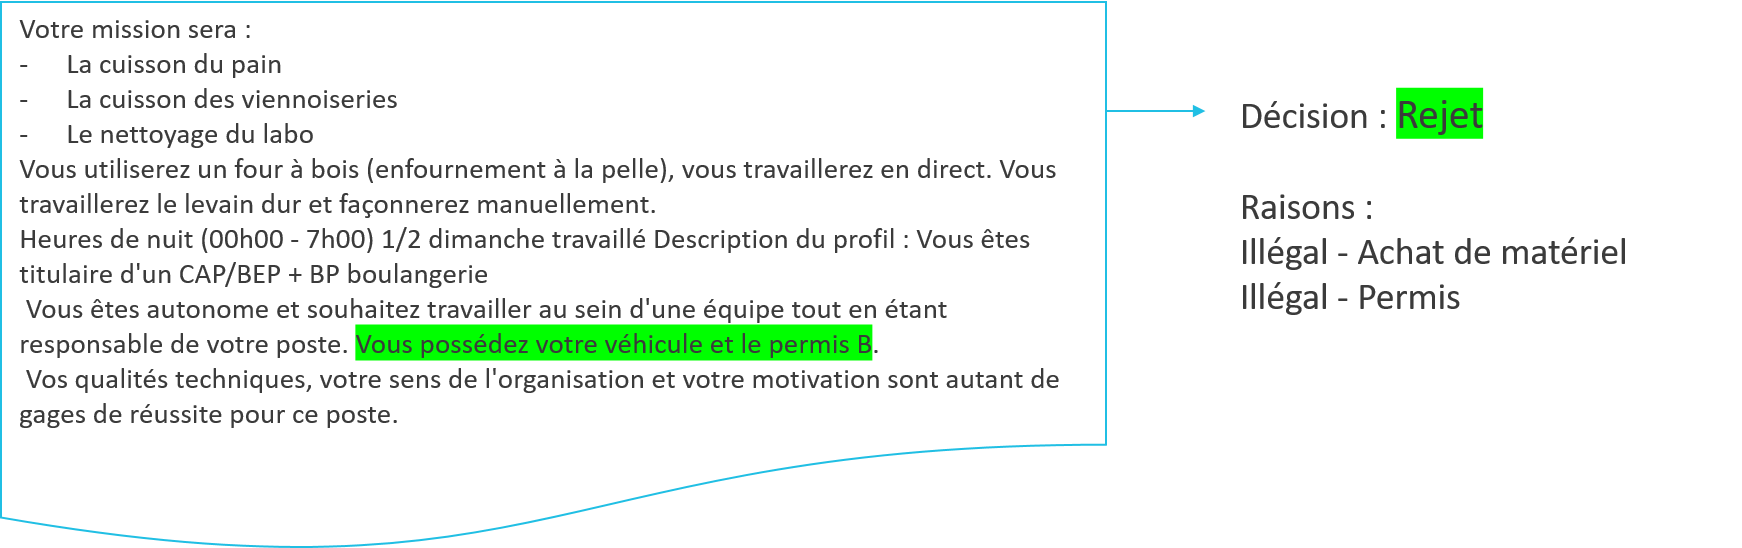
\includegraphics[width=\textwidth]{S2-Explicabilite_locale/figures/prototype_phrase1.png}
        \caption{Mise en avant d'une phrase rejetée par surlignage}
        \label{fig:prototype_phrase1}
    \end{subfigure}
    ~
    \begin{subfigure}[b]{\textwidth}
        \centering 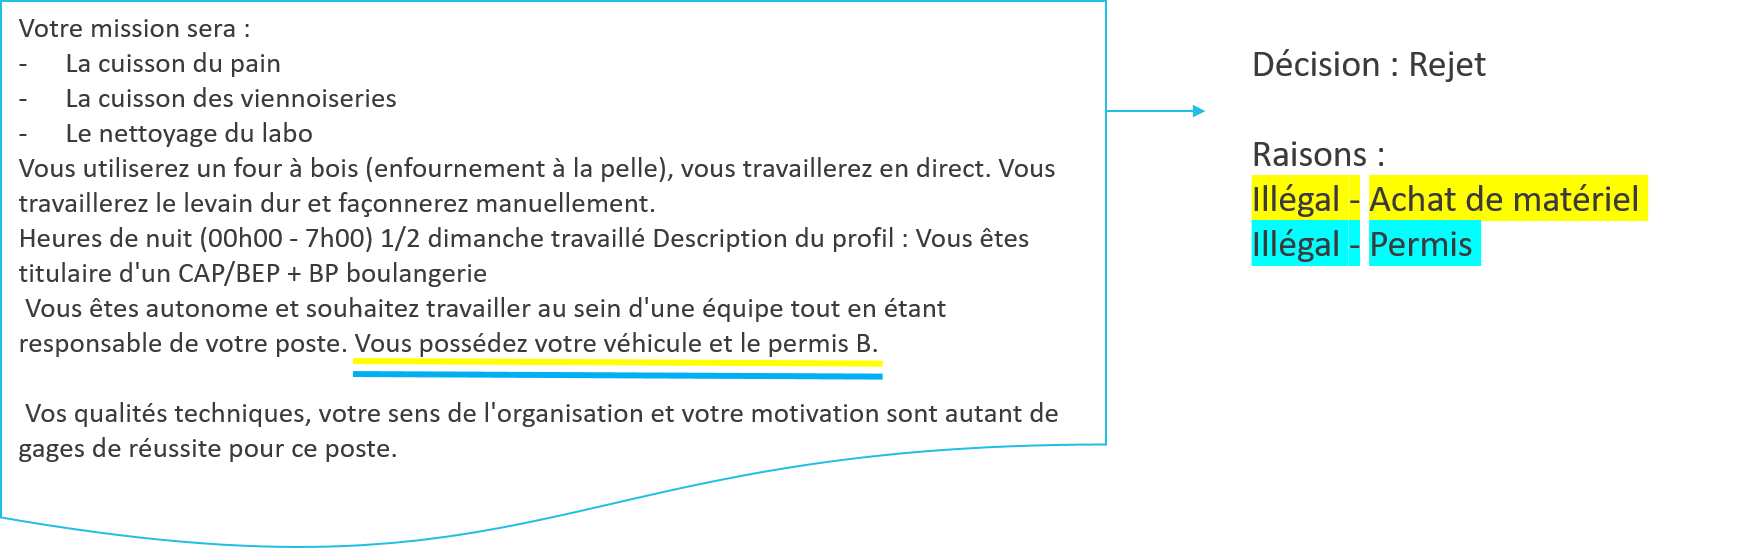
\includegraphics[width=\textwidth]{S2-Explicabilite_locale/figures/prototype_phrase2.png}
        \caption{Mise en avant d'une phrase rejetée par soulignage}
        \label{fig:prototype_phrase2}
    \end{subfigure}
    ~
    \begin{subfigure}[b]{\textwidth}
        \centering 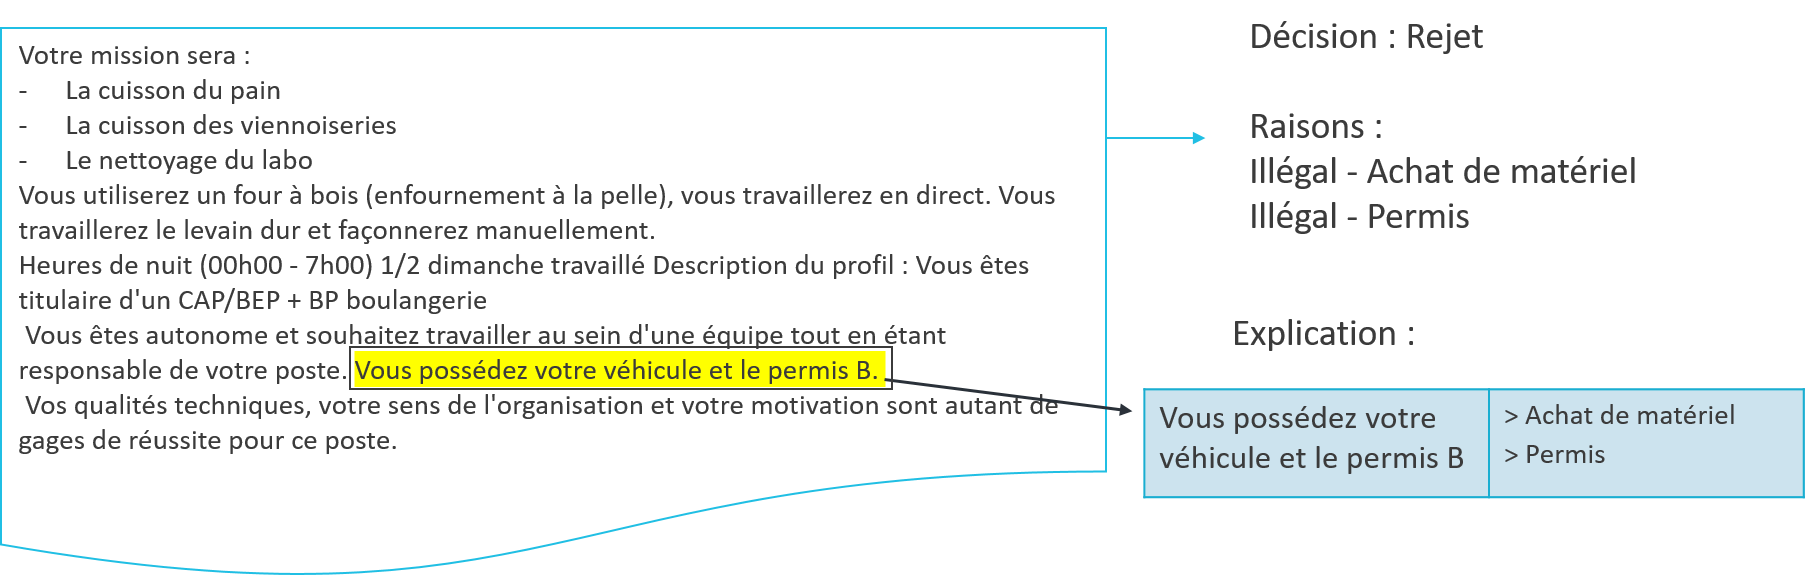
\includegraphics[width=\textwidth]{S2-Explicabilite_locale/figures/prototype_phrase3.png}
        \caption{Mise en avant d'une phrase rejetée via surlignage et bulle d'information apparaissant au survol de la phrase}
        \label{fig:prototype_phrase3}
    \end{subfigure}
    ~
    \caption{Illustrations de variantes d'une explication par la mise en avant d'une phrase.
    }\label{fig:prototype_phrase}
\end{figure}

\paragraph{Illustration d'explication par mot}
 % Quoi
 La seconde proposition consiste à mettre en avant les mots de la phrase responsables du rejet.
 % Pourquoi
 C'est l'explication avec le plus de précision, les phrases étant parfois longues. En contrepartie c'est l'explication qui donne le moins de contexte. Elle est également très proche du système expert d'origine, celui-ci étant basé sur des expressions régulières. Ce système original remontait donc des mots ou ensemble de mots prédéterminés et consignés dans un cahier des charges, sans tenir compte du contexte.
 % variantes
 Similairement aux phrases, nous proposons différentes variantes de maquette. Ces variantes sont illustrées dans la figure~\ref{fig:prototype_mot}. La figure~\ref{fig:prototype_mot1} montre les mots soulignés. Les mots peuvent être surlignés, avec une bulle indiquant le motif de rejet affiché au survol du mot en question, comme illustré en figure~\ref{fig:prototype_mot2}. Enfin, pour se rapprocher de l'interface d'origine, il est également proposé d'afficher le ou les mots en questions en dehors du champ texte, dans un bandeau à part. Cette maquette est illustrée en figure~\ref{fig:prototype_mot3}.
 % illustration
 \begin{figure}[htpb!]
     \centering
     \begin{subfigure}[b]{\textwidth}
        \centering 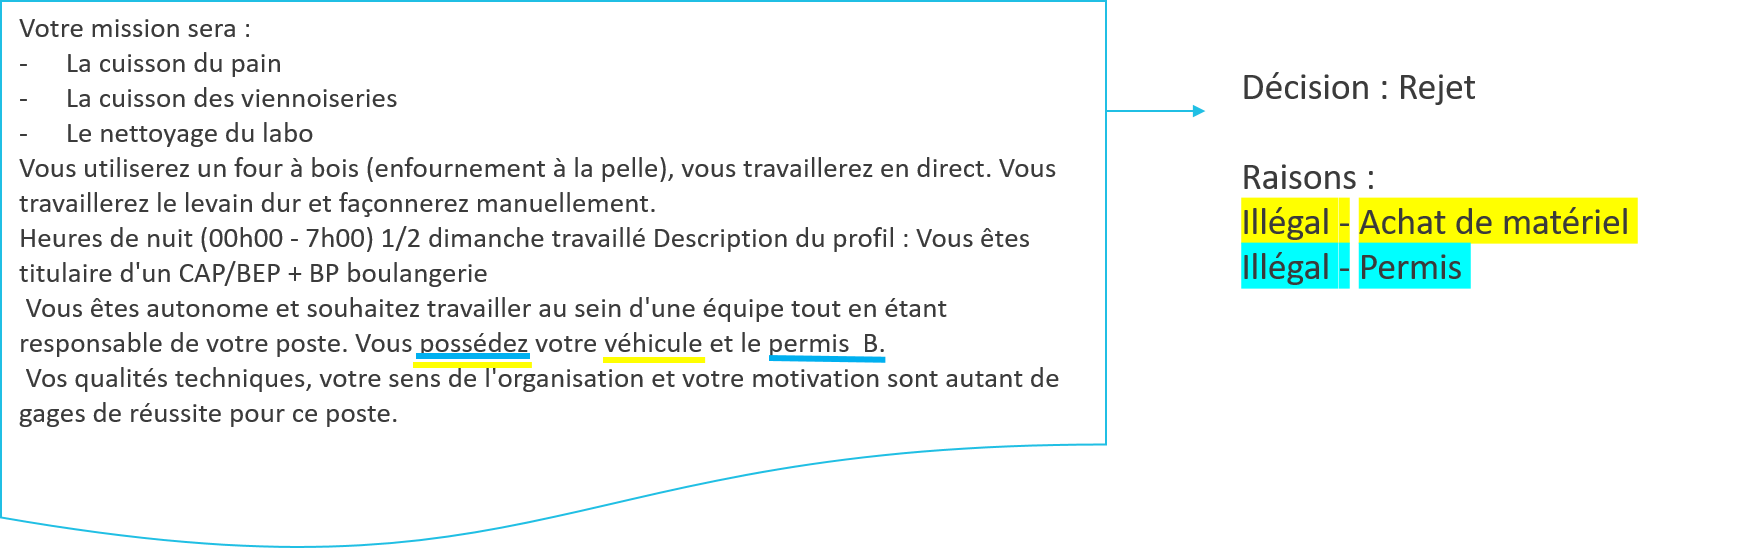
\includegraphics[width=\textwidth]{S2-Explicabilite_locale/figures/prototype_mot1.png}
        \caption{Mise en avant de mots par soulignage}
        \label{fig:prototype_mot1}
     \end{subfigure}
     ~
     \begin{subfigure}[b]{\textwidth}
        \centering 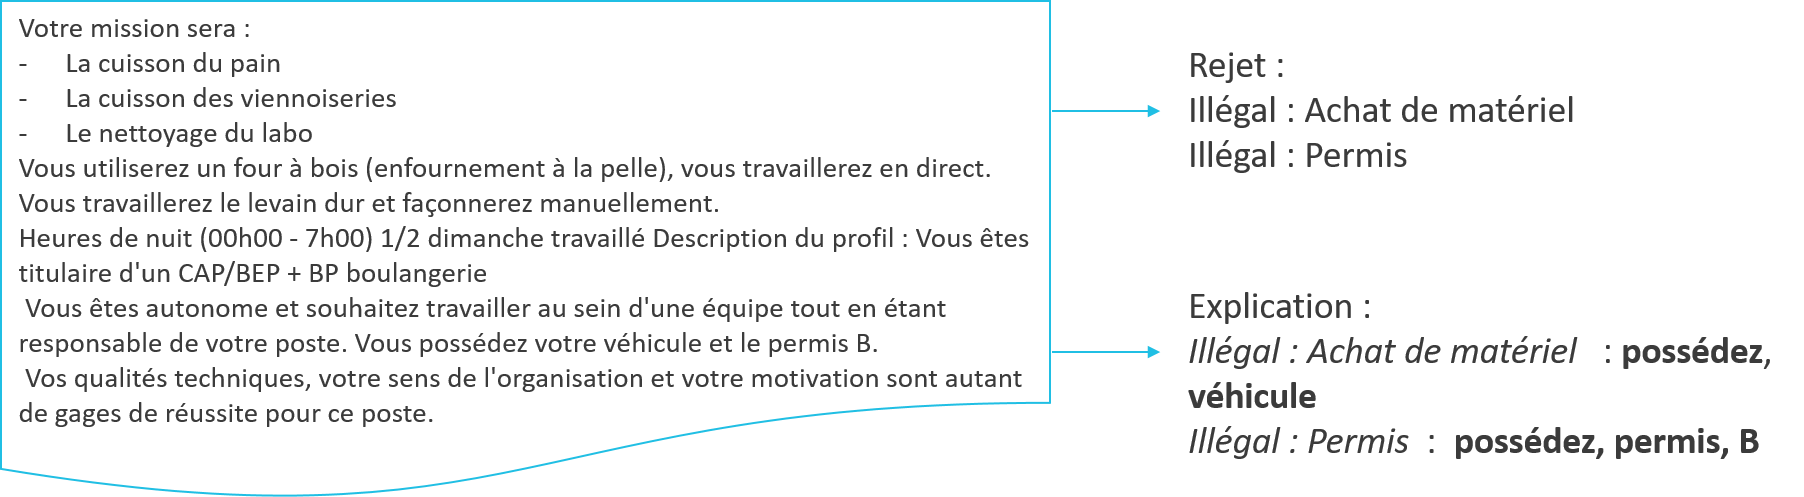
\includegraphics[width=\textwidth]{S2-Explicabilite_locale/figures/prototype_mot3.png}
        \caption{Mise en avant de mots par affichage dans un bandeau externe}
        \label{fig:prototype_mot2}
     \end{subfigure}
     ~
     \begin{subfigure}[b]{\textwidth}
        \centering 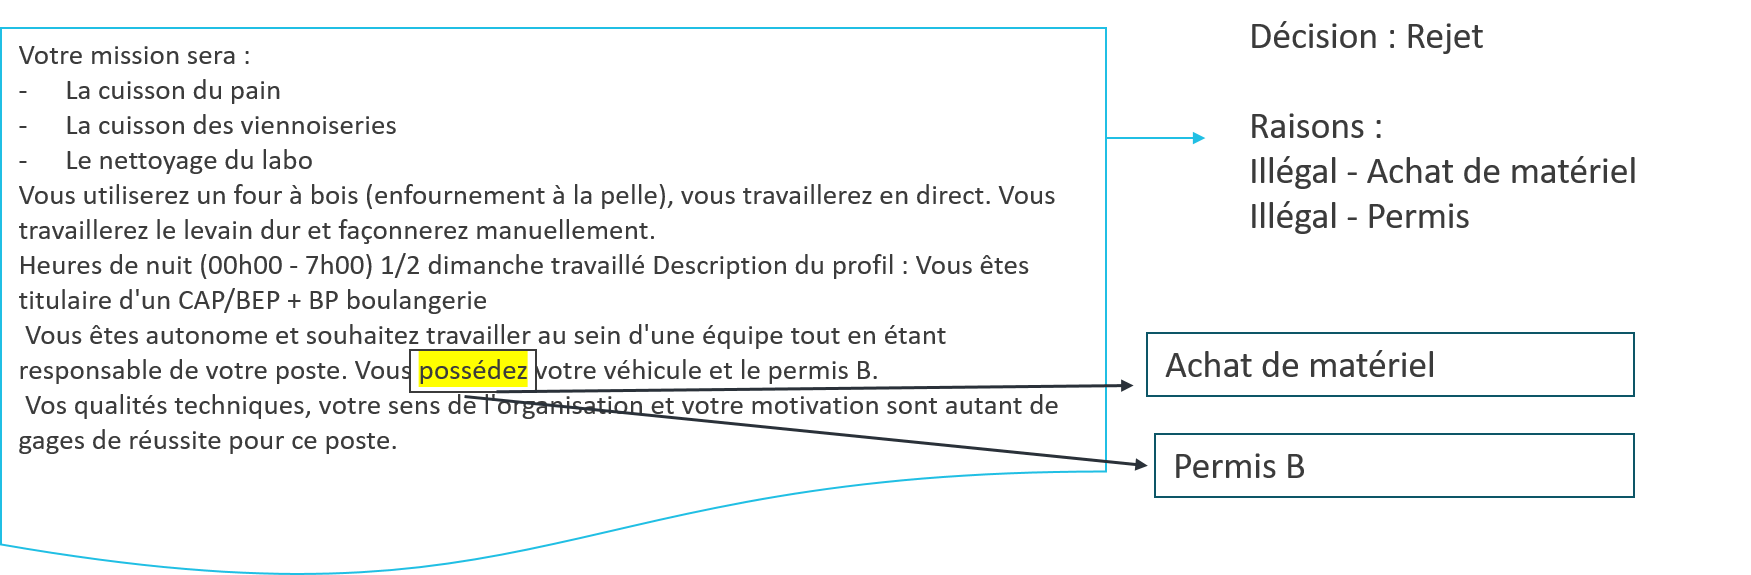
\includegraphics[width=\textwidth]{S2-Explicabilite_locale/figures/prototype_mot2.png}
        \caption{Mise en avant de mots via surlignage et bulle d'information apparaissant au survol des mots}
        \label{fig:prototype_mot3}
     \end{subfigure}
     ~
     \caption{Illustrations de variantes d'une explication par la mise en avant de mots.
     }\label{fig:prototype_mot}
 \end{figure}

\paragraph{Illustration d'un exemple}
 % Quoi
 La troisième maquette proposée est l'explication par l'exemple, affichant pour chaque phrase rejetée une phrase proche, elle aussi classée sur le même motif de rejet.
 % Pourquoi
 Ce type d'explication permet à l'utilisateur d'avoir un exemple de phrase qui entraîne un rejet, et qui comportera sans doute des mots identiques ou similaires à la phrase responsables du rejet. La figure~\ref{fig:prototype_exemple} présente l'illustration proposée, avec une phrase proposée pour chaque motif de rejet détecté.
 % illustration
 \begin{figure}[htpb!]
     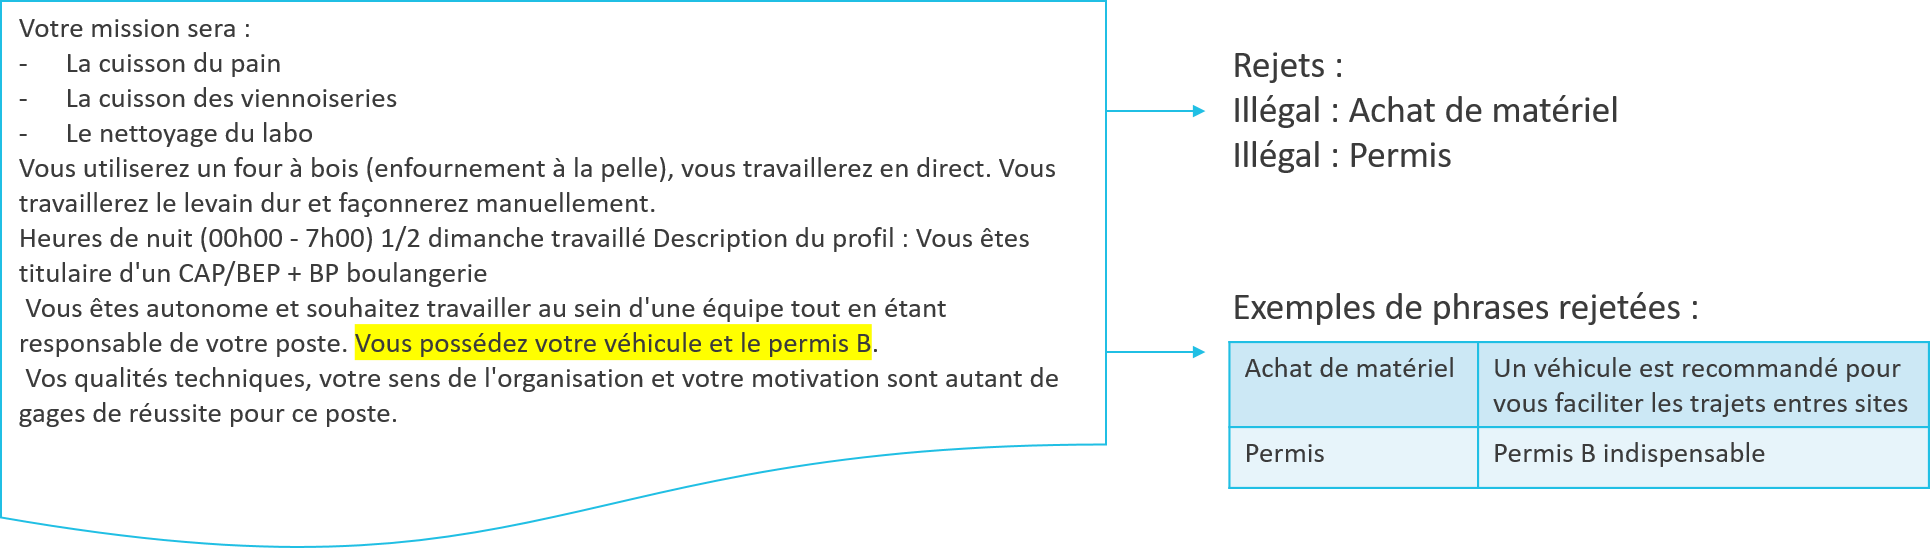
\includegraphics[width=\textwidth]{./S2-Explicabilite_locale/figures/prototype_exemple.png}
     \caption{Illustration d'explication par l'exemple}
     \label{fig:prototype_exemple}
 \end{figure}

\paragraph{Illustration d'un contre-exemple}
 % Quoi
 Enfin, la dernière maquette que nous proposons est l'explication par le contre-exemple, affichant pour chaque phrase rejetée une phrase proche, mais cette fois qui n'est pas rejetée par le système.
 % Pourquoi
 Ce type d'explication permet à l'utilisateur d'avoir un exemple de phrase acceptée, tout en étant proche sémantiquement de la phrase entraînant un rejet. Les contre-exemples sont illustrés en figure~\ref{fig:prototype_contre_exemple} avec comme précédemment une phrase par motif de rejet détecté.
 % illustration
 \begin{figure}[htpb!]
     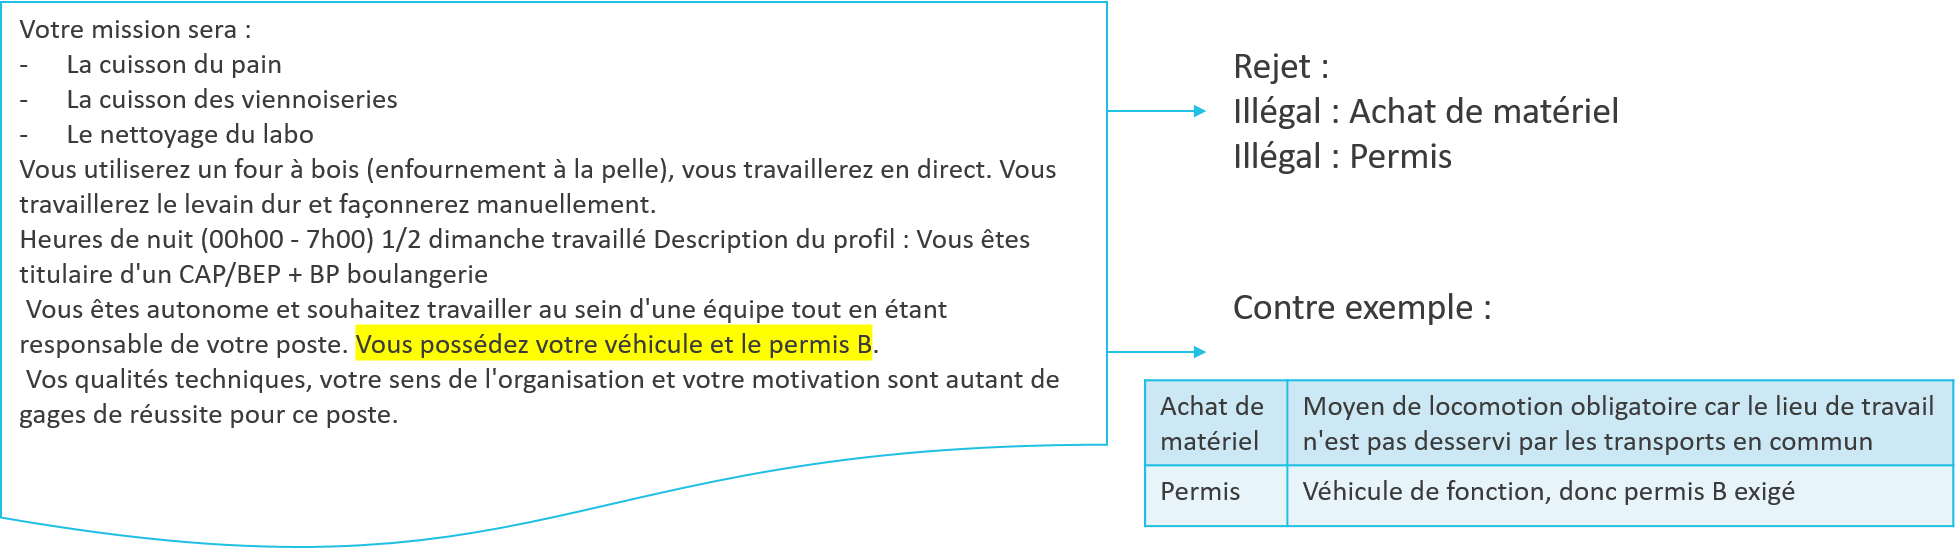
\includegraphics[width=\textwidth]{./S2-Explicabilite_locale/figures/prototype_contre_exemple.png}
     \caption{Illustration d'explication par le contre-exemple}
     \label{fig:prototype_contre_exemple}
 \end{figure}

Toutes ces illustrations sont présentées aux personnes participant au test d'utilisabilité, présenté dans le chapitre suivant.

\section{Conclusion}

% Objectif du chapitre
Dans ce chapitre, nous avons présenté le contexte applicatif de nos travaux, et les pré-requis à la réalisation de ceux-ci. Le cas d'usage illustrant nos travaux est développé en section~\ref{C2:usecase}. Nous avons généré des explications en section~\ref{C2:explications}, et préparé diverses illustrations section~\ref{C2:demonstrateur}.

% on en retire quoi, limites
La labellisation manuelle des données a mis en évidence des problématiques liées à la nature des données, avec la question de la prise en compte des mots vides de sens. La recherche d'une explication idéale qui corresponde aux préférences des utilisateurs est cruciale. Elle passe par la concertation des experts, mais également un travail de terrain coûteux de collecte d'une quantité significative d'explications, permettant d'obtenir un consensus.

Le temps limité de la thèse a amené à la labellisation d'une quantité restreinte de données. L'expérience ainsi acquise pointe vers la nécessité d'une définition collégiale des explications de référence. Avec une telle définition, il devient intéressant de collecter une quantité importante d'explications.

% Et la suite ?
Nous avons généré des explications, collecté des préférences et déterminé des explications faisant office de référence. Dans le prochain chapitre nous allons déterminer comment comparer des méthodes d'explicabilité, sur la forme et le fond.

\boitemagique{Résumé}{
\begin{itemize}
    \item[\checkmark] Nous avons labellisé un ensemble de données de test
    \item[\checkmark] La définition d'une explication de référence de qualité n'est pas une évidence
    \item[\checkmark] Nous avons généré des explications par mots importants
    \item[\checkmark] Nous avons proposé différentes visualisation d'explications locales
\end{itemize}
}


\clearemptydoublepage
\chapter[Comparaison d'explications locales]{Comparaison d'explications locales} \label{C3}

\boitemagique{Dans ce chapitre}{
    Nous traitons ici l'évaluation des explications. Trois protocoles sont proposés, afin d'évaluer le format et la méthode de génération des explications.
    L'application des différents protocoles met en avant leurs intérêts et limites.
    Les protocoles d'évaluation des méthodes de génération présentent une forte dépendance à la disponibilité d'une explication de référence de qualité.
}

% Quoi
Dans le chapitre précédent, nous avons conçu différentes illustrations d'explications, et appliqué plusieurs méthodes de générations d'explications pour un même format. Nous allons maintenant mettre en place des protocoles de comparaison de ces formats et méthodes, avec et sans utilisateurs.
L'application des protocoles montre leurs intérêts et limites respectives, notamment liées à la qualité des explications de référence.

% Plan
La collecte des retours utilisateurs est présenté en section~\ref{C3:test_u}. Nous recueillons les avis d'experts sur différentes illustrations, et nous développons des interfaces en conséquence. Enfin, nous présentons la collecte des préférences des experts du domaine.
Dans la section~\ref{C3:iou_expe} les méthodes sont comparées en se basant sur des métriques objectives, permettant de valider le respect de critères donnés. Cette expérimentation se fait sans utilisateurs.
Elle peut être menée rapidement et nécessite peu de prérequis.
Dans la section~\ref{C3:pus}, les utilisateurs cible sont intégrés à l'expérimentation, permettant de mesurer leurs préférences. Cette expérimentation nous permet de questionner la qualité des explications de références et la pertinence de la mesure utilisée en section~\ref{C3:iou_expe}.

\section{Collecte des retours des experts} \label{C3:test_u}
% quoi
Dans un premier temps nous présentons les collectes des retours des utilisateurs experts du cas d'usage LEGO.
% plan
En section~\ref{C3:discussion} nous présentons les analyses à chaud et discussions avec le panel d'experts autour des illustrations du chapitre 2.
Nous détaillons les interfaces créées grâce à ces retours en section~\ref{C3:solution} en précisant quelles solutions sont écartées, retenues, et quelles adaptations sont prises en compte.
En section~\ref{C2:collect_pref} nous présentons la collecte de préférences utilisateurs réalisée à partir de l'interface développée en section~\ref{C3:solution}.

\subsection{Test d'utilisabilité}\label{C3:discussion}

Le point avec les experts débute par plusieurs rappels permettant de s'assurer que les éléments de vocabulaire, objectifs et éléments fonctionnels sont bien partagés par tous. Nous rappelons quel est l'acte métier étudié, à l'aide d'un exemple qui nous servira tout au long de la présentation. Cela nous permet de dé-corréler l'analyse de l'interface de l'analyse métier. La discussion est basée sur les illustrations présentées en chapitre 2.

% Qui
% KAZBENNAOU Brahim - chargé relation entreprises - missionné DSI
% LECORBEILLER Eric - Manager de terrain
% PHAROSE Samuel & MAILHOL Sandrine - conseillers E
Les personnes identifiées pour ce test sont toutes expertes dans l'analyse de la qualité des offres d'emploi. Elles sont quatre, de métiers complémentaires. Ce panel est ainsi constitué d'un chargé de relations entreprises, un manager de terrain, et un conseiller et une conseillère à dominante entreprise.

Une fois les illustrations présentées, les experts donnent leurs avis sur chacune des propositions, discutent entre eux et mettent en avant les éléments qui leur manquent.
L'objectif de cette phase de discussion est de faire le tri sur les propositions et leurs variantes, ajuster les maquettes au besoin des personnes interrogées, et palier aux éventuels oublis et manques.
Nous passons en revue chaque proposition et les nouvelles idées sont traitées à part.

\paragraph{Explication par phrase} La mise en avant de phrases a été très appréciée par le panel d'utilisateurs. Iels apprécient le contexte global que fournit la phrase entière, notamment lorsque le descriptif de l'offre est long.
Parmi les variantes, le surlignage est bien perçu tandis que le soulignage n'est pas apprécié. La bulle d'informations au survol de la phrase est fortement rejetée.

\paragraph{Explication par mot} La mise en avant de mots a été bien reçue par les utilisateurs. Le système précédent fournissant des mots ou expressions également, cette solution ressemble fortement à ce qu'iels connaissent déjà, réduisant ainsi le cout de changement. Comme pour les phrases, la variante de surlignage des mots est plébiscitée, et les bulles lors du survol sont fortement rejetées. Les utilisateurs préfèrent le surlignage dans le texte plutôt que le bandeau à part. Si ce bandeau correspond à l'interface actuelle de DUNE (cf. figure~\ref{fig:ihm_DUNE}), le surlignage direct réduit les allers-retours visuels.

\paragraph{Exemple} L'explication par l'exemple n'a pas convaincu les utilisateurs. Iels ne voient pas l'intérêt de montrer une phrase proche et toujours rejetée, car cette phrase ne donne pas d'information intéressante. Les éléments communs pourraient être détectés par le surlignage de mots et le contexte global pourrait être mis en avant en surlignant la phrase rejetée. L'exemple ajoute de la lecture sans avantage comparé aux deux maquettes énoncées. Il n'apporte rien par rapport à leur expertise.

\paragraph{Contre-exemple} Les explications par le contre-exemple en revanche ont été accueillies avec enthousiasme. Les experts ont trouvé un réel intérêt fonctionnel à cette maquette, car le contre-exemple peut être considéré comme une proposition de correction, si la phrase proposée est assez proche sémantiquement de la phrase en rejet. Du point de vue de l'acte métier, ce serait un gain de temps d'avoir seulement à valider ou ajuster la proposition de correction.

\paragraph{Proposition} De nouvelles idées ont émergé en se basant sur les explications par l'exemple. Les experts proposent de fournir des explications sous forme de règles générales, en se référant au Guide d'Aide à la Rédaction des Offres (GARO). Ce document référence de 128 pages résume les bonnes pratiques et redirige si besoin vers des documentations plus complètes. Le GARO est long, et un récapitulatif affiché à chaque rejet pourrait éviter dans de nombreux cas de devoir s'y référer.
Ce type d'explication serait particulièrement bienvenu dans le cadre de l'accompagnement d'employés novices sur la rédaction des offres.

Ces retours à chaud récupérés et consignés permettent la prise de décision sur les propositions, afin de les ajuster, abandonner, ou créer. Les personnes interrogées ont ainsi exprimé leur préférence pour les explications au niveau de la phrase, puis des mots et contre-exemples, puis des règles.

\subsection{Solutions écartées et retenues}\label{C3:solution}

Dans les différentes variantes proposées, deux points font l'unanimité des personnes interrogées. Premièrement les bulles d'aides apparaissant en survolant des éléments ne sont pas appréciées. Deuxièmement, le surlignage des éléments mis en avant est apprécié, et détrône l'interface d'origine avec son bandeau d'informations.

\paragraph{Simplification du problème}
Cette discussion a acté la simplification principale des travaux menés : se limiter à la classification mono-label, multi-classe. C'est à dire, pour une phrase, ne considérer qu'un seul motif de rejet.
Du point de vue fonctionnel, un utilisateur expert traitera probablement toutes les irrégularités d'un coup, où les éliminera une à une au fil de la mise à jour des motifs de rejet de la part du système.
Cette simplification technique n'a donc pas d'impact négatif fonctionnel.
De même, les personnes interrogées ont soulevé une inquiétude quant à la superposition des informations mises en avant, notamment par le soulignage, dans les rares cas concernés.

\paragraph{Règles générales}
Les utilisateurs proposent de remplacer les explications par l'exemple par des règles plus générales, apportant des précisions sur les bonnes pratiques consignées dans le GARO. En effet, ce type d'information est particulièrement adapté pour les personnes en formation, ou pour les cas rares ou ambigus. En donnant de précisions ou en redirigeant vers les bonnes pages du GARO, les rappels de règles permettent de gagner du temps et capitaliser sur des références déjà existantes.

La difficulté technique de l'implémentation d'un système d'explication n'est pas corrélée à son utilité perçue par les utilisateurs.
Ainsi la préférence des personnes interrogées, basée sur les maquettes, est dans l'ordre de préférence décroissante : surlignage par phrase, puis à égalité mot surlignés et contre-exemples, et enfin l'affichage des règles.
La difficulté quant à elle, a été, dans l'ordre décroissant : Génération de contre-exemples, surlignage des mots, affichage de règles et surlignage de phrases.

% demandes générales :
De manière globale, les retours des experts font écho à leur préoccupation principale : aller vite. Soit en ajoutant de l'information ou des précisions manquantes pour éviter d'aller chercher ces informations ailleurs, soit en faisant gagner du temps en proposant directement une correction. D'un point de vue utilisateur, surligner les mots est plus agréable que les phrases lorsque ces dernières sont longues.

\begin{figure}[htpb!]
    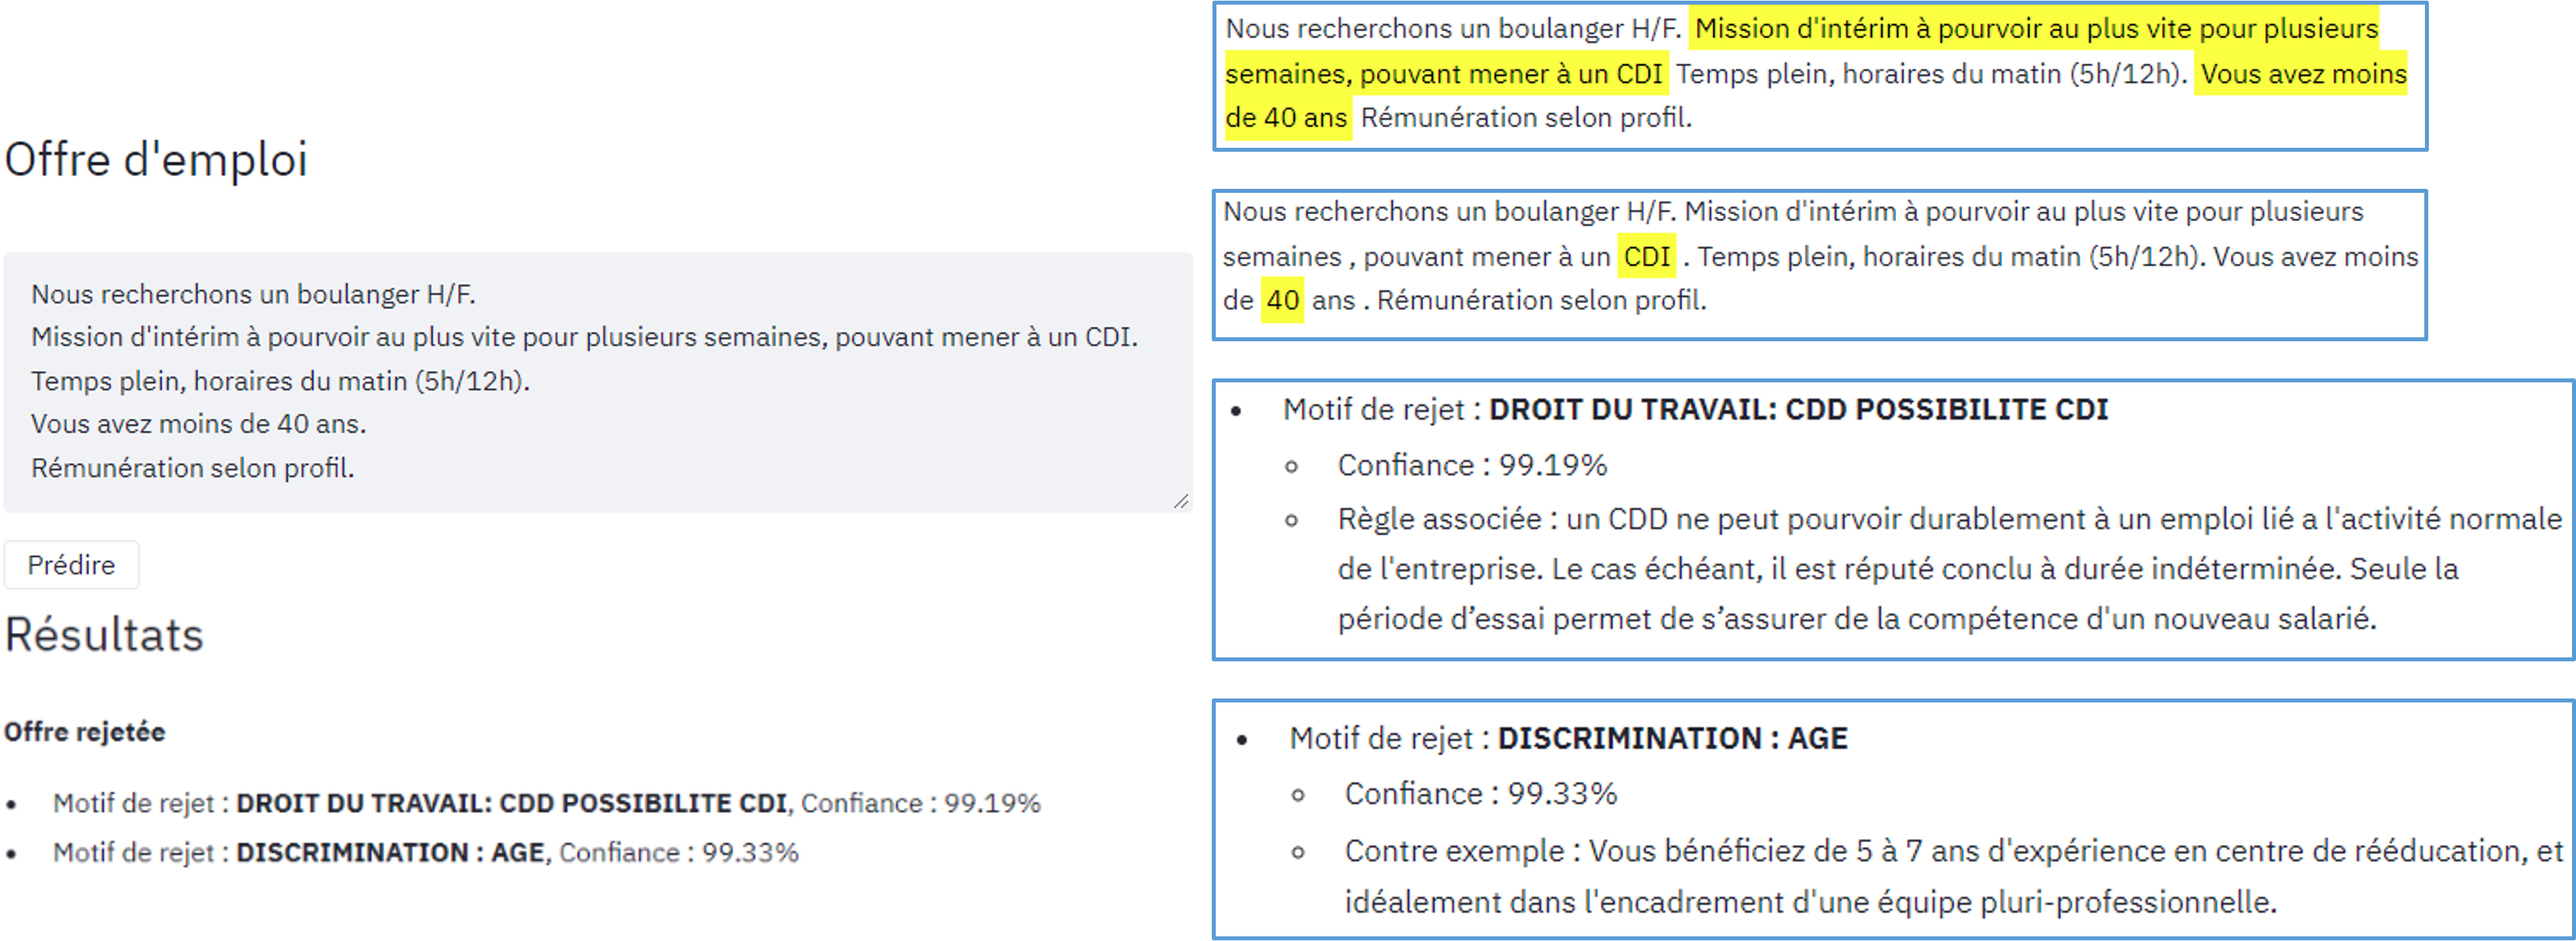
\includegraphics[width=\textwidth]{./S2-Explicabilite_locale/figures/explications_locales.png}
    \caption{Montage présentant un condensé des différentes interfaces développées.}
    \label{fig:explications_locales}
\end{figure}

\paragraph{Explication par phrase} Cette explication consiste à surligner l'ensemble des phrases rejetées par le système, comme illustré dans la figure~\ref{fig:demo_phrase}.
% comment
\begin{itemize}
    \item Si le modèle d'IA renvoie un motif de rejet pour une phrase, alors le texte est réaffiché dans l'encart ``Résultats'', et la phrase en question est surlignée.
    \item Si plusieurs phrases sont surlignées, le texte n'apparaît qu'une fois et contient toutes les phrases surlignées.
    \item Les motifs de rejets sont affichés dans l'ordre d'apparition dans l'offre.
\end{itemize}
Ainsi, dans la figure~\ref{fig:demo_phrase}, la phrase ``Mission d'intérim à pourvoir [...] pouvant mener à un CDI.'' est associée au premier motif de rejet \textit{Droit du travail : CDD possibilité CDI}.

\begin{figure}[htpb!]
 \centering
 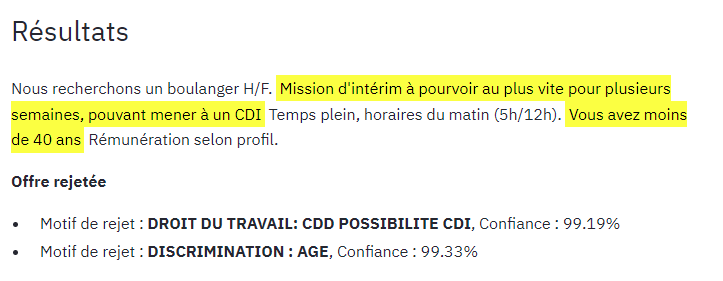
\includegraphics[width=0.7\textwidth]{S2-Explicabilite_locale/figures/demo_phrase.png}
 \caption{Démonstrateur présentant l'interface pour l'explication par phrase(s) surlignée(s).}
 \label{fig:demo_phrase}
\end{figure}

% Avantage
Ce type d'explication a l'avantage d'être peu couteux à mettre en place. Il est rapide, car ne nécessite pas de calcul supplémentaire après inférence. Il met en avant le contexte du rejet, laissant le soin à l'utilisateur d'analyser la ou les phrases en rejet.
% inconvénient
Toutefois, en surlignant toute la phase, la visualisation est peu précise. C'est un problème si une phrase est longue, ou si un texte est mal formaté et ne comporte pas de ponctuation permettant de séparer les phrases. De même, le comportement interne du modèle n'est pas explicité.

\paragraph{Explication mot à mot} Sur le même principe que l'explication par phrase, l'explication par mot surligne le ou les mots menant à la décision de rejet par le système. Comme illustré dans les figures~\ref{fig:demo_mot}, pour chaque phrase rejetée par le système, les mots sont surlignés dans le texte. Les motifs de rejets sont toujours affichés dans l'ordre d'apparition. Les mots à surligner sont déterminés par une méthode d'explication basée sur les importances de variables, ici avec la méthode d'attention. Plus de détails sur la sélection de ces mots sont donnés en section~\ref{C2:explications}. Sur la figure~\ref{fig:demo_mot_1}, le motif de rejet \textit{Droit du travail : CDD possibilité CDI} est ainsi lié à la présence du mot ``CDI'' dans le texte. À noter que la seule présence du mot n'est pas une explication suffisante, le contexte étant également pris en compte. Par exemple dans la figure~\ref{fig:demo_mot_2}, la seconde phrase n'est plus rejetée mais comporte toujours le mot ``CDI''.

\begin{figure}[htpb!]
    \centering
    \begin{subfigure}[b]{0.48\textwidth}
        \centering 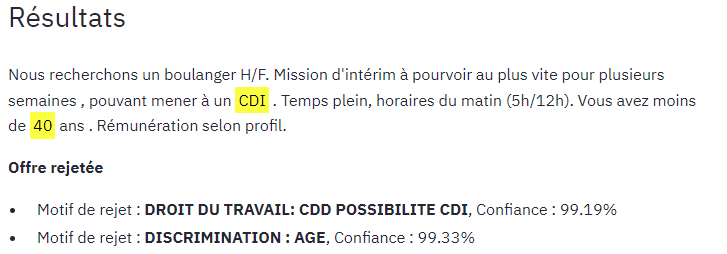
\includegraphics[width=\textwidth]{S2-Explicabilite_locale/figures/demo_mot.png}
        \caption{Explication pour deux phrases en rejet}
        \label{fig:demo_mot_1}
    \end{subfigure}
    ~
    \begin{subfigure}[b]{0.48\textwidth}
        \centering 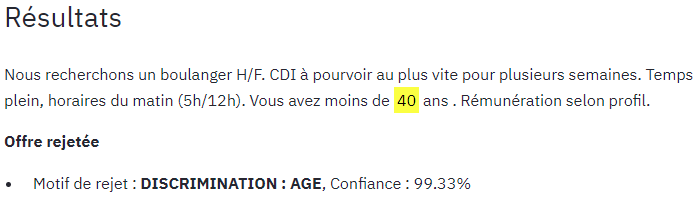
\includegraphics[width=\textwidth]{S2-Explicabilite_locale/figures/demo_mot_2.png}
        \caption{Explication pour une seule phrase rejetée}
        \label{fig:demo_mot_2}
    \end{subfigure}
    ~
    \caption{Démonstrateur présentant l'explication mot à mot
 }\label{fig:demo_mot}
\end{figure}

% Avantage
L'explication mot à mot est précise, et reflète le comportement du modèle d'IA étudié, plus ou moins fidèlement selon la méthode d'explication employée.
% inconvénient
Néanmoins, ce type d'explication nécessite un calcul supplémentaire, afin de déterminer les mots responsables du rejet. Il complexifie l'outil, et ajoute un délai pour afficher l'explication.

\paragraph{Règle} Afficher une règle métier constitue une explication courte, extraite des documents de référence et associée au motif de rejet détecté. Cette interface réalisée à la demande des utilisateurs est présentée en figure~\ref{fig:demo_regle}.
% comment
Lors de la détection d'une phrase rejetée, le motif de rejet est affiché dans l'encart de résultats. Une règle associée est affichée juste en dessous. La figure~\ref{fig:demo_regle} montre l'affichage de deux motifs de rejets et les règles associées. Une règle est toujours la même pour un motif donné. Elle est définie manuellement pour chacun des 27 motifs de rejet, en résumant brièvement les informations présentes dans le GARO.

\begin{figure}[htpb!]
 \centering
 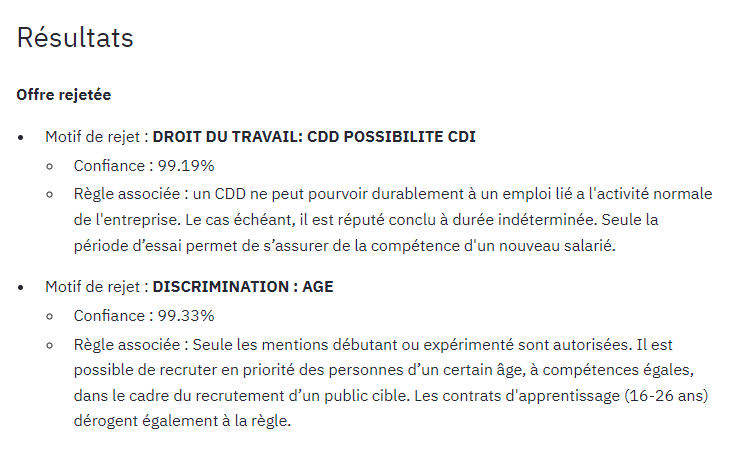
\includegraphics[width=0.7\textwidth]{S2-Explicabilite_locale/figures/demo_regle.png}
 \caption{Démonstrateur pour l'interface d'explication par la règle métier.}
 \label{fig:demo_regle}
\end{figure}

% Avantage
Cette interface a l'avantage d'être facile à mettre en place d'un point de vue technique. Son affichage est rapide, car elle ne nécessite pas de calcul. Elle est plus généralisable qu'un exemple. Elle est basée sur l'expertise métier et les documents de référence, ce qui la rend particulièrement adapté aux utilisateurs non experts, en leur fournissant un premier niveau d'information.
% inconvénient
En contrepartie, cette interface fournit des explications peu précises, parfois insuffisantes dans le cadre de cas délicats. Dans sa version implémentée, elle nécessite un travail manuel afin de résumer le document de référence.

\paragraph{Contre-exemple} On peut également associer une phrase rejetée à une phrase proche de celle-ci, mais acceptée par le système. La figure~\ref{fig:demo_cfe} présente cette interface.
% comment
La création des contre-exemples est une preuve de concept. C'est une version développée dans un temps court, peu efficiente, mais qui donne des pistes de réflexion. Les contre-exemples sont récupérés dans une base restreinte de $100$ phrases légales, appelés ci-après \textit{candidats}. La phrase illégale ainsi que tous les candidats sont rapprochés en les vectorisant via un plongement de mots, puis en rapprochant ces vecteurs avec une distance sémantique : la distance cosinus entre les vecteurs représentant les phrases. Le contre-exemple est la phrase légale ayant la distance cosinus minimale avec la phrase rejetée.  % TODO vérifier

\begin{figure}[htpb!]
\centering
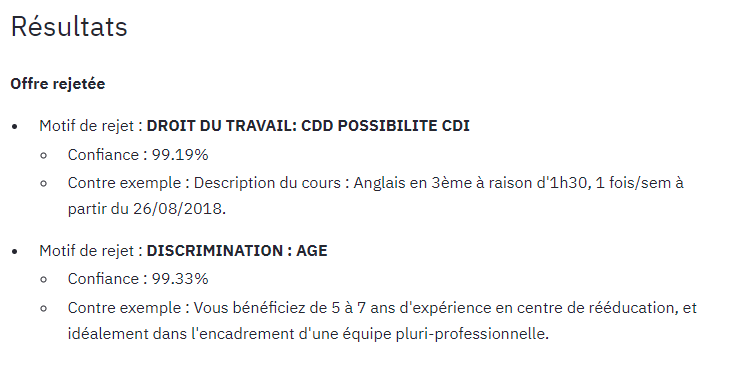
\includegraphics[width=0.7\textwidth]{S2-Explicabilite_locale/figures/demo_cfe.png}
\caption{Démonstrateur pour l'interface d'explication par le contre-exemple.}
\label{fig:demo_cfe}
\end{figure}

% Avantage
Ce type d'explication a l'avantage d'être contrastif, une explication bien perçue par les humains.  %cite.. Miller ?
Le contre-exemple est extrait d'un ensemble de phrases réelles, ce qui réduit le risque d'explications hors distributions, ressemblant à un élément réaliste, mais trompant le modèle d'intelligence artificielle.
Enfin, dans ce cas d'usage, fournir un contre-exemple revient à proposer une correction automatique de l'offre, pour peu que la phrase de contre-exemple soit assez proche de celle d'origine.
% inconvénient
L'inconvénient de cette approche est qu'elle nécessite de bons candidats au contre-exemple. Il est nécessaire de trouver un moyen de filtrer ces bons candidats, car la comparaison par paires de phrase est couteuse en calculs. De même, l'explication avec des candidats qui sont peu intéressants car trop spécifique, ou trop éloignés du sens sémantique d'origine, sont peu intéressants pour les utilisateurs et pourraient générer plus de frustration qu'en enlever.

\subsection{Préférences des utilisateurs} \label{C2:collect_pref}

% Quoi
Nous utilisons l'interface d'explications par surlignage des mots précédemment présentée afin de recueillir les préférences des experts et expertes du domaine. Plusieurs méthodes de collecte sont possibles :
\begin{itemize}
    \item La notation les explications, par exemple sur 5 points. Cela permet de donner une valeur absolue aux méthodes évaluées, mais implique la création d'un barème mental propre à chaque utilisateur.
    \item Le tri des explications. L'utilisateur a ainsi une vision d'ensemble des explications. Cette méthode permet d'ordonner des explications courtes.
    \item La comparaison par paire d'explications. Cette méthode est préférable pour ordonner des explications longues.
\end{itemize}

Nous nous intéressons ici uniquement à l'ordre de préférence et n'avons donc pas besoin de cette valeur absolue. Nous présentons des phrases pouvant être longues, nous privilégions la comparaison par paires d'explication.
C'est un outil efficace car il est plus facile pour un humain de dire quelle explication iel préfère, plutôt que donner une note.

\paragraph{Interface présentée}
Pour recueillir leurs préférences, les utilisateurs se voient présenter deux fois la même phrase dans l'interface d'explication par surlignage des mots importants. La classification du modèle d'IA et une explication par la règle sont également présentées. Ces éléments sont visibles sur la Figure~\ref{fig:expe_ui} dans les deux zones sur fond blanc.

Les utilisateurs sont invités à choisir l'explication répondant à la question : ``Quelle est l'explication la plus utile pour comprendre l'alerte ?'', l'alerte étant la raison du rejet donné par le modèle. Comme le montre la Figure~\ref{fig:expe_ui}, la question est affichée en haut de l'écran pendant toute l'expérience.
La réponse peut être une erreur du modèle. Dans ce cas, les explications fournies peuvent sembler hors sujet aux utilisateurs, comme discuté dans la section~\ref{C2:ground_truth}.
L'explication peut être vide, ce qui signifie qu'il n'y a pas de mot mis en évidence. Si les utilisateurs ne perçoivent aucune préférence entre deux explications, on leur demande d'en choisir une selon leur sentiment subjectif. Comme plusieurs utilisateurs évaluent les mêmes phrases, ces cas apparaîtront dans les données comme des choix difficiles, où aucune explication ne ressort.

\begin{figure}[h!tpb]
  \setlength{\belowcaptionskip}{-20pt}
  \begin{center}
    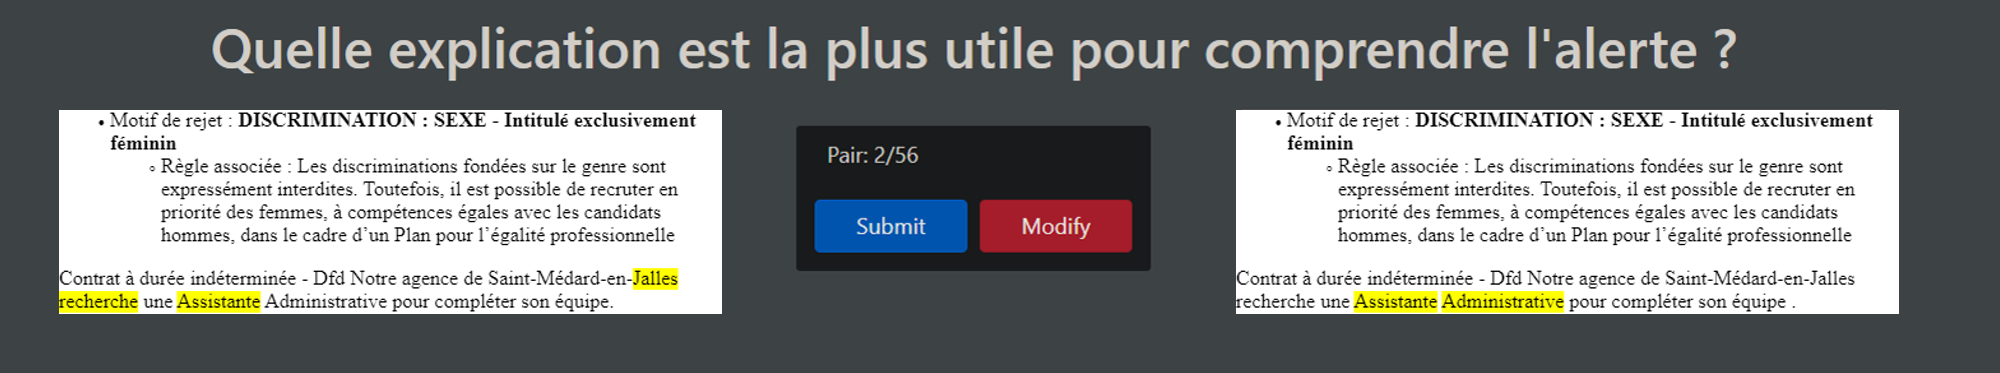
\includegraphics[width=\textwidth]{S3-Comparaison_de_methodes/figures/user_experiment_interface.png}
    \caption{L'interface de l'expérience. Les utilisateurs doivent choisir entre deux explications présentées celle qu'iels préfèrent. La raison du rejet et la règle associée sont affichées. Les explications sont des mots surlignés.}\label{fig:expe_ui}
  \end{center}
\end{figure}

% le profil des utilisateurs
\paragraph{Contraintes expérimentales}
Pour lutter contre le biais d'apprentissage, 14 utilisateurs ont été recrutés par le biais du réseau interne de \textit{P\^ole Emploi}. Ce sont des employés spécialisés dans l’accompagnement des recruteurs, iels possèdent donc une expertise du domaine. Iels sont particulièrement habitués à rédiger et à éditer des offres d'emploi et travaillent depuis de nombreuses années avec une ancienne version de notre solution d'IA basée sur des expressions régulières (regex) qui lèvent des alertes légales. Par conséquent, les utilisateurs de cette expérience sont déjà conscients des cas possibles menant à des faux positifs et négatifs pour le rejet automatique d'offres d'emploi. En définitive, ces experts ne sont pas sujets à des erreurs dues à la découverte du cas d'usage.

% Les précautions
Nous avons également pris en compte la concentration, la fatigue et la faible disponibilité des utilisateurs. Les précautions suivantes ont été prises.
\begin{itemize}
    \item La collecte est divisée en 9 sessions courtes, de 30 minutes chacune.
    \item Les sources de notification telles que les téléphones portables ou les logiciels de communicationsont mises en sourdine.
    \item Chaque utilisateur voit les paires dans un ordre différent.
    \item La tâche donnée est simple, l'interface possède très peu d'éléments, comme le montre la Figure~\ref{fig:expe_ui}.
    \item La tâche de comparaison est conçue pour être réalisée de manière autonome.
    \item L'expérience ne nécessite pas de conditions spécifiques telles que le niveau de lumière ou la colorimétrie de l'écran.
    \item En cas de blocage, les utilisateurs peuvent poser des questions par téléphone ou via leur outil habituel de messagerie instantanée.
\end{itemize}

% Résultat
Cette expérimentation a permis de recueillir les préférences de 14 utilisateurs sur 109 phrases. Tous n'ont pas eu la possibilité d'effectuer la totalité des 9 sessions.
104 sessions ont été réalisé sur les 126, soit $83\%$ des comparaisons à effectuer.
9 participants ont réalisé la totalité des sessions. Eut égard de la difficulté de mobiliser les experts et expertes, il était prévu que toutes les comparaisons ne soient pas effectuées.

% conclusion section
% rappel objectif
Nous avons présenté le test d'utilisabilité, de son déroulement en section~\ref{C3:discussion} aux conclusions tirées des entretiens en section~\ref{C3:solution}. Les retours des utilisateurs nous ont aidés à définir des interfaces mieux adaptées à leur besoins. La figure~\ref{fig:explications_locales} montre les interfaces finales conçues dans le démonstrateur présenté dans le chapitre précédent.
La section suivante présente l'évaluation de méthodes d'explications sans utilisateurs.

\section{\'Evaluation sans utilisateurs} \label{C3:iou_expe}

% Quoi
L'évaluation présentée fournit de premiers résultats, lorsqu'il n'y a pas d'utilisateur expert du domaine disponible. Nous cherchons à savoir quelle méthode d'explication convient le mieux à chaque cas d'usage dans son contexte donné.
Ces expérimentations sans utilisateurs permettent de valider des propriétés telles que la concision ou la représentativité, ainsi que décrites en introduction.

% Comment
Nous divisons notre problème en deux questions.
\begin{enumerate}
    \item Cette explication est-elle proche d'une explication idéale ? Nous répondons à cette question de façon quantitative, en mesurant la proximité entre explications générées et de référence.
    \item Lorsqu'il n'y a pas de référence, comment évaluer les méthodes d'explication ? Nous optons pour une approche qualitative, en filtrant pour analyser uniquement les cas où les explications générées sont peu similaires.
\end{enumerate}
Les réponses à ces deux questions permettent d'établir une première évaluation des méthodes appliquées.
Nous appliquons ce protocole aux explications générées dans le chapitre précédent.
Nous nous assurerons notamment que les explications sont concises, fidèles et adaptées aux receveurs
% plan
Nous présentons dans la section~\ref{C3:qt_metric} l'étude quantitative des explications, puis en section~\ref{C3:ql} l'analyse qualitative.

\subsection{Spécificités du cas d'usage Yelp} \label{C3:cu_yelp}

Le cas d'usage Yelp est utilisé afin de généraliser notre protocole. Il est basé sur l'application du même nom permettant à des utilisateurs de noter et donner des avis sur des commerces dont iels ont été clients. La tâche est de retrouver le nombre d'étoiles, entre 1 et 5, associées à un avis utilisateur. Si ce n'est la langue qui est l'anglais, Yelp est, comme le cas d'usage LEGO, un problème de classification de texte, multi-label, multi-classe. L'ensemble d'entraînement contient $453 600$ avis.

% Comment
Ce cas d'usage requiert une version spécifique du réseau d'attention. Les textes sont vectorisés avec un plongement de mots spécifique à l'anglais, générant des vecteurs de 100 dimensions, et basé sur Wikipédia dans sa version anglophone\footnote{\url{https://wikipedia2vec.github.io/wikipedia2vec/pretrained/}}. L'optimiseur est Adam, avec un taux d'apprentissage de $0,0005$.
Ce réseau obtient une précision de $74,63\%$ sur son ensemble de test. En comparaison, les auteurs de~\cite{Lin2017} présentent dans leur article une précision de $64.21\%$ sur leur propre jeu de test.

% comparaison des modèles pour générer les explications avec YELP et LEGO
L'architecture précise du modèle à attention est présentée en C2, pour le cas d'usage LEGO. Ici, nous présentons les différences entre les deux architectures.
\begin{table}
\caption{Comparaison des architectures des réseaux de neurones pour YELP par rapport à LEGO.}\label{model_architecture}
\begin{tabular}{|l|p{0.23\textwidth}|p{0.1\textwidth}|p{0.1\textwidth}|p{0.42\textwidth}|}
\hline
\textbf{ID} & \textbf{Type de couche} & \textbf{YELP} & \textbf{LEGO} & \textbf{Commentaires} \\ \hline
1 & Couche d'entrée    & 300  & 80  & La taille est le nombre de mots dans les textes \\ \hline
2 & Plongement de mots & 100  & 300 & Plongement de mots Word2vec\\ \hline
3 & Bi-LSTM            & $u=$150  & $u=$50  & La sortie est la matrice d'états cachés H \\ \hline
4 & Couche dense 0     & $d_a=$350  & $d_a=$300 & Activation $tanh$ \\ \hline
5 & Couche dense 1     & $r=$1    & $r=$1   &  La sortie est la matrice d'attention A \\ \hline
6 & Représentation     & sortie: $[2u,r]$ & sortie: $[2u,r]$   & Combinaison de l'attention et de la couche cachée, $M=A^T*H$  \\ \hline
7 & Couche dense 2     & 1000 &  $\emptyset$   & Activation $ReLu$ , pour Yelp uniquement \\ \hline
8 & Couche dense 3     & 5    & 28  & Couche de sortie \\ \hline
\end{tabular}
\end{table}

Deux explications sont extraites de ce modèle : les explications par les ancres et les explications d'attention avec un seuil $t=0,15$. Le tableau~\ref{exemple_yelp} illustre ces explications sur une évaluation du jeu de données Yelp. L'étude utilisateur n'est pas réalisée dans ce cas d'usage, il n'y a donc qu'un seul seuil d'attention généré. Comme l'explication des ancres sur de grands textes entraîne souvent des problèmes de mémoire, les ancres ont été appliquées à un sous-ensemble de 1060 évaluations les plus courtes sur les 2653 évaluations de l'ensemble de test complet.

\begin{table}[h!tpb]
\caption{Exemples extraits de Yelp : deux critiques avec des notes et des explications pour les ancres et les méthodes d'attention. Le texte est au-dessus des autres informations.}\label{exemple_yelp}
\begin{tabular}{|p{0.19\textwidth}|p{0.18\textwidth}|l|}
\cline{1-3}
\textbf{Note} & \textbf{Ancres} & \textbf{Attention 0.15} \\ \hline
\multicolumn{3}{|p{0.95\textwidth}|}{``Wow! Superb Maids did an amazing job cleaning my house. They stayed as long as it took to make sure everything was immaculate. I will be using them on a regular basis.''}\\ \hline
5 & {[}{]} &  ['superb', 'amazing', 'everything'] \\ \cline{1-3}
\multicolumn{3}{|p{0.95\textwidth}|}{``For the record, this place is not gay friendly. Very homophobic and sad for 2019. Avoid at all costs''} \\ \hline
1 & ['not'] & ['record', 'not', 'homophobic', 'sad', 'avoid'] \\ \cline{1-3}
\end{tabular}
\end{table}

Une fois les explications générées pour les deux cas d'usage, il reste un dernier type d'explication à récupérer pour mener à bien la suite des expérimentations : les explications des utilisateurs.

\subsection{Analyse quantitative} \label{C3:qt_metric}

% quoi
Dans un premier temps nous cherchons à répondre à la première question : ``Cette explication est-elle proche d'une explication idéale ?''.
Pour cela, nous comparons les explications générées à l'explication de référence,  considérée comme le meilleur résultat possible.
%pourquoi
Ces mesures ont pour objectif de savoir quelles sont les explications les plus fidèles, adaptées au receveur et concises.

%comment
La concision des explications est mesurée par le nombre de mots des explications.
Pour quantifier l'adaptation au receveur et la fidélité, les explications générées sont comparées à la référence (voir section~\ref{C2:ground_truth}). Une métrique simple de similarité entre deux ensembles a été reprise, l'IOU, et est utilisée parmi d'autres métriques connues (précision, score F1...).
Tel qu'utilisé dans~\cite{Bau2017}, l'IOU, l'exactitude et le score F1 sont également comparés, ainsi que le rappel et la précision utilisés dans le score F1. Le rappel est une mesure intéressante car elle n'est pas affectée par les vrais négatifs

% résultats
La concision est peu différenciante pour Yelp, les longueurs moyennes des explications étant similaires, 2,34 et 2,13 mots pour les ancres et l'attention respectivement.
Pour LEGO, les explications basées sur les ancres sont en moyenne plus courtes que celles basées sur l'attention. Les longueurs moyennes sont respectivement de 0,15 et 0,33 mots dans l'ensemble de test. La valeur moyenne est faible en raison des explications vides.
Ces mesures comparent la référence aux explications générées pour le jeu de données LEGO - Bonnes Prédictions (BP). Pour obtenir des mesures équitables, les mots vides ne sont pas pris en compte. L'évaluation du modèle n'étant pas le but de cette expérimentation, le jeu de test utilisé est le jeu de données LEGO - BP de 147 phrases correctement prédites.

\begin{table}[h!tpb]
  \centering
%  \addtolength{\parskip}{-0.5mm}
\caption{Comparaison des explications générées avec la référence, jeu de données LEGO BP. Les meilleurs résultats sont en gras. L'attention obtient des résultats légèrement meilleurs.}\label{anchors_gt_lego_success}
\begin{tabular}{|l|l|c|c|}
  \hline
  \textbf{Mesure} & \textbf{Ancres} & \textbf{Attention} \\ \hline
  % IOU           & 0.938 & 0.930 \\ \hline
  % Acc           & 0.980 & 0.973 \\ \hline
  % Recall        & 0.970 & 0.976 \\ \hline
  % Précision     & 0.961 & 0.943 \\ \hline
  % F1            & 0.965 & 0.959 \\ \hline
  IOU             & $0,94$ & $0,93$ \\ \hline
  Taux de reconnaissance & $0,98$ & $0,97$ \\ \hline
  Rappel          & $0,97$ & $0,98$ \\ \hline
  Précision       & $0,96$ & $0,94$ \\ \hline
  F1              & $0,97$ & $0,96$ \\ \hline
\end{tabular}
\end{table}

Les résultats de toutes les métriques pour le cas d'usage LEGO sont affichés dans le tableau~\ref{anchors_gt_lego_success}. Dans l'ensemble, comparées à la référence, les deux méthodes de génération d'explication obtiennent des résultats similaires, cf. Tableau~\ref{anchors_gt_lego_success}.
Les scores sont élevés, en partie à cause du nombre de phrases non rejetées dans le jeu de données LEGO - BP : 131. Ces instances n'ont pas d'explication, les différentes métriques sont dans ce cas égales à 1.

% analyse
Les ancres et l'attention sont également comparées les unes aux autres. En l'absence de référence, les métriques telles que la précision et le score F1 ne sont pas pertinentes. Une IOU élevée indique que les explications sont similaires dans les deux méthodes. L'IOU entre les ancres et l'attention est de $0,92$, ce qui indique qu'elles donnent des résultats similaires. Pour le cas d'usage LEGO, les explications des ancres et de l'attention sont toutes deux similaires et proches de l'explication idéale.

% Petit point sur YELP
Comme il n'y a pas de documentation ni d'expert du domaine pour le cas d'usage Yelp, il n'y a pas de référence pour son jeu de données. Par conséquent, la comparaison n'est possible qu'entre les ancres et les explications d'attention. L'IOU indique si les explications générées sont similaires. La moyenne de l’IOU sur l'ensemble de test réussi est de $0,23$, ce qui montre de fortes différences entre les deux méthodes d'explication. Cela peut s'expliquer par les longs textes et le vaste vocabulaire attendu dans les explications. Par conséquent, pour évaluer les méthodes d'explication dans le cas d'usage de Yelp, une analyse qualitative est nécessaire.

En définitive, l'analyse quantitative donne une première analyse sur chaque cas d'usage. Pour LEGO, les ancres sont plus concises, et aussi fidèles et adaptées que l'attention. Pour Yelp, les deux méthodes sont proches en concision, mais diffèrent beaucoup en contenu. Le manque de données ne permet pas de juger de leur fidélité ni de leur adaptation aux personnes cibles.

\subsection{Analyse qualitative} \label{C3:ql}

% quoi
Cette première analyse nous amène à la deuxième question : ``Lorsqu'il n'y a pas d'explication humaine, comment évaluer les méthodes d'explication ?''
En effet il n'y a pas toujours de données de référence à disposition, c'est le cas pour Yelp. Dans ce cas, l'alternative est l'analyse qualitative par un humain, une tâche longue et coûteuse. Nous proposons une évaluation qualitative de la fidélité et l'adaptation des ancres et de l'attention de manière efficiente, en effectuant un filtre sur les exemples d'intérêt.

Ces éléments pertinents sont ceux pour lesquels les explications à comparer sont très différentes.
% permet de donner un premier regard qualitatif sur les explications générées
Cela permettra de déterminer si une méthode d'explication est plus précise lorsqu'elle est différente.
Dans le contexte d'une expérience sans experts du domaine, cela permet à un expert en données de procéder à la première évaluation des différentes méthodes d'explication.

%comment
Ce filtrage sera donc utilisé dans l'analyse qualitative suivante pour les deux cas d'usage. Les phrases d'intérêt sont celles avec une forte différence entre explications générées par les différentes méthodes. Le filtrage de ces phrases se fait donc sur l'IOU entre méthodes, en conservant les phrases pour lesquelles l'IOU est la plus faible.

% résultats
\begin{table}[htb!p]
\caption{Textes de LEGO avec différentes explications (IOU inférieure à $0,5$). Le texte est au-dessus des autres informations.}\label{qualitative_lego}
\begin{tabular}{|l|p{0.21\textwidth}|p{0.27\textwidth}|p{0.25\textwidth}|}
    \cline{1-4}
    \textbf{Motif de rejet} & \textbf{Vérité terrain} & \textbf{Ancre} & \textbf{Attention 0.15}  \\ \hline
    \multicolumn{4}{|p{0.96\textwidth}|}{``Contrat a duree indeterminee - Dfd Notre agence de Saint-Medard-en-Jalles recherche une Assistante Administrative pour completer son equipe.''}\\ \hline
    Genre & ['assistante, administrative'] & ['recherche', 'Assistante', 'Jalles'] & ['assistante', 'administrative'] \\ \cline{1-4}
    \multicolumn{4}{|p{0.96\textwidth}|}{``Nous recherchons actuellement un Teleconseiller FRANCAIS / NEERLANDAIS (H/F) pour le compte de notre client, a Marcq-en-Baroeul.''}  \\ \hline
    Nationalité & ['francais, neerlandais'] &['un', 'neerlandais', 'recherchons', 'francais'] & ['neerlandais'] \\ \cline{1-4}
\end{tabular}
\end{table}

Pour le cas d'usage LEGO, le tableau~\ref{qualitative_lego} donne des exemples où la valeur de l'IOU est inférieure à 0,5. Cette analyse qualitative indique que les explications d'attention sont une meilleure méthode d'explication pour ce cas d'usage.

\begin{table}[htb!p]
\caption{Textes de YELP avec explications. Le texte est au-dessus des autres informations.}\label{qualitative_yelp}
\begin{tabular}{|p{0.1\textwidth}|p{0.2\textwidth}|l|}
\cline{1-3}
\textbf{\'Etoiles} & \textbf{Ancres} & \textbf{Attention 0.15} \\ \hline
\multicolumn{3}{|p{0.96\textwidth}|}{Wow!  Superb Maids did an amazing job cleaning my house.  They stayed as long as it took to make sure everything was immaculate.  I will be using them on a regular basis.}\\ \hline
5 & {[}{]}  &   ['superb', 'amazing', 'everything'] \\ \cline{1-3}
\multicolumn{3}{|p{0.96\textwidth}|}{For the record, this place is not gay friendly. Very homophobic and sad for 2019. Avoid at all costs}  \\ \hline
1 & ['not'] & ['record', 'not', 'homophobic', 'sad', 'avoid'] \\ \cline{1-3}
\multicolumn{3}{|p{0.96\textwidth}|}{Had the best experience buying my dress at brilliant bridal in jan 2018. Can't wait to wear my beautiful gown in oct 2018}  \\ \cline{1-3}
5 & ['brilliant']  &  ['best', 'buying', 'can']  \\ \cline{1-3}
\end{tabular}
\end{table}

% Analyse
Le tableau~\ref{qualitative_yelp} illustre des exemples d'évaluations Yelp et les explications associées pour les évaluations extrêmes (5 et 1 étoiles) lorsque les explications sont différentes. Il indique un manque de mots significatifs dans les ancres. Comme les longueurs moyennes sont similaires et que l'attention semble plus précise lorsque les explications sont très différentes, cette analyse qualitative indique que les explications basées sur l'attention sont un choix plus sûr dans ce cas d'usage particulier.

Pour le cas d'usage Yelp, les deux explications mettent en évidence les mêmes parties lorsque les évaluateurs mentionnent leurs propres évaluations. Cela conduit même à des prédictions erronées, comme le montre le tableau~\ref{stars_yelp}. Puisque le texte mentionne 2 étoiles, l'évaluation prédite est de 2 étoiles. La note réelle était de 3 étoiles, mais les explications font toutes deux ressortir le ``2'' du texte.

\begin{table}[h!tpb]
    \centering
\caption{ Influence de la notation montrée par explication dans le cas d’usage Yelp.}\label{stars_yelp}
\begin{tabular}{|p{0.35\textwidth}|l|p{0.17\textwidth}|p{0.14\textwidth}|p{0.14\textwidth}|}
  \hline
  \textbf{Description} & \textbf{Note} & \textbf{Note prédite} & \textbf{Ancres} & \textbf{Attention 0.15} \\ \hline
  ``[...] And this is the reason I gave them a mere 2 stars[...]'' & 3 & 2 & ['2', 'stars'] & ['2'] \\ \hline
\end{tabular}
\end{table}

% conclusion, transition
L'évaluation sans explication de référence tend à la même conclusion pour les deux cas d'usage. L'IOU permet de sélectionner des phrases intéressantes à analyser, diminuant l'effort d'analyse. L'explication par l'attention s'est avérée être la méthode la plus fidèle.

En résumé, l'expérience sans experts du domaine donne des indications sur différentes propriétés. Premièrement, les explications par les ancres sont plus concises pour LEGO, mais de taille similaire aux explications par attention pour Yelp. Enfin, les explications par attention sont plus fidèles pour Yelp, et légèrement plus fidèles et adaptées aux receveurs pour LEGO. Selon la propriété, fidélité ou concision, à privilégier pour LEGO, l'une ou l'autre méthode sera à choisir. Pour Yelp, l'analyse qualitative met en avant les explications à attention.

Cette première expérience a été conçue pour donner une première évaluation de plusieurs méthodes d'explication lorsque les utilisateurs et utilisatrices experts sont hors de portée. La section suivante présente une expérience plus importante, avec des utilisateurs impliqués.

\section{\'Etude psychométrique avec experts du domaine} \label{C3:pus}

% Quoi
Cette étude vise à évaluer les méthodes d'explication lorsque des utilisateurs et utilisatrices experts du domaine sont disponibles.
Cette étude est illustrée avec le cas d'usage LEGO. Yelp ne sera pas traité dans cette partie car nous ne disposons pas de sujets experts pour appliquer le protocole décrit.

% Pourquoi
Cette analyse répond à deux questions : ``Quelle explication est préférée par les experts du domaine ?'' et ``Comment faire en sorte que la métrique quantitative corresponde aux préférences des utilisateurs ?''.
% Comment
Comme le but est de travailler avec les préférences, le jeu de données de test est différent de celui de la section~\ref{C3:iou_expe}. Le jeu de données LEGO - DE de 106 phrases sera utilisé. Ce filtre évite que les utilisateurs se retrouvent avec des explications identiques à comparer.
Les préférences humaines sont comparées aux performances mesurées par similarité entre explications générées et explications de référence.

% objectif & résultats
La section fournit une vue d'ensemble du protocole d'étude psychométrique, ainsi que nombre de détails permettant son implémentation adaptée.
Les résultats obtenus par l'application de ce protocole ne donnent pas de méthode vainqueure claire au global. Une analyse approfondie des résultats montre que les méthodes préférées évoluent selon la complexité des explications de référence. La notion de concision est ainsi à prendre en compte dans l'évaluation des performances.

% plan
Le protocole expérimental est détaillé en section~\ref{C3:protocole_expe}.
Les calculs nécessaires pour classer les méthodes par performance et préférence sont respectivement présentés en sections~\ref{C3:iou_lego_de} et~\ref{C3:pref_humaine}. Enfin, les résultats sont présentés et analysés en section~\ref{C3:pus_result}.

\subsection{Protocole expérimental} \label{C3:protocole_expe}

% Quoi
Cette section présente le protocole de ce deuxième volet d'évaluation de méthodes d'explication.
% Pourquoi
Ce processus permet d'évaluer les méthodes d'explication qui prennent en compte les préférences des utilisateurs. L'objectif est double. Premièrement, recueillir les préférences humaines pour les méthodes d'explication. Deuxièmement, valider une métrique quantitative pour estimer les préférences des utilisateurs.
% Comment
En utilisant la figure~\ref{fig:experiment} comme support, le processus complet est  décrit en suivant les flèches du diagramme.

\begin{figure}[h!tpb]
  \setlength{\belowcaptionskip}{-20pt}
 \begin{center}
  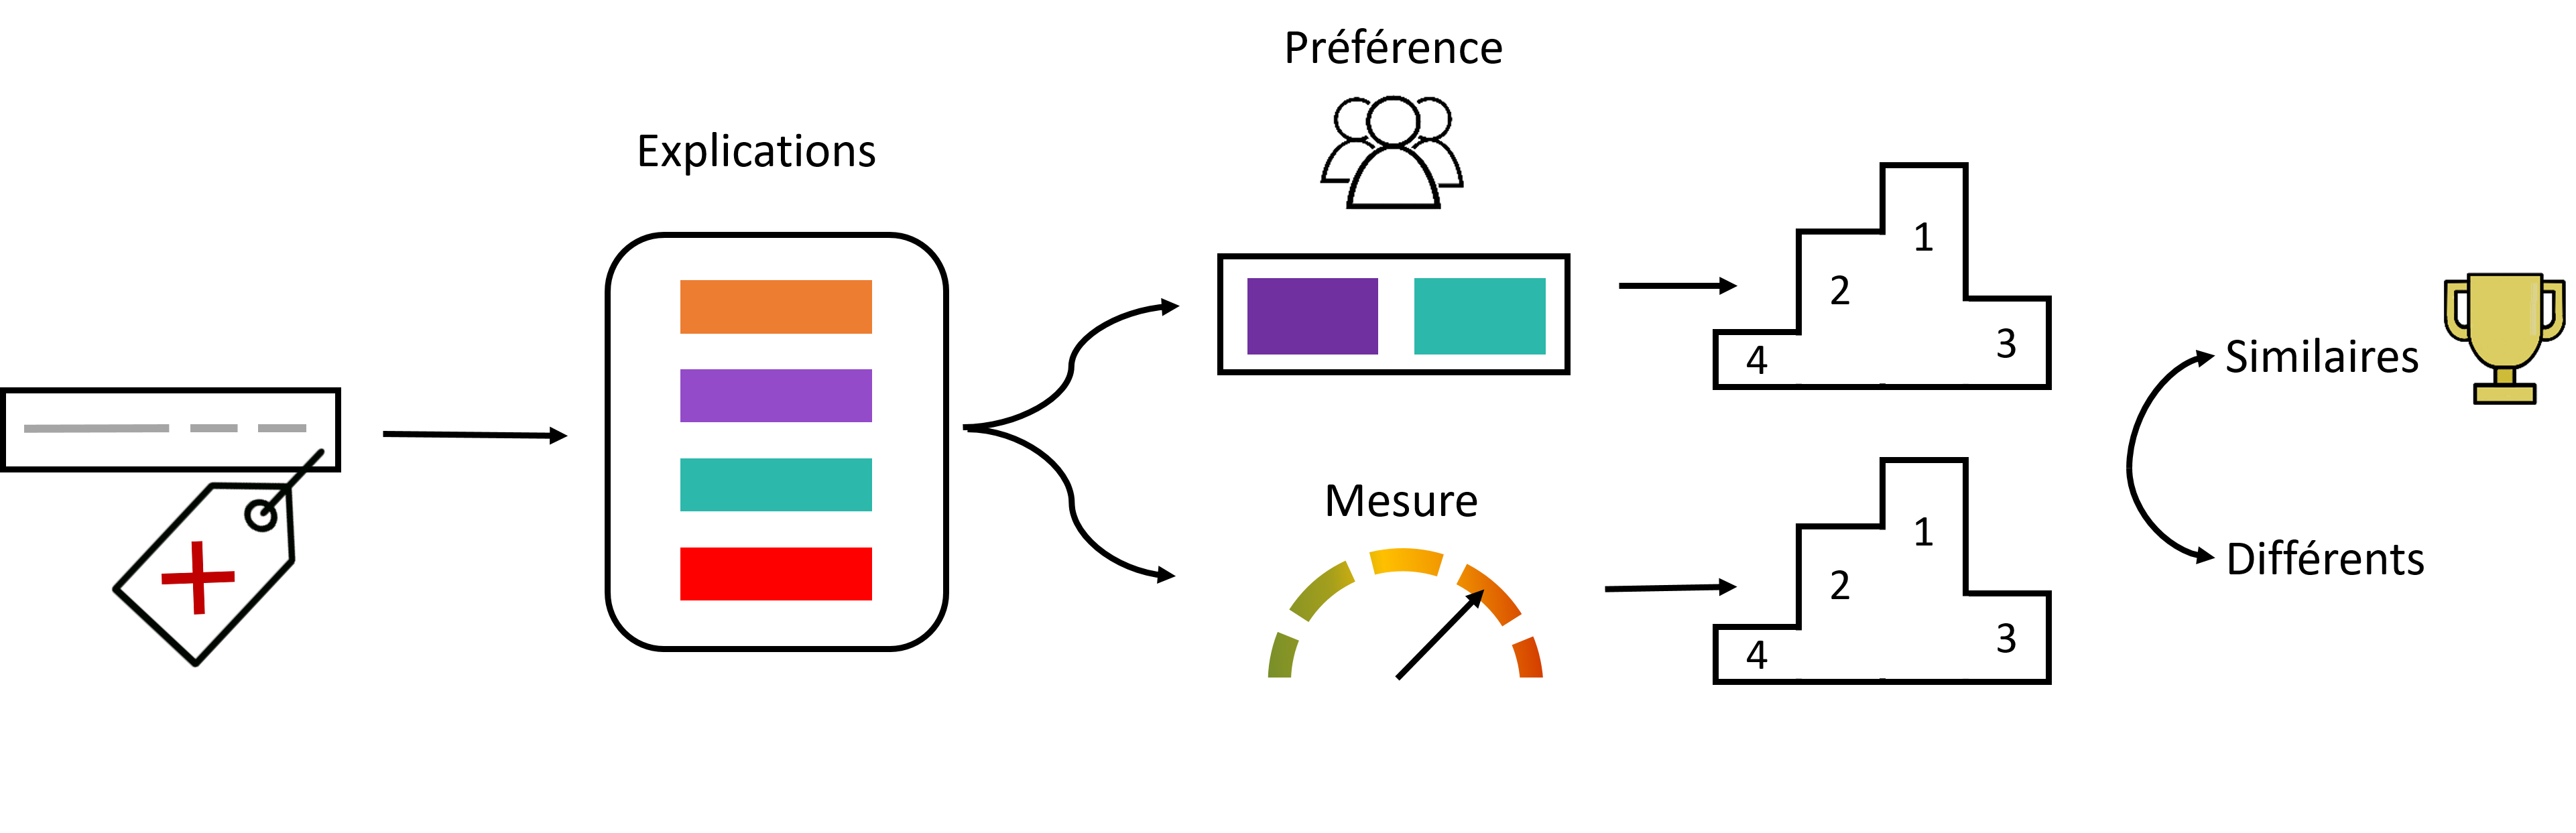
\includegraphics[width=\textwidth]{S3-Comparaison_de_methodes/figures/experiment.png} %
  \caption{Processus global de l'expérience, avec étude psychométrique des utilisateurs et analyse quantitative.}\label{fig:experiment}
 \end{center}
\end{figure}

Tout d'abord, des données étiquetées sont fournies au modèle et aux méthodes d'explication à évaluer. Comme la comparaison par paires est réalisée plus tard, nous recommandons de ne considérer que quelques méthodes d'explication évaluées à la fois.

Pour obtenir la métrique quantitative, les explications générées sont comparées à la référence.
La première version est une métrique simple, ici l'IOU comme vu dans la section~\ref{C3:qt_metric}. Encore une fois, la référence est considérée comme la meilleure option par conception et obtient le score maximal de 1. Les autres explications obtiennent des scores compris entre 0 et 1, 1 étant le meilleur. En classant les méthodes d'explication par leur score moyen, on obtient le classement quantitatif.

La comparaison par paires du chapitre précédent donne une matrice de préférences. L'élément $i,j$ de cette matrice indique le nombre de fois où $i$ a été préféré à $j$. Pour obtenir un classement à partir de cette matrice, l'algorithme Bradley-Terry-Luce (BTL)~\cite{Bradley1952,Luce1959} est utilisé. Il permet de transformer une matrice de comparaison par paires en un classement ordonné de tous les éléments comparés. Nous obtenons ainsi une échelle psychométrique ordonnant les quatre méthodes d'explication : la référence et les explications générées.

Une fois les podiums définis, nous pouvons les comparer. Si le classement de la métrique quantitative est similaire aux préférences humaines, nous pouvons estimer sans risque que la métrique reflète les préférences des utilisateurs. La métrique peut être conservée et réutilisée avec d'autres méthodes d'explication si nécessaire.
Si le classement de la métrique quantitative n'est pas similaire aux préférences des utilisateurs, alors notre métrique quantitative doit être améliorée. Une analyse des données de cette expérience donnera des pistes sur ce qu'il faut améliorer.

Ce protocole est appliqué au cas d'usage LEGO. Toutefois, il doit être adapté pour chaque cas d'usage, avec si besoin un format de données différent, un nombre variable de méthodes d'explication, et une métrique quantitative personnalisée.

% Les données consistent ici en des phrases d'offres d'emploi comme entrées textuelles avec leurs étiquettes associées : raison du rejet.

La génération des explications est décrite dans le chapitre précédent. Comme les ancres doivent être générées avec un modèle, le modèle d'attention est utilisé pour générer l'étiquette. Cela garantit que les différences de modèle n'auront pas d'impact sur l'expérience. Dans ce travail, nous comparons les ancres et deux explications de l'attention avec des seuils de valeurs $t = 0,15$ et $t = 0,5$. La deuxième explication avec un seuil $t = 0,5$ est générée spécifiquement pour cette expérimentation. Comme seul le seuil est plus élevé, les explications avec \textit{attention 0,5} sont un sous-ensemble des explications avec \textit{attention 0,15}, avec les mêmes mots ou plus concises. Elles permettent d'étudier le niveau d'information attendu par les utilisateurs. Pour chaque phrase, une explication de référence par attention humaine est également établie, tous les détails sont donnés dans la section~\ref{C2:ground_truth} du chapitre précédent. Une entrée génère quatre éléments à comparer.
% conclusion et prochaine section
Maintenant que l'expérience globale a été présentée, nous procédons à la mesure quantitative de qualité des explications.

\subsection{Mesure quantitative}\label{C3:iou_lego_de}

% Pourquoi
Dans l'expérimentation précédente (cf. section~\ref{C3:iou_expe}) sur le jeu de données LEGO - BP, nous avons considéré la performance des explications en tant que similarité entre explication générées et de référence. Cette similarité est mesurée avec l'IOU. Dans la section courante, nous effectuons cette même mesure, cette fois sur le jeu de données LEGO - DE, puisque la collecte des préférences utilisateurs contraint à ne pas avoir 2 fois la même explication,

La comparaison de la métrique quantitative avec les préférences utilisateurs implique de recalculer l'IOU dans ce jeu de données pour définir le podium de la métrique quantitative.
En raison de cette variation dans la conception du jeu de données, une baisse conséquente de l'IOU est attendue par rapport à l'IOU calculé sur le jeu de données LEGO BP dans la section~\ref{C3:iou_expe} : les phrases conformes du jeu de données LEGO - BP ne sont plus présentes dans le jeu de données LEGO - DE, et tiraient les résultats vers le haut. Le jeu de données LEGO - DE ne contient lui aucune phrase conforme.

% Comment
L'IOU est calculé avec le même protocole qu'en section~\ref{C3:iou_expe}, les mots d'arrêt étant ignorés. Comme le montre la première ligne du tableau~\ref{iou_lego_de_cplx}, les scores baissent de manière significative par rapport aux chiffres présentés dans le tableau~\ref{anchors_gt_lego_success} ce qui était attendu.

Une analyse plus poussée montre que, dans notre cas, cette baisse est principalement due au fait de prendre en compte les cas où le modèle de prédiction est en échec, ces cas étant filtrés dans le jeu de données LEGO - BP. Ainsi, l'IOU entre les ancres et les explications de référence pour le jeu de données DE est en moyenne de $0,27$. Pour les cas où le modèle est en succès elle est en moyenne de $0,52$, pour les cas où il est en échec, l'IOU est de $0,02$.

% Résultats et analyse
\begin{table}[h!tpb]
  \centering
  \addtolength{\parskip}{-0.5mm}
\caption{Comparaison objective des ancres et des explications d'attention. Les explications sont comparées à la référence avec l'IOU, sur le jeu de données LEGO - DE.}\label{iou_lego_de_cplx}
\begin{tabular}{|l|l|c|c|c|}
  \hline
  \textbf{Type d'explication} & \textbf{Ancres} & \textbf{Attention 0,15} & \textbf{Attention 0,5} \\ \hline
  Total  (106)  & 0,27 & 0,23 & 0,23 \\ \hline \hline
  Vide (53) & 0,02 & 0,13 & 0,21 \\ \hline
  Simple (12) & 0,53 & 0,58 & 0,46 \\ \hline
  Complexe (41) & 0,51 & 0,25 & 0,20 \\ \hline
\end{tabular}
\end{table}

La première ligne du tableau~\ref{iou_lego_de_cplx} montre une faible différence entre les méthodes. Une analyse plus poussée dans ce cas d'usage implique de différencier les phrases en fonction de leur explication de référence, cette analyse est présentée dans les lignes suivantes du tableau~\ref{iou_lego_de_cplx}. Les phrases conformes n'ont pas de référence. Ces phrases constituent la catégorie d'explication \textit{vide}. Certaines phrases ont des explications attendues \textit{simples}, composées d'un ou deux mots. Enfin, nous regrouperons les explications attendues de trois mots ou plus dans la catégorie \textit{complexe}. Ce regroupement nous donne les scores moyens de similarité pour la Figure~\ref{fig:iou_plot_cplx}.

\begin{figure}[h!tpb]
  \setlength{\belowcaptionskip}{-20pt}
 \begin{center}
  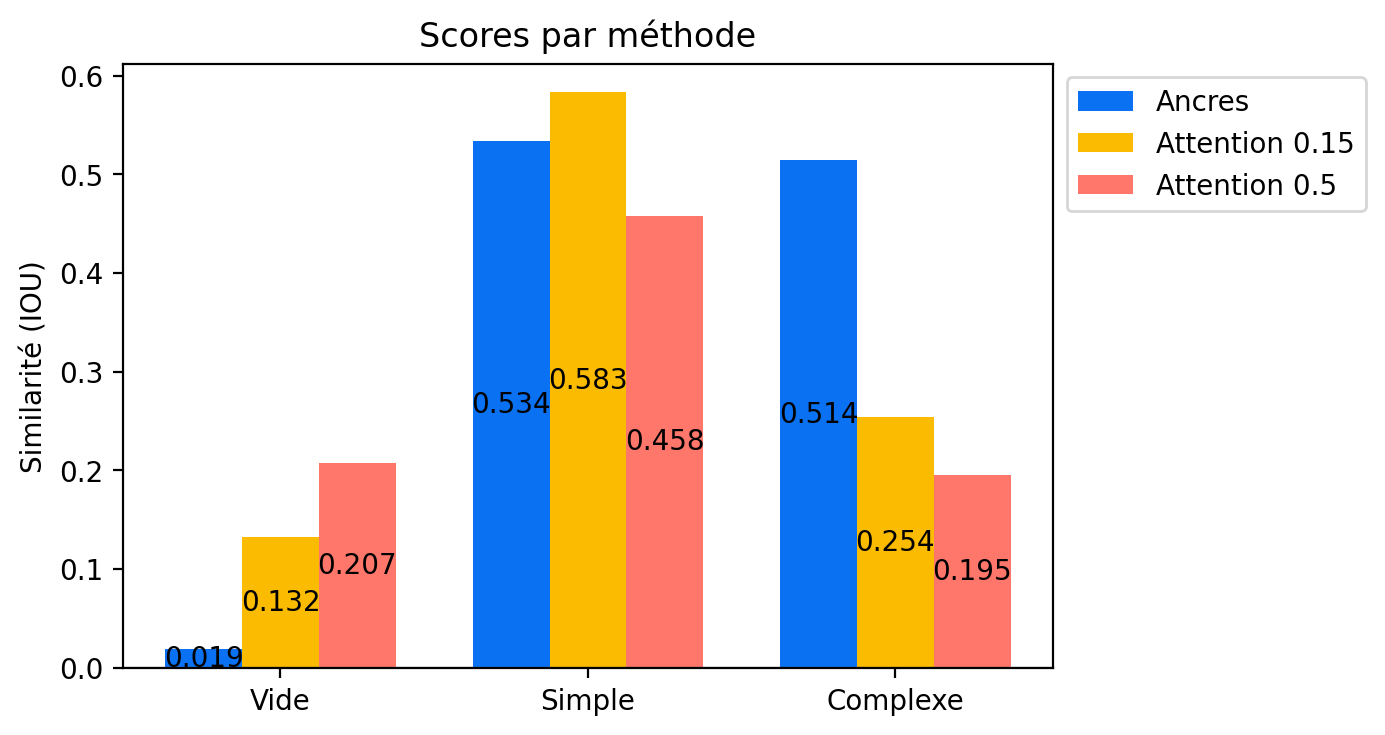
\includegraphics[width=0.9\textwidth]{S3-Comparaison_de_methodes/figures/iou_by_complexity.png}
  \caption{Scores moyens de similarité aux explications de référence, obtenus avec l'IOU pour chaque méthode d'explication, sur le jeu de données LEGO DE.} \label{fig:iou_plot_cplx}
 \end{center}
\end{figure}

Le premier groupe de la figure~\ref{fig:iou_plot_cplx} montre que les trois explications générées ont une faible IOU, en particulier la méthode des ancres. Cela s'explique par le fait que l'IOU avec une explication de référence vide ne peut être que de 0 ou 1. Une IOU de 0 est obtenue lorsqu'une méthode donne n'importe quel mot comme explication, donc l'intersection de cette explication et de l'absence d'explication est de longueur 0. Lorsqu'une méthode ne donne aucune explication, nous comparons deux ensembles vides. Comme ils sont égaux, l'IOU est égale à 1. Comme les méthodes des ancres et d'attention ne donnent rarement aucune explication, leur IOU est très faible par rapport à l'explication humaine, vide.
Le deuxième groupe met en évidence les bonnes performances des méthodes des ancres et d'attention avec $t=0.15$ pour imiter l'explication humaine donnée. Le dernier groupe, pour les cas complexes, indique une divergence significative des deux méthodes d'attention par rapport à l'explication humaine. Cependant, la méthode des ancres conserve une IOU stable entre le 2ème et le 3ème groupe.

\begin{table}[h!tpb]
    \centering
    \addtolength{\parskip}{-0.5mm}
  \caption{Podium basé sur la mesure de similarité, sur le jeu de données LEGO DE, par catégorie d'explication. l'explication humaine sert de référence pour le calcul de l’IOU, elle n'apparaît donc pas dans ce tableau.}\label{qtm_podium}
\begin{tabular}{|l|l|l|l|}
    \hline
        & \textbf{Premier}  & \textbf{Second} & \textbf{Troisième} \\ \hline
Vide     &  Attention 0.5  & Attention 0.15  & Ancre         \\ \hline
Simple   &  Attention 0.15 & Ancre          & Attention 0.5  \\ \hline
Complexe &  Ancre         & Attention 0.15  & Attention 0.5  \\ \hline
\end{tabular}
\end{table}

% conclusion et transition
En définitive, les scores obtenus peuvent être traduits dans le podium du Tableau~\ref{qtm_podium}. Pour rappel, les explications de référence servent au calcul de l'IOU, elles sont considérées comme les meilleures explications pour chaque cas.
Nous avons donc un classement avec l'explication humaine, et les trois autres méthodes dans l'ordre comme indiqué dans le tableau~\ref{qtm_podium}. Ces podiums peuvent maintenant être comparés aux podiums des préférences des utilisateurs. Ces préférences utilisateurs sont abordées dans la section suivante.

\subsection{Préférences des experts} \label{C3:pref_humaine}

% Quoi
Dans cette section, nous classons les types d'explications étudiés selon les préférences des experts du domaine. Nous nous appuyons sur les comparaisons par paires dont la collecte est détaillée dans le chapitre précédent en section~\ref{C2:collect_pref}.
Ces comparaisons permettent le calcul du classement global des méthodes.

% Pourquoi
Ce classement des préférences des experts sera par la suite comparé aux mesures quantitatives. Toutefois en l'état, les comparaisons par paires ne donnent pas de comparaison globale des méthodes d'explications. Nous allons donc dans cette section transformer ces comparaisons par paires en classement global.

% Comment
$A = (a_{ij})_{m \times m}$ est la matrice de préférences issue de la collecte de comparaisons par paires. Chaque coefficient $a_{ij}$ est le nombre de fois où le stimulus (l'explication) $S_i$ a été préféré au stimulus $S_j$. La diagonale de la matrice est nulle.
Le nombre de comparaisons est $n_{ij} = a_{ij}+a_{ji}$ et la probabilité que $S_i$ soit préféré à $S_j$ est $P_{ij} = a_{ij}/n_{ij}$.

Nous obtenons un score de crédit $v_i$ à partir de la matrice de préférences grâce au modèle BTL~\cite{Bradley1952,Luce1959}. Ce modèle se base sur les comparaisons par paires pour estimer les scores $v_i$ selon l'équation~\ref{eq:btl}. Ils sont calculés itérativement pour tous les éléments $i$, puis normalisés en les divisant par la somme des $v_i$, jusqu'à ce que les scores convergent à un état stable.
\begin{equation} \label{eq:btl}
    v_i = \frac{A_i}{\sum_{j \neq i \frac{a_{ij}+a_{ji}}{v_i + v_j}}}
\end{equation}

Ici, le score de crédit $v_i$ représente la probabilité qu'un utilisateur choisisse une méthode plutôt que les autres. Pour un stimulus donné $i$, $A_i$ est la somme des $a_{ij}$ pour tout $j$.
On obtient alors une échelle psychométrique telle que celle de la figure~\ref{fig:btl_plot}. Un score plus élevé indique la préférence des utilisateurs. Comme le score $v_i$ est calculé par rapport aux autres éléments, il n'est pas possible de comparer les scores des éléments $i$ d'une comparaison, avec les éventuels scores $v_k$ obtenus par l'application du BTL à un ensemble différent d'éléments.

% Résultats et analyse
Nous illustrons le calcul des scores avec le cas d'usage LEGO. Les scores BTL peuvent être évalués par phrase. Comme le montre la figure~\ref{fig:btl_plot}, pour cette phrase spécifique, l'échelle psychométrique indique l'ancre comme méthode préférée, et l'explication humaine comme moins appréciée par les utilisateurs.

\begin{figure}[h!tpb]
  \setlength{\belowcaptionskip}{-20pt}
\begin{center}
  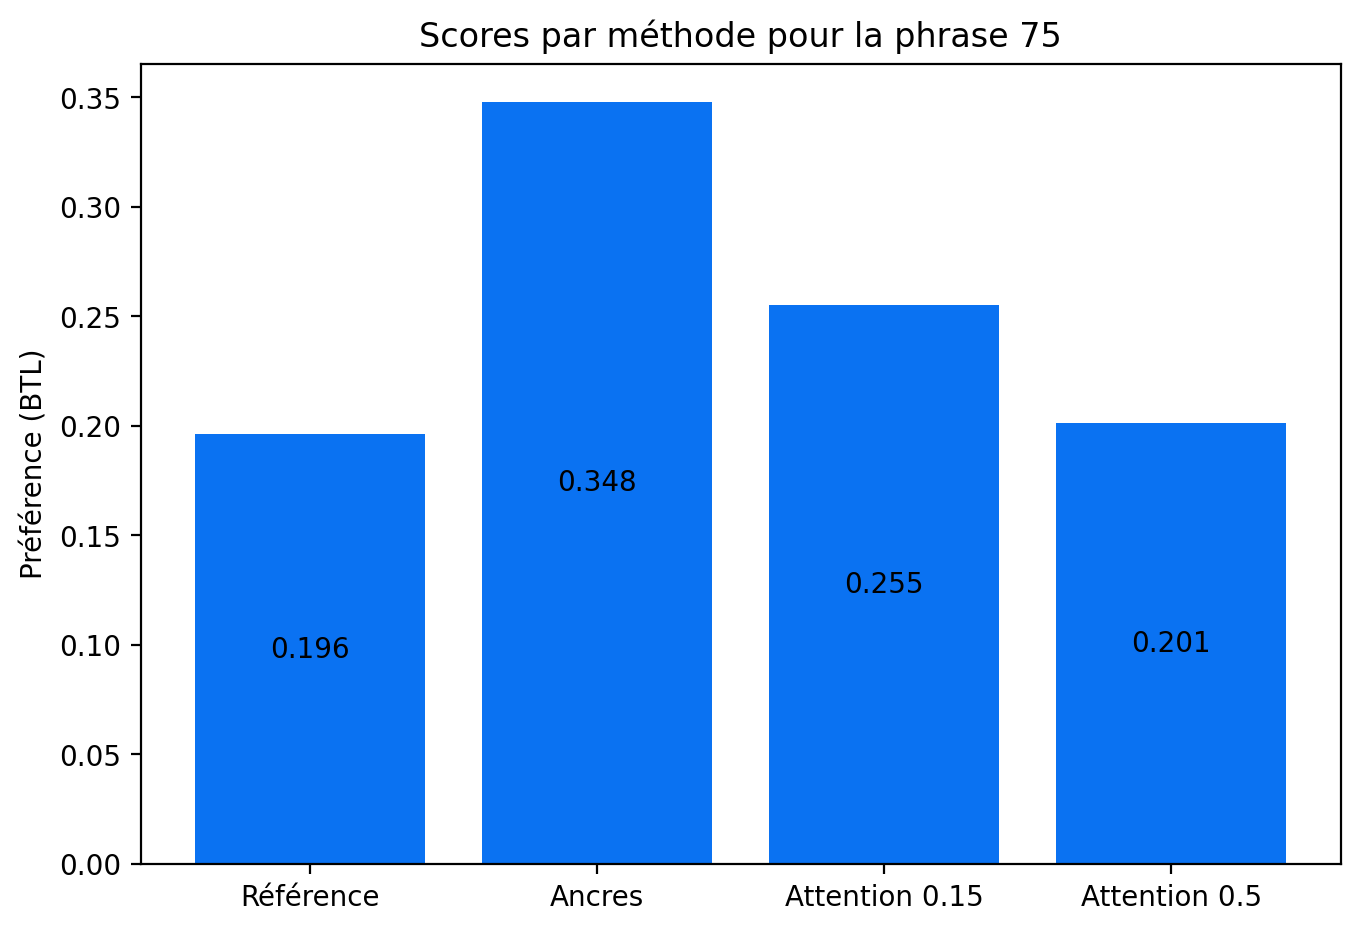
\includegraphics[width=0.68\textwidth]{S3-Comparaison_de_methodes/figures/btl_plot.png}
  \caption{Exemple des scores obtenus avec le modèle BTL pour chaque méthode d'explication sur une phrase du jeu de données LEGO - DE. La valeur correspond à la probabilité qu'un utilisateur préfère une méthode plutôt que les autres. L'explication humaine correspond à la colonne ``Référence''. }\label{fig:btl_plot}
 \end{center}
\end{figure}

Nous observons ensuite les scores BTL sur l'ensemble du jeu de données LEGO DE, et sur deux sous-ensembles : les vrais positifs et les faux positifs, car nous nous attendons à ce que les résultats diffèrent. Les résultats sont comparés dans la figure~\ref{fig:btl_plot_global}. Cette analyse ne montre aucune différence significative entre les méthodes, autant sur la base complète que sur les deux sous-ensembles. Un tel résultat souligne que, sur le plan global, aucune méthode ne l'emporte en termes de préférence utilisateur.

\begin{figure}[h!tpb]
  \setlength{\belowcaptionskip}{-20pt}
 \begin{center}
  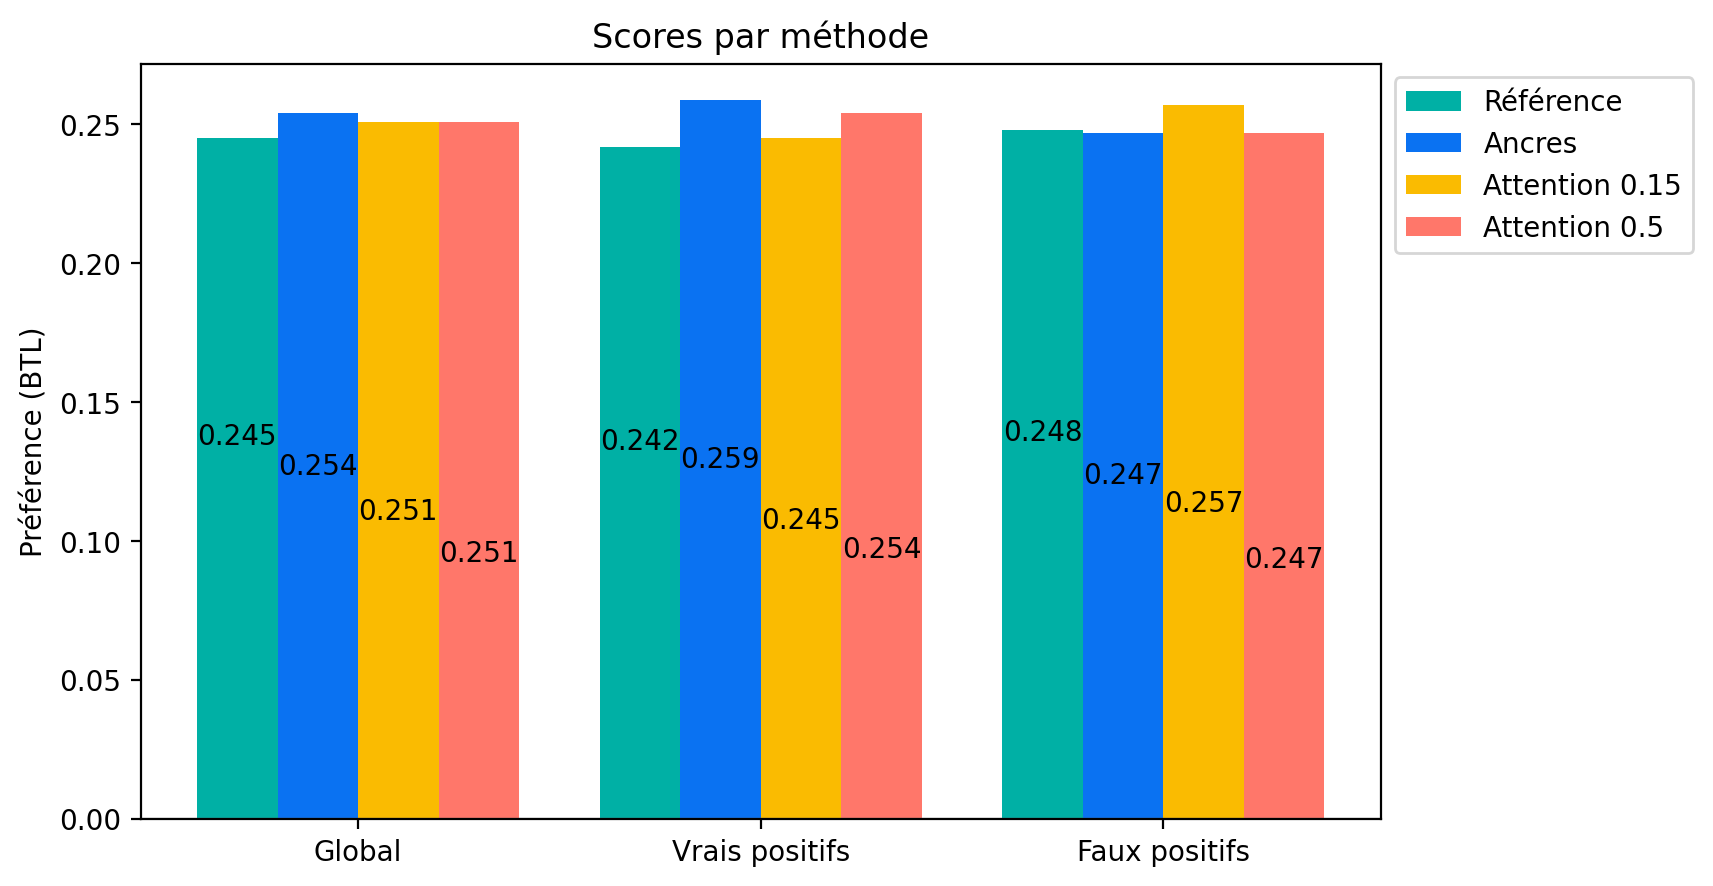
\includegraphics[width=0.9\textwidth]{S3-Comparaison_de_methodes/figures/btl_plot_global_tp_fp.png}
  \caption{Scores obtenus avec le modèle BTL pour chaque méthode d'explication, sur le jeu de données LEGO DE. Les vrais positifs et les faux positifs sont indiqués. Aucune différence significative n'apparaît entre les méthodes.}\label{fig:btl_plot_global}.
 \end{center}
\end{figure}

Comme nous l'avons fait dans la section~\ref{C3:iou_lego_de}, nous allons diviser notre ensemble de données par phrases avec des explications de référence \textit{vide}, \textit{simple} et \textit{complexe}. L'algorithme BTL nous donne l'échelle psychométrique associée dans la Figure~\ref{fig:btl_plot_cplx}.

\begin{figure}[h!tpb]
  \setlength{\belowcaptionskip}{-20pt}
 \begin{center}
  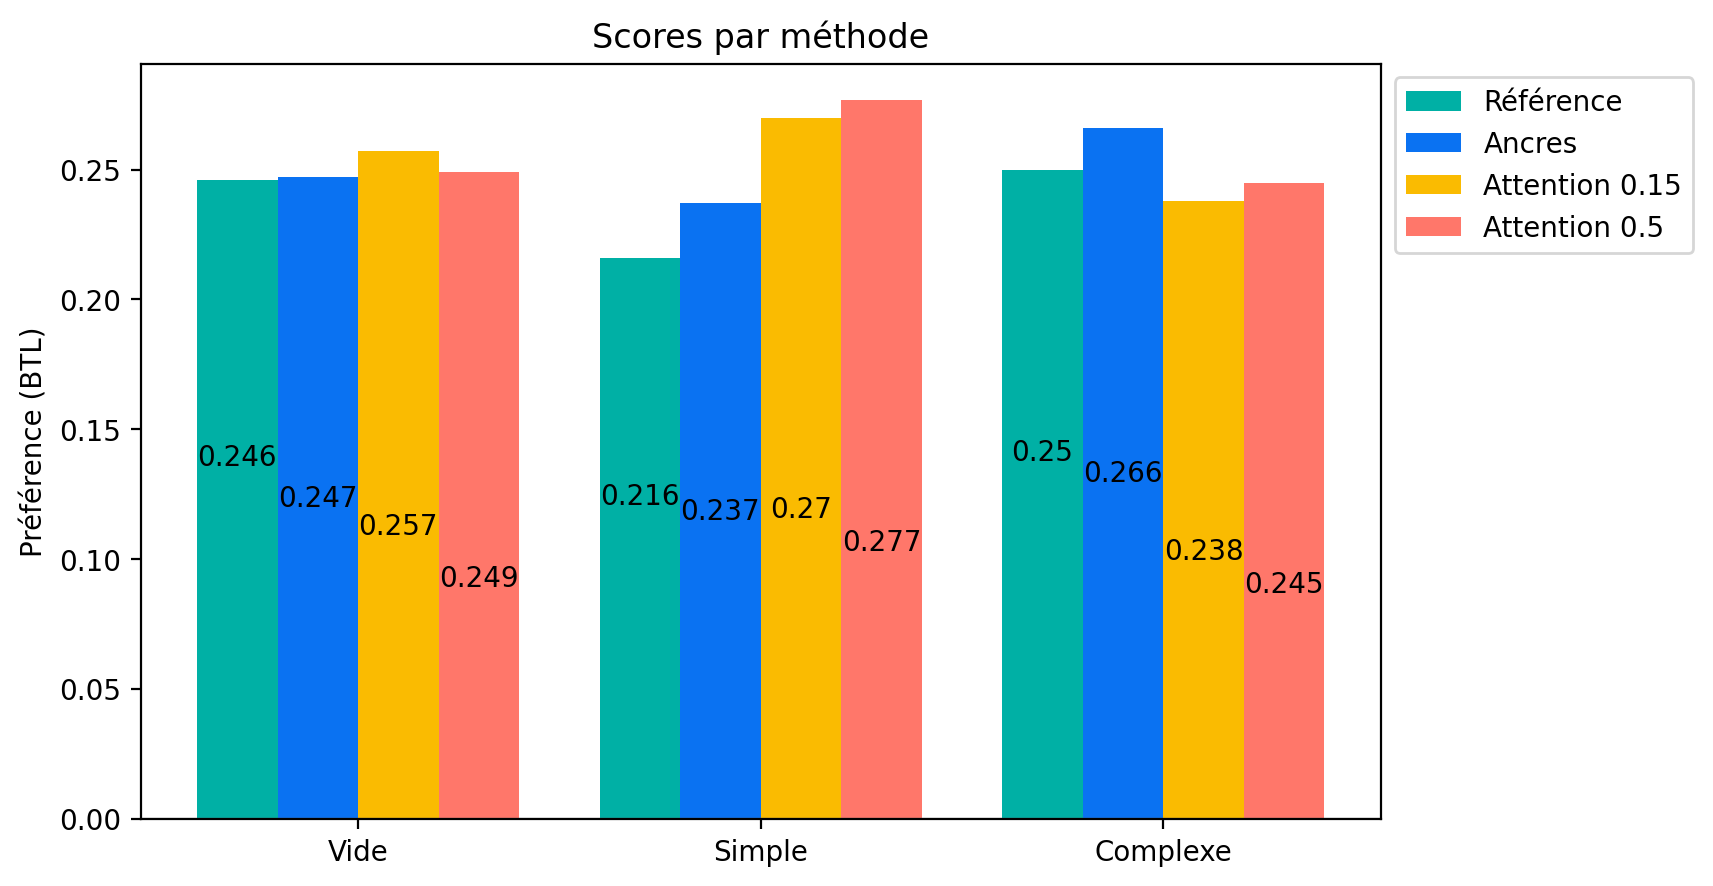
\includegraphics[width=0.9\textwidth]{S3-Comparaison_de_methodes/figures/btl_by_complexity.png}
  \caption{Scores obtenus avec le modèle BTL pour chaque méthode d'explication, sur le jeu de données LEGO DE, par complexité. Ce regroupement montre des différences dans les préférences des utilisateurs. }\label{fig:btl_plot_cplx}
 \end{center}
\end{figure}

Encore une fois, cette échelle psychométrique peut être transformée en podiums, affichés dans le tableau~\ref{pus_podium}. Faisons la première analyse pour tous les types de phrases. Pour les phrases avec une explication de référence vide, les utilisateurs n'ont pas une forte préférence pour une méthode ou une autre, comme le montre la Figure~\ref{fig:btl_plot_cplx}. Le podium dans le tableau~\ref{pus_podium} indique que la légère préférence va aux méthodes d'attention.
Pour les cas simples, les méthodes d'attention interne sont préférées, et l'explication humaine est la moins appréciée. Pour les cas plus complexes, la méthode d'explication des ancres a été préférée, et les méthodes d'attention interne sont en difficulté. Dans notre cas d'usage, en d'autres termes, les utilisateurs préfèrent les méthodes d'attention dans les cas simples. Lorsque les choses deviennent plus complexes, leur préférence va à la méthode d'explication des ancres.

\begin{table}[h!tpb]
    \centering
    \addtolength{\parskip}{-0.5mm}
  \caption{Podium basé sur une étude psychométrique des utilisateurs, sur le jeu de données LEGO DE, par catégorie d'explication.} \label{pus_podium}
  \begin{tabular}{|l|l|p{0.25\textwidth}|l|l|}
      \hline
           & \textbf{Premier}& \textbf{Second}   & \textbf{Troisième} \\ \hline
  Vide     &  Attention 0,15 &  (Attention 0,5 ,  Ancre , Référence)  &&   \\ \hline
  Simple   &  Attention 0,5  &  Attention 0,15     & Ancre      &   Référence    \\ \hline
  Complexe &  Ancre          & Référence      &  Attention 0,5      &   Attention 0,15      \\ \hline
  \end{tabular}
  \end{table}

% Conclusion et transition
Nous avons calculé les préférences de chaque méthode d'explication et établi des podiums. L'analyse des résultats montre que différentes catégories de phrases existent et amènent des différences dans les préférences utilisateurs. Les podiums ainsi obtenus par catégorie sont comparés aux podiums de la métrique qualitative dans la section suivante.

\subsection{Résultats} \label{C3:pus_result}

% Quoi
Nous pouvons maintenant comparer les résultats de l'analyse quantitative de la section~\ref{C3:qt_metric} et les préférences des utilisateurs.
% Comment
Comme nous l'avons fait précédemment, nous regroupons les phrases par la complexité des explications de référence selon trois groupes : explications \textit{vides}, \textit{simples}, et \textit{complexes}.
Nous souhaitons désormais savoir si les méthodes d'explication qui performent le mieux sont également celles préférées par les humains.

% résultats
Les podiums du Tableau~\ref{qtm_podium} et du Tableau~\ref{pus_podium} présentés dans les sections précédentes diffèrent fortement. En effet, la métrique de similarité est basée sur les explications humaines en tant que référence, qui n'est pas la méthode préférée des utilisateurs.
Le diagramme à barres empilées tel qu'indiqué dans la Figure~\ref{fig:iou_btl_e} permet de comparer la proportion relative des méthodes dans chaque cas. Les valeurs de similarité par IOU sont normalisées pour la comparaison, afin que la somme de tous les scores soit égale à un. Les valeurs réelles sont présentées dans le tableau~\ref{iou_lego_de_cplx}.

Pour les phrases de catégorie \textit{vides}, la figure~\ref{fig:iou_btl_e} montre que l'IOU et BTL reflètent des explications différentes. Pour rappel, le jeu de données DE est composé de phrases étiquetées comme non conformes par notre modèle. Les explications de référence vides sont associées à des phrases conformes, qui ont été prédites à tort comme non conformes par le modèle. Dans ce cas, les explications humaines telles que nous les avons définies peuvent ne pas être la bonne référence pour calculer les IOU. Comme expliqué dans la section~\ref{C2:ground_truth}, les experts du domaine pourraient préférer une explication attendue, qui devrait être définie pour un modèle spécifique.

\begin{figure}[h!tpb]
  \setlength{\belowcaptionskip}{-0pt}
 \begin{center}
  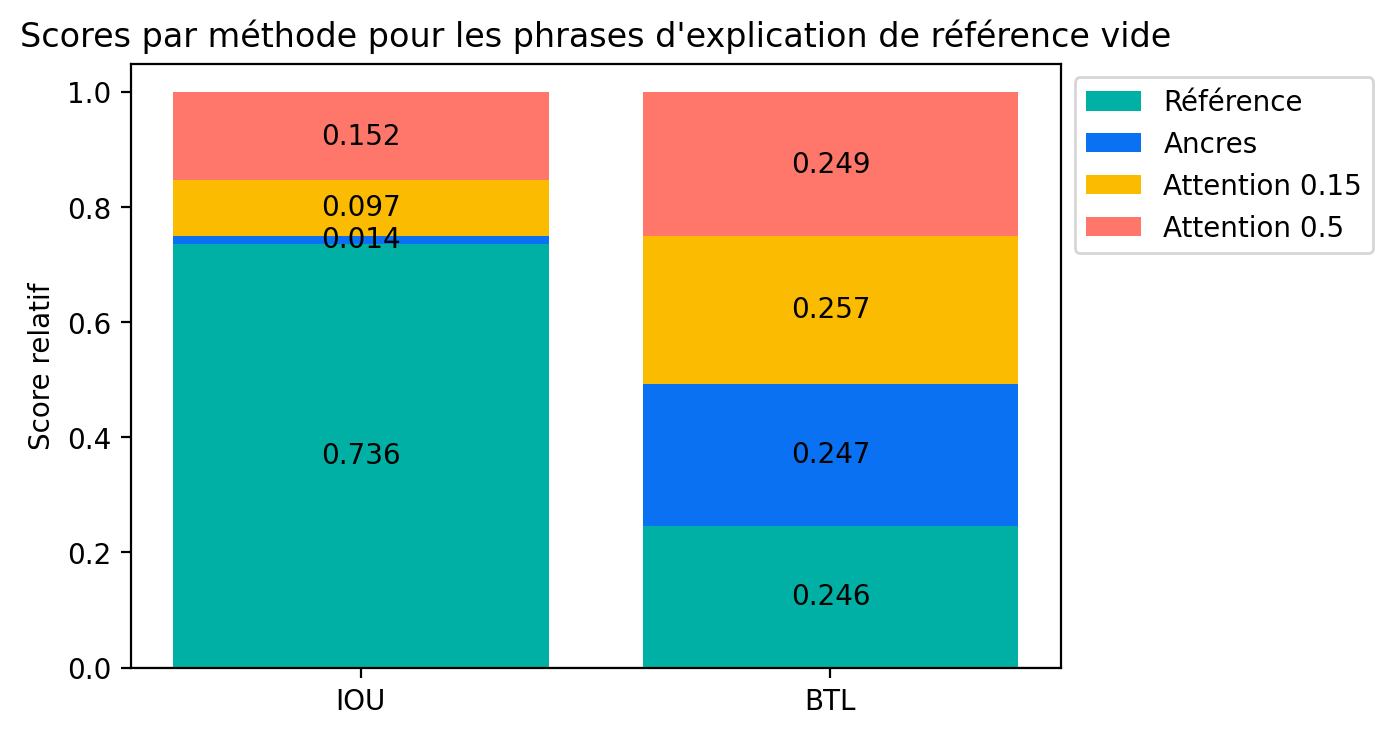
\includegraphics[width=0.8\textwidth]{S3-Comparaison_de_methodes/figures/iou_btl_e.png}
  \caption{Scores relatifs de similarité (IOU) et de préférence (BTL) normalisés pour chaque méthode d'explication, sur le jeu de données LEGO DE, filtré sur les phrases avec des explications vides. }\label{fig:iou_btl_e}
 \end{center}
\end{figure}

Le cas des phrases associées à des explications humaines \textit{simples} est présenté dans la figure~\ref{fig:iou_btl_s}. Elle met en évidence de bons résultats quantitatifs pour l'\textit{attention 0,15} et les ancres, l'\textit{attention 0,5} étant la méthode qui correspond le moins à l'explication humaine. Les utilisateurs n'ont pas préféré l'explication humaine aux autres méthodes et ont préféré l'\textit{attention 0,5}. Prendre l'explication humaine comme référence n'a donc pas de sens, et nous pouvons en conclure que l'IOU basée sur l'explication humaine n'est pas efficace ici non plus. Cependant, les utilisateurs semblent apprécier les explications courtes, puisqu'iels ont préféré \textit{attention 0,5} à \textit{attention 0,15}. Notre métrique quantitative devrait refléter ce point, en diminuant lorsque la longueur d'une explication augmente.

\begin{figure}[h!tpb]
  \setlength{\belowcaptionskip}{-20pt}
 \begin{center}
  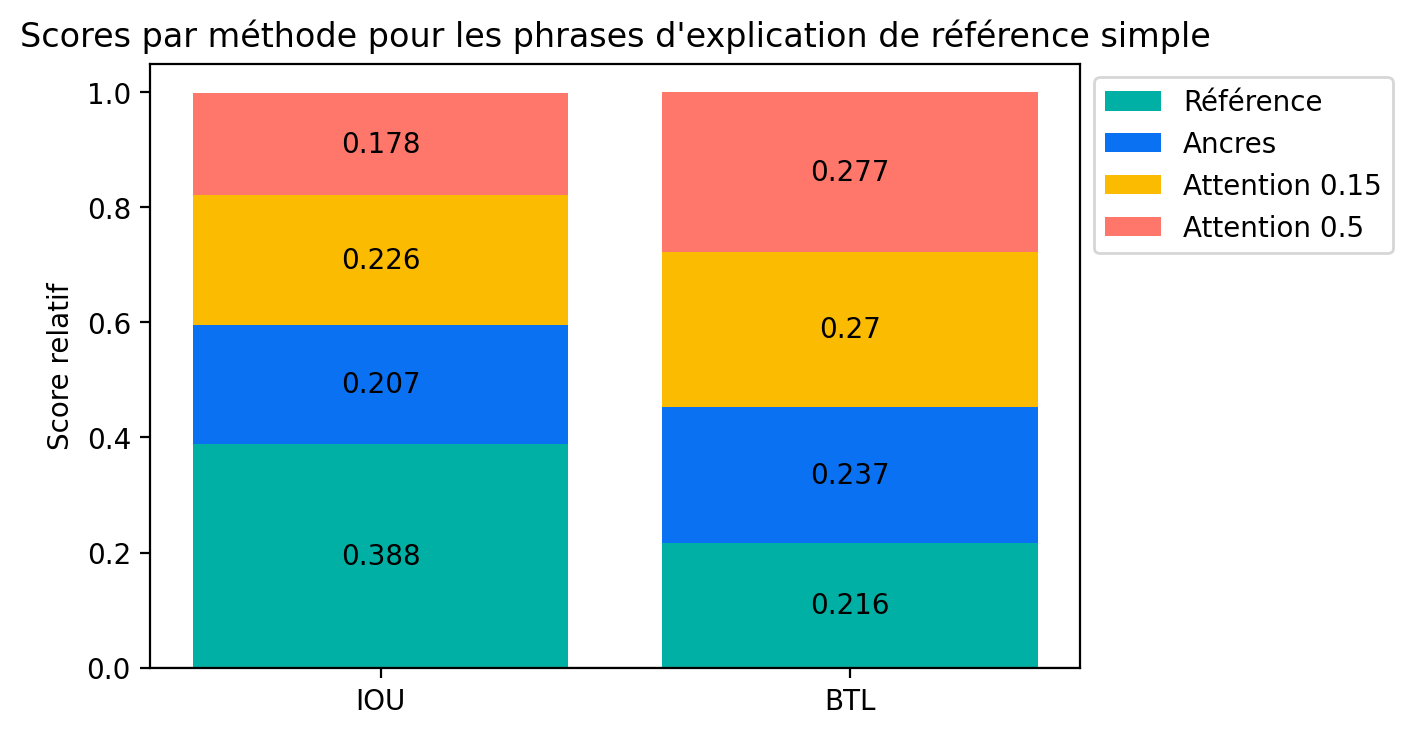
\includegraphics[width=0.8\textwidth]{S3-Comparaison_de_methodes/figures/iou_btl_s.png}
  \caption{Scores relatifs de similarité (IOU) et de préférence (BTL) normalisés pour chaque méthode d'explication, sur le jeu de données LEGO - DE, filtré sur les phrases avec des explications simples. Les explications de référence sont d'IOU égale à $1$ avant normalisation.  }\label{fig:iou_btl_s}
 \end{center}
\end{figure}

Les podiums pour les phrases avec des explications de référence plus complexes sont comparés dans la figure~\ref{fig:iou_btl_c}. L’IOU montre une bonne correspondance pour les explications des ancres. Cela se reflète dans l'étude des utilisateurs, puisque la méthode préférée est celle des ancres, suivie de la référence. En considérant l’IOU, l'\textit{attention 0.5} est moins performante comparée à \textit{attention 0.15}. Cependant la préférence des utilisateurs est inverse. Comme l'\textit{attention 0,5} est un sous-ensemble de \textit{attention 0,15}, cela indique une préférence pour les explications plus courtes. Tout comme pour les cas simples, notre métrique refléterait mieux les préférences des utilisateurs en tenant compte de la longueur des explications.

\begin{figure}[h!tpb]
  % \setlength{\belowcaptionskip}{-20pt}
 \begin{center}
  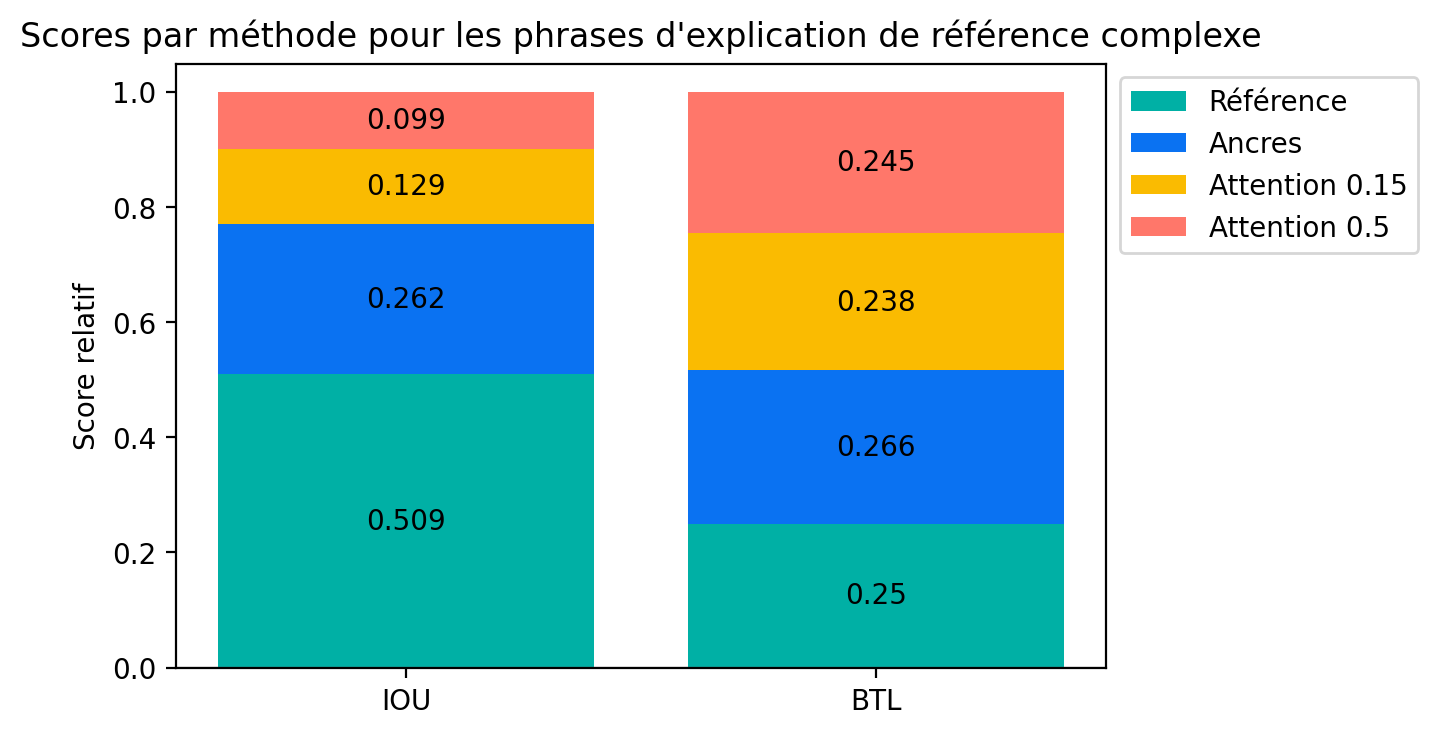
\includegraphics[width=0.8\textwidth]{S3-Comparaison_de_methodes/figures/iou_btl_c.png}
  \caption{Scores relatifs de similarité (IOU) et de préférence (BTL) normalisés par méthode d'explication, sur le jeu de données LEGO DE, filtré sur les phrases avec des explications complexes. }\label{fig:iou_btl_c}
 \end{center}
\end{figure}

Pour toutes ces catégories, nos podiums sont différents. Selon notre protocole, cela signifie que notre mesure quantitative ne reflète pas la préférence humaine. Pour ajuster cette mesure, l'analyse des résultats donne deux pistes.
\begin{itemize}
    \item Les explications attendues sont plus pertinentes que les explications idéales (Cf. section~\ref{C2:ground_truth}) pour mesurer la préférence des utilisateurs.
    \item Prendre en compte la préférence des utilisateurs pour les explications courtes.
\end{itemize}
Nous répondons à notre seconde question : ``comment faire pour que la métrique quantitative corresponde aux préférences des utilisateurs?'' par une nouvelle mesure de performance.
% \begin{equation}\label{qtm_iou}
%   metrique = \frac{e_{generee} \cap e}{e_{ideale} \cup e}
% \end{equation}
% à
\begin{equation}\label{qtm_new}
  performance = \frac{e_{generee} \cap e}{e_{attendue} \cup e} \frac{\alpha}{len(e)}
\end{equation}

\section{Conclusion}

% Objectif  du chapitre
Nous avons collecté en section~\ref{C3:test_u} les retours des utilisateurs dans la conception des systèmes d'explications. Nous avons ensuite présenté les comparaisons de méthodes de génération d'explications, dans deux contextes : sans utilisateurs en section~\ref{C3:iou_expe} et avec en section~\ref{C3:pus}. Les protocoles ont été conçus pour être généralisés à tout cas d'usage de classification multi-classe. Ils sont applicables à toute méthode d'explication par variable d'importance.

% on en retire quoi, limites
Le test d'utilisabilité a donné l'idée d'une interface non envisagée avant : l'explication par la règle. Il a démontré son intérêt tout en nécessitant peu de temps de réalisation.

La comparaison sans utilisateurs donne des résultats différents selon le cas d'usage.
Pour le second protocole, les résultats montrent que la méthode préférée dépend de la taille de l'explication de référence. Les explications de référence ne sont pas représentatives des préférences des utilisateurs. Les utilisateurs préfèrent des explications courtes.

Cette mise en pratique met en lumière la dépendance de ces méthodes d'évaluation à la disponibilité et la qualité d'explications de référence. Sans ces explications les évaluations sont restreintes et nécessitent une analyse manuelle qui, bien que rendue la plus efficiente possible, reste lourde.
Les faux positifs sont une source de différence entre les explications attendues et les explications idéales, et cibler ceux-ci peut réduire le coût de passer d'explications idéales à attendues.

% et on discute de la suite
Nous avons évalué le format et les méthodes de génération d'explications locales. Dans le chapitre suivant, nous nous attelons à générer des explications globales sur le comportement d'un modèle.

\boitemagique{Résumé}{
\begin{itemize}
    \item[\checkmark] Nous avons collecté les besoins des experts du domaine
    \item[\checkmark] Les systèmes d'explications les plus complexes ne mènent pas aux interfaces les plus appréciées des utilisateurs
    \item[\checkmark] L'évaluation des explications sans avis humain permet une première mesure de d'adéquation
    \item[\checkmark] L'évaluation subjective permet de tenir compte les préférences des experts dans la mesure de performance
    \item[\checkmark] Le protocole d'évaluation a mené aux publications~\cite{Jouis2021,Jouis2021a,Jouis2023}
\end{itemize}
}


\clearemptydoublepage
\chapter[Caractérisation d'un modèle d'Intelligence Artificielle]{Caractérisation d'un modèle d'Intelligence Artificielle}

\boitemagique{Dans ce chapitre}{
Ce chapitre propose une méthode de caractérisation globale d'un modèle. L'objectif est de construire une représentation mentale du modèle. Un extrait pertinent de paires d'exemples de contre-exemples proches.
La stratégie puis l'implémentation de la méthode sont présentées. L'application met en avant les avantages et limites de la proposition.
Cette méthode de caractérisation est prometteuse, mais reste à comparer à d'autres méthodes de la littérature.
}

% Avant
Nous avons présenté dans les chapitres précédents des explications locales.
Dans ce chapitre, nous caractérisons globalement un modèle d'IA.
Ce chapitre répond à des besoins d'auditabilité et des contraintes légales.
% Objectif
Notre objectif est de permettre aux utilisateurs de créer un modèle mental fidèle au modèle caractérisé. La notion de \textit{modèle mental} est introduite en section~\ref{C1:generation}.
% comment
Nous proposons une méthodologie générale de caractérisation, qui s'appuie sur les limites de décision par classe d'un modèle d'IA

% Résultats
Nous présentons notre protocole et l'appliquons à un cas d'utilisation réel dans le domaine du traitement du langage naturel.
L'application montre son potentiel sur l'une des classes d'un modèle de classification. L'analyse de l'explication permet d'appréhender des éléments clés de la frontière de décision, et d'émettre des hypothèses d'amélioration du jeu de données d'entraînement.
Nous notons également des marges d'amélioration. Ainsi l'ajout d'une méthode d'explication locale est nécessaire pour l'analyse des textes longs.

% plan
Nous présentons en section~\ref{C4:strategie} la méthode de caractérisation, et son implémentation en section~\ref{C4:implémentation}. Enfin, nous appliquons cette caractérisation en section~\ref{C4:application}.



\section{Stratégie}  \label{C4:strategie}
%  quel type d'explication, quel besoin, dans quel contexte, quelle méthode pour y répondre
Nous nous  intéressons au contexte de la classification multi-label, multi-classes.
Dans le chapitre~\ref{C1}, nous présentons Lime, méthode d'explication locale, et son explication globale associée : SP-Lime~\cite{Ribeiro2016}. Cette explication globale s'appuie sur des exemples dont l'explication Lime a été réalisée au préalable. Elle est donc coûteuse. Toutefois, c'est cette philosophie qui conduit la suite des travaux présentés dans ce chapitre.

% Afin de permettre à l'utilisateur de créer son modèle mental, le modèle est décrit classe par classe.
Comment permettre à l'utilisateur d'avoir un modèle mental fidèle au comportement réel du modèle original (MO) ? Pour résoudre cette problématique, nous proposons d'aider à l'appréhension des frontières de décision du MO. Cette aide se traduit par l'analyse d'un ensemble limité d'exemples et de contre-exemples pour une classe donnée, comme illustré avec le tableau~\ref{tab:illus_e_cfe}. Un exemple, dans la première colonne du tableau, correspond ici à la classe étudiée et un contre-exemple, dans la seconde colonne, est un élément d'une autre classe. L'ensemble des couples d'exemple et contre-exemple permet d'appréhender différents aspects d'une classe, notamment ses frontières avec d'autres classes. Les exemples situés au c\oe ur d'une classe nous semblent moins pertinents.

% Qu'est-ce que je présente à l'utilisateur ?
\begin{table}[htpb!]
    \caption{Délimitation de la classe \textit{``Discrimination : Contrat étudiant''}  sous la forme d'exemples et contre-exemples associés} \label{tab:illus_e_cfe}
    \begin{tabular}{|p{0.45\textwidth}|p{0.50\textwidth}|} \hline
    \textbf{Exemple type}                                            & \textbf{Contre-exemple associé}     \\ \hline
    Profil recherché: Etudiant(e), salarié(e), retraité(e). & Etudiant(e), retraité(e), travaillant à temps partiel ou   en recherche d'emploi, vous êtes avant tout passionné(e) par les enfants? \\ \hline
    Etudiants acceptés.                                     & 35 H/Semaine minimum Etudiants acceptés. \\ \hline
    \end{tabular}
\end{table}

Un utilisateur ne peut recevoir un nombre trop important d'éléments à traiter à la fois. Ces exemples doivent donc être habilement sélectionnés. Illustrée en figure~\ref{fig:strategie}, notre stratégie consiste à prendre un ensemble d'exemples candidats, puis de filtrer et trier les exemples qui en sont issus. Le filtre vise à conserver uniquement les exemples qui ont une pertinence technique pour représenter le comportement du MO. Il est possible que le filtre ne suffise pas pour montrer un ensemble restreint d'une dizaine d'éléments à un utilisateur ou une utilisatrice. Un tri est alors effectué avec pour but de proposer un résumé digeste et représentatif pour l'utilisateur. Ce tri peut être laissé à la main de l'utilisateur.

\begin{figure}[h!tpb]
 \centering 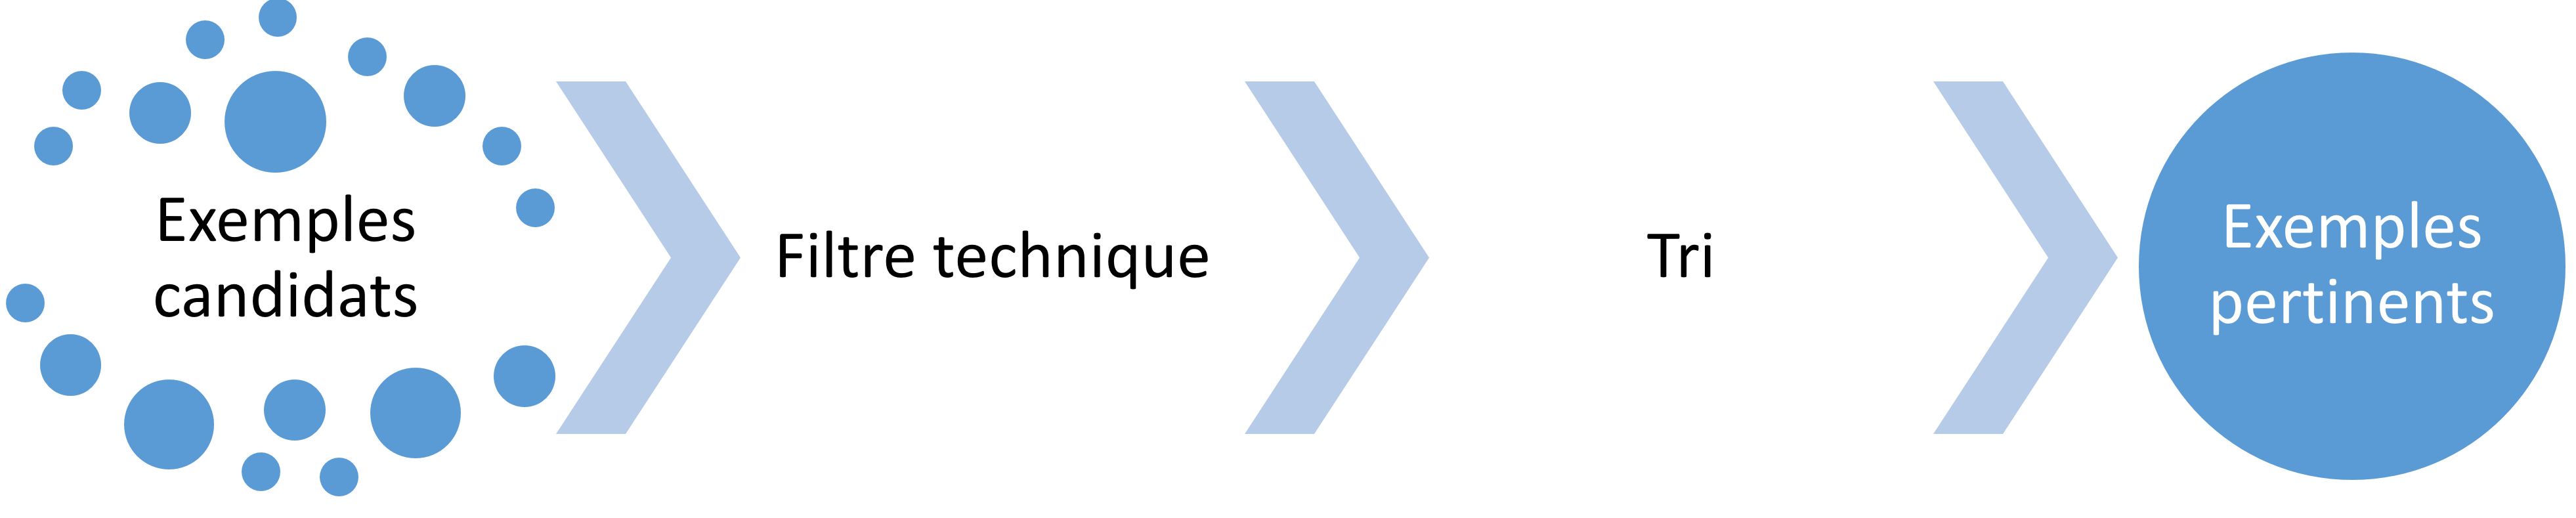
\includegraphics[width=0.9\textwidth]{S4-Explicabilite_globale/figures/strategie.png}
\caption{La stratégie de sélection des exemples à présenter à l'utilisateur.} \label{fig:strategie}
\end{figure}

La figure~\ref{fig:strategie} présente l'enchainement de définition d'exemples candidats, filtre, et tri de ces exemples. Les détails sont volontairement mis de côté, nous proposons une méthodologie générale dont les implémentations des différents éléments sont à adapter.

% Transition
Maintenant que nous avons défini ce que nous souhaitons présenter aux utilisateurs, et la stratégie générale, nous pouvons définir l'implémentation de cette stratégie.

\section{Implémentation} \label{C4:implémentation}

Dans cette section, nous présentons cette implémentation ainsi que nos choix techniques.
Tous les éléments présentés ici sont des choix d'implémentation qui ne sont pas fixés. Il est possible de modifier les trois étages présentés ici, en conservant la structure présentée en section précédente.
Nous proposons cette première solution fonctionnelle, appliquée sur un cas d'usage en section~\ref{C4:application}. Celle-ci reste à évaluer, et adapter à d'autres situations et contraintes.

 Nous présenterons en premier lieu la sélection d'un ensemble d'exemples candidats en section~\ref{C4:candidats}. En section~\ref{C4:filtre} nous détaillerons le filtre technique effectué, et en section~\ref{C4:tri} le tri appliqué.

\subsection{Choix de la source d'exemples candidats} \label{C4:candidats}

Les exemples présentés aux utilisateurs dans la littérature peuvent être issus des données réelles, comme dans~\cite{Ribeiro2016}. Les candidats sont alors les données d'entraînement, de développement et de test. Ces exemples peuvent également être générés. Dans~\cite{Charachon2021}, les auteurs créent des explications sous la forme de la différence entre des exemples et contre-exemples générés. Les techniques de génération actuelles permettent de créer des données complexes telles que des textes~\cite{Wang2021} et images~\cite{Ramesh2022}.

Générer les exemples et contre-exemples nécessite un apprentissage supplémentaire du modèle générateur, et crée des données non connues par le MO. L'entraînement d'un modèle générateur ajoute une technique d'apprentissage profond. Cette méthode a pour risque de reporter le problème d'explication à ce nouveau modèle générateur. Afin de réduire les efforts des utilisateurs pour reconstruire leur modèle mental, nous nous appuyons sur des exemples candidats concrets.
Nous préférons nous appuyer sur les données issues de la base d'apprentissage, permettant ainsi de ne pas s'appuyer sur une couche supplémentaire d’apprentissage profond. Nous nous assurons aussi d'avoir uniquement des données réelles, nécessitant en contrepartie d'avoir accès au jeu de données d'entraînement.

Toutes les données d'entraînement n'ont pas le même impact sur le comportement du modèle. Comme défini en section~\ref{C4:strategie}, nous souhaitons conserver, parmi les exemples candidats, uniquement ceux qui ont une pertinence du point de vue du MO.

\subsection{Filtre} \label{C4:filtre}

Ces exemples pertinents sont ceux qui représentent le fonctionnement du MO. Nous cherchons notamment les données présentes aux frontières de décision, qui pourraient être récupérées en filtrant les données d'apprentissage qui en sont proches.

% Approche centrée NN
Pour déterminer ces points, différentes approches existent. Nous pouvons par exemple nous appuyer sur le fonctionnement d'un réseau de neurones. Les points dont le score de prédiction (sortie du MO) est proche de 0,5 pour une classe donnée correspondent à des points qui ne sont pas typiques de cette classe. Cependant, il est plus difficile de dire si ces points sont situés près d'une frontière ou s'ils ont un score faible car ils sont hors de la distribution des données ou aberrants.

% Approche sur les données
Il est également possible de prendre des points antagonistes (de classes différentes) proches  d'une manière centrée sur les données.
En définissant une fonction de distance entre les points, nous pouvons sélectionner le couple de points les plus proches qui appartiennent à deux décisions de modèle différentes comme antagonistes. Mais ces points peuvent ne pas être les plus représentatifs de la frontière de décision. Dans un contexte de classification One \textit{vs.} Rest, plusieurs couples d'instances de données peuvent être nécessaires pour bien définir la frontière de décision. Dans un mode One \textit{vs.} One, si deux classes sont éloignées dans l'espace de représentation, le couple d'instances de données résultant n'aura aucun intérêt. Certaines frontières complexes nécessitent également la définition de plus d'un couple d'exemples.

Nous proposons un filtre basé sur les SVM pour extraire les exemples factuels et contrefactuels pertinents. Le filtre s'appuie sur la notion de vecteurs supports du SVM, soit les points de données importantes pour l'apprentissage du SVM. Il est composé de 3 étapes : suppression des doublons, sélection des vecteurs supports et appairage.
% TODO Harold : ajouter un argumentaire :
% - classifieur fortement discriminant permettant de se focaliser sur les frontières
% - se base sur les données d'apprentissage pour la définition du modèle ( les vecteurs supports)
% - utilisation de noyaux gaussiens pour retrouver un pouvoir génératif ( on peut retrouver les données utilisées)
% - un seul paramètres pour choisir le compromis de complexité biais/variance: C
\begin{figure}[h!tpb]
    \begin{subfigure}[t]{0.45\textwidth}
      \centering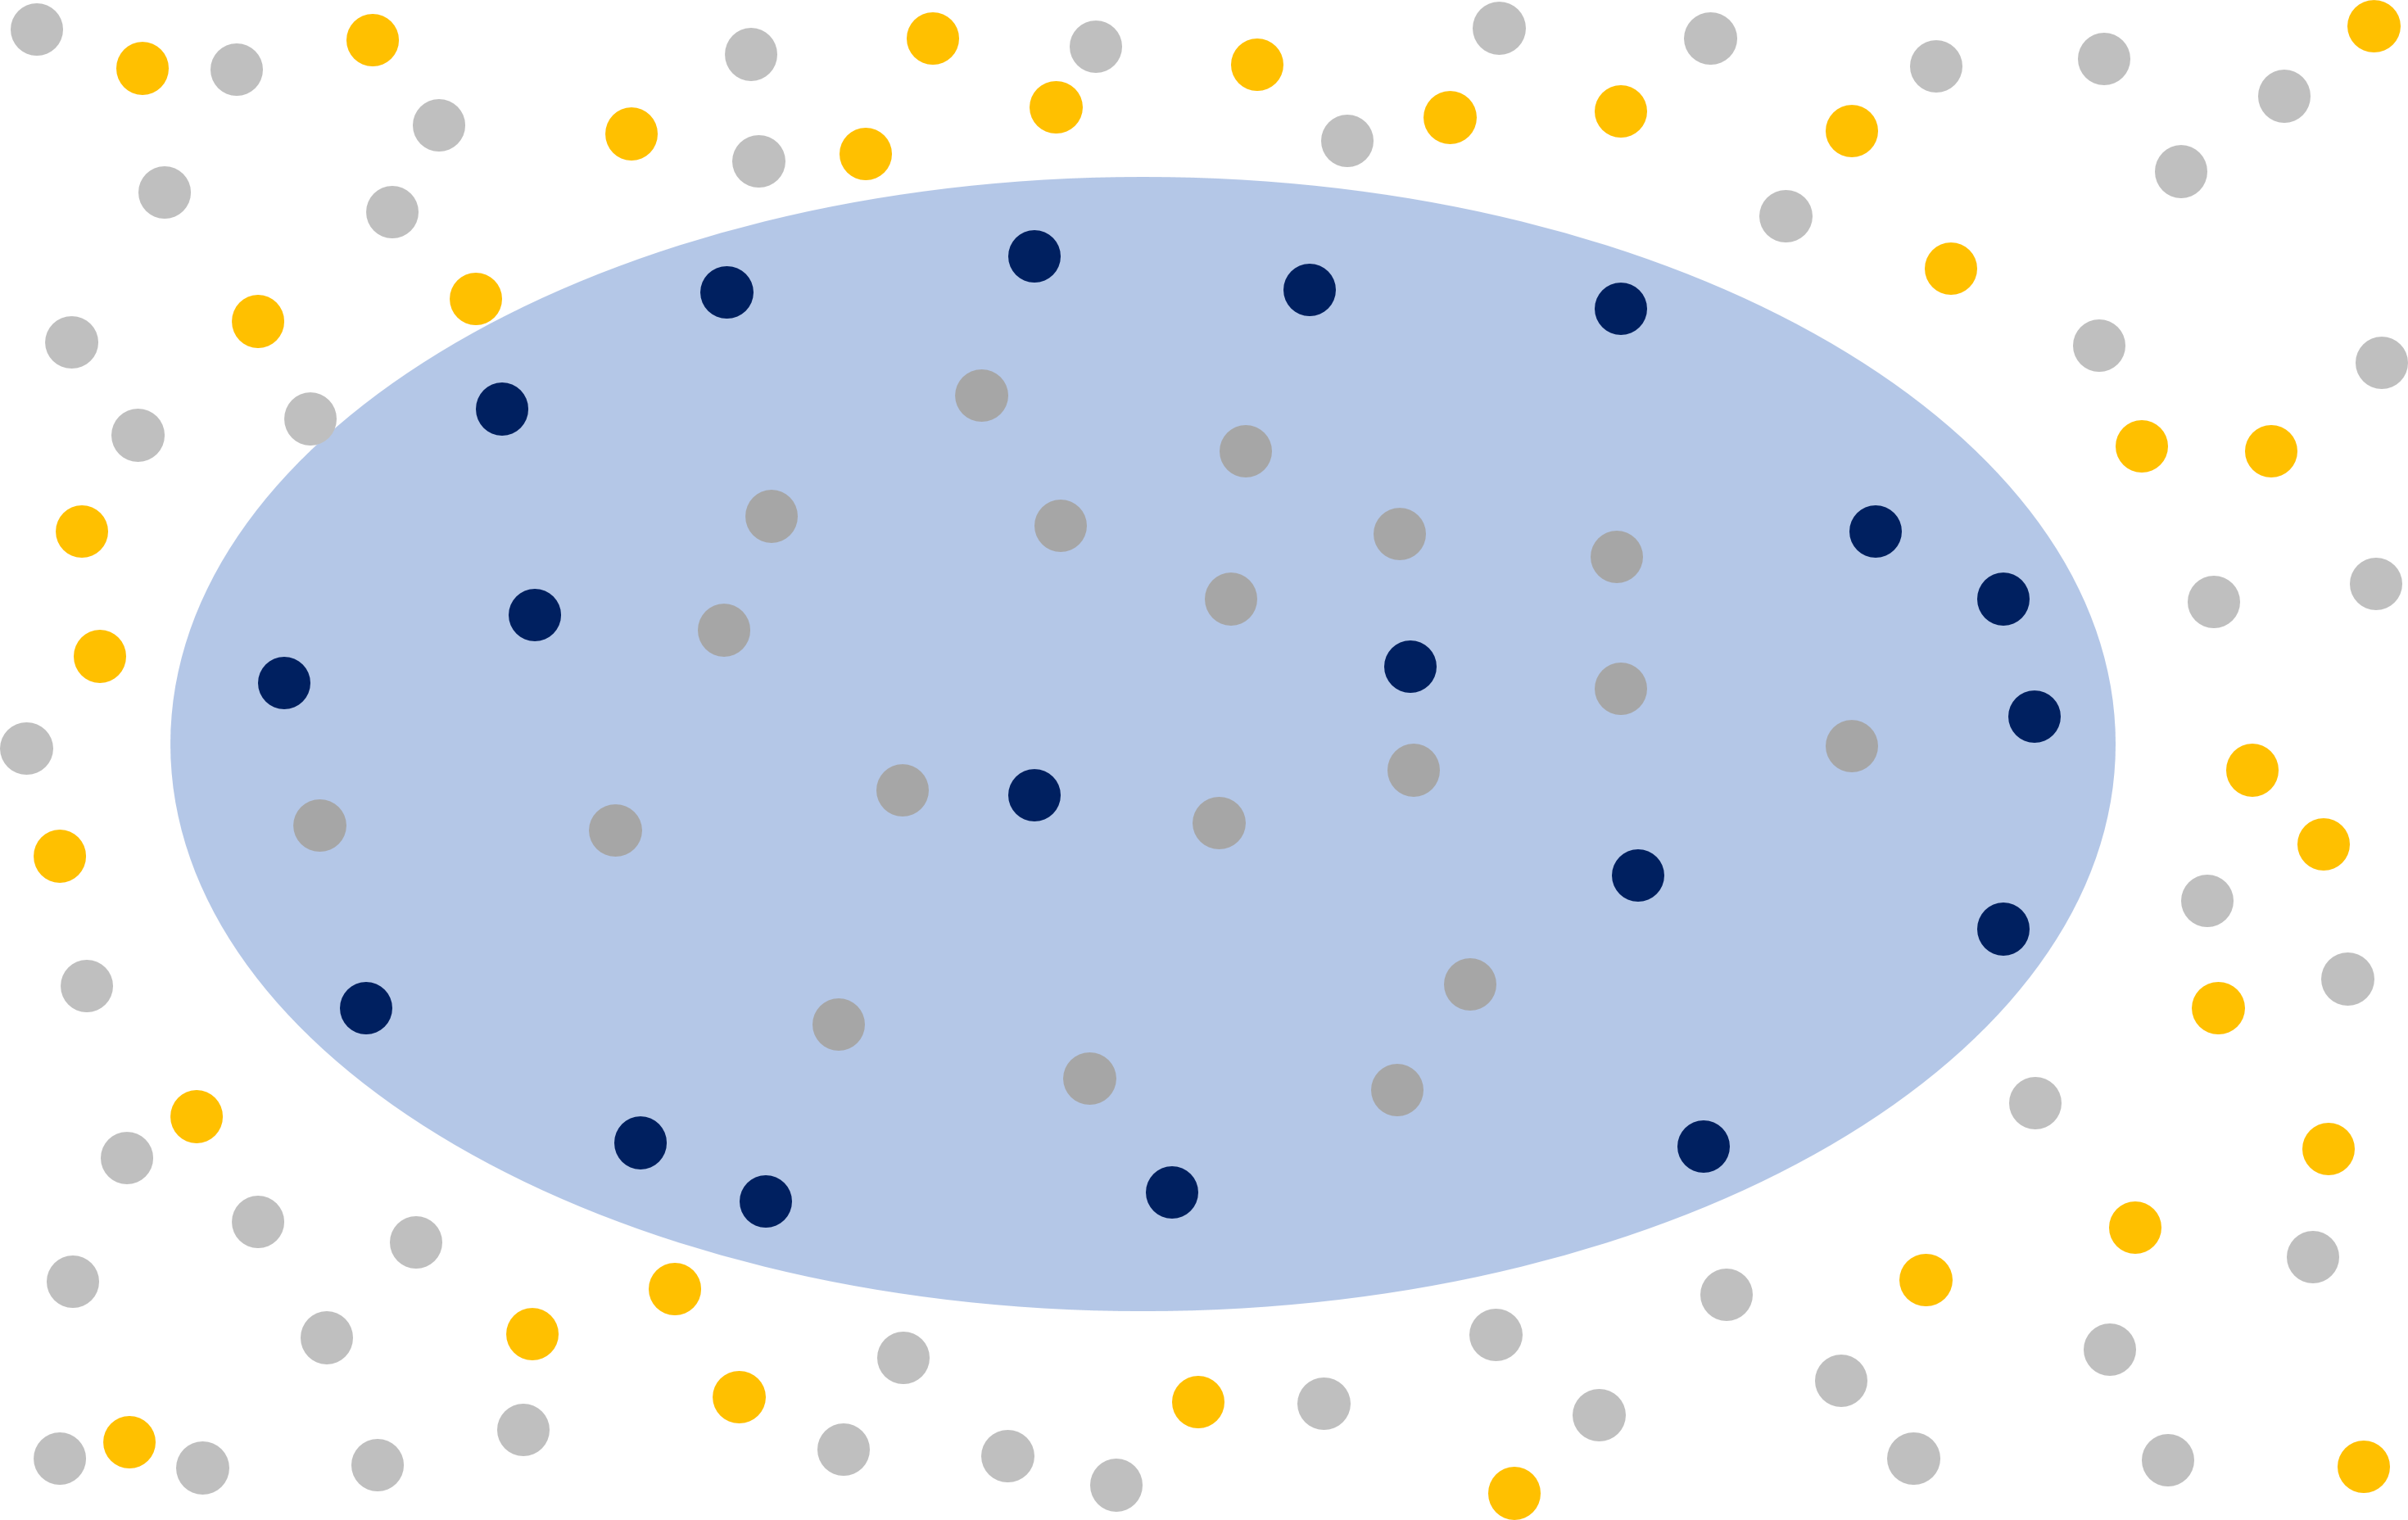
\includegraphics[width=\textwidth]{S4-Explicabilite_globale/figures/filtre1.png}
      \caption{Les données candidates. Les points bleus et jaunes correspondent aux vecteurs supports protagonistes et antagonistes. Les autres points de données sont en gris}  \label{fig:filtre1}
    \end{subfigure} \qquad
    \begin{subfigure}[t]{0.45\textwidth}
      \centering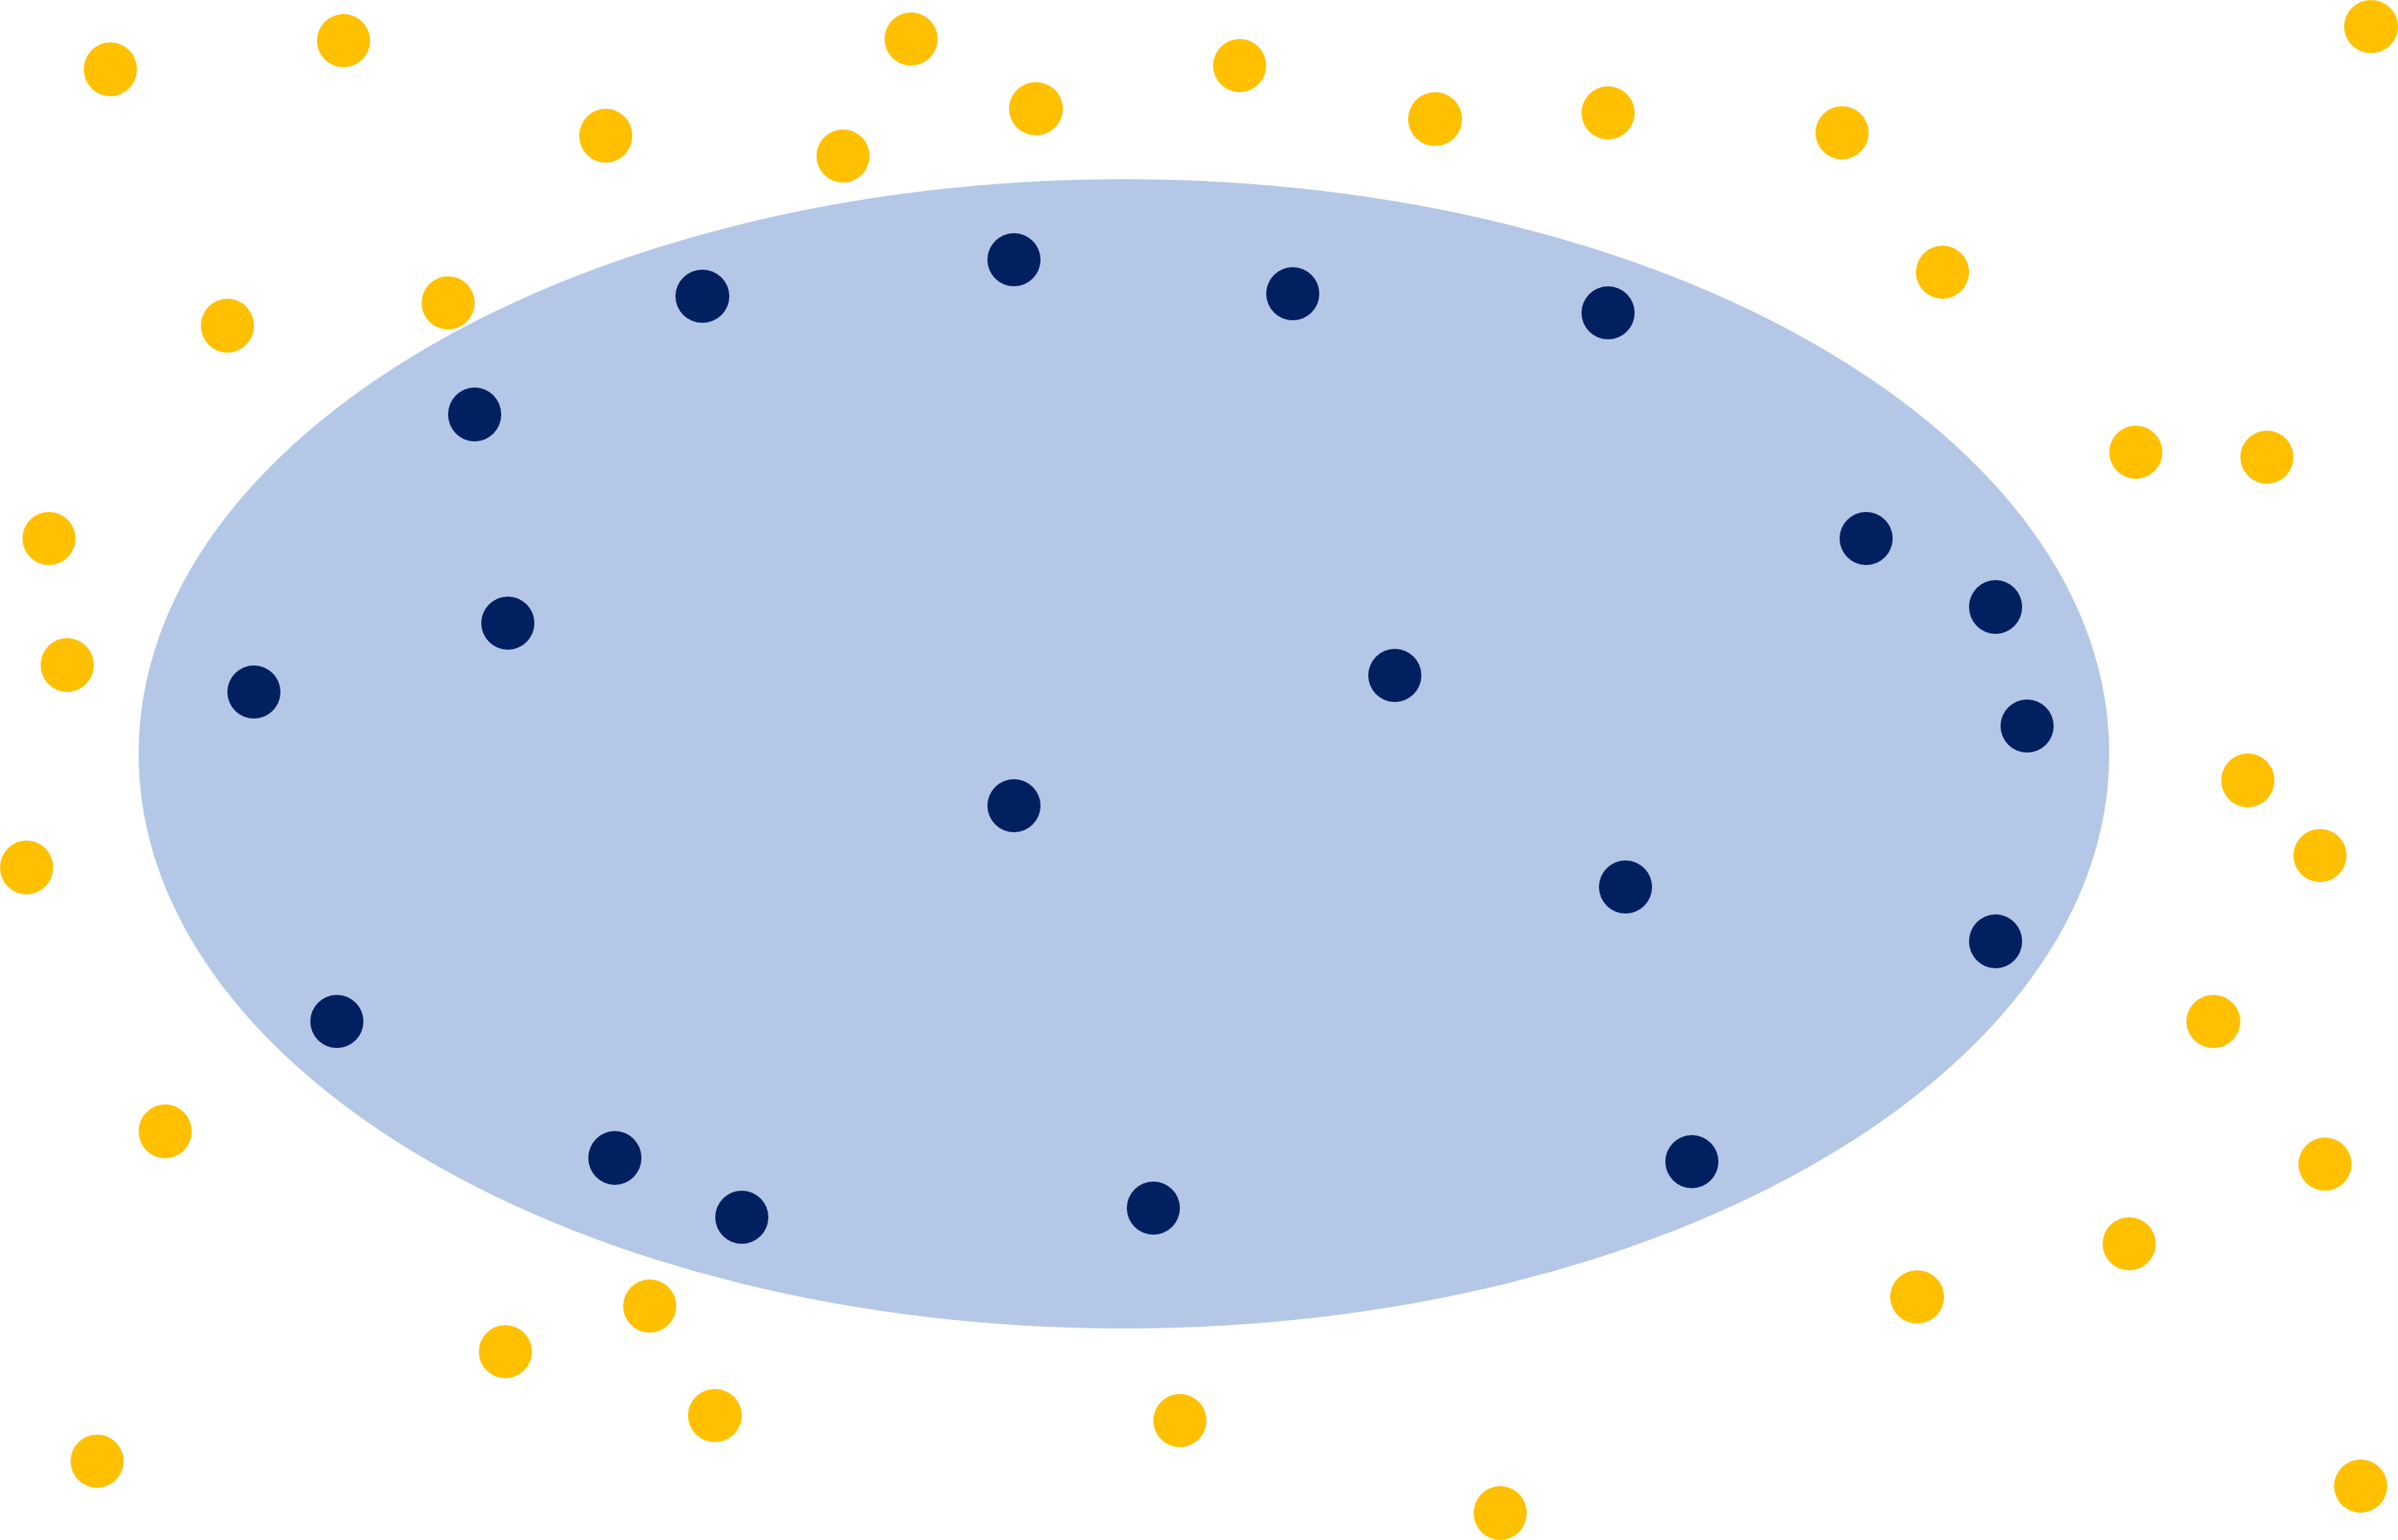
\includegraphics[width=\textwidth]{S4-Explicabilite_globale/figures/filtre2.png}
      \caption{ Les points qui ne sont pas des vecteurs supports sont supprimés.} \label{fig:filtre2}
  \end{subfigure}

    \begin{subfigure}[t]{0.45\textwidth}
      \centering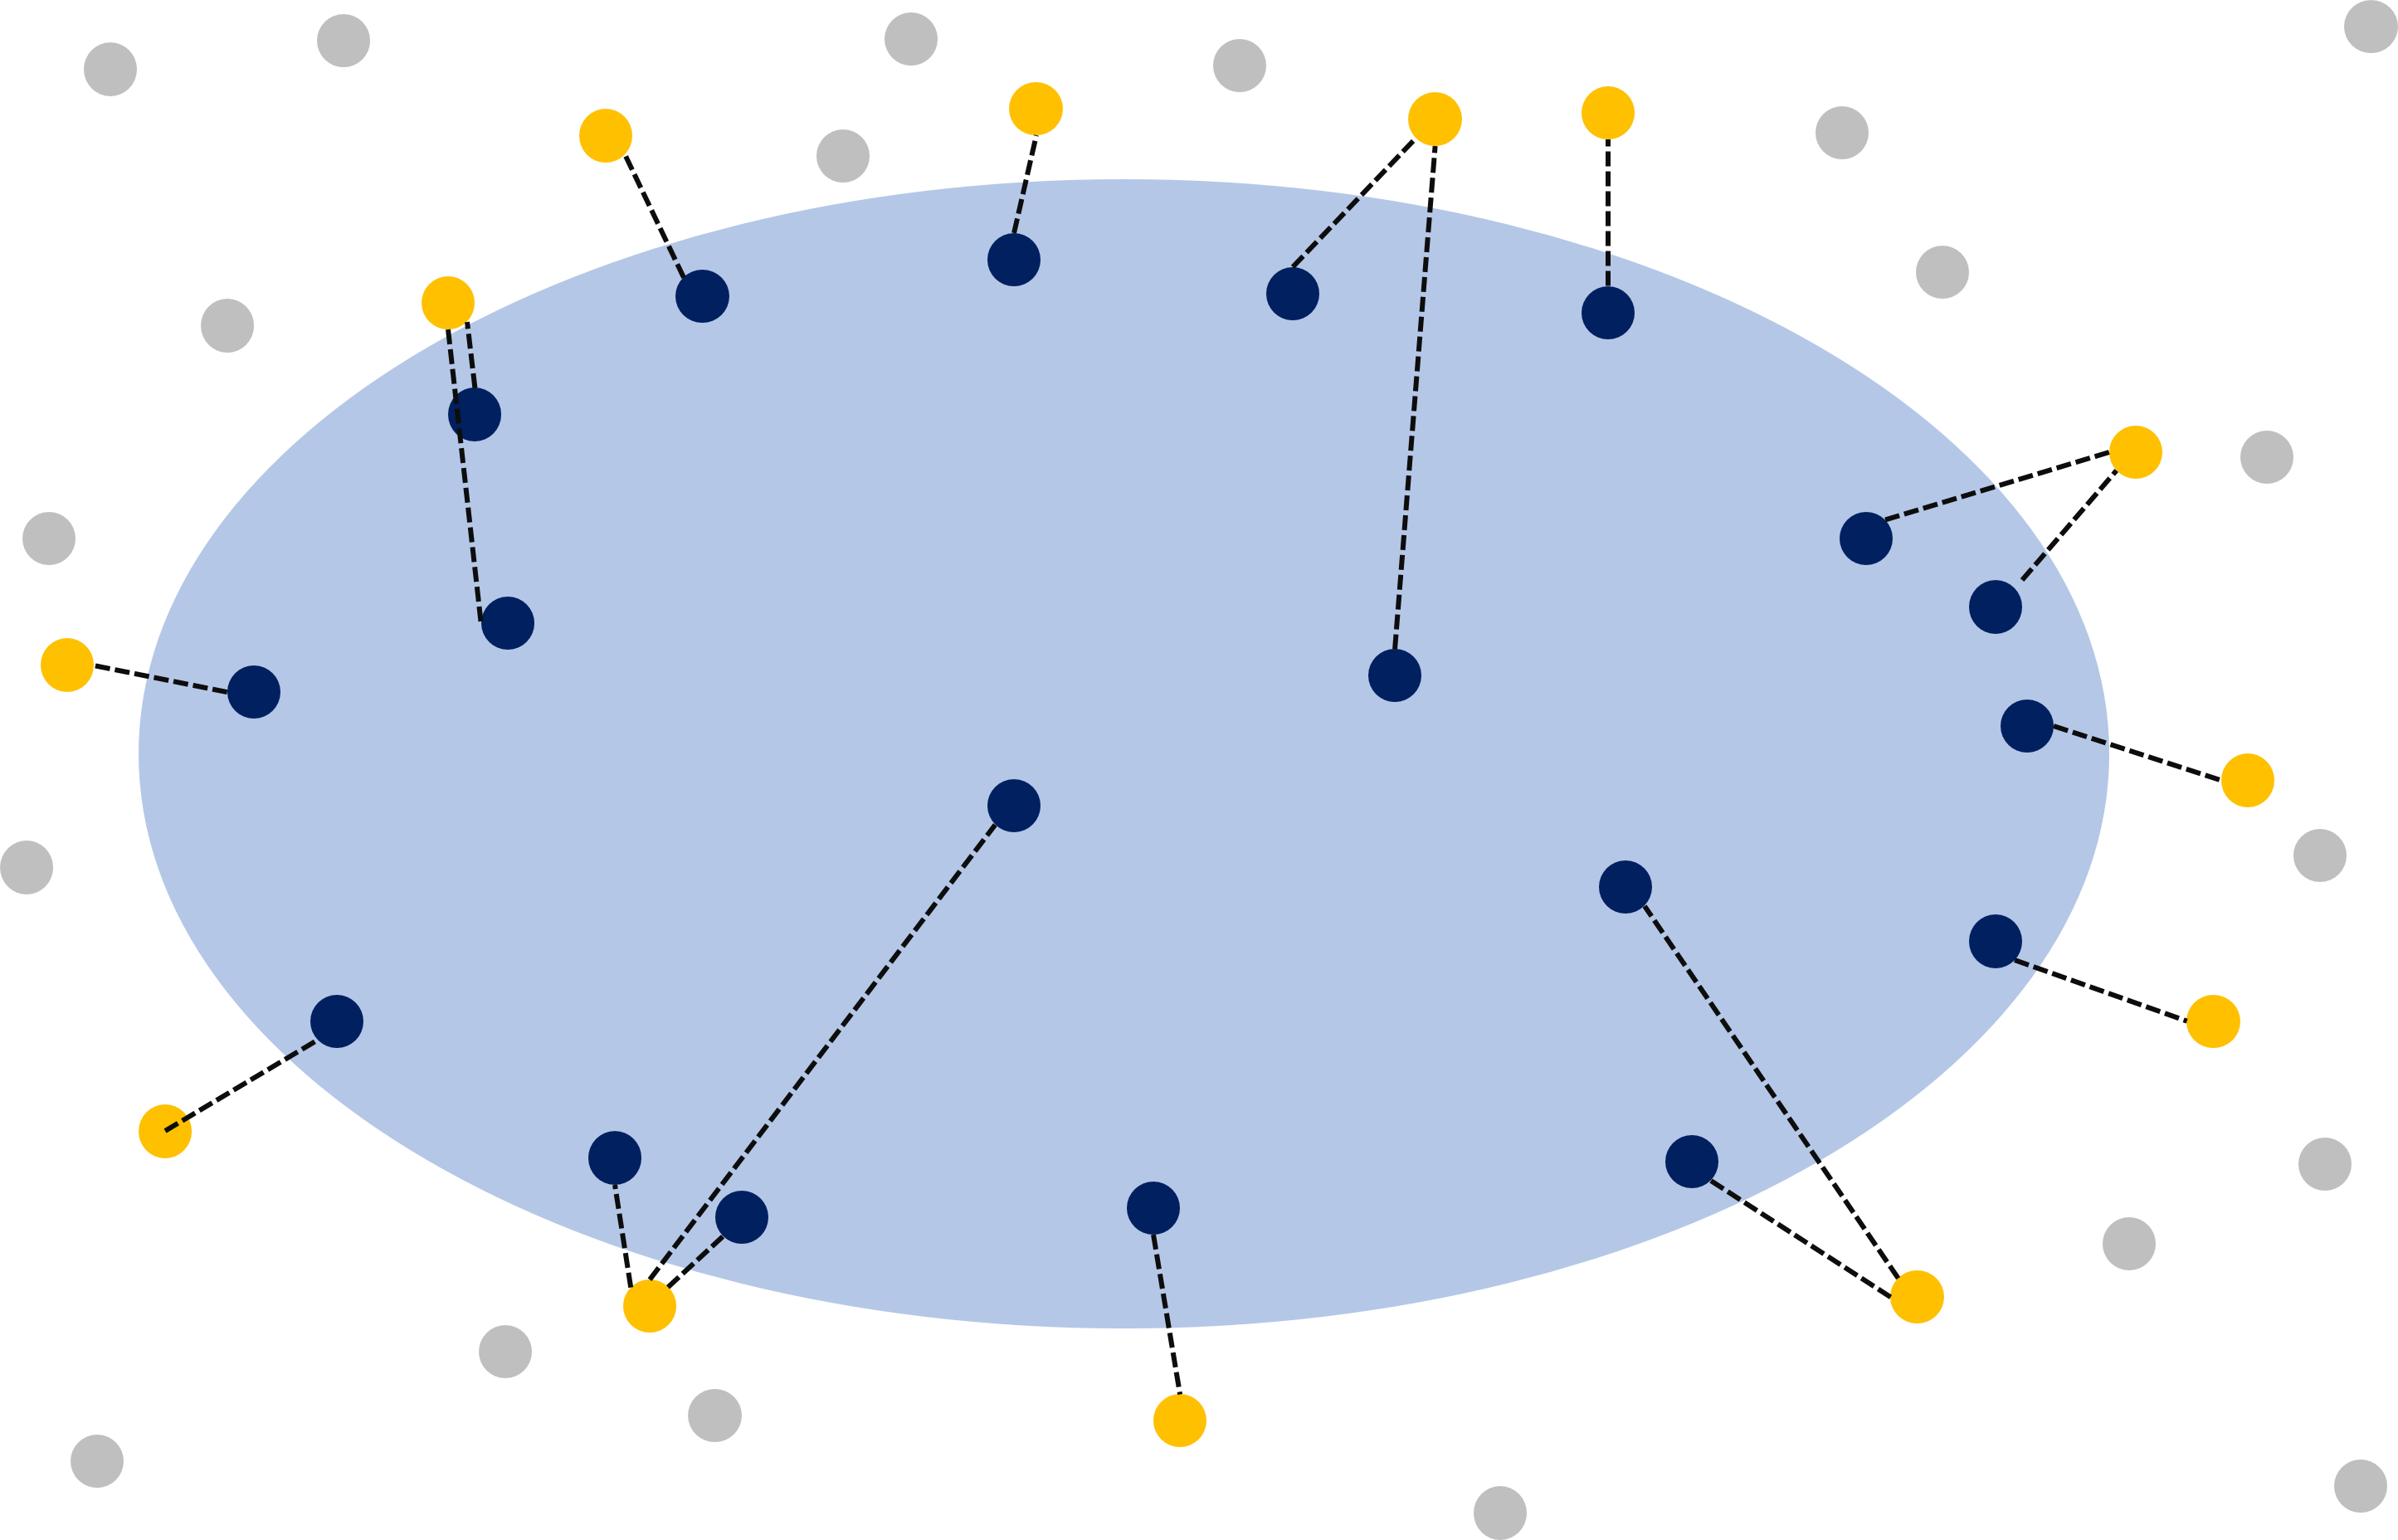
\includegraphics[width=\textwidth]{S4-Explicabilite_globale/figures/filtre3.png}
      \caption{Chaque vecteur support protagoniste est apparié au vecteur support antagoniste le plus proche. Les vecteurs supports antagonistes non appariés sont grisés.} \label{fig:filtre3}
    \end{subfigure} \qquad
    \begin{subfigure}[t]{0.45\textwidth}
      \centering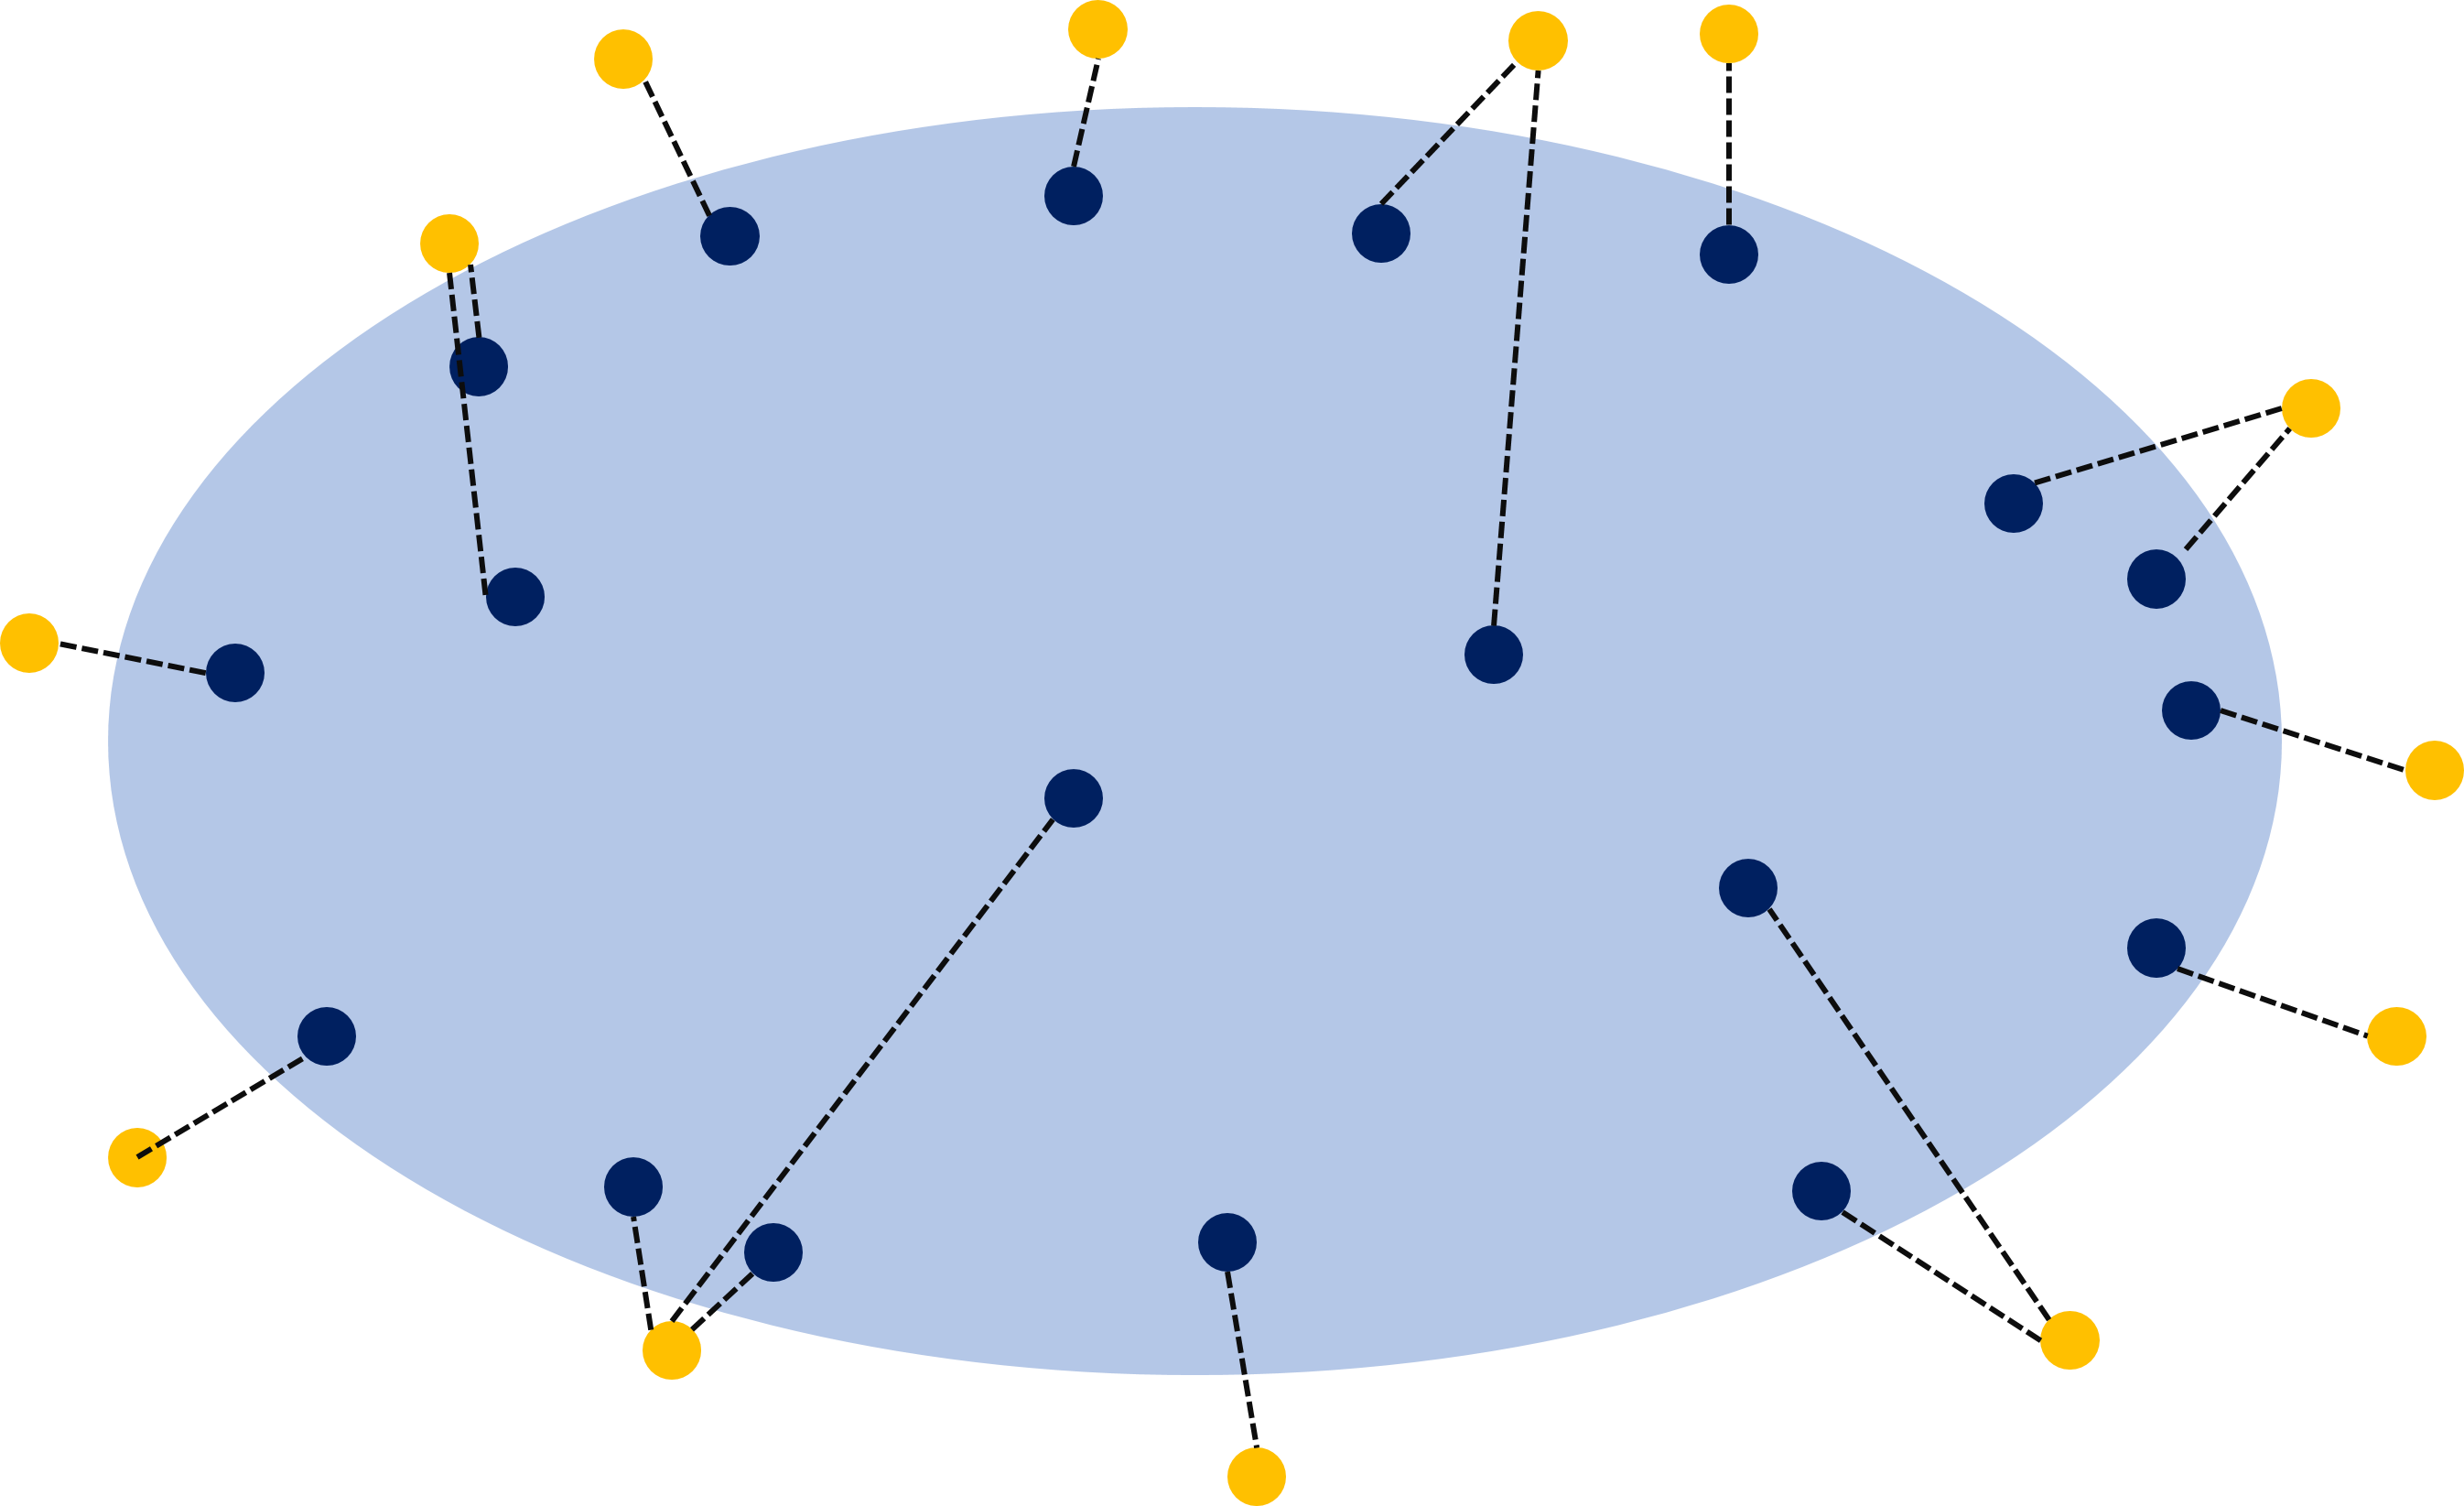
\includegraphics[width=\textwidth]{S4-Explicabilite_globale/figures/filtre4.png}
      \caption{Seuls les vecteurs supports appariés sont conservés.} \label{fig:filtre4}
    \end{subfigure}

\caption{Illustration des principes des différentes étapes de filtre. L'ellipse bleue correspond aux éléments d'une classe observée. Les points bleus appartiennent à la classe considérée, ce sont des éléments protagonistes. Les points jaunes appartiennent aux autres classes, ils sont antagonistes. Les points gris sont ceux supprimés à chaque étape. } \label{fig:filtre}
\end{figure}

Les deux dernières étapes sont illustrées dans la figure~\ref{fig:filtre}. La suppression des doublons consiste à ne conserver qu'un seul point au cas où plusieurs seraient au même endroit, et n'est donc pas visible sur cette illustration.
Dans le contexte One \textit{vs.} Rest, les points de la classe étudiée sont situés à l'intérieur de l'ellipse bleue. Les points en dehors de cette ellipse peuvent être de toutes les autres classes.
Les sous figures~\ref{fig:filtre1} et~\ref{fig:filtre2} montrent le filtre sur les vecteurs supports. Les points grisés en figure~\ref{fig:filtre1}  sont les points candidats qui ne sont pas des vecteurs supports.
% TODO Harold : je ne mettrai pas de gris, mais tous les points soit bleu soit gris. avec une frontière différente (pointillée) pour montrer les frontières du MO. ensuite en b on a le svm avec ses frontières et ses SV.
La figure~\ref{fig:filtre2} présente le même espace avec ces points de données en gris supprimés.
La figure~\ref{fig:filtre3} montre l'appairage entre chaque vecteur support protagoniste et le vecteur support antagoniste le plus proche. Un vecteur support antagoniste peut ainsi être apparié à plusieurs vecteurs supports protagonistes. Cette étape permet de conserver \textit{au maximum} $2*P$ vecteurs supports, avec $P$ le nombre de vecteurs supports protagonistes.
Pour appliquer ce filtre, il faut dans un premier temps entraîner un SVM.
% Approche SVM

\paragraph{Entraînement du SVM}
Avec le SVM entraîné, nous nous concentrons sur les vecteurs supports. Les vecteurs supports sont des points de données intéressants utilisés par le SVM pour apprendre sa fonction de décision.

%  Tout d'abord, comprenons mieux les informations que nous voulons extraire.
%
% \begin{figure}[h!tpb]
%  \centering 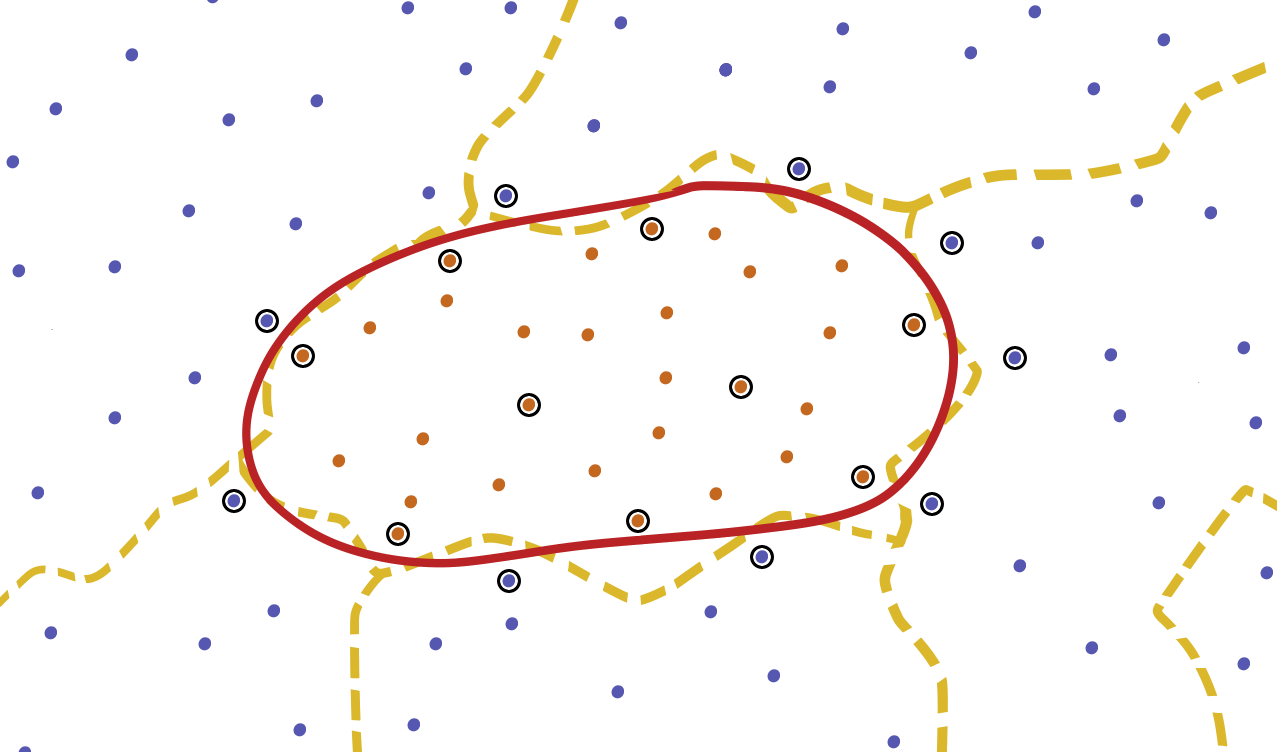
\includegraphics[width=0.8\textwidth]{S4-Explicabilite_globale/figures/svm_frontiere.png}
% \caption{Classification entre une classe A (points orange) et les autres (points bleus). La frontière de décision exacte du modèle original, en pointillés jaunes, n'est pas tangible. La frontière rouge représente l'hyperplan du SVM pour la classe A. Les vecteurs supports délimitant cet hyperplan sont entourés en noir. } \label{fig:svm_decision_boundaries}
% \end{figure}
%
% La Fig.~\ref{fig:svm_decision_boundaries} montre comment obtenir une meilleure idée d'une frontière de décision approximative, en visualisant les vecteurs supports du SVM. Toutes les lignes pointillées jaunes illustrent la représentation mentale de l'utilisateur des limites de décision du MO.
%
% Les points orange et bleus représentent respectivement les instances d'une classe étudiée A et les instances de toutes les autres classes. Tous les points encerclés en noir sont les vecteurs supports du SVM. Ils aident à déterminer la limite de décision du SVM pour cette classe A, représentée dans la Fig.\ref{fig:svm_decision_boundaries} par une ligne rouge.

% Cette frontière est rendue compréhensible pour les humains en observant des exemples intéressants caractérisant la décision du MO.
% Le coût de la précision pour obtenir cette explicabilité est supporté par le SVM et non par la MO.

La figure~\ref{fig:model_architecture} compare les architectures du MO, sur la première ligne et du SVM sur la seconde. Pour un MO donné, l'architecture des premières couches est conservée, et devient la vectorisation en seconde ligne. La classification est effectuée par un SVM à noyau gaussien. Pour que le SVM copie le MO, il doit être entraîné sur les décisions de classification du MO. L'entrée du MO correspond aux données réelles $(X,Y)$, $X$ étant les données vectorisées et $Y$ étant la classe. Il produit en sortie une décision $\bar{Y}$. L'entraînement du SVM prend la même entrée $X$, mais la cible est $(\bar{Y})$ : il est entraîné dans les résultats de classification du MO. Le jeu de données d'entraînement est le même ou à défaut un sous-ensemble.

\begin{figure}[h!tpb]
\centering 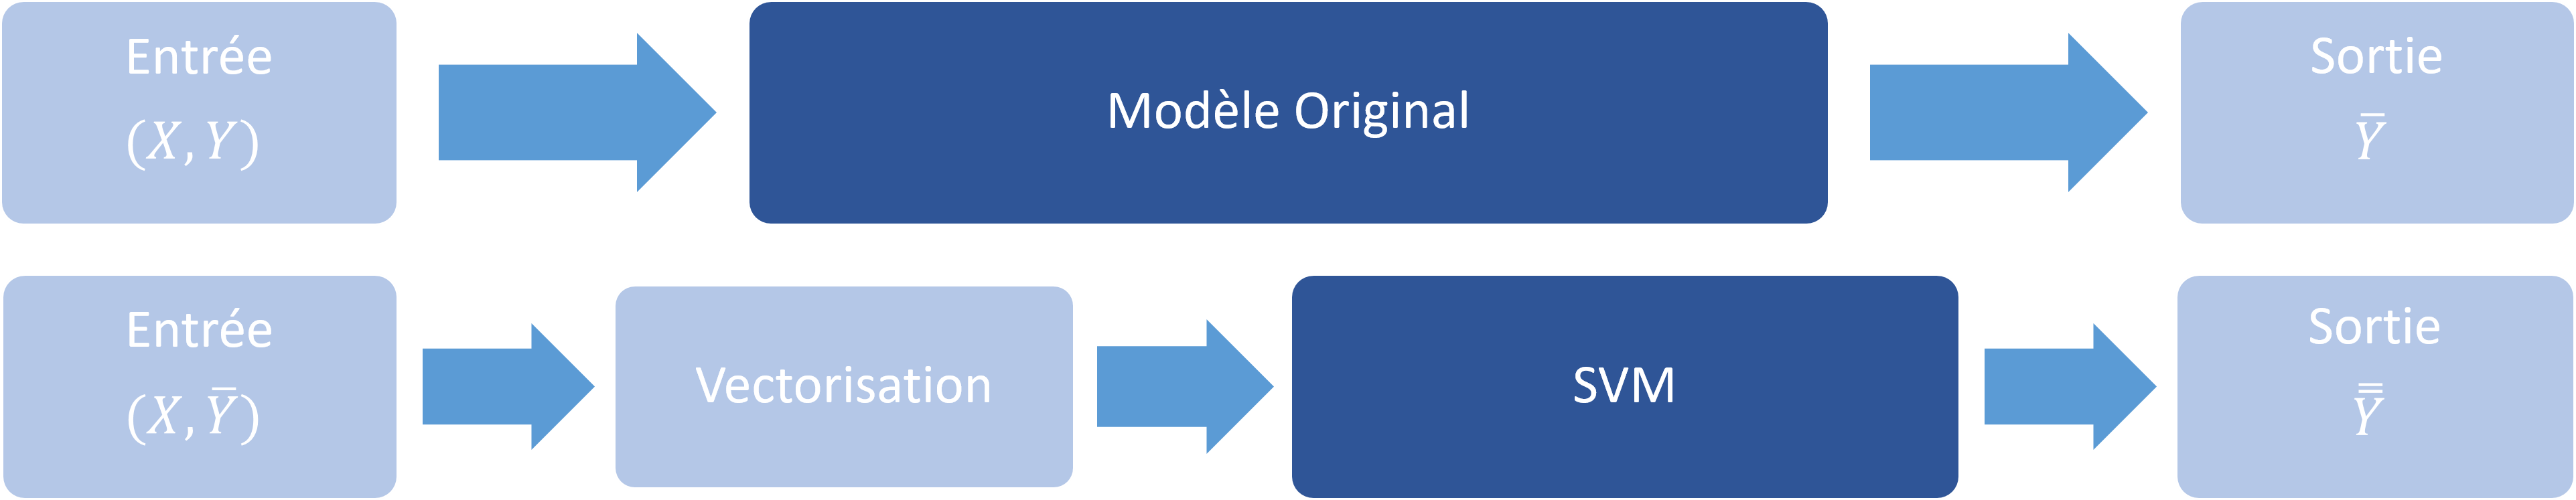
\includegraphics[width=\textwidth]{S4-Explicabilite_globale/figures/model_architecture.png}
\caption{Comparaison entre le modèle boîte noire et les architectures SVM. L'entrée du SVM est basée sur la sortie du modèle original.} \label{fig:model_architecture}
\end{figure}

Les vecteurs supports du SVM ainsi déterminés sont appariés par classe, un vecteur positif avec son vecteur négatif le plus proche. Cette liaison donne des couples pertinents d'exemples factuels et contre-exemples pour une classe donnée.

\paragraph{Les vecteurs support}
Le SVM est composé de $n-1$ classifieurs One \textit{vs.} Rest. Chacun de ces classifieurs est une fonction de décision, basée sur des vecteurs supports $SV$. Son signe de sortie correspond à une classe (positif) ou au reste (négatif). La fonction de décision pour une instance $x$ est :

\begin{equation}
\sum_{i \in SV}y_i\alpha_i K(x_i,x)+b
\end{equation}

Avec $K$ la fonction noyau gaussienne :

\begin{equation}
   K(x_i, x) = e^{-\gamma||x_i-x||}
\end{equation}

Les coefficients duaux des vecteurs supports $y_i\alpha_i $ sont définis avec leur signe $y \in \{-1,1\}$ et leur valeur $\alpha \geq 0$. Ils peuvent être positifs (protagonistes) : pour une classe, le label du vecteur support est le même. Ils peuvent aussi être négatifs : leur étiquette diffère de la classe donnée.

Un classifieur peut, selon le cas d'utilisation, avoir de nombreux vecteurs supports, en particulier avec des coefficients $y$ négatifs. En associant à chaque vecteur positif le vecteur négatif le plus proche, nous éliminons les vecteurs négatifs non associés. Dans le cadre de l'analyse de textes, nous utilisons la distance cosinus.

Pour fournir une vision claire à l'utilisateur, il est nécessaire de trier les points les plus pertinents parmi les vecteurs supports, qui sont déjà les points les plus pertinents du jeu de données d'apprentissage.

\subsection{Tri} \label{C4:tri}

Le tri proposé permet de fournir un résumé digeste pour un humain. L'objectif est donc de ressortir un ensemble de moins d'une dizaine de couples d'exemples. Il est possible de laisser la main à l'utilisateur ou utilisatrice, afin de lui laisser choisir le niveau de zoom qu'iel souhaite.

% SVM
Encore une fois, de nombreuses techniques sont à notre disposition. Il est possible de se baser sur le SVM et trier les couples de vecteurs par somme de leurs valeurs alpha. Il est également possible de prendre un point de la classe étudiée (exemple) au hasard, et effectuer une approximation polygonale en passant par une heuristique gloutonne de sélection du point le plus éloigné du point précédent, ou du barycentre des points sélectionnés.

% CAH
Nous proposons de regrouper les exemples négatifs, en un nombre réduit de groupes. Nous discuterons dans la suite d’une méthode permettant de calculer de tels groupes. Pour chaque groupe constitué, un seul élément est conservé. Ce mécanisme permet d'assurer une bonne répartition des exemples et contre-exemples sélectionnés.

\begin{figure}[h!tpb]
    % \begin{subfigure}{1\textwidth}
    %   \centering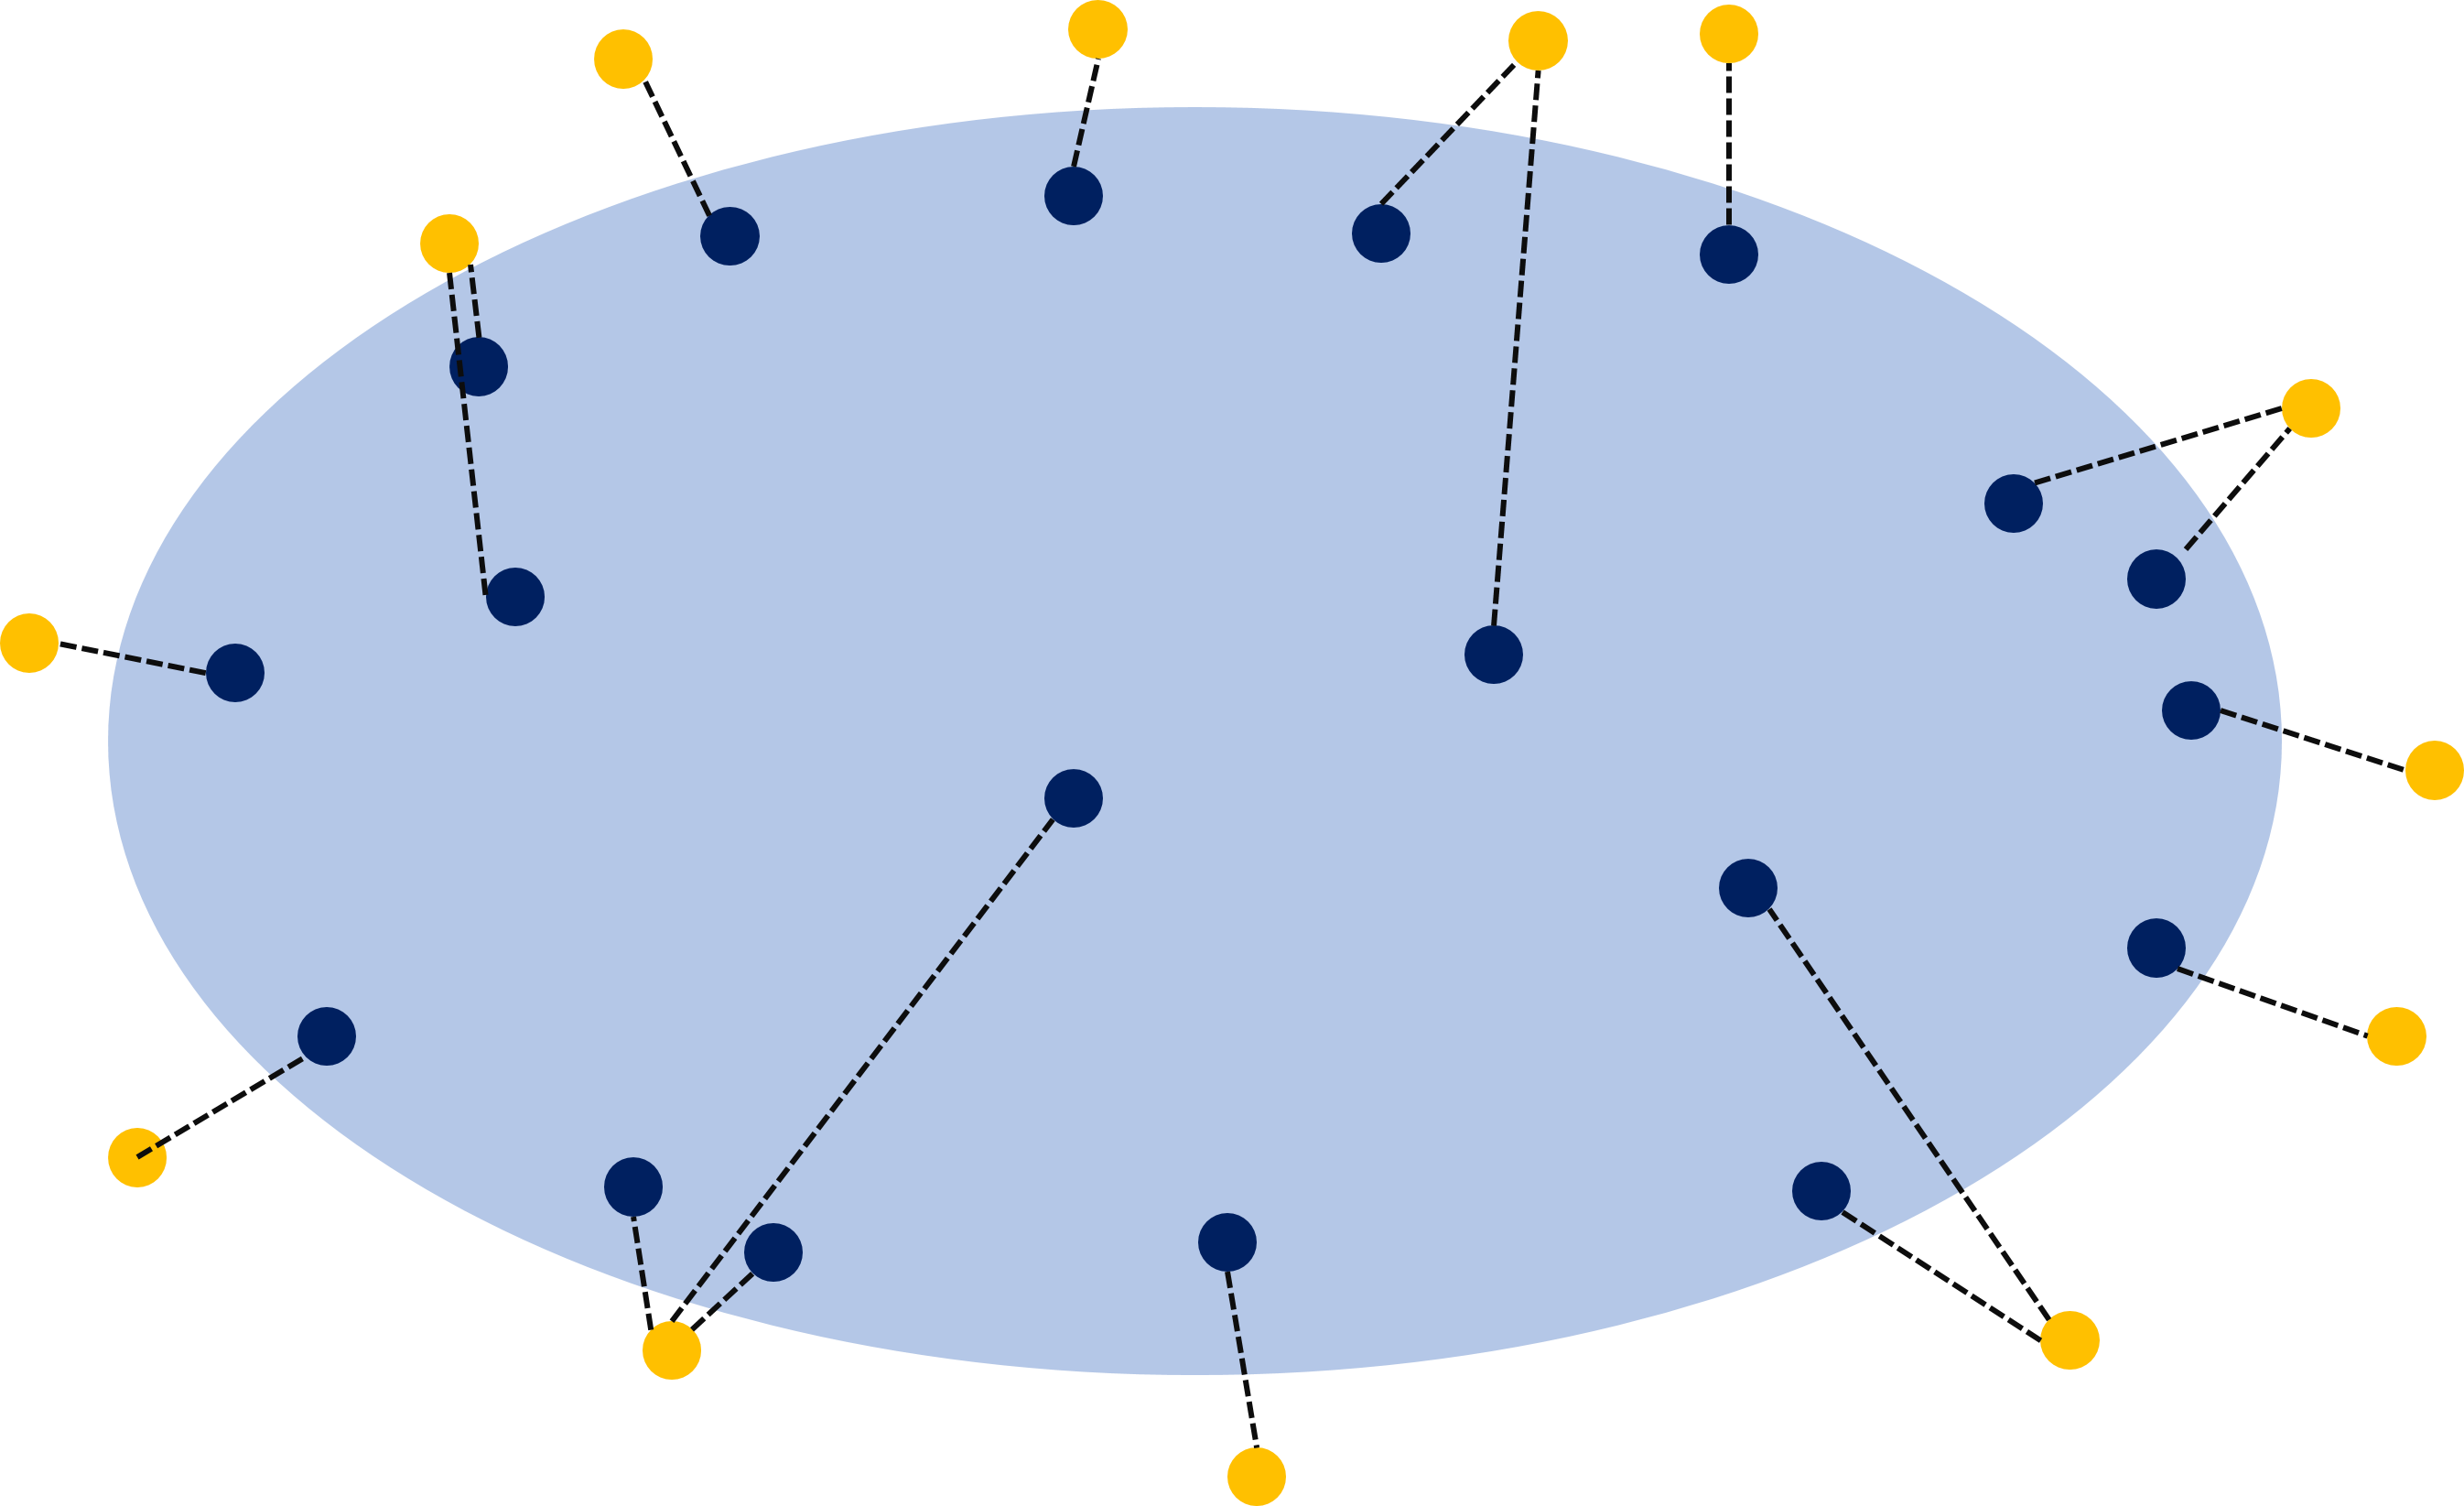
\includegraphics[width=0.5\textwidth]{S4-Explicabilite_globale/figures/filtre4.png}
    %   \caption{[Optionnel] Ensemble des vecteurs supports protagonistes et antagonistes de la classe analysée, représentés avec leurs appairages.} \label{fig:tri0}
    % \end{subfigure}
    \begin{subfigure}[t]{0.45\textwidth}
      \centering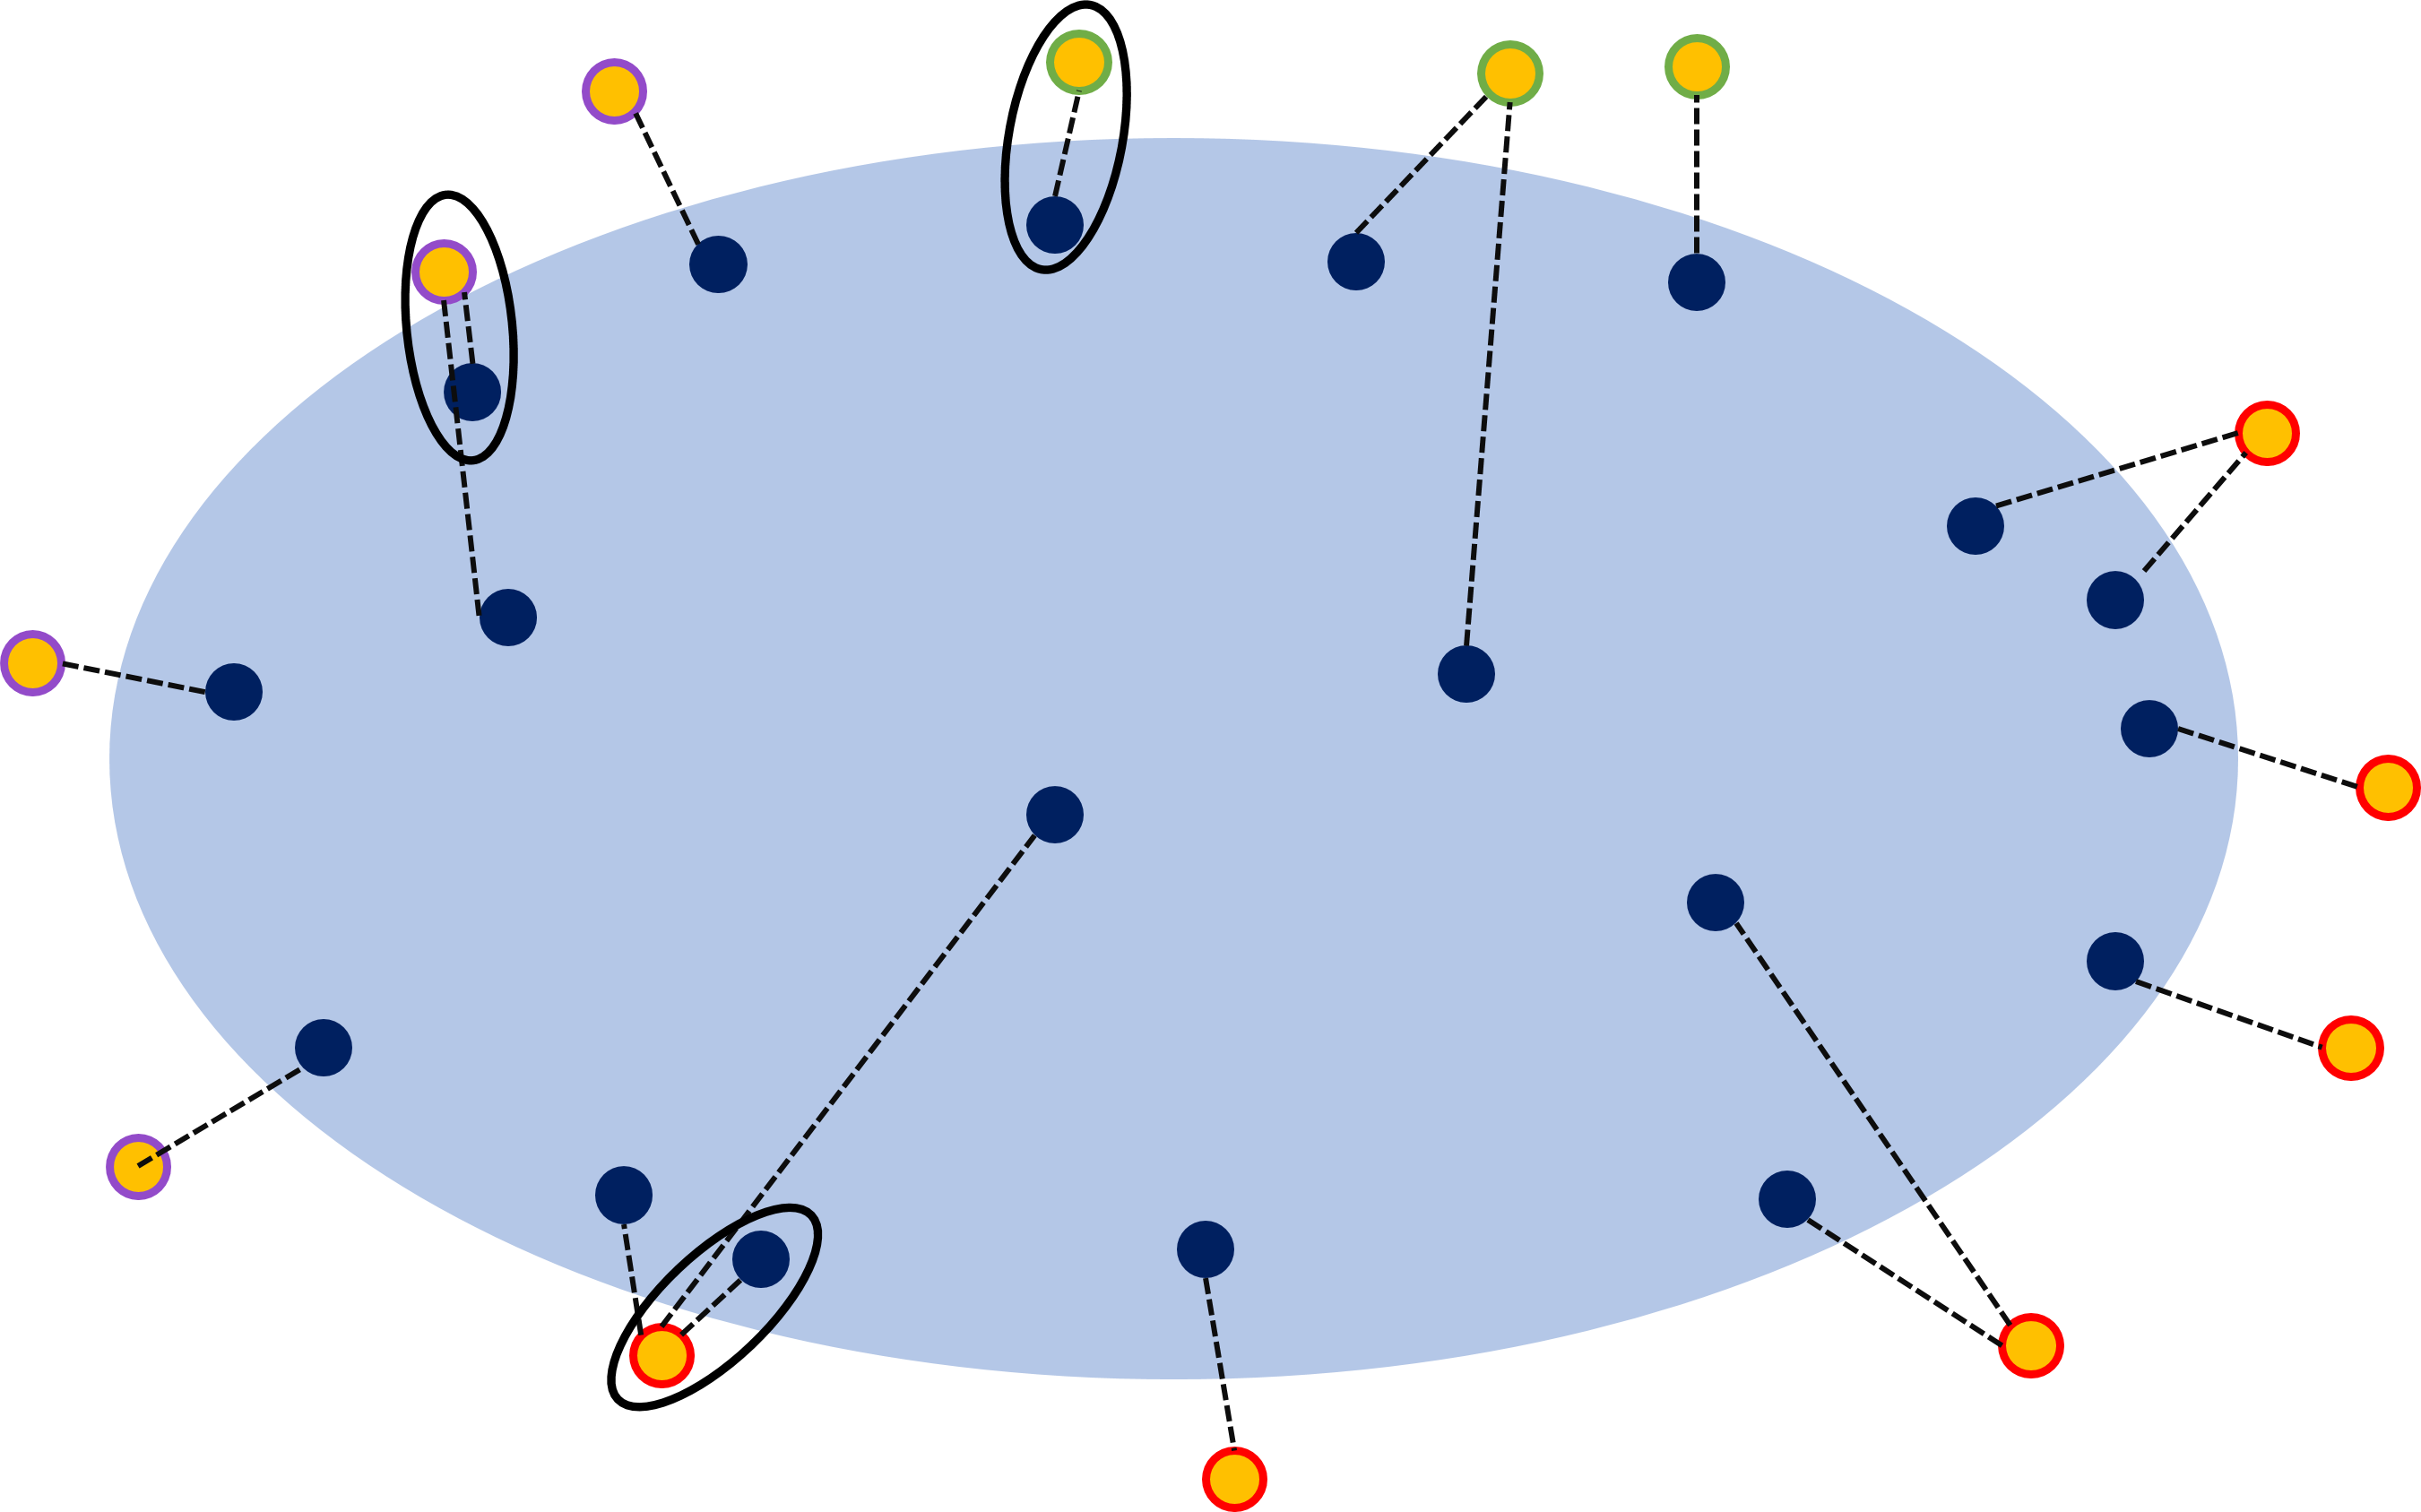
\includegraphics[width=\textwidth]{S4-Explicabilite_globale/figures/tri1.png}
      \caption{Regroupement des vecteurs supports antagonistes en 3 groupes par une méthode quelconque: violet, vert et rouge. Pour chaque groupe, la paire de distance minimale est entourée.} \label{fig:tri1}
    \end{subfigure} \qquad
    \begin{subfigure}[t]{0.45\textwidth}
      \centering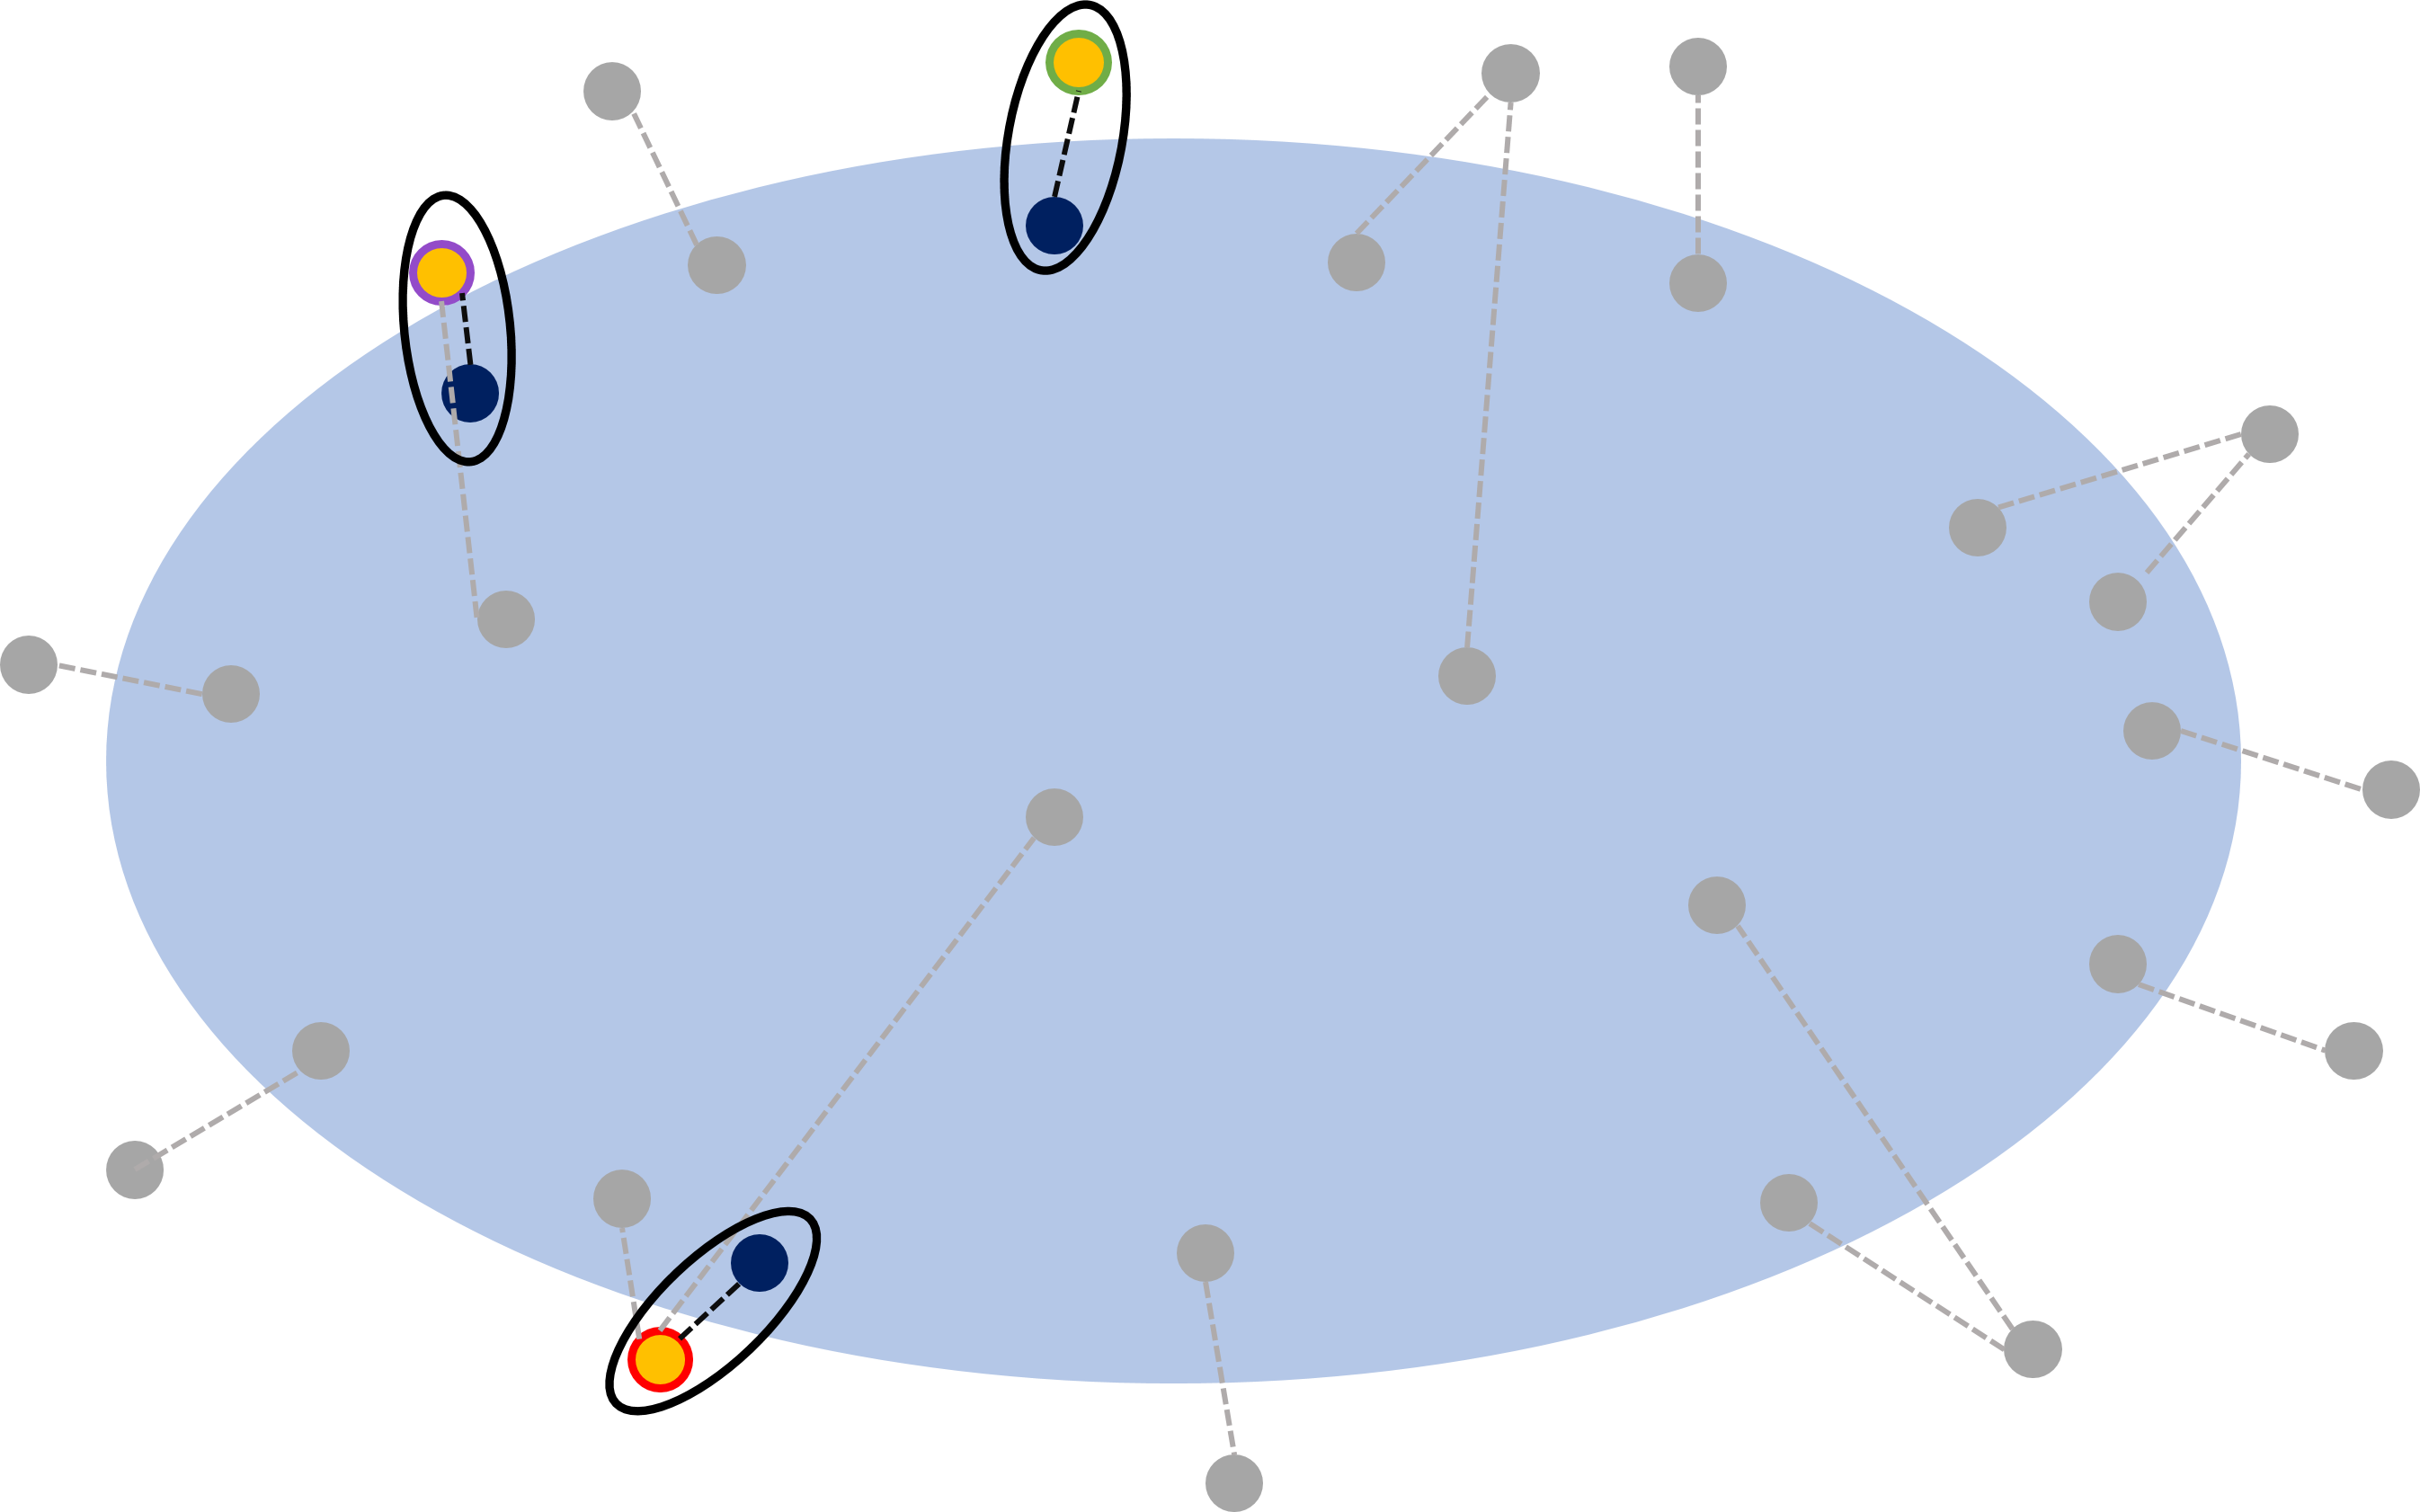
\includegraphics[width=\textwidth]{S4-Explicabilite_globale/figures/tri2.png}
      \caption{Seules les paires entourées sont conservées, les autres points sont mis de côté.} \label{fig:tri2}
    \end{subfigure}

    \begin{subfigure}[t]{0.45\textwidth}
      \centering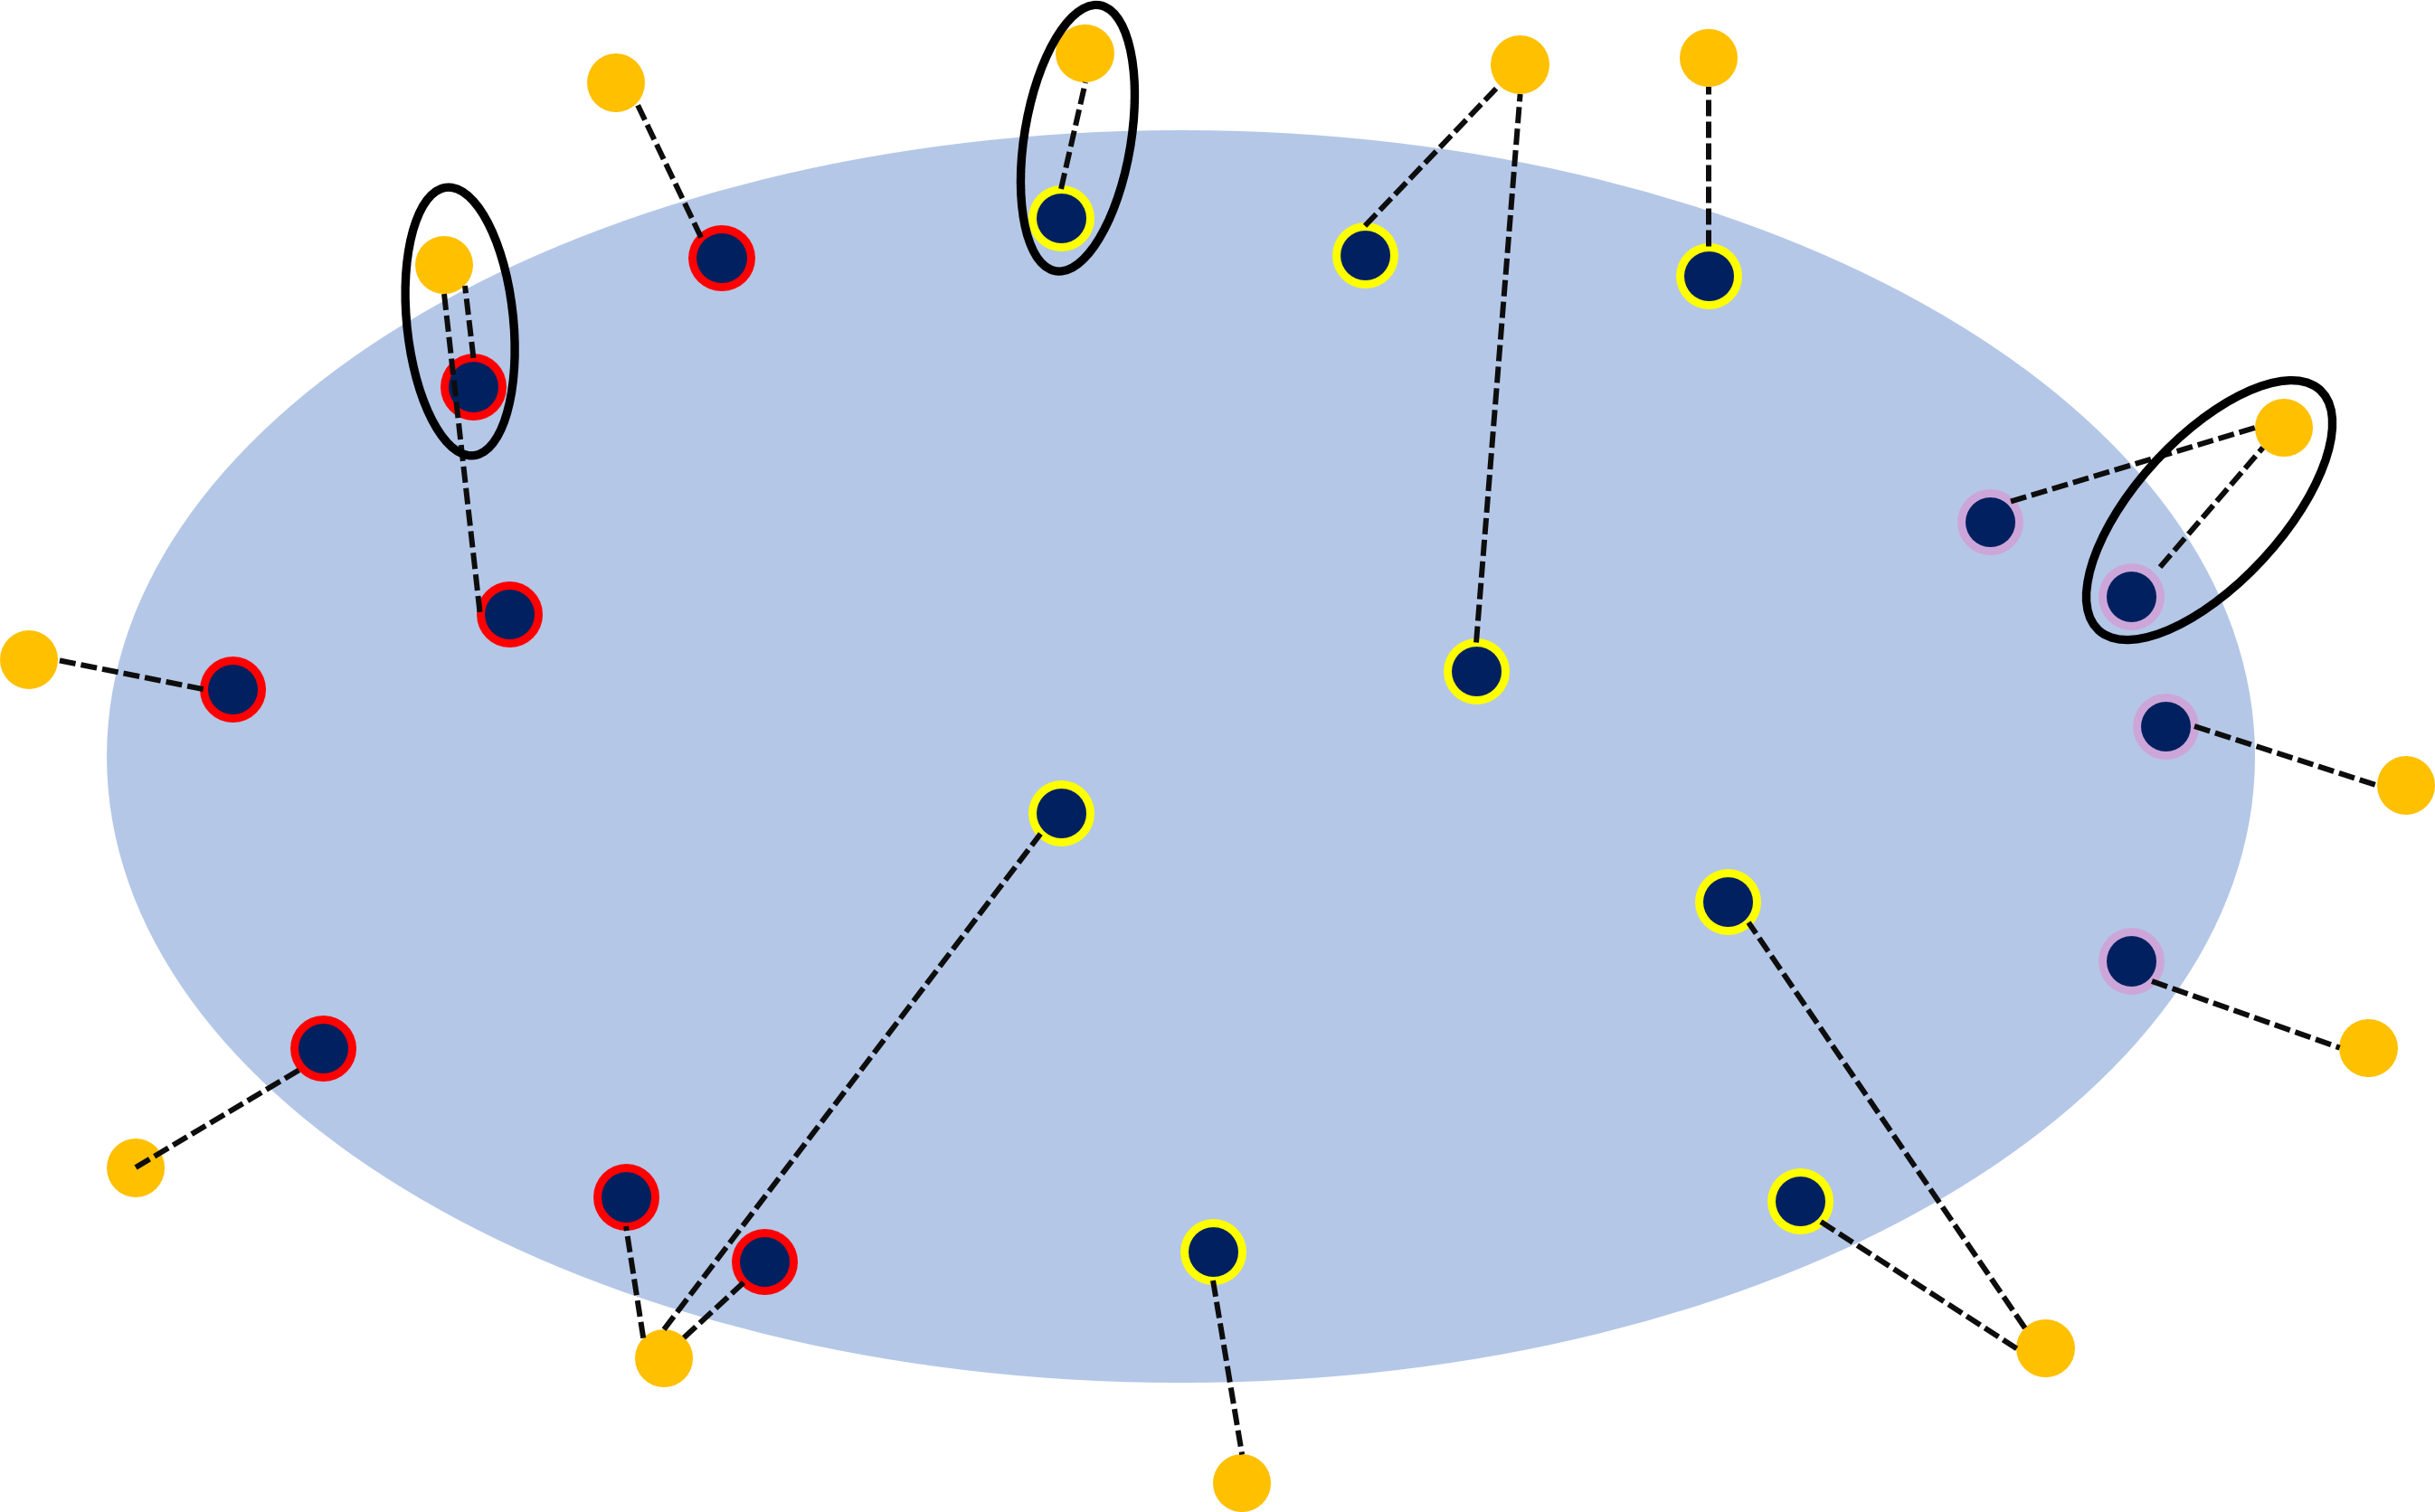
\includegraphics[width=\textwidth]{S4-Explicabilite_globale/figures/tri3.png}
      \caption{Regroupement des vecteurs supports protagonistes en 3 groupes par une méthode quelconque: violet, jaune et rouge. Pour chaque groupe, la paire de distance minimale est entourée.}
      \label{fig:tri3}
    \end{subfigure} \qquad
    \begin{subfigure}[t]{0.45\textwidth}
      \centering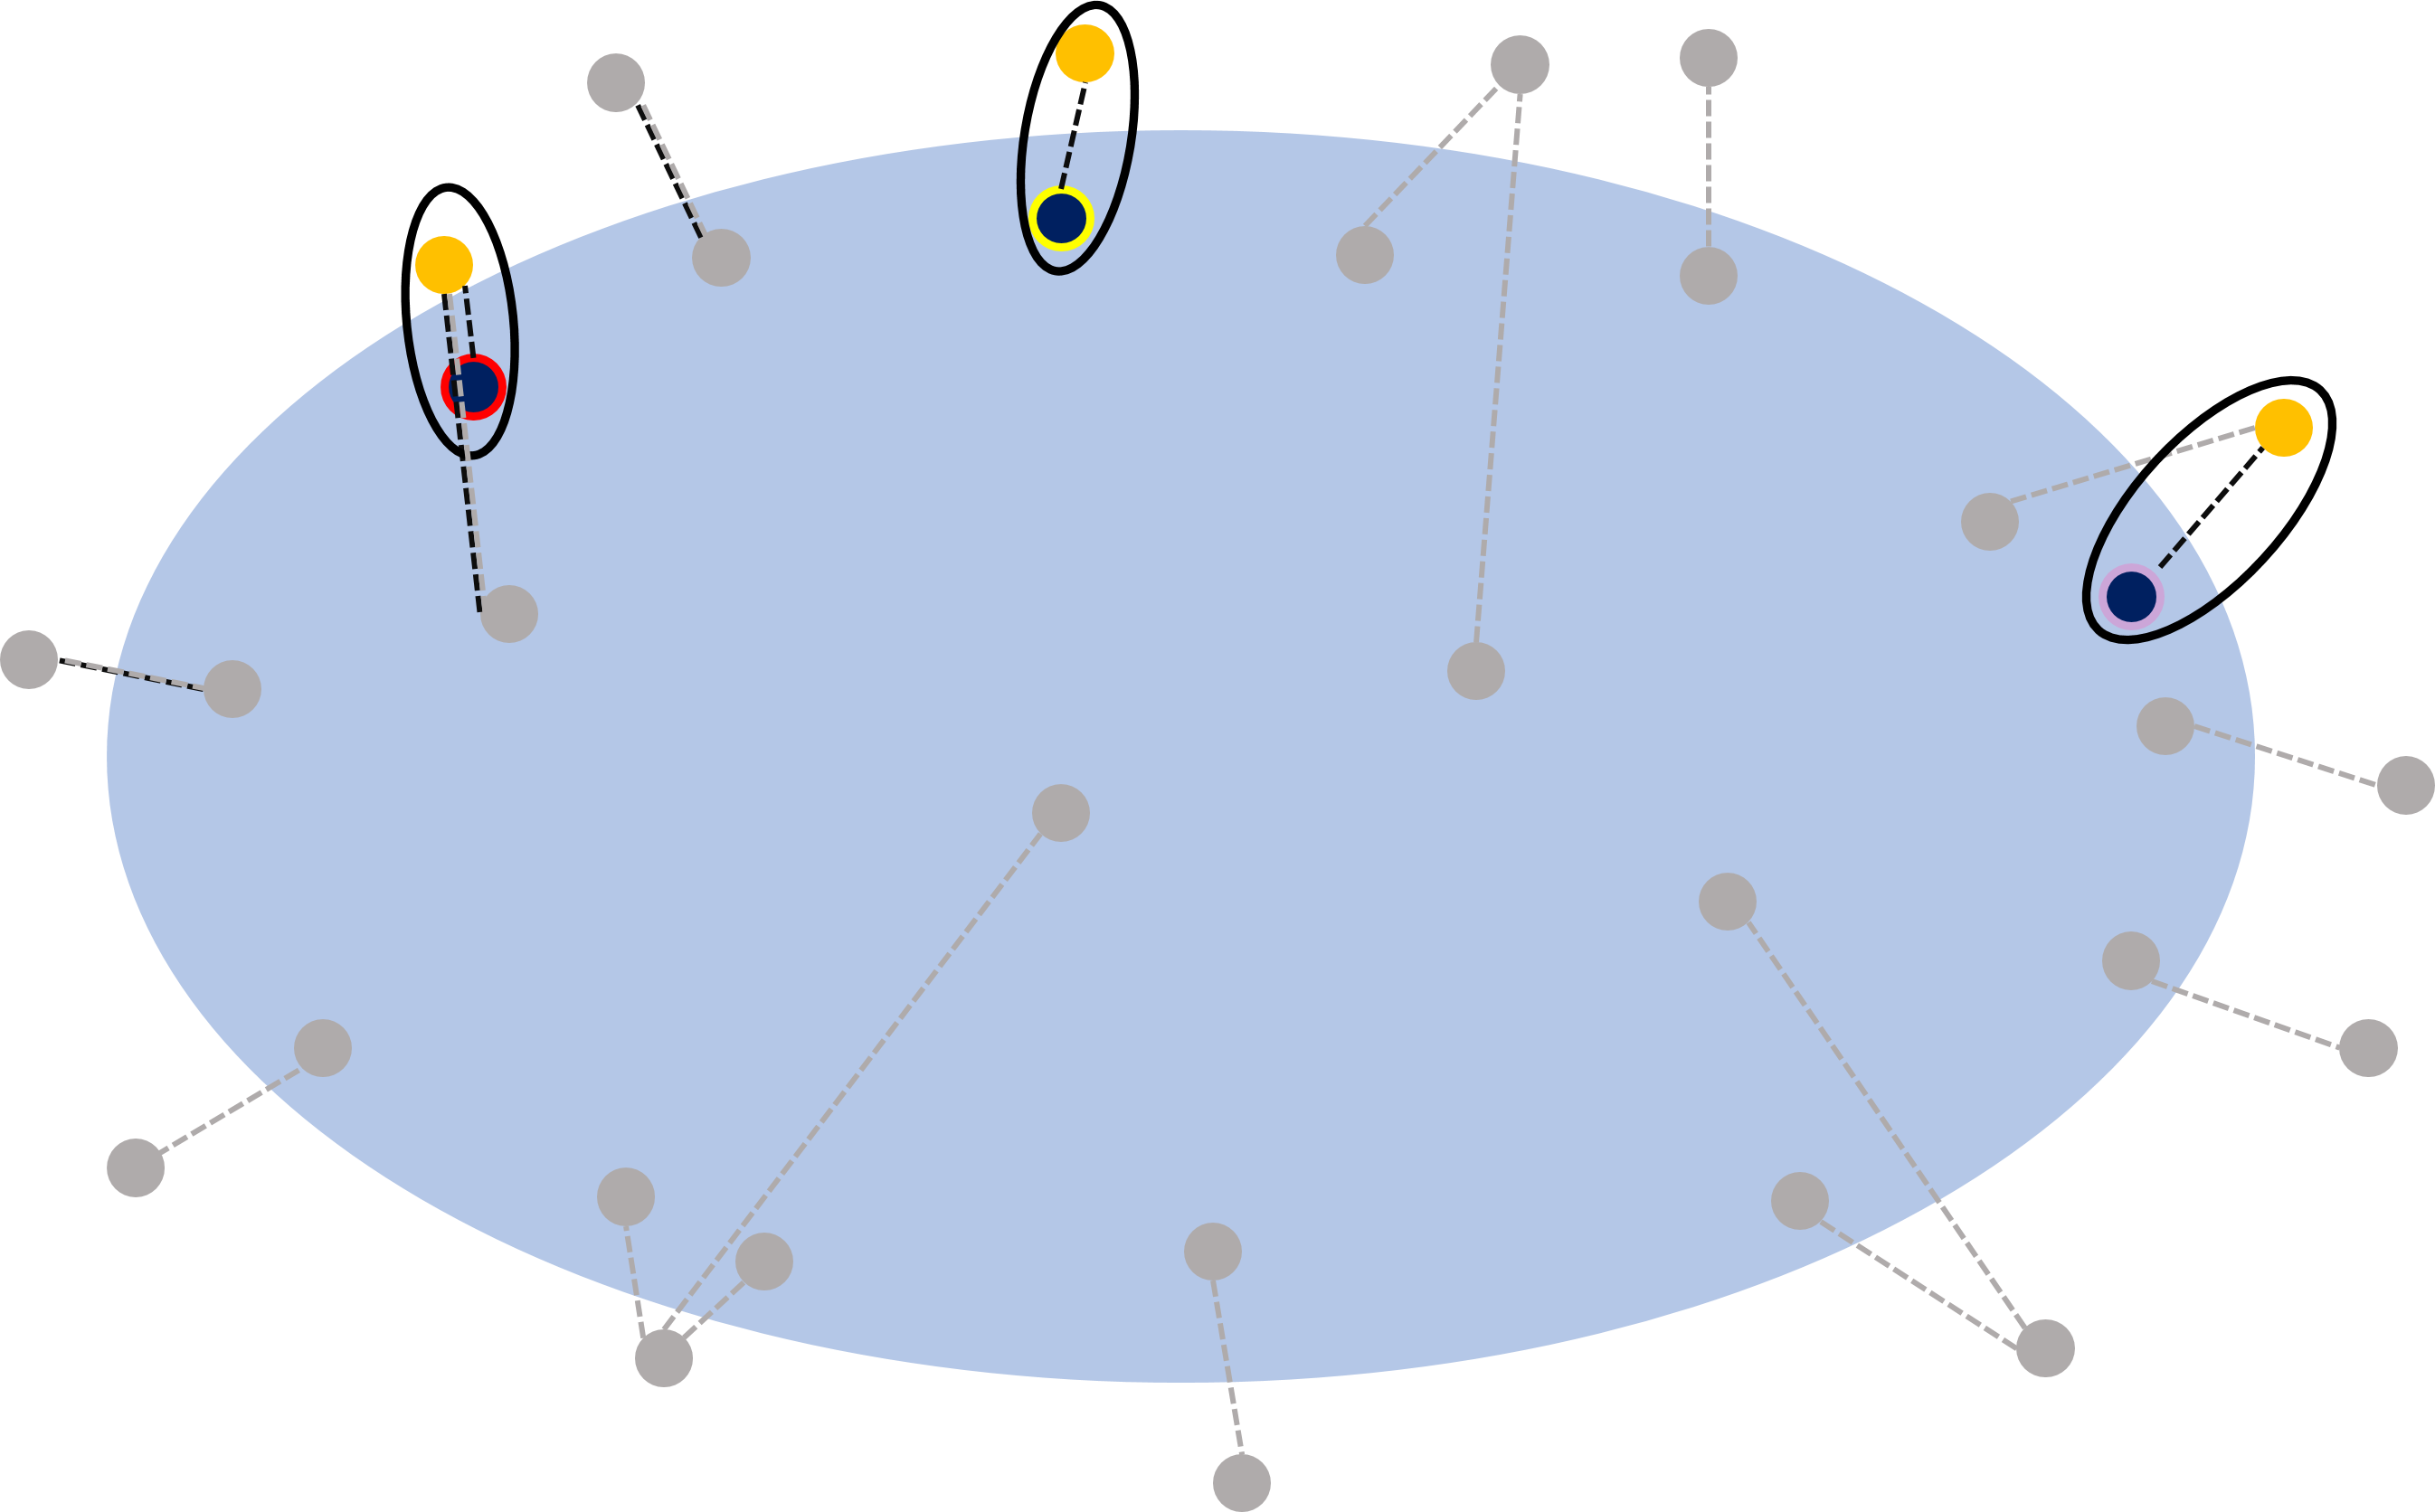
\includegraphics[width=\textwidth]{S4-Explicabilite_globale/figures/tri4.png}
      \caption{Seules les paires entourées sont conservées, les autres points sont mis de côté.} \label{fig:tri4}
    \end{subfigure}

    \caption{Illustration des différentes étapes de tri. } \label{fig:tri}
\end{figure}

La figure~\ref{fig:tri} présente le filtre avec la sélection de $n=3$ paires d'exemples et contre-exemples. Les figures~\ref{fig:tri1} et~\ref{fig:tri2} présentent le premier mode du filtre en effectuant les regroupements sur les vecteurs supports antagonistes. Les figures~\ref{fig:tri3} et~\ref{fig:tri4} présentent le second mode du filtre en effectuant les regroupements sur les vecteurs supports protagonistes.
Pour chaque mode, le principe est identique. Les vecteurs supports (protagonistes ou antagonistes) sont regroupés en $n$ groupes. Pour chaque groupe, le couple d'éléments de distance minimale est présenté, c'est à dire les instances les plus proches de la frontière. Tous les autres éléments sont mis de côté.

Il est également possible de concaténer les résultats des deux modes. La sélection des paires de distance intra paire minimale augmente la probabilité que les paires sélectionnées soient identiques entre les deux modes de regroupements. Si $n$ paires sont demandées, le nombre de paires concaténées des deux modes sera alors compris entre $n$ et $2n$.

Le regroupement est effectué par une Classification Ascendante Hiérarchique (CAH) basée sur le critère de Ward.
Une heuristique classique afin de déterminer le nombre de groupes à conserver consiste à observer le dendrogramme présentant les regroupements et la distance interclasses. La meilleure découpe de ce dendrogramme est classiquement celle apportant le plus d'informations, c'est à dire celle où le saut est le plus important. Nous considérons la CAH comme un zoom, et laissons l'utilisateur couper où iel le souhaite. Les couples d'exemples ainsi sélectionnés sont présentés.

Cette méthode permet de présenter un ensemble restreint et représentatif des couples d'exemples et contre-exemples d'intérêt. Il revient alors à l'utilisateur d'effectuer l'analyse des éléments pour la classe étudiée. Ce travail est à faire pour toutes les classes afin d'obtenir une vision globale du modèle.

% Transition
Maintenant que le protocole est défini, il est appliqué à un cas d'utilisation réel, ce qui nous permet de voir ses avantages, ses limites et ses possibilités d'amélioration.

\section{Application} \label{C4:application}

Nous appliquons cette stratégie de caractérisation au cas d'usage LEGO présenté en chapitre~\ref{C3}. Pour rappel, c'est un problème de classification multi-classes, mono-label, par phrase. Il y a 26 classes, l'une d'entre elles comprenant les phrases légales. Cette classe a un intérêt fonctionnel tout particulier : elle correspond à des phrases ``correctes'', là où tous les autres motifs sont des phrases ``incorrectes''.

Le modèle étudié pour cette application est le modèle à attention présenté en chapitre 3. Dans ce chapitre, le modèle à attention est considéré comme une boîte noire. Les données candidates de la section~\ref{C4:candidats} sont les données d'entraînement présentées en chapitre 3. L'implémentation du filtre présentée précédemment est appliquée en section~\ref{C4:app_filtre}. Celle du tri est appliquée en section~\ref{C4:app_tri}.

\subsection{Filtre} \label{C4:app_filtre}

% Caractéristiques de MO
Le SVM entraîné est un SVC de sci-kit learn, avec un noyau gaussien. L'ensemble d'apprentissage est le même que celui utilisé pour le MO, mais la classe à prédire est la décision du MO, comme spécifié dans~\ref{C4:filtre}. Il obtient une précision moyenne de $0,997$, signifiant qu'il parvient à imiter le MO.

Le SVM possède 14840 vecteurs support, correspondant à $3,09\%$ de l'ensemble de données d'apprentissage. Les vecteurs supports correspondent à 12077 vecteurs uniques, soit $2,52\%$ de l'ensemble de données d'apprentissage. Certaines phrases de l'ensemble d'apprentissage sont des doublons, d'où la légère variation. Dans notre analyse, nous avons élagué les doublons en sélectionnant le premier de tous les vecteurs supports correspondant à une phrase donnée.

Pour chaque classe, des vecteurs supports sont sélectionnés, divisés en vecteurs supports positifs et négatifs. Une distance cosinus est calculée entre les deux groupes. Comme nous cherchons à retrouver la proximité sémantique des phrases, nous utilisons la distance cosinus. Un vecteur support positif (resp. négatif) donne un exemple factuel (resp. contrefactuel) pertinent. Chaque exemple factuel pertinent de la classe étudiée est apparié avec l'exemple contrefactuel le plus proche.

\begin{table}
    \caption{Exemples factuels pertinents et leurs exemples contrefactuels pour la classe ``Discrimination : contrat étudiant''. La décision du MO associée au contrefactuel et la distance entre l'exemple factuel et le contrefactuel sont également affichées.} \label{tab:results_student}
    \begin{tabular}{|p{0.32\textwidth}|p{0.5\textwidth}|p{0.13\textwidth}|}
        \hline
        \textbf{Exemple factuel } & \textbf{Exemple contrefactuel associé (CFE)} & \textbf{Distance cosinus} \\ \hline
        Profil recherché : Etudiant(e), salarié(e), retraité(e). & Etudiant(e), retraité(e), travaillant à temps partiel ou en recherche d'emploi, vous êtes avant tout passionné(e) par les enfants ? Devenez un(e) nounou Kangourou ! & $0,066$ \\ \hline
        Etudiants acceptés. & 35 H/Semaine minimum Etudiants acceptés. & $0,050$ \\ \hline
    \end{tabular}
\end{table}

La table~\ref{tab:results_student} présente deux couples d'exemples factuels et contrefactuels pour la classe \textit{``Discrimination : contrat étudiant''}. Il est illégal en France de spécifier que le candidat d'une offre d'emploi doit être un étudiant.

\begin{table}
    \caption{Diminution des paires pour la classe \textit{``Discrimination : Contrat étudiant''}}  \label{tab:combinatoire}
    \begin{tabular}{|p{0.3\textwidth}|p{0.15\textwidth}|p{0.28\textwidth}|p{0.22\textwidth}|}
        \hline
         & \textbf{Légal} & \textbf{Contrat étudiant} & \textbf{Paires} \\ \hline
        Données brutes             & 385754  & 2477 & 955 512 658 \\ \hline
        \multicolumn{4}{|l|}{Suppression des doublons}              \\ \cline{1-4}
        Vecteurs uniques           & 259 853 & 841  & 218 536 373 \\ \hline % facteur 4,4
        \multicolumn{4}{|l|}{Sélection des vecteurs supports}        \\ \hline
        vecteurs supports           & 4 688   & 151  & 707 888     \\ \hline % facteur 309
        \multicolumn{4}{|l|}{Appairage par similarité cosinus}       \\ \hline
        Paires de vecteurs supports & 43      & 151  & 151         \\ \hline % facteur 4 688
    \end{tabular}
\end{table}

Pour cette classe, nous obtenons $151$ couples de vecteurs supports positifs et négatifs. Le tableau~\ref{tab:combinatoire} montre les réductions consécutives du nombre de points  en partant du nombre de données brutes). La dernière colonne présente le nombre de paires possibles. Avant le filtre, le nombre de paires d'exemples et contre-exemples dans les données d'entraînement pour la classe \textit{Discrimination : Contrat étudiant} est proche du milliard. Pour cette classe spécifiquement, la suppression des doublons divise le nombre de paires par $4$ environ. La sélection des vecteurs supports divise par $309$ ce nombre, et l'appairage final le divise par $4 688$.
Cette réduction est notable sur toutes les classes étudiées, et est plus prononcées sur les classes fortement représentées, comme le montre le tableau~\ref{tab:nb_vs}.

\begin{table}
    \caption{Nombre de vecteurs supports protagonistes uniques et de paires d'exemples et contre-exemples obtenus grâce au filtre, par classe. } \label{tab:nb_vs}
    \begin{tabular}{|p{0.65\textwidth}|p{0.15\textwidth}|p{0.1\textwidth}|}
        \hline
            \textbf{Classe}    & \textbf{VS uniques} & \textbf{Paires} \\ \hline
            Discrimination : Activité syndicale ou mutualiste      &     8  &  8      \\ \hline
            Discrimination : Age                                   &  2251  &  579    \\ \hline
            Discrimination : Apparence physique                    &   590  &  311    \\ \hline
            Discrimination : Contrat aidé                          &    15  &  14     \\ \hline
            Discrimination : Contrat étudiant                      &   841  &  151    \\ \hline
            Discrimination : \'Etat de santé                       &  5815  &  1006   \\ \hline
            Discrimination : Grossesse                             &    43  &  30     \\ \hline
            Discrimination : Handicap                              &   674  &  296    \\ \hline
            Discrimination : M\oe urs                              &   102  &  62     \\ \hline
            Discrimination : Nationalité                           &   168  &  123    \\ \hline
            Discrimination : Opinions politiques                   &    27  &  22     \\ \hline
            Discrimination : Origine                               &   349  &  193    \\ \hline
            Discrimination : Résidence                             &  1845  &  369    \\ \hline
            Discrimination : Genre - Au moins un accord au féminin &  1247  &  415    \\ \hline
            Discrimination : Genre - Intitulé exclusivement féminin &  2606  &  478   \\ \hline
            Discrimination : Genre - Mention genre exclusif        &   129  &  84     \\ \hline
            Discrimination : Situsation familiale                  &    29  &  26     \\ \hline
            Discrimination : Taille                                &   173  &  101    \\ \hline
            Droit du travail : Achat de matériel                   &  6018  &  892    \\ \hline
            Droit du travail : CDD Possibilité CDI                 & 12461  &  1154   \\ \hline
            Libertés : Casier Judiciaire                           &   351  &  117    \\ \hline
            Libertés : Tenue vestimentaire                         &    22  &  18     \\ \hline
            Légal                                                  & 259853 &  4688   \\ \hline
            Offre non conforme : Stage                             &   115  &  78     \\ \hline
            Terme innaproprié                                      &  2974  &  650    \\ \hline
            Texte spécifique : Gratuité                            &   377  &  212    \\ \hline
    \end{tabular}
\end{table}

Le tableau~\ref{tab:nb_vs} présente le nombre de vecteurs supports protagonistes uniques, ainsi que le nombre de paires finales pour chaque classe du cas d'usage. Pour l'ensemble des classes correspondant à des motifs de rejet, l'étape de filtre permet d'obtenir entre $8$ et $1 154$ paires d'exemples et contre-exemples. La classe de phrases légales en comporte $4 688$, ce qui est justifié par sa nature plus générale.

Afin de présenter un nombre digeste d'exemples et contre-exemples, il faut effectuer un tri supplémentaire, présenté dans la section suivante.

\subsection{Tri} \label{C4:app_tri}

% Choix nb groupes
La CAH permet d'obtenir une représentation hiérarchique sous la forme d'un dendrogramme. La figure~\ref{fig:dendrogramme} présente le dendrogramme obtenu grâce à la  CAH des 151 vecteurs supports protagonistes de la classe ``\textit{Discrimination : contrat étudiant}''. Le dendrogramme est affiché pour $n=10$ groupes, puisqu'il n'est pas souhaitable de montrer plus d'éléments aux utilisateurs et utilisatrices.

\begin{figure}[h!tpb]
 \centering 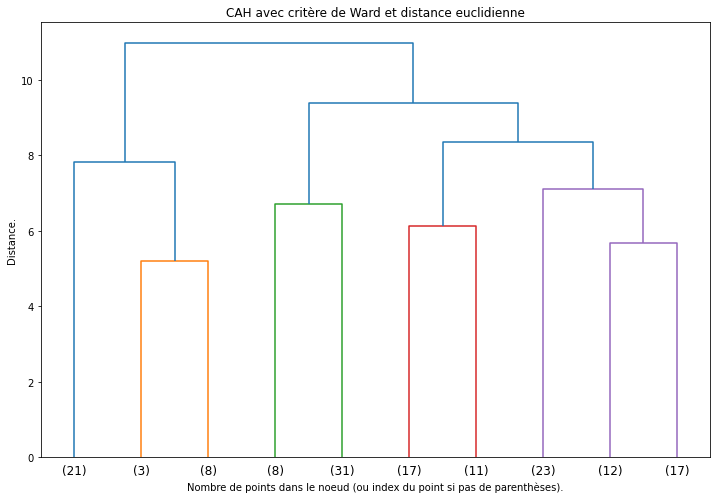
\includegraphics[width=\textwidth]{S4-Explicabilite_globale/figures/dendrogramme.png}
\caption{Dendrogramme de la Classification Ascendante Hiérarchique des 151 vecteurs supports protagonistes de la classe ``\textit{Discrimination : contrat étudiant}'', pour $10$ groupes au plus bas du dendrogramme. } \label{fig:dendrogramme}
\end{figure}

Sur les 151 points de données, la figure~\ref{fig:dendrogramme} montre que le regroupement en $10$ groupes donne des ensembles plutôt équilibrés, à l'exception d'un groupe de $3$ éléments et d'un groupe de $31$ éléments. En nous basant sur la figure~\ref{fig:dendrogramme}, nous considérons que le découpage en $5$ groupes est un niveau de zoom intéressant, avec des groupes à la fois équilibrés et un saut de taille correcte; notamment plus élevé que celui pour $4$ groupes.

% Résultat
En considérant $n=5$ groupes, et en appliquant le tri sur les paires via les vecteurs supports antagonistes, on obtient le tableau~\ref{tab:results_student_ant5}. Les 5 paires sont affichées, montrant des textes de taille variable. Les travaux du chapitre 3~\ref{C3} ont été employés pour mettre en avant les mots de fort poids d'attention, c'est à dire un poids supérieur à un seuil $t=0,15$. Les

\begin{longtable}{|p{0.06\textwidth}|p{0.1\textwidth}|p{0.8\textwidth}|}
    \caption{Exemples factuels pertinents pour la classe ``Discrimination : contrat étudiant'' et leurs exemples contrefactuels de la classe ``Légal'', tri effectué sur les vecteurs supports antagonistes. Les mots soulignés sont ceux remontés par les explications par attention.  } \label{tab:results_student_ant5} \\ \hline
    \textbf{Paire}       & \textbf{Type}     & \textbf{Texte}    \\ \hline
    \endfirsthead
    %
    \endhead
    %
    \multirow{2}{*}{1} & Exemple          & Votre profil :    Vous detenez des experiences verifiables avec les enfants, aupres de structures ou de particuliers   Votre mission, si vous l'acceptez :   Vous vous occupez des enfants au domicile des parents  Vous assurez le bien-etre des enfants jusqu'au retour des parents (maternage, change, soins, gouter, sortie d'\underline{ecole}/creche)  Vous organisez des activites d'eveil et jeux en fonction de l'age des enfants   Il vous faudra etre disponible :    Lundi Mardi Jeudi et Vendredi de 17h30 a  19h et le mercredi de 9h a  12h   Avantage :    Vous pouvez cumuler plusieurs missions  Un job proche de votre domicile  Des horaires compatibles avec votre emploi du temps vous permettant ainsi de cumuler deux emplois ou un job etudiant avec vos etudes.  \\ \cline{2-3}
                       & Contre - exemple & Votre mission, si vous l\&rsquo;acceptez : Vous vous occupez des enfants au domicile des parents  Vous assurez le bien-etre des enfants jusqu\&rsquo;au retour des parents (maternage, change, soins, gouter, sortie d\&rsquo;ecole/creche) Vous organisez des activites d\&rsquo;eveil et jeux en fonction de l\&rsquo;age des enfants  Il vous faudra etre disponible : En moyenne 2 fois par semaine de 6h15 a 13h30 ou de 16h a 20h30 (un planning mensuel vous sera fourni par la famille)  Plusieurs disponibles en complement, a proximite Agence: Metz Categorie: Garde d'enfants de moins de 3 ans Ville:Delme Type de poste:Temps partiel Periode:Annee scolaire 2019-2020Competences:Debutant(e) accepte(e)  \\ \hline
    \multirow{2}{*}{2} & Exemple          & Recherche baby-sitter à domicile à \underline{CHATOU} pour 7,8 heures de travail par semaine pour baby-sitter 1 enfant, 7 ans.\textgreater{}br\textgreater{}Tâches confiées : garde d'enfants/baby-sitting, goûter, aide à la toilette, suivi des devoirs, préparation et prise des repas, accompagnement dans les déplacements.\textgreater{}br\textgreater{}Rémunération : 10,50 € brut/heure.\textgreater{}br\textgreater{}Horaire du baby-sitting : Du 05/09/18 au 17/10/18 puis du 07/11/18 au 19/12/18 puis du 09/01/19 au 20/02/19 puis du 13/03/19 au 17/04/19 puis du 08/05/19 au 29/05/19 puis du 05/06/19 au 03/07/19: Le mercredi de 08h30 à 18h00.   \\ \cline{2-3}
                       & Contre - exemple & Recherche baby-sitter à domicile à MARSEILLE pour 0,9 heures de travail par semaine pour baby-sitter 2 enfants, 8 ans, 11 ans.\textgreater{}br\textgreater{}Tâches confiées : garde d'enfants/baby-sitting, sortie d'école.\textgreater{}br\textgreater{}Rémunération : 9,88 € brut/heure.\textgreater{}br\textgreater{}Horaire du baby-sitting : Du 04/09/18 au 04/10/18 puis du 27/11/18 au 29/11/18 puis du 22/01/19 au 24/01/19 puis du 19/03/19 au 21/03/19 puis du 14/05/19 au 13/06/19:\textgreater{}br\textgreater{}1 semaine sur 4 sera travaillée.    \\ \hline
    \multirow{2}{*}{3} & Exemple          & 35 H/Semaine \underline{Etudiants} acceptés.  \\ \cline{2-3}
                       & Contre - exemple & 35 H/Semaine minimum Etudiants acceptés. \\ \hline
    \multirow{2}{*}{4} & Exemple          & \underline{Etudiant}(e), à la retraite ou en activité à temps partiel, nous serons enchantés de vous compter parmi notre équipe, à bientôt Dans le cadre de cette mission, le véhicule est exigé pour le transport des enfants.  \\ \cline{2-3}
                       & Contre - exemple & Etudiant(e) de niveau Bac+4, vous préparez un diplôme en sécurité des systèmes informatiques / gestion de projet.  \\ \hline
    \multirow{2}{*}{5} & Exemple          & Lieu de travail : Montpellier et alentours (Castelnau, Jacou, Clapiers, Montferrier, Teyran, Saint Clément de Rivière, Saint Gély du Fesc, Le Crès.)Profil recherché :v  Débutant acceptév  Ponctualité, Sérieux et Esprit d'initiativev  Autonomie et Capacité d'adaptationv  Sens de la relation clientèle, Sociabilitév  Permis B indispensable Si vous êtes \underline{Etudiant}, merci de vous assurer de la régularité de vos disponibilités sur une période de longue durée (au moins 8 mois).    \\ \cline{2-3}
                       & Contre - exemple & TERRE \&amp; MER INTÉRIM recherche, pour un de ses clients, 8 OPÉRATEURS NETTOYAGE INDUSTRIEL (H/F) sur Port de commerce à BRESTVos missions : - Nettoyage / Dégazage de cuves de Bateaux- Manutention- Une réunion / formation sécurité sera assurée par le client Durée de la mission : 1 semaine   TERRE \&amp; MER INTÉRIM recrute le profil suivant :- Carte d'identité obligatoire- Débutant / Etudiant accepté,Autonome, motivé(e), organisé(e), courage  \\ \hline
\end{longtable}

Le tableau~\ref{tab:results_student_pro5} présente le même tri effectué sur les vecteurs supports protagonistes. une partie des paires ont déjà été remontées par le tableau~\ref{tab:results_student_ant5} à savoir les paires 1, 3 et 4 et ne sont donc pas réaffichées. Comme dans le tableau précédent, les mots de poids d'attention élevé sont mis en gras.

\begin{table}
    \caption{Exemples factuels pertinents pour la classe ``Discrimination : contrat étudiant'' et leurs exemples contrefactuels de la classe ``Légal'', tri effectué sur les vecteurs supports protagonistes. Les mots en gras sont les mots remontés par les explications par attention. Les paires 1, 3 et 4 tu tableau~\ref{tab:results_student_ant5} sont également remontées, et non affichées ici dans un souci de clarté.} \label{tab:results_student_pro5}

    \begin{tabular}{|p{0.1\textwidth}|p{0.1\textwidth}|p{0.8\textwidth}|}
        \hline
        \textbf{Paire}              & \textbf{Type}             & \textbf{Texte}                              \\ \hline
        \multirow{2}{*}{6} & Exemple          & Vous gererez en autonomie le trajet creche/domicile, realisez des \textbf{activites} diverses (activite manuelles, lectures \&hellip;), suivi de \textbf{devoirs} pour le plus grand, temps calme jusqu\&rsquo;au retour des parents   Experience exigee d\&rsquo;1 an minimum  en garde d\&rsquo;enfants chez des particuliers (sortie d\&rsquo;ecole, aides aux devoirs, babysitting) ou en structure collective (centre de loisirs, creche\&hellip;)   Formation appreciee  dans le secteur (CAP, BEP carrieres sanitaires et sociales, Bac Pro ASSP, BAFA\&hellip;)   Horaire d\&rsquo;intervention : Lundi/Mar/Jeu./Ven : 16h30 \&ndash; 18h30 et Mercredi 13h30-18h30 ou 11h30 \&ndash; 16h   Remuneration : 9,88 a 10,10 \&euro;/ H (variable selon experience et formation)   en CDI a pourvoir des la rentree 2018   Vous etes etudiant(e)s, s ou salarie(e)s a temps partiel ? Devenez Babychou-sitter(trice) en envoyant votre CV ! \\ \cline{2-3}
                           & Contre - exemple & Vous gererez en autonomie le trajet ecole/domicile, realisez des activites diverses (jeux de societe, lectures, sorties au parc\&hellip;), et parfois les repas et le bain   Experience exigee d\&rsquo;1 an minimum  en garde d\&rsquo;enfants chez des particuliers (sortie d\&rsquo;ecole, aides aux devoirs, babysitting) ou en structure collective (centre de loisirs, creche\&hellip;)   Formation obligatoire  dans le secteur (CAP, BEP carrieres sanitaires et sociales, Bac Pro ASSP, BAFA\&hellip;)   Horaire d\&rsquo;intervention : Semaine 1 Lundi/Mardi/Jeudi/vendredi 16h30-19h + Mercredi 9h -19h + Semaine 2 Jeudi/vendredi 16h30 \&ndash; 19h   Remuneration : de 10.10 a 10.88 \&euro;/ H (variable selon experience et formation)   en CDI a pourvoir des la rentree 2018   Vous etes etudiant(e)s, s ou salarie(e)s a temps partiel ? Devenez Babychou-sitter(trice) en envoyant votre CV !  \\ \hline
        \multirow{2}{*}{7} & Exemple          & Recherche: Opérateur de production - contrat \textbf{Etudiant} (H/F)PARTNAIRE recrute pour son client  MAITRE COQ qui est une filiale du groupe agroalimentaire LDC, groupe en pleine croissance, solide et pérenne, connu pour ses marques Loué, Le Gaulois, Maître Coq, Marie et Traditions d'Asie.   \\ \cline{2-3}
                           & Contre - exemple & \&lt;br\&gt;\&lt;br\&gt;\&lt;br\&gt;Dans le cadre de sa politique diversité, Manpower étudie, à compétences égales, toutes candidatures dont celles de personnes en situation de handicap Profil :Etudiant opérateur approvisionneur (H/F)Poste en INTERIMEntreprise :Activité du client : Agroalimentaire   \\ \hline
        \end{tabular}
\end{table}

Le premier exemple, soit la paire 1 dans le tableau~\ref{tab:results_student_ant5}, présente une offre longue, rejetée principalement par la présence du terme ``école''. Le contre-exemple présente une séquence de mots fortement similaire, mais avec un problème d'encodage du texte, présentant la séquence de texte \textit{``\&rsquo;''} juste avant le mot école.
Une analyse plus approfondie de cette paire permet de constater un fort poids d'attention pour le mot école dans l'exemple : $0,98$. Dans le contre-exemple, le mot école a un poids d'attention de $0,33$. Toutefois, en supprimant la séquence \textit{``\&rsquo;''}, le poids d'attention du mot école augmente fortement et passe à $0,98$. Cet exemple met en avant la problématique d'une captation de textes de qualité variable, avec la présence de séquence de caractères qui bruitent les phrases. Ici,  \textit{``\&rsquo;''} correspond à une apostrophe, en langage XML ou HTML.
% exemple : [(49, ('ecole', 0.9784968))]
% [(37, ('ecole', 0.33080584)), (60, ('disponible', 0.29758972))] avec risq
% [(36, ('ecole', 0.9801989))] sans risq

La seconde paire d'exemples du tableau~\ref{tab:results_student_ant5} montre un cas typique de faux positif, avec un mot peu connu : la ville de \textit{``Chatou''}. En contre-exemple, une offre similaire pour la ville de Marseille, plus grande donc à priori plus connue, ne pose pas de problème.

Les paires 3, 4, 5 et 7 montrent que le modèle déclenche un rejet autour du mot ``\textit{étudiant}'' au singulier et pluriel. Cependant, le contexte joue énormément. Les différences sont parfois minimes, comme pour la paire 3 du tableau~\ref{tab:results_student_ant5} où l'ajout du mot ``minimum'' rend la phrase acceptable.

La paire 6 du tableau~\ref{tab:results_student_pro5} montre deux offres d'un même recruteur. Elle met en avant les mots ``activités'' et ``devoirs'' de la phrase rejetée; non présents dans le contre-exemple associé. Une hypothèse, non vérifiée, est-ce que ces mots rapportent au champ de la garde d'enfant, a l'instar du mot école vu dans la paire 1. Hors, les offres de garde d'enfants comportent régulièrement des mentions de contrats étudiants, ce qui peut amener à un biais dans l'apprentissage de cette classe. Cet exemple a largement bénéficié de l'application des explications locales. En effet sans celles-ci, nous aurions cherché à analyser la partie du texte portant sur la mention ``étudiant'', alors qu'elle est identique pour l'exemple et le contre-exemple.

% Conclusion de cette analyse :
La caractérisation proposée a permis de mettre en avant la définition des frontières de la classe ``\textit{Discrimination : contrat étudiant}''.
Certains termes ont été mis en avant en tant que déclencheurs de rejet. Une analyse d'un expert du domaine est encore nécessaire pour définir les expressions acceptées ou non; notamment dans notre exemple avec le mot ``étudiant'' et ses variantes (``étudiants acceptés'', ``contrat étudiant'' etc.).
D'autres termes amènent à penser qu'il existe un fort biais menant au rejet d'offres comportant des mots associés à la garde d'enfants.
D'autres éléments ajoutent du bruit à la phrase analysée. Ce sont des noms propres peu connus, ou des problèmes de qualité des données. Ces éléments apportent des pistes d'amélioration du prétraitement des textes. Une piste consiste à remplacer tous les noms de localisations par un mot commun, tel que cela est fait en reconnaissance d'entités nommées. Les balises HTML et autres artefacts glissés dans le texte peuvent également être recherchés et supprimés via des expressions régulières.


\section{Conclusion}

Dans cette contribution, nous proposons un protocole de caractérisation par l'exemple de modèles complexes, de manière ad-hoc.  Avec ce protocole, nous souhaitons fournir aux utilisateurs des éléments concrets pour les aider à créer leurs propres modèles mentaux.

Ce protocole consiste à extraire des éléments clés des données d'apprentissage, et à les trier pour présenter un ensemble digeste d'éléments. Ces éléments permettent à l'utilisateur ou utilisatrice effectuant la caractérisation du modèle de mieux appréhender ses frontières de décision.

% Avantages
La méthode de caractérisation proposée ne requiert pas d'architecture spécifique (méthode ad-hoc).
La stratégie est modulaire, permettant ainsi de modifier son implémentation à divers niveaux, la rendant flexible et adaptable.
L'implémentation proposée s'appuie sur les données réelles extraites du jeu d'entraînement du modèle. Dans la mesure du possible, elle fait appel à des algorithmes de complexité limitée.

% limites
Toutefois, cette implémentation nécessite d'avoir accès aux données d'entraînement, ce qui n'est pas toujours possible.

L'application de ce protocole a également mis en évidence ses limites.
Ainsi, nous avons profité du travail sur un modèle transparent pour récupérer les mots déclencheurs de rejet de manière fine. Sans l'ajout d’explications locales, l'analyse n'aurait pas été aussi poussée.
L'analyse manque d'une analyse qualitative fine, réalisée avec des experts du domaine fonctionnel. Il aurait également été intéressant de pouvoir appliquer une correction du jeu d'entraînement, issu d'une telle analyse, et mesurer un éventuel gain (ou perte) de performance.
Enfin, l'analyse est effectuée classe par classe. Nous présentons ici l'application sur une seule classe, qui comporte déjà un nombre important d'éléments. Il serait intéressant de mener une étude sur la capacité de génération d'un modèle mental complet par des personnes utilisant cet outil.

% possibilités d'améliorations
Notons que ce chapitre présente une première application, qui n'a pas été comparée aux méthodes de la littérature. Mettre en place une comparaison robuste serait souhaitable avant de chercher à la peaufiner.
Par ailleurs, il faudrait comparer, entre les GAN et la méthode présentée, le temps de calcul pour obtenir des explications par le contre-exemple.

% ouverture
Les préoccupations de sobriété des algorithmes, communément rassemblées sous le nom de \textit{green it}, font partie intégrante d'une volonté de développer des algorithmes et outils plus vertueux. \`A ce titre, nous nous sommes efforcés de privilégier des pistes peu coûteuses mais suffisamment intéressantes.
XAI et éthique étant souvent liés, nous espérons que la sobriété énergétique sera un axe fort dans le développement de la communauté XAI.

\boitemagique{Résumé}{
\begin{itemize}
    \item[\checkmark] Une stratégie de caractérisation d'un modèle a été présentée
    \item[\checkmark] Nous présentons une preuve de valeur d'une application de cette méthode à un cas d'usage
    \item[\checkmark] L'application met en avant des éléments de compréhension du comportement du modèle
    \item[\checkmark] L'application met en avant des limites de la méthode, qui perd en intérêt sans explications locales
    \item[\checkmark] Un comparatif qualitatif robuste avec d'autres méthodes de la littérature est nécessaire
\end{itemize}
}


\clearemptydoublepage

\chapter[Intégration à l'environnement industriel]{Intégration à l'environnement industriel}

\boitemagique{Dans ce chapitre}{
Ce chapitre présente les liens entre explicabilité et problématiques de Pôle emploi. Nous décrivons le cadre logiciel \textit{Gabarit} et les développements de la thèse réalisés dans ce dernier. Les apports de la démarche d'explicabilité aux  engagements éthiques sont présentés. Enfin, nous proposons un guide des méthodes d'explicabilité dédiées à l'industrie.
}

% intro
Ce chapitre présente l'intégration des travaux de cette thèse dans l'environnement industriel de Pôle emploi.
% Quoi
Les liens entre ces travaux et l'entreprise sont multiples. D’un point de vue technique les contributions d’explicabilité présentées sont implémentées dans l'infrastructure de développement de Pôle emploi : \textit{Gabarit}. %outil open source destiné à la mise en production de modèles d'apprentissage automatique.
D’un point de vue des enjeux éthiques autour de l'IA chez Pôle emploi, ce chapitre participe à la mise en place et à la réponse aux exigences de la charte éthique IA.

% Objectif du chapitre
Nous présentons l'apport cette thèse à l'outil, en section~\ref{C6:gabarit}. La section~\ref{C6:ethique}, montre la contribution de la thèse pour la mise en œuvre de la charte éthique Pôle emploi. Enfin, un guide est proposé en section~\ref{C6:guide} afin de choisir d'une méthode d'explicabilité dans un contexte industriel.

\section{Gabarit} \label{C6:gabarit}

% intro
Dans cette section, nous présentons \textit{Gabarit}\footnote{\url{https://github.com/OSS-Pole-Emploi/gabarit}}, un outil open source créé par Pôle Emploi. Sous la forme de module python, il permet de générer des projets d'apprentissage automatique prêts à l'emploi.
% Pourquoi
Il permet ainsi d'uniformiser les pratiques, favoriser le partage, accélérer la mise en production des modèles d'IA.
% Objectif du chapitre
Dans ce chapitre, nous présentons l'historique de l'outil, sa philosophie, et comment s'y intègrent mes travaux de thèse.

\subsection{Historique} \label{C6:historique}

% participation active mais avant la thèse
Les premiers travaux de création d'outillage communs autour de la donnée démarrent en 2018. Ils sont liés au besoin du département \textit{Agence Data Services} d'unifier les processus spécifiques de nettoyage de données textuelles. Cet outil, nommé \textit{Words'n'fun}, présente un ensemble de fonctions python pour le prétraitement de textes\footnote{\url{https://github.com/OSS-Pole-Emploi/words_n_fun}}.
% participation active mais avant la thèse
Ce besoin d'uniformisation des bonnes pratiques s'étend au développement de modèles d'IA en NLP. La volonté est de faciliter leur mise en production et le transfert du projet d'une personne à l'autre. Le \textit{Template NLP} est créé en 2019, en tant que projet git à télécharger. Il est axé sur l'entraînement, la sérialisation et la mise à disposition de modèles d'IA. L'outil est un générateur de projets, il embarque et intègre divers outils open source pour
historiser les données avec \textit{Data Version Control} (DVC)\footnote{\url{https://dvc.org/}} et les prétraiter avec \textit{Words'n'fun}),
effectuer l'apprentissage automatique (\textit{Scikit-Learn}\footnote{\url{https://scikit-learn.org/}}, \textit{Tensorflow}\footnote{\url{https://www.tensorflow.org/}}  et \textit{Torch}\footnote{\url{https://pytorch.org/}}),
aider au suivi des modèles (\textit{MLflow}\footnote{\url{https://mlflow.org/}}, \textit{Artifactory}\footnote{\url{https://jfrog.com/fr/artifactory/}})
ainsi qu'un démonstrateur \textit{Streamlit}\footnote{\url{https://streamlit.io/}}.

Pour faciliter sa prise en main par les scientifiques des données de l'entreprise, une formation au travers de tutoriels interactifs est mise en place. Les travaux de cette thèse sont réalisés en utilisant cet outil, contribuant ainsi directement à l'ajout de fonctionnalités d'explicabilité.

En 2020 et 2021 sont intégrés au \textit{Template NLP} les \textit{Template vision} et \textit{Template numérique}, gérant respectivement les données tabulaires et les images. L'outil évolue selon les besoins et les contraintes de mise en production.
Dès le démarrage du projet, son ouverture à la communauté open source est considérée. En 2022, le service juridique donne son aval pour que le code soit rendu disponible sous licence copyleft; ce qui donne lieu à des travaux de refonte. Un des points principaux est la traduction en anglais, car le code interne Pôle emploi est historiquement écrit en anglais avec des commentaires français, ce qui limite le partage à la communauté. Les tests sont améliorés pour consolider le projet, et l'installation est facilitée en partageant le projet sous forme de module python. Le tout est rendu public en 2022 sous le nom \textit{Gabarit}.

% D'abord le template NLP avec la gestion sklearn/tensorflow (torch par la suite) et intégration dvc/mlflow/words\_n\_fun; gestion des embeddings, des différents datasets etc...
% Ensuite on a rajouté le template vision (en avance de phase) pour tout ce qui est CV, puis le template numerique pour les données tabulaires plus classiques

L'outil \textit{Gabarit} est composé de 2 éléments : le générateur de projets et le projet généré à utiliser. Le générateur est présenté dans la section suivante, et le projet généré est présenté à la suite.

\subsection{Le générateur de projets}

Le générateur de projets permet de créer un projet d'IA en une ligne de commandes. Il gère notamment les formats de données lus et sérialisés (encodage, séparateur de colonne des fichiers csv...), et les éventuels outils à configurer tel que DVC.

Une fois le module installé (ou mis à jour), il est directement possible de créer un nouveau projet. La ligne de commande permet de générer un projet d'analyse de textes (\textit{generate\_nlp\_project}), d'images (\textit{generate\_vision\_project}) ou de données tabulaires (\textit{generate\_num\_project}).
D'autres précisions optionnelles sont disponibles pour la gestion du projet : intégration de DVC, configuration spécifique (encodage...), etc. Plus de détails sont donnés dans la documentation du projet.

Le générateur repose sur une arborescence de fichiers ``templates'' correspondant chacun à une typologie de données (texte, image et tabulaire). Chaque \textit{template} contient le code source presque prêt à l'emploi : il ne reste qu'à remplacer le nom du projet, à la manière d'un texte à compléter, ce qui est effectué automatiquement lors de la génération du projet.
% En complément, de l'arborescence de fichiers ainsi complétée qui va constituer le cœur du projet IA, celui-ci va également comporter de nombreuses suites de tests permettant de valider le bon fonctionnement des fonctionnalités proposées ainsi que des jeux de données jouets permettant de faciliter la prise en main du code généré au travers d'un tutoriel.
Le générateur peut ainsi créer le projet souhaité avec le nom et l'emplacement donnés, ainsi que les spécifications optionnelles. Tous les fichiers sont générés pour être prêts à l'emploi.

\subsection{Architecture du projet généré}

Une fois le projet généré et installé, tout le code du projet peut être modifié par le scientifique des données qui y a un accès direct, à la différence d'outils plus graphiques tels que Dataiku. Il reste possible d'intégrer par la suite tout module python souhaité. C'est également le moment idéal pour démarrer l'historisation sur \textit{git}, si cela n'a pas déjà été mis en place.

Une fois le projet installé, il ne reste plus qu'à intégrer les données souhaitées. Des fonctions sont à disposition pour prétraiter les données. Des architectures de modèles d'apprentissage automatique sont à disposition des utilisateurs,  basées sur le trio \textit{Scikit-learn}, \textit{Tensorflow}, \textit{Pytorch}.
Il est possible d'entraîner directement un de ces modèles, d'ajuster leur architecture, ou encore d'en créer un nouveau, le tout avec très peu de modifications de code à effectuer. Les architectures de modèle couvrent à la fois l'apprentissage automatique et profond.

La figure~\ref{fig:api_gabarit} illustre les six fonctionnalités liées directement au modèle et à son cycle de vie, à savoir : le définir, l'entraîner (méthode \textit{fit}), l'enregistrer et recharger (\textit{save} et \textit{load\_model}), l'utiliser pour prédire un résultat (\textit{predict}) et expliquer celui-ci (\textit{explain}).
\begin{figure}[htpb!]
\centering
\includegraphics[width=\textwidth]{S5-Presentation_du_template_nlp/figures/usage_gabarit.png}
\caption{Illustration des fonctionnalités de \textit{Gabarit} pour un modèle : définition, entraînement, sérialisation, chargement, inférence et explication.}
\label{fig:api_gabarit}
\end{figure}

L'architecture de chaque modèle est disponible dans un script associé, ce qui permet notamment d'ajouter, supprimer, modifier des couches de réseaux.

Le projet intègre également des interfaces avec divers outils, notamment un démonstrateur via une page web, et la mise à disposition du modèle via \textit{artifactory} afin d'être utilisé dans différents services et outils.

Cet environnement a servi de base pour les développements des travaux présentés ici. De même, les travaux ont nourri l'outil \textit{Gabarit}. Nous présentons cet échange dans la section suivante.

\subsection{Intégration des travaux d'explicabilité}

Les travaux présentés ici sur l'explicabilité des algorithmes ont été développés dans \textit{Gabarit}. Le modèle à attention présenté en chapitre 4 a été conçu au sein de l'outil, ainsi que les développements liés aux explications globales. De même, le démonstrateur fourni a servi de base aux illustrations des différentes méthodes d'explications.

Réciproquement, une partie des avancées de cette thèse ont servi à enrichir l'outil. Le principal avantage est l'intégration directe d'une méthode d'explicabilité pour tout modèle, via la méthode \textit{model.explain}. L'explication est par défaut apportée par Lime~\cite{Ribeiro2016}, une méthode agnostique au modèle parmi les plus légères, et en moyenne plus rapide que les ancres utilisées dans les chapitres 3 et 4. Lime sert de premier point de référence pour les scientifiques des données. Notre état de l'art montre qu'il existe toutefois d'autres méthodes intéressantes.

L'architecture du modèle à attention utilisé y est mise à disposition en générant un projet d'analyse de textes, via la classe \textit{ModelEmbeddingLstmStructuredAttention}. Les explications par attention sont récupérables, à titre expérimental et pour cette classe uniquement, via la méthode \textit{model.explain\_indexes}. %À noter que cette partie de l'outil n'est pas passée par les mêmes tests rigoureux d'industrialisation que les autres modèles et méthodes.
L'intégration au fil de l'eau des contributions au cadre logiciel permet aux équipes de Pôle emploi ou autres utilisateurs de l'outil d'intégrer la notion d'explicabilité à tous les modèles d'IA.

Pour conclure brièvement sur cette section, \textit{Gabarit}, a accéléré la mise à disposition des développements effectués dans le cadre de cette thèse. En l'employant, nous avons facilité l'accès aux travaux d'explicabilité, pour les équipes de Pôle emploi, mais également à toute personne intéressée.

L'outil étant conçu pour faciliter la mise en production d'outils d'IA, il possède toutefois des contraintes non adaptées à un environnement de recherche pure. C'est un outil lourd, faisant appel à de nombreuses dépendances. Celles-ci sont ajustables grâce à la modification directe du code python, mais il est contre-productif de s'écarter totalement du cadre prévu. Ainsi, les premiers développements de cette thèse se sont faits avant l'intégration de Pytorch, ce qui a contraint à réaliser les développements sur tensorflow.

Les travaux mentionnés dans cette section ont été techniques, mais ce n'est pas le seul apport pour l'entreprise. La section suivante montre leur intérêt dans la réflexion éthique réalisée à Pôle emploi.

\section{\'Ethique} \label{C6:ethique}

L'éthique de l'IA est un enjeu présent à Pole emploi depuis 2018. La figure~\ref{fig:chronologie_ethique}  montre la chronologie et les grands points d'étape de la réflexion autour de ces enjeux. Les étapes auxquelles j'ai activement contribué, notamment en participant aux réunions d'avancement, sont encadrées en noir. L'éthique est d'abord abordée par le prisme de la maitrise des risques. Les premiers travaux mènent à la construction de la \textit{charte pour une IA éthique}~\cite{Pole2022}. C'est en parallèle et dans le même contexte que les travaux de la présente thèse sur l'explicabilité des algorithmes d'IA sont proposés, le sujet étant affiné au long de l'année 2019.
% 17% de la population de 15+ ans en situation d'illectronisme, enquête menée dans les Hauts de France en 2019, Insee, enquête TIC ménages 2019, RP 2016.

\begin{figure}[htpb!] % TODO trait + gros
\centering
\includegraphics[width=\textwidth]{S5-Presentation_du_template_nlp/figures/ethique_chrono.png}
\caption{ Chrolonogie des projets et évènements liés à l'éthique à Pôle Emploi depuis 2018. Les projets encadrés en noir sont ceux auxquels j'ai activement participé.}
\label{fig:chronologie_ethique}
\end{figure}

Ainsi, avec les réflexions entamées en 2018, la \textit{charte pour une IA éthique} fait son apparition dès 2020. Un premier point d'évaluation de l'existant est alors effectué dans la foulée.
La figure~\ref{fig:chronologie_ethique} montre l'accélération des travaux en 2021.
Un projet pilote met en place une première salve d'ateliers d'\textit{opérationnalisation} de la charte.

En début d'année, la création du \textit{Comité Consultatif \'Ethique de Pôle Emploi} (CCEPE) est actée. Ce comité externe est composé de dix experts d'horizons complémentaires : universitaires, représentants de syndicats et des usagers. Ce CCEPE a pour vocation d'accompagner et porter un regard externe critique sur les engagements et actions de l'établissement. Dans ce cadre, le CCEPE a dialogué activement avec les acteurs de Pôle emploi, me permettant de présenter l'avancée des travaux sur explicabilité.

Par la suite, les travaux de thèse d'Angela Ciocan sur la mesure de l'impact environnemental de l'IA démarrent.
Les risques éthiques liés à l'IA sont évalués de façon plus globale pour tous les sujets existants et à venir. Les ateliers de cotation de ces risques mêlent des profils techniques et managériaux. Ces cotations sont une première étape permettant l'opérationnalisation de la charte.

Par la suite, nous présenterons la charte et ses grands principes en section~\ref{C6:charte}. Sa mise en œuvre est traitée, de la cotation des risques à la l'établissement d'outils pour les acteurs des projets IA, en section~\ref{C6:ope_charte}.

\subsection{La charte éthique} \label{C6:charte}

La charte est publiée en interne dans un premier temps, puis publiquement en Novembre 2021. Elle est donc disponible sur le site de communication officiel de Pôle emploi\footnote{\url{https://tinyurl.com/charteIA}}. Elle est également en annexe en section~\ref{A:charte_pe}.
Cette charte répond au besoin de suivi interne, mais également à la volonté d'être auditables.

Les 7 axes de la charte :
\begin{enumerate}
    \item Finalité et légitimité des algorithmes,
    % Inadéquation entre les finalités des algorithmes et solutions d'IA, et les missions de PE telles que décrites dans l’article L5312 du code du travail
    \item L’humain au centre ; l’intelligence artificielle au service de l’humain,
    % Absence de compréhension du sens et des enjeux du recours à l'IA dans les solutions : méfiance, non-utilisation des solutions, etc. (culture change)
    \item Equité et non-discrimination,
    % Défaillance ou absence de mesures permettant de garantir l’équité de traitement entre les utilisateurs
    \item Liberté de choix,
    % Absence de temps laissé aux agents et aux usagers pour la prise de décision
    \item Transparence,
    % Défaillance ou absence dans la capacité à expliquer le fonctionnement d'un algorithme et ses résultats (règles que se donne l'algorithme)
    % Défaillance ou absence d'explication détaillée et sous forme intelligible du résultat algorithmique par le responsable de traitement
    \item Sécurité,
    % Défaillance ou absence de la qualité de la collecte et du traitement des données
    \item Impact environnemental.
    %Absence de mise en place d'un indicateur multicritère d’impact en collaboration avec l’INR
\end{enumerate}
% + risques associés ajoutés

% Plus éloigné ; en parler un peu
\paragraph{Finalité et légitimité des algorithmes}
Cet axe implique d'utiliser les outils d'IA à bon escient, dans le but de fournir un service bénéfique ou de lutter contre les actes de malveillance.

\paragraph{L’humain au centre ; l’intelligence artificielle au service de l’humain}
Les outils sont créés pour accompagner l'humain dans ses tâches habituelles. Pôle emploi indique dans sa charte s'engager à fournir ``une explication sur le fonctionnement d'un service ou une aide à la décision'' ainsi que ``des actions d'accompagnement et de sensibilisation [...] à l'intelligence artificielle'' aux utilisateurs internes (\textit{agents}) et externes (\textit{usagers})~\cite{Pole2022}.

\paragraph{Equité et non-discrimination}
Il s'agit ici à la fois de reconnaitre que l'IA peut ``reproduire, renforcer ou générer des biais discriminatoires'', et veiller à limiter l'impact de ceux-ci~\cite{Pole2022}. Le contexte applicatif de l'établissement est à risque du fait de biais humains présents dans le monde du travail. Les discriminations à l'embauche ou les métiers dits ``genrés'' en sont des exemples.

\paragraph{Liberté de choix}
Les décisions prises par un algorithme peuvent toujours être modifiées par un humain, et les utilisateurs ont accès à un interlocuteur pour demander un tel recours. Il est toujours possible d'ignorer les recommandations des algorithmes d'aide à la décision. En d'autres termes, l'humain a le dernier mot.

\paragraph{Transparence}
Cet axe répond aux exigences du RGPD et de la loi pour une république numérique~\cite{Legifrance2016}.
Il comprend le recueil du consentement éclairé des utilisateurs pour collecter et traiter leurs données.
La transparence concerne ici l'information aux utilisateurs lorsqu'iels ont à faire à un outil automatique, potentiellement basé sur l'IA. Cette exigence couvre notamment les agents conversationnels (ou ``chatbots'').
La charte indique très clairement que l'indication de l'utilisation d'un service d'IA s'accompagne de la ``capacité d'expliquer de la façon la plus compréhensible possible son fonctionnement et ses résultats''~\cite{Pole2022}.
% https://www.legifrance.gouv.fr/codes/article_lc/LEGIARTI000034195881 article R. 311-3-1-2 du Code des relations entre le public et l'administration
% https://www.legifrance.gouv.fr/codes/article_lc/LEGIARTI000033205535/  l'article L. 311-3 du Code des relations entre le public et l'administration

\paragraph{Sécurité}
La sécurisation concerne le traitement de données personnelles et sensibles, les paiements et la lutte contre les attaques (fraudes, arnaques, vol de données). Dans le cadre de l'IA, il s'agit notamment de valider l'usage de données personnelles et sensibles, si nécessaire les anonymiser. La sécurisation des services passe également par la vérification de leur résistance aux attaques adversaires. % TODO verif que attaques adversariales décrites avant, si oui crossref

\paragraph{Impact environnemental}
Dans une démarche d'usage responsable des outils à disposition, Pôle emploi reste attentif à l'impact et au coût environnemental des solutions développées. La démarche étant déjà entamée pour des développements hors IA, il s'agit ici d'une adaptation des bonnes pratiques existantes au développement, spécifique, des modèles d'apprentissage automatiques et profonds.

% Ici faire référence aux chapitres y afférent
Les travaux présentés dans ce manuscrit s'inscrivent directement dans deux des axes de la charte. Pour respecter les engagements des axes de \textit{l'humain au centre}, et de la \textit{Transparence}, il faut être en mesure d'expliquer le fonctionnement des algorithmes d'IA utilisés, dans leur fonctionnement global mais également lors de recours pour un résultat spécifique.


\subsection{Mise en œuvre de la charte} \label{C6:ope_charte}

La création de la charte est une première étape, mais son existence ne suffit pas à rendre les travaux entamés et révolus plus éthiques. Après une première étude sur un projet pilote, la mise en œuvre globale de la charte s'est faite en deux temps.

%  C:\Documents\Expertise XAI, Ethique\20201027_IE_Evaluation éthique_Mails_V1.6
Le projet pilote étudié porte sur l'analyse de mails afin d'assister les agents Pôle emploi. L'objectif est d'apposer une étiquette à chaque mail reçu par un conseiller : s'agit-t-il d'une demande de rendez-vous ? D'une réclamation ? Ces étiquettes permettent aux agents de s'organiser et construire leur planning plus facilement, en traitant ensemble toutes leurs demandes de rendez-vous, par exemple.  Ce projet pilote à l'avantage de faire appel à de nombreuses notions d'éthique (sécurité des données, non-discrimination, assistance et non remplacement du travail des conseillers...).
L'étude met en avant les caractéristiques spécifiques de ce projet avec ses acteurs, les données traitées etc. Les sept axes de la charte sont abordés un à un, et les points d'attention sont abordés avec les risques associés, les mesures déjà mises en place et les améliorations envisageables.

% 4. a) Ethique > 3 > carto
Les travaux de mise en œuvre de la Charte se sont par la suite généralisés à tous les cas d’usage IA de Pôle emploi.
La première étape a été la cotation des risques associés à chaque axe de la charte, selon leur probabilité et leur impact. Un risque est, par exemple une \textit{défaillance ou absence dans la capacité à expliquer le fonctionnement d'un algorithme et ses résultats (règles que se donne l'algorithme)}.
La probabilité d'occurrence $P$ de ce risque est quantifiée entre $1$, très peu probable, et $4$, fréquent. Les impacts sont également notés entre $1$ pour un impact faible, et $4$ pour un impact capital. Ces impacts sont évalués au travers de $6$ catégories:
\begin{enumerate}
    \item l' \textbf{image}, interne et médiatique, de l'établissement,
    \item les \textbf{finances} englobant les risques de pertes financières ou dépenses imprévues,
    \item \textbf{réglementaire}, allant du non-respect de la charte jusqu'au risque pénal,
    \item la réalisation des \textbf{missions}, comprenant les retards, la non réalisation des missions confiées,
    \item le \textbf{climat social} interne, comprenant les tensions pour les agents, allant jusqu'au risque de grève,
    \item l'\textbf{humain}, prenant en compte les agents et les usagers (demandeurs d'emploi et recruteurs).
\end{enumerate}
Ces impacts sont cotés collégialement grâce à un panel d'agents référents techniques, métiers, décisionnaires. La gravité $G$ du risque est calculée en fonction des cotations selon l'équation :
\begin{equation}
    G = P * \frac{I_{Image} + I_{Finance} + I_{Reglementaire} + I_{Mission} + I_{Social} + I_{Humain}}{6}
\end{equation}
Le risque est considéré peu grave lorsque $G \in [1, 4[$, et préoccupant lorsque $G \in [12,16]$.


À titre d'illustration, sans les travaux de cette thèse, la gravité de ce risque est de $4* (3+1+4+3+3+4)/6 = 12 $.
Avec la prise en compte de ces travaux, la gravité devient $ 1* (3+1+4+3+3+4)/6 = 3 $. Le risque, auparavant préoccupant, est alors peu grave. Cette illustration est tirée de la documentation interne de Pôle emploi, les chiffres sont à titre d'illustration seulement~\cite{Pole2021}.

La seconde étape de cotation consiste à déterminer les actions associées aux risques détectés, afin de diminuer l'impact de ceux-ci. Les actions peuvent diminuer les impacts ou la probabilité d'occurrence des risques. Ces actions sont globales, générales afin de s'adapter à tout projet. Reprenons le risque d'incapacité à expliquer un algorithme. Une action liée peut être \textit{Utiliser lorsque c'est possible des algorithmes et des solutions d'explicabilité afin d'être transparent sur les décisions prises}. Ces actions globales sont complétées par des précisions opérationnelles : tâches à mener, acteurs impliqués, moyens nécessaires et moment privilégié pour réaliser l'action. Dans l'exemple mentionné portant sur l'explicabilité, les travaux présentés dans ce manuscrit ont servi de base aux réflexions, apportant une vision des solutions existantes, et une preuve de première application.

%  s'établit en quatre phases synchronisées avec la vie du projet, comme le montre la figure
% \begin{figure}[htpb!]
% \centering
% \includegraphics[width=\textwidth]{S5-Presentation_du_template_nlp/figures/phases_etude_ethique.png}
% \caption{Les quatre phases d’études}
% \label{fig:chronologie_ethique}
% \end{figure}

% Conclusion : avancées, limites
Les travaux sur l'éthique ainsi que la cartographie des risques présents ont bénéficié, pour deux des sept axes de la charte, des réflexions engagées ici. Nous avons montré que nous pouvons réduire les risques rencontrés, en passant d'une volonté d'explicabilité à une application concrète de méthodes d'explications sur nos données, présentés en chapitres 2 et 4. Ces avancées nécessitent toutefois une priorisation et un suivi adéquats par les personnes en charge des différents projets. Nous conclurons cette section en soulevant le questionnement suivant : le devoir d'expliquer un résultat ou le fonctionnement d'un service doit-il être exigé uniquement lorsque ce dernier est basé sur des algorithmes d'intelligence artificielle ?

De manière concrète, et issue des savoirs engrangés dans cette aventure de trois ans, nous proposons à cet effet un guide permettant de faire le tri parmi les nombreuses méthodes d'explicabilité, en fonction des objectifs à atteindre.

\section{Comment choisir une méthode d'explicabilité ?} \label{C6:guide}

Cette section présente un guide permettant de déterminer les caractéristiques souhaitées pour une méthode d'explication. Les éléments de la section~\ref{C1:typologie} sont repris et organisés afin d'aider à la détermination de caractéristiques idéales pour un projet donné, en fonction de ses contraintes. Ce guide est inspiré de travaux existants~\cite{Vermeire2021}, simplifié et adapté au contexte industriel.

% objectif
Cette section fournit ainsi des outils qui aideront le lecteur ou la lectrice à déterminer ses besoins, et \textit{in fine} à sélectionner un panel restreint de méthodes de la littérature qui conviendront le mieux à ces besoins.
% plan


\paragraph{Guide des caractéristiques recherchées}
% quoi
Pour déterminer les systèmes d'explication préférables dans un projet, il faut au préalable déterminer les caractéristiques recherchées.
% comment
Pour déterminer ces caractéristiques, il faut avoir en tête l'objectif, le public, et le contexte de réception des explications. Il est possible que pour un même modèle d'IA, plusieurs besoins d'explicabilité soient détectés, à des moments de vie différents.
Dans ce cas, l'exercice proposé dans cette section est à réaliser pour chaque besoin.

% objectifs
Cette section propose un guide, permettant de définir les caractéristiques souhaitées pour un système d'explication.
% plan
Chaque caractéristique vue en introduction est passée en revue, à savoir la portée, la stratégie, et le format d'explication.

\paragraph{Choix de la portée}
%facteurs dominants
Les données principales permettant de choisir la portée de l'explication sont les utilisateurs et leurs objectifs.
%rappel options
Tel que vu en introduction, une explication de portée globale permet de construire la confiance dans le modèle sur son comportement général. Elle est pertinente pour les phases de validation et d'appropriation du modèle.
Une explication locale permet de se concentrer sur un résultat, et est plus proche des conditions réelles de l'utilisation du modèle.

\begin{figure}[htpb!]
    \centering
    \includegraphics[scale=0.22]{S5-Presentation_du_template_nlp/figures/guide_portee.png}
    \caption{Illustration du choix de la portée selon l'utilisateur et l'objectif de ce dernier}% TODO  traduction
    \label{fig:guide_portee}
\end{figure}

% analyse guide
La figure~\ref{fig:guide_portee} montre les publics concernés, à savoir :
\begin{itemize}
    \item les régulateurs, qui s'assurent de la conformité des outils au regard de la loi,
    \item les gestionnaires du projet, qui s'assurent de l'efficacité du service rendu,
    \item les scientifiques des données, qui produisent les modèles,
    \item les experts du domaine, qui utilisent les outils ou assistent les personnes concernées,
    \item les personnes concernées par l'usage de l'outil, si celui-ci impacte leur vie.
\end{itemize}
Ces publics sont rattachés à leurs objectifs dans le cycle de vie d'un projet. Selon les organisations, les publics et objectifs peuvent varier, la figure~\ref{fig:guide_portee} sert de modélisation globale et doit être adaptée.

%exemple - détails - adaptation
Ainsi, dans la figure~\ref{fig:guide_portee}, un expert du domaine avec pour objectif de créer de la confiance dans un outil d'IA peut recevoir des explications globales ou locales. Les explications globales seront plutôt adaptées en phase de test et appropriation de l'outil, en amont de la mise en production. Les explications locales seront plus adaptées lors d'une utilisation en conditions réelles d'utilisation.

\paragraph{Choix de la stratégie}
% TODO Harold Peut-être citer un ou deux exemples de chaque type pour mieux comprendre les différentes familles ?
%facteurs dominants
La stratégie à adopter est déterminée par plusieurs facteurs tels que l'accès au système d'intelligence artificielle, sa phase de conception, et son architecture si elle est déjà choisie.
% rappel options
Les approches boites transparentes sont les plus contraignantes et les plus coûteuses à la conception, mais peuvent limiter les calculs de génération des explications à posteriori, et sont par nature fidèles au fonctionnement interne du modèle à expliquer.
Les approches boites grises sont également basées sur le fonctionnement du modèle, mais nécessitent des calculs à postériori et sont basées sur les architectures des modèles à expliquer. Elles nécessitent d'y avoir accès afin de générer l'explication.
Les approches boites noires sont les moins contraignantes, mais peuvent s'avérer coûteuses en calcul pour générer l'explication. Puisqu'il n'y a pas besoin d'avoir accès au modèle, elles sont également moins fidèles au fonctionnement interne du modèle que les autres stratégies.

% TODO Harold : figure utile ?
\begin{figure}[htpb!]
    \centering
    \includegraphics[scale=0.22]{S5-Presentation_du_template_nlp/figures/guide_strat2.png}
    \caption{Cercle des possibles des stratégies de la moins contraignante à la plus contraignante, du centre vers l'extérieur.}
    \label{fig:guide_strat2}
\end{figure}

La figure~\ref{fig:guide_strat2} illustre les stratégies à disposition. Au centre du cercle les stratégies boites noires (BN), sont applicables en toutes circonstances.
Lorsque les conditions sont réunies, les stratégies boites grises (BG) s'ajoutent au panel des méthodes applicables, l'étendue des méthodes à disposition est alors élargie.
Sur le même principe, les stratégies boites transparentes (BT) sont applicables sous certaines contraintes. Elles s'ajoutent alors aux autres méthodes, élargissant encore le cercle des possibles, comme l'illustre la figure\ref{fig:guide_strat2}.

\begin{figure}[htpb!]
    \centering
    \includegraphics[scale=0.22]{S5-Presentation_du_template_nlp/figures/guide_strat.png}
    \caption{Illustration du choix de la stratégie la plus transparente applicable selon les contraintes du projet.}
    \label{fig:guide_strat}
\end{figure}

% analyse guide
La figure~\ref{fig:guide_strat} présente les choix de stratégies possibles selon les contraintes du modèle.
Le choix le moins restrictif est celui de la boite noire, applicable dans tous les cas, car il se base sur les entrées et sorties du modèle. Il est notamment adapté si le modèle est développé en externe ou si son fonctionnement interne est inaccessible pour une raison ou une autre.
Si le modèle est accessible et déjà conçu ou si son architecture est déjà choisie, alors, en fonction de cette dernière, certaines méthodes en stratégie boite grise sont applicables. Sinon, il faut se reporter sur les méthodes boites noires.
Si le modèle reste à concevoir, il est possible de concevoir son architecture avec une approche boite transparente. Les approches boite grise et boite noire restent également une option.


\paragraph{Choix du format}

Afin de choisir un type de format où un autre, il faut étudier les données à disposition et cibler les besoins des utilisateurs. La figure~\ref{fig:guide_format} schématise le choix d'un format par rapport à un autre. Si le schéma permet de privilégier une solution ou une autre, le format des explications doit s'intégrer à l'interface de l'outil où elles apparaissent. La mise en avant de variables ou d'exemples s'appuie sur des éléments concrets. Ces méthodes conviennent à une utilisation en condition réelle.
Mettre en avant une partie du contenu particulièrement utile lorsque l'exemple entier est trop long à analyser (image, texte composé de plusieurs phrases).
Les règles sont plus facilement généralisables, et sont ainsi adaptées aux audits. Les explications générées contiennent des formats plus variés, et sont à envisager lorsque les informations souhaitées ne sont pas lisibles dans les données directement : génération d'une phrase d'explications, instances menant en erreur, extraction de motifs représentatifs etc.
Si le schéma permet de privilégier une solution ou une autre, le format des explications doit s'intégrer à l'interface de l'outil où elles apparaissent.
Le test d'utilisabilité tel que présenté en section~\ref{C3:test_u} est idéalement à réaliser en complément.

\begin{figure}[htpb!]
    \centering
    \includegraphics[scale=0.22]{S5-Presentation_du_template_nlp/figures/guide_format.png}
    \caption{Illustration du choix de format des explications selon les contraintes du projet.}
    \label{fig:guide_format}
\end{figure}

Une fois un ensemble de caractéristiques choisi, il est possible de se référer aux nombreuses méthodes de la littérature pour trouver un ensemble de méthodes d'explication candidates à  essayer.


% \subsection{Guide des méthodes de la littérature}
%
% La littérature est fournie. Le tableau~\ref{tab:eda_caracteristiques} reprend les éléments mentionnés ci-avant, en y associant les caractéristiques vues en section~\ref{C1:typologie}.
%
% \begin{table}[htpb!]
%     \caption{TODO - \textit{Format à valider} - Récapitulatif des méthodes de l'état de l'art et leurs caractéristiques associées.} \label{tab:eda_caracteristiques}
%     \begin{tabular}{|l|l|l|l|l|l|}
%         \hline
%         \textbf{Méthode}  & \textbf{Référence} & \textbf{Portée}& \textbf{Format} & \textbf{Stratégie}   & \textbf{Données} \\ \hline
%         Cartes de modèles &~\cite{Mitchell2019} & Globale & Générée & Boite grise & Toutes  \\ \hline
%         Ancres          &~\cite{Ribeiro2018}    & Locale  &  Règle  & Boite noire &  Toutes \\ \hline
%                           % &              &         &         &             &         \\ \hline
%                           % &              &         &         &             &         \\ \hline
%     \end{tabular}
% \end{table}


\section{Conclusion}
% Objectif  du chapitre
Dans ce chapitre, nous avons montré les liens entre les travaux menés et les contraintes et objectifs industriels de Pôle emploi.

% rappel Plan
Nous avons présenté l'intégration technique des travaux de thèse aux contraintes de mise en production, via l'outil \textit{Gabarit}. Nous avons également mis en avant le lien entre explicabilité et respect de la charte éthique. Finalement, nous avons donné des indications permettant aux gestionnaires de projet de sélectionner des méthodes d'explicabilité en fonction de leurs objectifs.

\boitemagique{Résumé}{
\begin{itemize}
    \item[\checkmark] Les fonctionnalités d’explicabilité sont intégrées et disponibles dans le cadre logiciel open source \textit{Gabarit}
    \item[\checkmark] L'outil \textit{Gabarit} permet de diffuser les avancées sur l'explicabilité de l'IA
    \item[\checkmark] L'explicabilité fait partie des engagements éthiques pris par l'entreprise
    \item[\checkmark] Les travaux de cette thèse permettent de répondre en partie aux engagements pris
    % \item[\checkmark]
\end{itemize}
}


\clearemptydoublepage
\backmatter
\chapter*{Conclusion}
\addcontentsline{toc}{chapter}{Conclusion}
\chaptermark{Conclusion}


Lorem ipsum dolor sit amet, «~consectetuer~» adipiscing elit. Maecenas fermentum, elit non lobortis cursus, orci velit suscipit est, id mollis turpis mi eget orci. Ut aliquam sollicitudin metus. Mauris at sapien sed sapien congue iaculis. Nulla lorem urna, bibendum id, laoreet iaculis, nonummy eget, massa. Phasellus ullamcorper commodo velit. Class aptent taciti sociosqu ad litora torquent per «~conubia nostra~», per inceptos hymenaeos. Phasellus est. Maecenas felis augue, gravida quis, porta adipiscing, iaculis vitae, felis. Nullam ipsum. Nulla a sem ac leo fringilla mattis. Phasellus egestas augue in sem. Etiam ac enim non mauris ullamcorper scelerisque. In wisi leo, malesuada vulputate, tempor sit amet, facilisis vel, velit. Mauris massa est, sodales placerat, luctus id, hendrerit a, urna. Nullam eleifend pede eget odio. Duis non erat. Nullam pellentesque.

\begin{verse}
Maître Corbeau, sur un arbre perché, \\
Tenait en son bec un fromage. \\
Maître Renard, par l'odeur alléché, \\
Lui tint à peu près ce langage : \\
«~Hé ! bonjour, Monsieur du Corbeau. \\
Que vous êtes joli ! que vous me semblez beau ! \\
Sans mentir, si votre ramage \\
Se rapporte à votre plumage, \\
Vous êtes le Phénix des hôtes de ces bois.~» \\
\end{verse}

Lorem ipsum dolor sit amet, consectetuer adipiscing elit. Maecenas fermentum, elit non lobortis cursus, orci velit suscipit est, id mollis turpis mi eget orci. Ut aliquam sollicitudin metus. Mauris at sapien sed sapien congue iaculis. Nulla lorem urna, bibendum id, laoreet iaculis, nonummy eget, massa\footcite[32]{Pierre1901}. Phasellus ullamcorper commodo velit. Class aptent taciti sociosqu ad litora torquent per conubia nostra, per inceptos hymenaeos. Phasellus est. Maecenas felis augue, gravida quis, porta adipiscing, iaculis vitae, felis. Nullam ipsum. Nulla a sem ac leo fringilla mattis. Phasellus egestas augue in sem. Etiam ac enim non mauris ullamcorper scelerisque. In wisi leo, malesuada vulputate, tempor sit amet, facilisis vel, velit. Mauris massa est, sodales placerat, luctus id, hendrerit a, urna. Nullam eleifend pede eget odio. Duis non erat. Nullam pellentesque. 

\section*{Première section de l'intro}
\addcontentsline{toc}{section}{Première section de l'intro}

Lorem ipsum dolor sit amet, «~consectetuer~» adipiscing elit. Maecenas fermentum, elit non lobortis cursus, orci velit suscipit est, id mollis turpis mi eget orci. Ut aliquam sollicitudin metus. Mauris at sapien sed sapien congue iaculis. Nulla lorem urna, bibendum id, laoreet iaculis, nonummy eget, massa. Phasellus ullamcorper commodo velit. Class aptent taciti sociosqu ad litora torquent per «~conubia nostra~», per inceptos hymenaeos. Phasellus est. Maecenas felis augue, gravida quis, porta adipiscing, iaculis vitae, felis. Nullam ipsum. Nulla a sem ac leo fringilla mattis. Phasellus egestas augue in sem. Etiam ac enim non mauris ullamcorper scelerisque. In wisi leo, malesuada vulputate, tempor sit amet, facilisis vel, velit. Mauris massa est, sodales placerat, luctus id, hendrerit a, urna. Nullam eleifend pede eget odio. Duis non erat. Nullam pellentesque.

\textbf{Une boite magique : }

\boitemagique{Titre de la boite}{
Praesent placerat, ante at venenatis pretium, diam turpis faucibus arcu, nec vehicula quam lorem ut leo. Sed facilisis, augue in pharetra dapibus, ligula justo accumsan massa, eu suscipit felis ipsum eget enim.
}

Laoreet iaculis, nonummy eget, massa. Phasellus ullamcorper commodo velit. Class aptent taciti sociosqu ad litora torquent per «~conubia nostra~», per inceptos hymenaeos. Phasellus est. Maecenas felis augue, gravida quis, porta adipiscing, iaculis vitae, felis. Nullam ipsum. Nulla a sem ac leo fringilla mattis. Phasellus egestas augue in sem. Etiam ac enim non mauris ullamcorper scelerisque. In wisi leo, malesuada vulputate, tempor sit amet, facilisis vel, velit. Mauris massa est, sodales placerat, luctus id, hendrerit a, urna. Nullam eleifend pede eget odio. Duis non erat. Nullam pellentesque.

\textbf{Une boite simple : }
\boitesimple{Mauris lorem quam, tristique sollicitudin egestas sed, sodales vel leo. In hac habitasse platea dictumst. Lorem ipsum dolor sit amet, consectetur adipiscing elit. Sed sed lorem lacus, at venenatis elit. Pellentesque nisl arcu, blandit ac eleifend non, sodales a quam.}

Laoreet iaculis, nonummy eget, massa. Phasellus ullamcorper commodo velit. Class aptent taciti sociosqu ad litora torquent per «~conubia nostra~», per inceptos hymenaeos. Phasellus est. Maecenas felis augue, gravida quis, porta adipiscing, iaculis vitae, felis. Nullam ipsum. Nulla a sem ac leo fringilla mattis. Phasellus egestas augue in sem. Etiam ac enim non mauris ullamcorper scelerisque. In wisi leo, malesuada vulputate, tempor sit amet, facilisis vel, velit. Mauris massa est, sodales placerat, luctus id, hendrerit a, urna. Nullam eleifend pede eget odio. Duis non erat. Nullam pellentesque.




\appendix
\clearemptydoublepage
\backmatter

\chapter[Annexes]{Annexes}

\section{Charte éthique} \label{A:charte_pe}
La charte éthique de Pôle emploi, dans sa version publique présente en octobre 2022 sur le site institutionnel de l'établissement \url{pole-emploi.org}.
\includepdf[pages=-]{./Annexes/files/pe_charte_ethique.pdf}


% Chapitre pour la bibliographie
\clearemptydoublepage
\phantomsection % To have a correct link in the table of contents
\addcontentsline{toc}{chapter}{Bibliographie}
%
% % nocite: Pour citer la totalit\'{e} des r\'{e}f\'{e}rences contenues dans le fichier biblio

\addcontentsline{toc}{section}{Publications de l'autrice}
\printbibliography[heading=published,keyword=published]

\printbibliography[heading=publishing,keyword=publishing]
\addcontentsline{toc}{section}{À paraître}
\newpage

\printbibliography[heading=references,keyword=reference]
\addcontentsline{toc}{section}{Bibliographie}

\clearemptydoublepage
% Pour avoir la quatrième de couverture sur une page paire
\cleartoevenpage[\thispagestyle{empty}]
\markboth{}{}
% Plus petite marge du bas pour la quatrième de couverture
% Shorter bottom margin for the back cover
\newgeometry{inner=30mm,outer=20mm,top=40mm,bottom=20mm}

%insertion de l'image de fond du dos (resume)
%background image for resume (back)
\backcoverheader

% Switch font style to back cover style
\selectfontbackcover{ % Font style change is limited to this page using braces, just in case

\titleFR{titre (en fran\c cais)..............}

\keywordsFR{de 3 \`{a} 6 mots clefs}

\abstractFR{Eius populus ab incunabulis primis ad usque pueritiae tempus extremum, quod annis circumcluditur fere trecentis, circummurana pertulit bella, deinde aetatem ingressus adultam post multiplices bellorum aerumnas Alpes transcendit et fretum, in iuvenem erectus et virum ex omni plaga quam orbis ambit inmensus, reportavit laureas et triumphos, iamque vergens in senium et nomine solo aliquotiens vincens ad tranquilliora vitae discessit.
Hoc inmaturo interitu ipse quoque sui pertaesus excessit e vita aetatis nono anno atque vicensimo cum quadriennio imperasset. natus apud Tuscos in Massa Veternensi, patre Constantio Constantini fratre imperatoris, matreque Galla.
Thalassius vero ea tempestate praefectus praetorio praesens ipse quoque adrogantis ingenii, considerans incitationem eius ad multorum augeri discrimina, non maturitate vel consiliis mitigabat, ut aliquotiens celsae potestates iras principum molliverunt, sed adversando iurgandoque cum parum congrueret, eum ad rabiem potius evibrabat, Augustum actus eius exaggerando creberrime
docens, idque, incertum qua mente, ne lateret adfectans. quibus mox Caesar acrius efferatus, velut contumaciae quoddam vexillum altius erigens, sine respectu salutis alienae vel suae ad vertenda opposita instar rapidi fluminis irrevocabili impetu ferebatur.
Hae duae provinciae bello quondam piratico catervis mixtae praedonum.}



\titleEN{titre (en anglais)..............}

\keywordsEN{de 3 \`{a} 6 mots clefs}

\abstractEN{Eius populus ab incunabulis primis ad usque pueritiae tempus extremum, quod annis circumcluditur fere trecentis, circummurana pertulit bella, deinde aetatem ingressus adultam post multiplices bellorum aerumnas Alpes transcendit et fretum, in iuvenem erectus et virum ex omni plaga quam orbis ambit inmensus, reportavit laureas et triumphos, iamque vergens in senium et nomine solo aliquotiens vincens ad tranquilliora vitae discessit.
Hoc inmaturo interitu ipse quoque sui pertaesus excessit e vita aetatis nono anno atque vicensimo cum quadriennio imperasset. natus apud Tuscos in Massa Veternensi, patre Constantio Constantini fratre imperatoris, matreque Galla.
Thalassius vero ea tempestate praefectus praetorio praesens ipse quoque adrogantis ingenii, considerans incitationem eius ad multorum augeri discrimina, non maturitate vel consiliis mitigabat, ut aliquotiens celsae potestates iras principum molliverunt, sed adversando iurgandoque cum parum congrueret, eum ad rabiem potius evibrabat, Augustum actus eius exaggerando creberrime
docens, idque, incertum qua mente, ne lateret adfectans. quibus mox Caesar acrius efferatus, velut contumaciae quoddam vexillum altius erigens, sine respectu salutis alienae vel suae ad vertenda opposita instar rapidi fluminis irrevocabili impetu ferebatur.
Hae duae provinciae bello quondam piratico catervis mixtae praedonum.}

}

% Rétablit les marges d'origines
% Restore original margin settings
\restoregeometry


\end{document}
